% Shared preamble for the CIG-AMF formal-research papers.
% IEEEtran conference class; compiles on Overleaf without modification.
\documentclass[conference]{IEEEtran}
\IEEEoverridecommandlockouts

\usepackage{cite}
\usepackage{amsmath,amssymb,amsfonts}
\usepackage{amsthm}
\usepackage{algorithm}
\usepackage{algorithmic}
\usepackage{graphicx}
\usepackage{textcomp}
\usepackage{xcolor}
\usepackage{booktabs}
\usepackage{url}
\usepackage[hidelinks]{hyperref}

\def\BibTeX{{\rm B\kern-.05em{\sc i\kern-.025em b}\kern-.08em T\kern-.1667em\lower.7ex\hbox{E}\kern-.125emX}}

\newtheorem{theorem}{Theorem}
\newtheorem{lemma}[theorem]{Lemma}
\newtheorem{proposition}[theorem]{Proposition}
\newtheorem{corollary}[theorem]{Corollary}
\theoremstyle{definition}
\newtheorem{definition}[theorem]{Definition}
\newtheorem{remark}[theorem]{Remark}
\newtheorem{example}[theorem]{Example}

% A machine-checked statement carries its Lean declaration name.
\newcommand{\lean}[1]{\textsf{\footnotesize #1}}
\newcommand{\leanbox}[1]{%
  \par\vspace{2pt}\noindent
  {\footnotesize\textsf{Lean: #1}}\par\vspace{2pt}}

% Evidence classes, used consistently and never interchangeably.
\newcommand{\PROVED}{\textsc{proved}}
\newcommand{\CERT}{\textsc{certificate}}
\newcommand{\NUM}{\textsc{numerical}}
\graphicspath{{../_figures/}}


\begin{document}

\title{From Noisy Observations to a Certified Compression:\\
A Sharp Margin Threshold, an Extrema-Aware Alternative,\\
and the Certificate That Joins Them}

\author{\IEEEauthorblockN{Vu Phan An Nguyen}
\IEEEauthorblockA{\textit{Rider University} \\
Lawrenceville, NJ, USA}}

\maketitle

\begin{abstract}
A ranking estimated from noisy data is used to compress: keep the top $C$ items and
discard the rest. Two questions have to be answered together and are usually answered apart.
How large a margin must the true ranking have before Top-$C$ is the optimal compression at
all, and how much data must be collected before that margin can be \emph{certified} from
observations? This paper puts the two halves on one page and states the rule that joins them.
The first half is deterministic. Under a product reference, an exchange bound gives
$2[L_{F}(T)-L_{F}(S)]\le|T\setminus S|\,(2\delta_{I}-\rho)$, where $\rho$ is the margin and
$\delta_{I}$ bounds the mixed difference, so the compression regret of Top-$C$ is at most
$\tfrac12\min(k,m-k)\,[2\delta_{I}-\rho]_{+}$; the threshold $2\delta_{I}$ is shown sharp by
construction, within the reference class and parameter range the theorem names. The second
half is statistical, and its content is negative: when the extrema of the alternative move,
the two-scalar proxy for the sampling problem is wrong in \emph{both} directions, by more
than a factor of two on $12.3\%$ of six thousand random instances and by up to a factor of
$41.7$, and every instance on which it overstates has a moving extremum. The joining rule is
short. Given simultaneous confidence intervals $[L_{i}(t),U_{i}(t)]$ for the capacities and a
valid bound $\overline{\delta}_{I}$, write
$\underline{\rho}_{t}=\min_{i\in T}L_{i}(t)-\max_{j\notin T}U_{j}(t)$; then
$\underline{\rho}_{t}\ge2\overline{\delta}_{I}$ certifies that Top-$C$ is optimal, on the
confidence event. Every displayed theorem of the two halves is machine-checked in Lean~4 with
no \texttt{sorry}. What is \emph{not} claimed is a stopping-time result: no experiment here
runs the whole chain from noise through certificate to realised compression loss, and the
sample complexity of the certificate is not the sample complexity of correct compression.
\end{abstract}

\begin{IEEEkeywords}
compression, Top-$C$ selection, approximate modularity, margin threshold,
best-arm identification, confidence intervals, alternative geometry, formal verification
\end{IEEEkeywords}

\section{Introduction}

Compression by ranking is the same operation in a dozen settings: estimate a score for each
item, sort, keep the top $C$. Whether that is the \emph{right} compression is a question
about the true scores, and whether one is entitled to believe it is a question about the data.
The two are routinely answered in different papers, with the consequence that a practitioner
has a threshold with no way to check it, or a stopping rule with no statement of what it
certifies.

This paper is organised around one question that needs both.

\begin{quote}
\emph{When does a ranking learned from noisy observations suffice to certify an optimal
compression, and how must the evidence be collected?}
\end{quote}

The chain has four links, and this paper supplies the first, the second, and the rule that
closes the gap between them:
\[
\begin{aligned}
\text{noisy observation}
&\;\longrightarrow\;\text{capacity confidence intervals}\\
&\;\longrightarrow\;\text{certified margin}\\
&\;\longrightarrow\;\text{compression regret}.
\end{aligned}
\]

\emph{The deterministic end.} Part~I fixes the compression side. Under a product reference the
loss difference between Top-$C$ and any competing set of the same size obeys an exchange
bound in the margin $\rho$ and the mixed-difference modulus $\delta_{I}$, and the regret
vanishes exactly when $\rho\ge2\delta_{I}$. The threshold is not an artifact of the bound:
a construction attains it.

\emph{The statistical end.} Part~II fixes the sampling side, and its main content is a
negative result that changes how the problem must be posed. The natural reduction---summarise
the alternative by two scalars, the current extrema---is not a bound in either direction. It
fails optimistically on $9.0\%$ of instances and conservatively on $3.3\%$, and the cause is
exact rather than statistical: on every instance where it overstates, the cheapest
capacity-inverting alternative moves an extremum.

\emph{The joining rule.} Part~III is short and is the reason the two belong together. The
margin is not observed; what is observed is an interval per capacity. Replacing $\rho$ by the
worst case consistent with the intervals turns the deterministic threshold into something
checkable from data, and the resulting rule certifies optimality on the confidence event.

The scope is bounded, and two of the bounds are worth stating in the introduction because
they are easy to overstate. The boundary at which the \emph{certificate} fails is not the
boundary at which the compression is actually wrong, so the sample complexity of certifying
must not be reported as the sample complexity of compressing correctly. And Part~II's
response tables range over a class that may be wider than the tables a genuine $F$ can
generate, so a lower bound proved over that class needs a realizability argument before it
transfers; this paper does not supply one.

\NOTEPAR{This document merges the D6 and Functional strands under one question, as a draft.
Nothing from either paper has been deleted. Sections that both papers carried appear twice,
one under each strand's name, and the final version should fold them together. Labels are
namespaced \textsf{d6-} and \textsf{fn-} so cross-references cannot silently resolve to the
other strand's theorem of the same name.}

\subsection{Part~I as originally introduced}
\NOTEPAR{The strand papers own introductions are kept in full so nothing is lost and so the equations they define remain in scope. The final version should fold them into the joint introduction above.}


A scalar query measures $q$ coordinates at once and returns a noisy scalar summary. To
certify an answer it must distinguish the truth from an alternative, and the standard way to
state what it can do is to fix a two-parameter family of alternatives---$d$ coordinates
displaced by $\mu$, the remaining $q-d$ by $x$---and compute the per-sample information
$I_{B}(d,x)$ against that family.

This is convenient, and it is what a corpus of results is stated against. It is also open to
two objections that no amount of further computation answers.

The first is about quantifiers. A lower bound proved by quantifying over $(d,x)$ is a lower
bound over a two-dimensional slice of a $q$-dimensional class. An alternative outside the
slice is not covered, and for all the bound says it could be cheaper. Using such a bound as
though it were class-quantified is a quantifier error, and it is repaired by an argument or
not at all: no finite collection of alternatives sampled from outside the slice establishes a
universal claim.

The second is about provenance. The design weights reproducing the corpus's coefficients were
obtained by fitting. A consistent non-negative solution in $24$ of $24$ parameter cells is
good evidence that the coefficients come from the model rather than from the fit; it is not a
derivation, and the difference matters if the weights are to be used outside the cells
tested. This objection too is not closed by more cells, since the existing cells were already
consistent.

The paper makes five contributions. First, it shows the slice is not a restriction: every
alternative in the class costs at least the slice value. Second, it shows the slice is exactly
tight, so the reduction is lossless. Third, it shows the general information vanishes only at
the zero shift, so the scalar query has no blind direction---which is what makes a mixed
design with the pair query an interesting question at all. Fourth, it derives the design from
the budget and the split rather than fitting it, and draws the consequence that the delivered
information is affine, so the optimum is pure except on an explicitly computable threshold.
Fifth, it proves a margin-sensitive exchange bound and the sharp threshold that follows from
it.

The scope is bounded. The reduction is for the scalar query, whose information is separable
across coordinates; the pair query has a blind direction and is not covered. The reduction
converts a \emph{lower} bound only. And the necessity half of the sharp threshold uses the
corner reference, for a reason Section~\ref{sec:d6-threshold} states and quantifies rather than
leaves implicit.


\subsection{Part~II as originally introduced}


A design buys observations in order to \emph{certify} an answer, not merely to estimate a
parameter. The answer here is the Top-$k$ of a set of relations ranked by their capacity,
\begin{equation}
C_{r}(\theta)\;=\;\max_{a}\theta_{ra}\;-\;\min_{a}\theta_{ra},
\label{eq:fn-capacity}
\end{equation}
and certifying means excluding every alternative parameter that would change the answer. The
design's value is therefore the energy of the cheapest such alternative---an infimum over a
set, not a variance at a point.

Three related numbers appear in this problem and are easily conflated.
$J_{\mathrm{scalar}}$ is the pair-flip value computed at the \emph{current} extrema with the
ordering constraints dropped. $J_{\mathrm{old}}$ is the quadratic programme inside the
current-extrema region. $J_{\mathrm{full}}$ is the infimum over the whole alternative set,
with the extrema free in either relation. By inclusion of feasible sets,
\begin{equation}
J_{\mathrm{scalar}}\;\leq\;J_{\mathrm{old}},
\qquad
J_{\mathrm{full}}\;\leq\;J_{\mathrm{old}},
\label{eq:fn-order}
\end{equation}
and---this is the paper's first point---there is \emph{no} general order between
$J_{\mathrm{scalar}}$ and $J_{\mathrm{full}}$.

Allocators are routinely built on $J_{\mathrm{scalar}}$ because it is a one-dimensional
computation at four fixed cells. This paper asks what that costs when the extrema can move,
and answers with two explicit families in exact rational arithmetic rather than with a
sampled counterexample. On the first the true value collapses while the proxy does not move;
on the second the proxy collapses while the true value cannot. No constant correction can
therefore repair the proxy in either direction.

The paper makes six contributions. First, it shows the scalar proxy is wrong in both
directions by no constant, with explicit feasible alternatives and elementary lower bounds
rather than an optimiser. Second, it proves the true alternative set is a finite union of
convex pair regions on the real range target, with the extrema chosen from the alternative.
Third, it shows the energy oracle reduces to a finite conjunction of convex problems. Fourth,
it gives shrink and expand as \emph{equivalences}, so nothing is relaxed. Fifth, it proves an
optimality certificate that needs no matrix inverse. Sixth, it derives the setup-cost
crossing and proves that when the two rates are only bracketed the honest output is
\textsc{undecided}.

The scope is bounded, and unusually so. The decomposition step that would assemble these
components into a single oracle \emph{equality} is a model statement and is not formalised
here, so the equality is not claimed. Section~\ref{sec:fn-discussion} states exactly what is
missing and why the negative results do not depend on it.


\section{Background}
\NOTEPAR{The two strands are merged here as written; neither section has been rewritten to remove overlap, so the final version should fold the shared material together.}

\subsection{Certified Compression Under a Known Margin}

\subsection{Alternative Families in Design and Testing}

Reducing a high-dimensional alternative class to a low-dimensional family is an old device.
In optimal design it appears as the restriction of the criterion to a parametric direction
\cite{pukelsheim2006,fedorov1972}; in testing it appears as the choice of a least-favourable
alternative. The device is sound when the restriction is shown to be extremal, and unsound
when it is merely convenient.

However, that distinction is not always drawn, and it is exactly what the slice objection
raises. A family chosen for computability may or may not contain the minimiser, and the
descriptions in the literature are typically constructive---``$d$ coordinates at $\mu$ and
the rest at $x$''---which gives no indication whether the family is a restriction or an
extreme point of something larger. This paper settles the status for one case:
Theorem~\ref{thm:d6-reduction} shows the family is extremal within the magnitude-constrained
class, and Corollary~\ref{cor:d6-tight} that it is exactly so.

\subsection{Budget-Constrained Allocation}

Allocating a budget between measurement types under a linear price is a standard convex
programme \cite{boyd2004}, and the affine structure of Theorem~\ref{thm:d6-affine} is a special
case of the observation that a linear objective over a simplex attains its optimum at a
vertex.

What is specific here is that the reduction to an affine objective is not assumed but
derived. It follows from Theorem~\ref{thm:d6-unique}, which removes the apparent freedom in the
weights and leaves the split as the only variable. Without that step one optimises over a
two-dimensional weight space subject to one budget constraint, and the objective on that
space is linear but the feasible set is a segment whose parameterisation is not obviously the
split. Fixing the parameterisation is what makes the transition condition readable as ``equal
information per unit price'' rather than as an arbitrary algebraic condition.

\subsection{Approximate Modularity and Exchange Bounds}

The exchange bound of Section~\ref{sec:d6-margin} sits near the literature on approximately
modular set functions, which studies how far a function can be from additive and what that
costs for optimisation; Feige, Feldman and Talgam-Cohen give stability and approximation
results for that class \cite{feige2020}, and the general theory of decompositions for
categorical inputs is well developed.

However, ``nearly additive'' is not by itself a source of novelty here, and the distinction
must be drawn on three axes rather than claimed. The modulus is different: $\delta$ bounds
mixed differences of $F$ under a product reference, not a global additivity defect. The
reference is different and, as Section~\ref{sec:d6-threshold} shows, decisive---the necessity
construction is stated at the corner, and the sweep of Section~\ref{sec:d6-results} measures how
far from the corner it survives. And the loss is a decision loss over
Top-$C$ selection rather than an approximation error. What this paper contributes is the
margin term: the bound $2|T\setminus S|\delta$ that an endpoint-patch argument gives is
improved to $|T\setminus S|(2\delta-\mu)$ by retaining a score surplus that the earlier
argument discarded.

\subsection{Interval and Rational Certificates}

The enclosure discipline of Section~\ref{sec:d6-certificate} is standard interval arithmetic
\cite{moore2009} carried out over the rationals so that the enclosures are exact rather than
outward-rounded floats. Nothing about the technique is new; it is used because the
conclusions are strict inequalities, and a strict inequality established in floating point is
not established.

\subsection{The Gap}

The literature therefore leaves a specific opening. Design theory uses restricted alternative
families without always settling whether they are extremal; budget allocation gives vertex
optima but not a derivation of the weights that makes the objective affine; approximate
modularity gives exchange bounds but under a different modulus, reference and loss. No
existing treatment simultaneously: (i) proves a constructive alternative family extremal and
exactly tight; (ii) derives the design weights from the budget rather than fitting them;
(iii) retains the score surplus in the exchange bound so that a margin appears explicitly;
and (iv) exhibits a sharp threshold at which Top-$C$ selection stops being optimal.


\subsection{The Geometry of the Alternative, and What a Scalar Proxy Loses}

\subsection{Best-Arm Identification with Unknown Variances}

The fixed-confidence framework in which this design problem sits was developed by Garivier
and Kaufmann, whose Track-and-Stop couples a generalised likelihood-ratio stopping rule with
a sampling rule tracking the optimal-allocation weights, and who prove asymptotic optimality
against a matching lower bound \cite{garivier2016}. Kaufmann, Capp\'e and Garivier give the
complexity of best-arm identification in the general bandit model \cite{kaufmann2016}, and
Jourdan, Degenne and Kaufmann extend the framework to unknown variances \cite{jourdan2023}.
The alternative set in that literature is $\{\lambda:\text{some arm }j\text{ beats arm }i\}$
with the comparison on the arm \emph{means}, and the resulting inner problem is a
one-dimensional convex programme with the familiar two-term harmonic denominator.

However, the object being compared here is different in a way that changes the geometry.
Capacity \eqref{eq:fn-capacity} is a range, so the comparison $C_{j}(\lambda)\ge C_{i}(\lambda)$
involves a maximum and a minimum over actions in \emph{each} relation, and the cells
attaining them depend on $\lambda$. The alternative set is consequently not a half-space but
a union of polyhedra, and the literature's inner problem is recovered only on one piece of
that union with the extrema frozen. Section~\ref{sec:fn-families} quantifies the error made by
freezing them.

\subsection{Convex Optimisation and Optimality Certificates}

The certificate of Section~\ref{sec:fn-kkt} is a sufficiency argument for a convex quadratic
programme, and the KKT machinery is standard \cite{boyd2004}, as is the underlying convex
analysis \cite{rockafellar1970}.

What is not standard is carrying it through without assuming the information matrix
invertible. The textbook derivation of the dual eliminates the primal variable using
$M^{-1}$, and at a sparse allocation---which is exactly where a design algorithm operates
once it has learned something---$M$ is singular. A certificate requiring $M^{-1}$ therefore
fails precisely when the allocator is working well. Theorem~\ref{thm:fn-kkt} is stated so that
positive semidefiniteness suffices, and the proof is no longer for it.

\subsection{Machine-Checked Mathematics}

Lean~4 and mathlib are used as a checking discipline \cite{demoura2021,mathlib2020}. Three
formulations were withdrawn under the prover and are reported in
Section~\ref{sec:fn-verification}. One of them---an early union identity that froze the extrema
at the truth---is the same error the families of Section~\ref{sec:fn-families} exploit, caught
in the development rather than in the analysis.

\subsection{The Gap}
\TODOPAR{Prior work that needs checking and is not yet cited. The shape of this
paper---a non-mean statistic, an alternative set that is a finite union of convex regions,
an exact decomposition, an outer search---is an established paradigm in pure exploration, not
a new one. \emph{Check at least} Agrawal, Koolen and Juneja on CVaR/VaR best-arm
identification (arXiv:2008.07606), which solves a non-convex problem over measures optimally;
Ahmadipour and Garivier on EVaR (arXiv:2510.04728); and Ariu et al.\ on policy testing in
MDPs (arXiv:2505.15342), which decomposes into product-box subproblems and combines them
through an outer budget search---the same manoeuvre as Theorem~\ref{thm:fn-union} plus the
outer minimum. Positioning should be ``the range statistic, with a closed form, and here is
why it is harder than CVaR'', not ``we formulate an oracle''.}

The literature therefore leaves a specific opening. Fixed-confidence design gives an exact
inner problem for mean comparisons but not for range comparisons; convex duality gives an
optimality certificate but one that assumes invertibility; and no treatment quantifies the
error of the frozen-extrema proxy that implementations actually use. No existing work
simultaneously: (i) exhibits that the proxy errs in \emph{both} directions by no constant;
(ii) characterises the true alternative set on the range target with free extrema;
(iii) reduces the resulting oracle to a finite conjunction of closed forms; and
(iv) certifies optimality under positive semidefiniteness alone.


\section{Research Aims, Questions, and Hypotheses}
\NOTEPAR{The two strands are merged here as written; neither section has been rewritten to remove overlap, so the final version should fold the shared material together.}

\subsection{Certified Compression Under a Known Margin}

\subsection{Research Aim}

The aim of this work is to settle the status of two ingredients that a corpus of information
bounds currently carries without argument---the restricted alternative family and the fitted
design---and to determine the exact margin at which Top-$C$ selection ceases to be optimal.

\subsection{Research Questions}

\begin{itemize}
\item \textbf{RQ1.} Is the two-parameter alternative family extremal within the
magnitude-constrained class, so that a slice-quantified lower bound is class-quantified?
\item \textbf{RQ2.} Are the design weights forced by the budget and the split, or is there
residual freedom that a fit is choosing?
\item \textbf{RQ3.} Where can the optimal design change character as the split varies?
\item \textbf{RQ4.} At what margin does Top-$C$ selection stop being optimal, and is that
threshold sharp?
\end{itemize}

\subsection{Hypotheses}

\begin{itemize}
\item \textbf{H1.} Because the class is cut out by \emph{lower} bounds on coordinate
magnitudes and the objective increases in each, the minimiser is where every constraint is
active, which is the slice.
\item \textbf{H2.} The budget is one linear equation and the split supplies a second, so the
weight pair is determined and depends on $(\eta,c)$ alone.
\item \textbf{H3.} With the weights determined, the delivered information is affine in the
split, so the optimum is at an endpoint unless the slope vanishes.
\item \textbf{H4.} A margin of $2\delta$ is sufficient for Top-$C$ optimality, and below it
an explicit construction attains the exchange bound with equality, making the threshold
sharp.
\end{itemize}


\subsection{The Geometry of the Alternative, and What a Scalar Proxy Loses}

\subsection{Research Aim}

The aim of this work is to determine whether the scalar pair-flip proxy is a usable surrogate
for the true certification energy when the extrema can move, and if it is not, to solve the
true problem exactly.

\subsection{Research Questions}

\begin{itemize}
\item \textbf{RQ1.} Is there a constant $c$ with $J_{\mathrm{full}}\le c\,J_{\mathrm{scalar}}$
on all instances, or with the reverse?
\item \textbf{RQ2.} What is the true alternative set for a range comparison when the extrema
are free, and is it tractable?
\item \textbf{RQ3.} Can the resulting energy oracle be certified without inverting the
information matrix?
\item \textbf{RQ4.} Which existing allocator is the baseline a new one must beat?
\end{itemize}

\subsection{Hypotheses}

\begin{itemize}
\item \textbf{H1.} No such constant exists in either direction, and two families with a single
parameter $\eta$ suffice to show it.
\item \textbf{H2.} The alternative set is a finite union of convex regions indexed by ordered
action pairs, each convex without any definiteness assumption.
\item \textbf{H3.} A certificate from stationarity, dual non-negativity and complementary
slackness is sufficient under positive semidefiniteness alone.
\item \textbf{H4.} On the confirmatory panel, $\mathrm{C\_lucb}$ rather than uniform is the
baseline to beat.
\end{itemize}


\section{Part III: The Certificate That Joins the Two Halves}
\label{sec:bridge}

Part~I is a statement about the true capacities and Part~II is a statement about what
sampling can learn. Neither is usable alone: the threshold $\rho\ge2\delta_{I}$ refers to a
margin nobody observes, and a sampling rule with no compression statement attached certifies
nothing about the object of interest. This section writes the rule that connects them. It is
elementary, which is the point---the work is in the two halves, and the join should be the
part a reader can check in a paragraph.

\subsection{The Observable Margin}

Fix the Top-$C$ set $T$ under the estimated ranking at time $t$. Suppose the sampling
procedure supplies \emph{simultaneous} confidence intervals for the capacities,
\begin{equation}
\mathbb{P}\Bigl(\forall i:\;c_{i}\in[L_{i}(t),U_{i}(t)]\Bigr)\;\ge\;1-\alpha ,
\label{eq:bridge-ci}
\end{equation}
and write $E_{t}$ for that event. On $E_{t}$ the true margin is bounded below by its worst
case consistent with the intervals,
\begin{equation}
\underline{\rho}_{t}\;=\;\min_{i\in T}L_{i}(t)\;-\;\max_{j\notin T}U_{j}(t)
\;\le\;\rho .
\label{eq:bridge-rho}
\end{equation}
The inequality is immediate: on $E_{t}$ every $i\in T$ has $c_{i}\ge L_{i}(t)$ and every
$j\notin T$ has $c_{j}\le U_{j}(t)$, so the smallest in-set capacity exceeds the largest
out-of-set capacity by at least the difference of the two bounds.

\subsection{The Certificate}

\begin{proposition}[Certified compression]
\label{prop:certificate}
Let $\overline{\delta}_{I}$ satisfy $\delta_{I}\le\overline{\delta}_{I}$. On the event
$E_{t}$ of \eqref{eq:bridge-ci}, if
\begin{equation}
\underline{\rho}_{t}\;\ge\;2\,\overline{\delta}_{I}
\label{eq:bridge-rule}
\end{equation}
then $T$ is an optimal compression: $L_{F}(T)\le L_{F}(S)$ for every $S$ with $|S|=|T|$.
\end{proposition}

\begin{proof}
On $E_{t}$, \eqref{eq:bridge-rho} gives $\rho\ge\underline{\rho}_{t}$, and the hypothesis on
$\overline{\delta}_{I}$ gives $2\delta_{I}\le2\overline{\delta}_{I}$. Chaining with
\eqref{eq:bridge-rule} yields $2\delta_{I}-\rho\le0$, so $[2\delta_{I}-\rho]_{+}=0$ and the
regret bound of Part~I is zero.
\end{proof}

Three remarks, each of which is a limitation rather than a flourish.

\emph{The certificate is one-sided.} Proposition~\ref{prop:certificate} says when Top-$C$ is
\emph{certainly} optimal. Its failure says nothing: $\underline{\rho}_{t}<2\overline
{\delta}_{I}$ is compatible with $T$ being optimal and the intervals merely being wide. The
boundary at which the certificate fires is therefore \emph{not} the boundary at which the
compression becomes wrong, and the sample complexity of reaching \eqref{eq:bridge-rule} is an
upper bound on the complexity of certifying, not a characterisation of the complexity of
compressing correctly. Reporting it as the latter is the error this remark exists to prevent.

\emph{The modulus is an input.} $\overline{\delta}_{I}$ is supplied, not estimated here.
Where it comes from---a structural assumption on $F$, or an estimate with its own confidence
statement---changes what \eqref{eq:bridge-ci} has to cover, and a $\overline{\delta}_{I}$
estimated from the same data must enter the simultaneous event.

\emph{The chain is not run end to end.} No experiment in this paper starts from noisy
observations, applies a sampling rule, fires \eqref{eq:bridge-rule}, and measures the realised
compression loss. Part~II's experiments concern the geometry of the alternative and the
failure of the scalar proxy; Part~I's concern the threshold. The rule above is the statement
that would let such an experiment be designed, and designing it is the natural next step.

\TODOPAR{What would make Part~III a result rather than a bridge: an expected-stopping theorem
for a sampling rule that drives $\underline{\rho}_{t}$ above $2\overline{\delta}_{I}$, with a
rate. That is the theorem this merge is aimed at and it is not proved here. Note also that
Part~II's allocator comparison is between $\mathrm{C\_lucb}$ and uniform---neither of them
built on the oracle of Part~II---so it is a comparator study and must not be read as evidence
for a new allocator.}

\section{Part I: Certified Compression Under a Known Margin}

\label{sec:d6-setting}

\subsection{Framework Overview}

The \emph{class} of alternatives is cut out by per-coordinate magnitude constraints: a shift
$v\in\mathbb{R}^{q}$ belongs to the class determined by $(S,\mu,x)$ when $|v_{i}|\ge\mu$ for
$i\in S$ and $|v_{i}|\ge x$ for $i\notin S$, with $|S|=d$. The slice is the sub-family in
which every inequality holds with equality and every sign agrees.

For the margin results we additionally write $\mathrm{osc}(f)=\max f-\min f$, $Q_{j}$ for the
product response of coordinate $j$ under a product reference, and $L_{F}(S)$ for the
compression loss of retaining the coordinate set $S$.

A distinction is maintained throughout. The information formulas $I_{B}$ and
$I_{\mathrm{pair}}$ are taken as given from the corpus and are not re-derived from the
sampling model. The paper's subject is what can be concluded \emph{from} them, and a reader
who disputes them disputes the premises rather than the argument.

\subsection{Simplifying Assumptions}
\NOTEPAR{$I_{B}$ and $I_{\mathrm{pair}}$ are taken as given from the corpus and are not
re-derived from the sampling model. A reviewer cannot check a premise they cannot see, so the
final version should either derive them or state precisely which external artifact supplies
them and how it was checked.}

\begin{enumerate}
\item[1)] \textbf{Magnitude-constrained class.} The alternative set is cut out by
per-coordinate lower bounds on $|v_{i}|$. This is what makes the slice an extreme point; an
alternative set defined by a norm bound or by a linear subspace is outside every statement
here.

\item[2)] \textbf{Separable scalar information.} The scalar query's information is a sum of
per-coordinate terms, which is what lets Theorem~\ref{thm:d6-reduction} argue coordinate-wise.
The pair query is not separable and is explicitly excluded.

\item[3)] \textbf{Positive price, admissible split.} $c>0$ and $0\le\eta\le1$. The second is
derived rather than assumed---Proposition~\ref{prop:d6-nonneg} shows it is exactly the condition
for both weights to be non-negative---and the first is needed for
Theorem~\ref{thm:d6-unique} to determine the pair.

\item[4)] \textbf{Uncapped profile.} The design derivation is for the uncapped profile. Where
the unconstrained nuisance minimiser leaves its window the clipped branch applies and is
settled separately.

\item[5)] \textbf{Bounded mixed differences.} For the margin results,
$|\mathrm{mixedDiff}_{F}(i,x,c)|\le\delta$ for all $i,x,c$, and the reference is a product
reference with non-negative weights summing to one.
\end{enumerate}

\subsection{Two Formulas, One Object}
\label{sec:d6-reduction}

\begin{definition}[General and slice information]
For a shift vector $v\in\mathbb{R}^{q}$,
\begin{equation}
I(v)\;=\;\frac{1}{2q}\sum_{i=1}^{q} v_{i}^{2},
\label{eq:d6-igen}
\end{equation}
and for the two-parameter family,
\begin{equation}
I_{B}(d,x)\;=\;\frac{1}{2}\left(\frac{d\,\mu^{2}}{q}+\frac{(q-d)\,x^{2}}{q}\right).
\label{eq:d6-ib}
\end{equation}
\end{definition}

\begin{theorem}[The slice identity]
\label{thm:d6-slice}
If $v_{i}=\mu$ for $i\in S$ with $|S|=d$ and $v_{i}=x$ otherwise, then $I(v)=I_{B}(d,x)$.
\end{theorem}

\begin{proof}
Split the index set into $S$ and its complement. The summand is constant on each part, so
$\sum_{i}v_{i}^{2}=d\mu^{2}+|S^{c}|x^{2}$ with $|S^{c}|=q-d$; dividing by $2q$ gives
\eqref{eq:d6-ib}.
\end{proof}

\leanbox{\lean{Igen}, \lean{IB\_eq\_of\_slice} in \lean{LeanD6GeneralFamilyV1}}

This is stated first because without it the two objections cannot even be posed together: it
establishes that \eqref{eq:d6-igen} and \eqref{eq:d6-ib} are not two different models but one
expression written two ways.

\begin{theorem}[Every alternative costs at least the slice value]
\label{thm:d6-reduction}
If $\mu\ge0$, $x\ge0$, $|v_{i}|\ge\mu$ for $i\in S$, $|v_{i}|\ge x$ for $i\notin S$, and
$|S|=d$, then
\begin{equation}
I_{B}(d,x)\;\leq\;I(v).
\label{eq:d6-reduction}
\end{equation}
\end{theorem}

\begin{proof}
For $i\in S$, monotonicity of the square on non-negative arguments gives
$v_{i}^{2}=|v_{i}|^{2}\ge\mu^{2}$; for $i\notin S$ likewise $v_{i}^{2}\ge x^{2}$. Summing over
$S$ and its complement and dividing by the positive normaliser $2q$ gives
\eqref{eq:d6-reduction}.
\end{proof}

\leanbox{\lean{IB\_le\_general} in \lean{LeanD6GeneralFamilyV1}}

The two sign hypotheses are what make the statement true rather than tidy. With $\mu<0$ the
constraint $|v_{i}|\ge\mu$ holds for every $v$, so $v=0$ would be admissible and give
$I(v)=0<I_{B}(d,x)$. They appear in \lean{IB\_le\_general} for that reason.
\NOTEPAR{An earlier draft printed Theorem~\ref{thm:d6-reduction} without $\mu\ge0$ and
$x\ge0$. That is not a cosmetic omission---the statement is false without them---and the Lean
version had them all along, so this is a case of the prose being weaker than the artifact
rather than stronger.}

The proof is coordinate-wise and the sum is finite, so no optimiser and no rearrangement
argument is needed. This is worth noting because a reduction of this kind is often attempted
by an exchange argument, which requires care about which coordinate is moved and in what
order; here the monotonicity of the square does all the work, and it does so because
assumption 1 cuts the class out by \emph{lower} bounds while the objective \emph{increases}
in each magnitude. A minimiser therefore sits where every constraint is active. That set is the magnitude
boundary
\begin{equation}
\mathcal{B}=\{v:\ |v_{i}|=\mu\ (i\in S),\ |v_{i}|=x\ (i\notin S)\},
\label{eq:d6-boundary}
\end{equation}
\TODOPAR{What is and is not machine-checked here. \lean{slice\_is\_tight} is
character-for-character identical to \lean{IB\_eq\_of\_slice}: same hypotheses
($v_{i}=\mu$ on $S$, $v_{i}=x$ off it---\emph{signed}, not magnitudes), same conclusion. So
the Lean development contains the sufficient direction on the signed slice and nothing else.
The extension to all of $\mathcal{B}$ and the converse are both true by the same
coordinate-wise argument and are done in prose here. \emph{If the word ``precisely'' is wanted
back in Corollary~\ref{cor:d6-tight}, the converse has to be formalised}; nothing below needs it,
because the quantifier upgrade consumes attainment only.}
and the slice is one of its $2^{q}$ sign orthants: $I$ depends on $v$ only through
$|v_{i}|$, so every sign pattern on $\mathcal{B}$ attains the same value.

\begin{corollary}[The slice attains the bound]
\label{cor:d6-tight}
Every $v\in\mathcal{B}$ attains equality in \eqref{eq:d6-reduction}, and the slice is a subset
of $\mathcal{B}$. The bound is therefore attained within the class, which is what
Corollary~\ref{cor:d6-upgrade} consumes.
\end{corollary}

\leanbox{\lean{slice\_is\_tight} in \lean{LeanD6GeneralFamilyV1}}

The machine-checked statement is the sufficient direction on the signed slice: given
$v_{i}=\mu$ on $S$ and $v_{i}=x$ off it, $I(v)=I_{B}(d,x)$. The extension to all of
$\mathcal{B}$ is immediate because $I$ sees only $|v_{i}|$, but it is arithmetic done here
and not in Lean. The converse---that equality forces $v\in\mathcal{B}$---is true by the same
coordinate-wise argument and is likewise not formalised, and no result below uses it: what
the quantifier upgrade needs is attainment, not uniqueness. An earlier version of this
corollary claimed equality holds \emph{precisely} on the slice, which is false as stated,
since flipping the sign of one coordinate leaves $I$ unchanged and leaves the slice.

\begin{corollary}[Quantifier upgrade]
\label{cor:d6-upgrade}
If $L\le I_{B}(d,x)$ for every $(d,x)$ in the slice, then $L\le I(v)$ for every $v$ in the
class. Conversely no bound better than $\inf_{\text{slice}}I_{B}$ holds over the class.
\end{corollary}

The first half is the upgrade the paper set out to obtain: the two-parameter family stops
being a limitation. The second half is what makes the upgrade free rather than lossy---
enlarging the class would not have produced a better bound. The direction matters:
Corollary~\ref{cor:d6-upgrade} converts a \emph{lower} bound, and an upper bound quantified over
the slice would still say nothing about the class, because Theorem~\ref{thm:d6-reduction} runs
the wrong way for that purpose.

\begin{theorem}[No blind direction]
\label{thm:d6-nonblind}
$I(v)>0$ for every $v\neq0$.
\end{theorem}

\begin{proof}
$I(v)$ is a positive multiple of a sum of squares.
\end{proof}

\leanbox{\lean{Igen\_pos\_of\_ne\_zero} in \lean{LeanD6GeneralFamilyV1}}

The scalar query is therefore blind in no direction whatsoever: a single non-zero coordinate
suffices to make it informative. Stated this way the fact needs no reference to the slice, and
it is what makes the mixture question of the next subsection interesting. If both queries were
blind in no direction, the choice between them would be a matter of price alone; because the
pair query has a kernel and the scalar query does not, the mixture has content.

\subsection{The Design from Its Price}
\label{sec:d6-design}

\begin{theorem}[Budget identity and uniqueness]
\label{thm:d6-unique}
With
\begin{equation}
w_{B}=1-\eta,\qquad
w_{\mathrm{pair}}=\frac{\eta}{c},
\label{eq:d6-design}
\end{equation}
the unit budget holds exactly, $w_{B}+c\,w_{\mathrm{pair}}=1$. Moreover, given the split
$\eta$ and the price $c\neq0$, the pair satisfying the budget is unique and equals
\eqref{eq:d6-design}.
\end{theorem}

\begin{proof}
For the identity, $(1-\eta)+c\cdot\eta/c=1$. For uniqueness, the budget is one linear
equation in two unknowns and the split supplies the second, $c\,w_{\mathrm{pair}}=\eta$; two
independent linear equations determine the pair.
\end{proof}

\leanbox{\lean{budget\_exact}, \lean{weights\_unique} in
\lean{LeanD6DesignDerivationV1}}

The conclusion is an \emph{equality}, not an existence. That is the whole content of the
provenance repair: an existential---``there exist non-negative weights satisfying the
budget''---would be consistent with the weights having been fitted, whereas an equality leaves
nothing to fit.

\begin{proposition}[Admissible range, derived]
\label{prop:d6-nonneg}
Both weights are non-negative exactly when $0\le\eta\le1$ and $c>0$.
\end{proposition}

\leanbox{\lean{weights\_nonneg\_iff} in \lean{LeanD6DesignDerivationV1}}

The range of the split is therefore derived rather than assumed, and the point is small but
real: an implementation that clamps $\eta$ to $[0,1]$ by fiat cannot distinguish a genuinely
infeasible configuration from one it has silently repaired.

\begin{corollary}[Independence of the model parameters]
\label{cor:d6-indep}
$w_{B}$ and $w_{\mathrm{pair}}$ depend on $(\eta,c)$ alone, and not on $(q,\mu)$.
\end{corollary}

\begin{proof}
Neither $q$ nor $\mu$ appears in \eqref{eq:d6-design}, and by Theorem~\ref{thm:d6-unique} no other
solution exists.
\end{proof}

Corollary~\ref{cor:d6-indep} is what answers the provenance objection. The fitted weights were
observed to be constant across $(q,\mu)$ in the cells tested; the derivation explains why and
extends the statement to every $(q,\mu)$ rather than to the cells.

\begin{table*}[t]
\caption{All 24 parameter cells. The two weight columns are the derived formula
\eqref{eq:d6-design}; they were previously obtained by fitting, and they agree in every cell.
The last column is $w_{B}+c\,w_{\mathrm{pair}}$, exactly $1$ throughout---
Theorem~\ref{thm:d6-unique}. Reading down the table, the weights are constant across $q$ and
$\mu$ and vary only with $(\eta,c)$, which is Corollary~\ref{cor:d6-indep}: the design does not
depend on the model parameters at all.}
\label{tab:d6-cells}
\centering
\footnotesize
\setlength{\tabcolsep}{4pt}
\begin{tabular}{@{}rrrrrrr@{\hspace{10pt}}|@{\hspace{10pt}}rrrrrrr@{}}
\toprule
$q$ & $\mu$ & $c$ & $\eta$ & $w_{B}$ & $w_{\mathrm{pair}}$ & budget & $q$ & $\mu$ & $c$ & $\eta$ & $w_{B}$ & $w_{\mathrm{pair}}$ & budget \\
\midrule
8 & $\frac{1}{4}$ & $\frac{3}{2}$ & $\frac{1}{3}$ & $\frac{2}{3}$ & $\frac{2}{9}$ & $1$ & 16 & $\frac{1}{4}$ & $\frac{3}{2}$ & $\frac{1}{3}$ & $\frac{2}{3}$ & $\frac{2}{9}$ & $1$ \\
8 & $\frac{1}{4}$ & $\frac{3}{2}$ & $\frac{13}{20}$ & $\frac{7}{20}$ & $\frac{13}{30}$ & $1$ & 16 & $\frac{1}{4}$ & $\frac{3}{2}$ & $\frac{13}{20}$ & $\frac{7}{20}$ & $\frac{13}{30}$ & $1$ \\
8 & $\frac{1}{4}$ & $\frac{3}{2}$ & $\frac{4}{5}$ & $\frac{1}{5}$ & $\frac{8}{15}$ & $1$ & 16 & $\frac{1}{4}$ & $\frac{3}{2}$ & $\frac{4}{5}$ & $\frac{1}{5}$ & $\frac{8}{15}$ & $1$ \\
8 & $\frac{1}{4}$ & $2$ & $\frac{1}{3}$ & $\frac{2}{3}$ & $\frac{1}{6}$ & $1$ & 16 & $\frac{1}{4}$ & $2$ & $\frac{1}{3}$ & $\frac{2}{3}$ & $\frac{1}{6}$ & $1$ \\
8 & $\frac{1}{4}$ & $2$ & $\frac{13}{20}$ & $\frac{7}{20}$ & $\frac{13}{40}$ & $1$ & 16 & $\frac{1}{4}$ & $2$ & $\frac{13}{20}$ & $\frac{7}{20}$ & $\frac{13}{40}$ & $1$ \\
8 & $\frac{1}{4}$ & $2$ & $\frac{4}{5}$ & $\frac{1}{5}$ & $\frac{2}{5}$ & $1$ & 16 & $\frac{1}{4}$ & $2$ & $\frac{4}{5}$ & $\frac{1}{5}$ & $\frac{2}{5}$ & $1$ \\
8 & $\frac{2}{5}$ & $\frac{3}{2}$ & $\frac{1}{3}$ & $\frac{2}{3}$ & $\frac{2}{9}$ & $1$ & 16 & $\frac{2}{5}$ & $\frac{3}{2}$ & $\frac{1}{3}$ & $\frac{2}{3}$ & $\frac{2}{9}$ & $1$ \\
8 & $\frac{2}{5}$ & $\frac{3}{2}$ & $\frac{13}{20}$ & $\frac{7}{20}$ & $\frac{13}{30}$ & $1$ & 16 & $\frac{2}{5}$ & $\frac{3}{2}$ & $\frac{13}{20}$ & $\frac{7}{20}$ & $\frac{13}{30}$ & $1$ \\
8 & $\frac{2}{5}$ & $\frac{3}{2}$ & $\frac{4}{5}$ & $\frac{1}{5}$ & $\frac{8}{15}$ & $1$ & 16 & $\frac{2}{5}$ & $\frac{3}{2}$ & $\frac{4}{5}$ & $\frac{1}{5}$ & $\frac{8}{15}$ & $1$ \\
8 & $\frac{2}{5}$ & $2$ & $\frac{1}{3}$ & $\frac{2}{3}$ & $\frac{1}{6}$ & $1$ & 16 & $\frac{2}{5}$ & $2$ & $\frac{1}{3}$ & $\frac{2}{3}$ & $\frac{1}{6}$ & $1$ \\
8 & $\frac{2}{5}$ & $2$ & $\frac{13}{20}$ & $\frac{7}{20}$ & $\frac{13}{40}$ & $1$ & 16 & $\frac{2}{5}$ & $2$ & $\frac{13}{20}$ & $\frac{7}{20}$ & $\frac{13}{40}$ & $1$ \\
8 & $\frac{2}{5}$ & $2$ & $\frac{4}{5}$ & $\frac{1}{5}$ & $\frac{2}{5}$ & $1$ & 16 & $\frac{2}{5}$ & $2$ & $\frac{4}{5}$ & $\frac{1}{5}$ & $\frac{2}{5}$ & $1$ \\
\bottomrule
\end{tabular}
\end{table*}


\begin{theorem}[Affine in the split, and the transition]
\label{thm:d6-affine}
With the weights \eqref{eq:d6-design},
\begin{equation}
I(\eta)\;=\;I_{B}+\eta\left(\frac{I_{\mathrm{pair}}}{c}-I_{B}\right),
\label{eq:d6-affine}
\end{equation}
so the optimum sits at an endpoint unless the slope vanishes, which happens exactly when
\begin{equation}
c\,I_{B}\;=\;I_{\mathrm{pair}},
\label{eq:d6-transitioncond}
\end{equation}
and on that condition every split is optimal.
\end{theorem}

\begin{proof}
The delivered information is $w_{B}I_{B}+w_{\mathrm{pair}}I_{\mathrm{pair}}$; substituting
\eqref{eq:d6-design} and collecting the $\eta$ terms gives \eqref{eq:d6-affine}. An affine function
on $[0,1]$ attains its maximum at an endpoint unless it is constant.
\end{proof}

\leanbox{\lean{info\_linear}, \lean{optimum\_at\_endpoint},
\lean{transition\_at\_equal\_price} in \lean{LeanD6DesignDerivationV1}}

\noindent\emph{Supporting results in \lean{LeanD6DesignDerivationV1}.}~These are the design derivation. The budget identity and the uniqueness statement are separate because the first alone is consistent with the weights having been fitted; it is the uniqueness that leaves nothing to fit. The non-negativity characterisation makes the admissible range of the split a derived statement, and the affine and endpoint results then remove the need to search over the split at all. They are reproduced as the prover has them; a further $3$ audited declarations in this module are positivity checks and measurability side conditions and are not displayed.

\noindent\textbf{S\,1}\quad\lean{budget\_exact}
{\footnotesize\[ (\mathit{eta} \mathit{c} : \mathbb{Q} ),\; (\mathit{hc} : \mathit{c} \neq 0) \;\vdash\; \mathit{wB} \mathit{eta} + \mathit{c} * \mathit{wPair} \mathit{eta} \mathit{c} = 1 \]}

\noindent\textbf{S\,2}\quad\lean{flat\_when\_equal\_price}
{\footnotesize\[ \begin{aligned}[t]
&(\mathit{IB} \mathit{Ipair} \mathit{c} : \mathbb{Q} ),\; (\mathit{hc} : \mathit{c} \neq 0),\; (\mathit{heq} : \mathit{Ipair} / \mathit{c} - \mathit{IB} = 0),\\
&\quad \; (\mathit{eta} \mathit{eta'} : \mathbb{Q} )\\
\vdash\;&\mathit{info} \mathit{IB} \mathit{Ipair} \mathit{eta} \mathit{c} = \mathit{info} \mathit{IB} \mathit{Ipair} \mathit{eta'} \mathit{c}
\end{aligned} \]}

\noindent\textbf{S\,3}\quad\lean{info\_linear}
{\footnotesize\[ \begin{aligned}[t]
&(\mathit{IB} \mathit{Ipair} \mathit{eta} \mathit{c} : \mathbb{Q} ),\; (\mathit{hc} : \mathit{c} \neq 0)\\
\vdash\;&\mathit{info} \mathit{IB} \mathit{Ipair} \mathit{eta} \mathit{c} = \mathit{IB} + \mathit{eta} * (\mathit{Ipair} / \mathit{c} - \mathit{IB})
\end{aligned} \]}

\noindent\textbf{S\,4}\quad\lean{weights\_unique}
{\footnotesize\[ \begin{aligned}[t]
&(\mathit{eta} \mathit{c} \mathit{a} \mathit{b} : \mathbb{Q} ),\; (\mathit{hc} : \mathit{c} \neq 0),\; (\mathit{hbudget} : \mathit{a} + \mathit{c} * \mathit{b} = 1),\\
&\quad \; (\mathit{hshare} : \mathit{c} * \mathit{b} = \mathit{eta})\\
\vdash\;&\mathit{a} = \mathit{wB} \mathit{eta} \wedge \mathit{b} = \mathit{wPair} \mathit{eta} \mathit{c}
\end{aligned} \]}


Condition \eqref{eq:d6-transitioncond} is written with the factor $c$ on the left rather than
divided out because that form has a reading: dividing through gives
$I_{B}/1=I_{\mathrm{pair}}/c$, so the two queries deliver equal information per unit of budget
spent. Below the threshold the scalar query is the better buy and takes the whole budget;
above it the pair query does; on it the design is undetermined by information considerations
and may be fixed on other grounds. Two readings must be resisted. The theorem locates where a
transition \emph{can} occur and does not claim one exists in any parameter range; and the
knife-edge case is not degenerate noise but a genuine statement that every split delivers the
same value.

\begin{figure}[htbp]
\centering
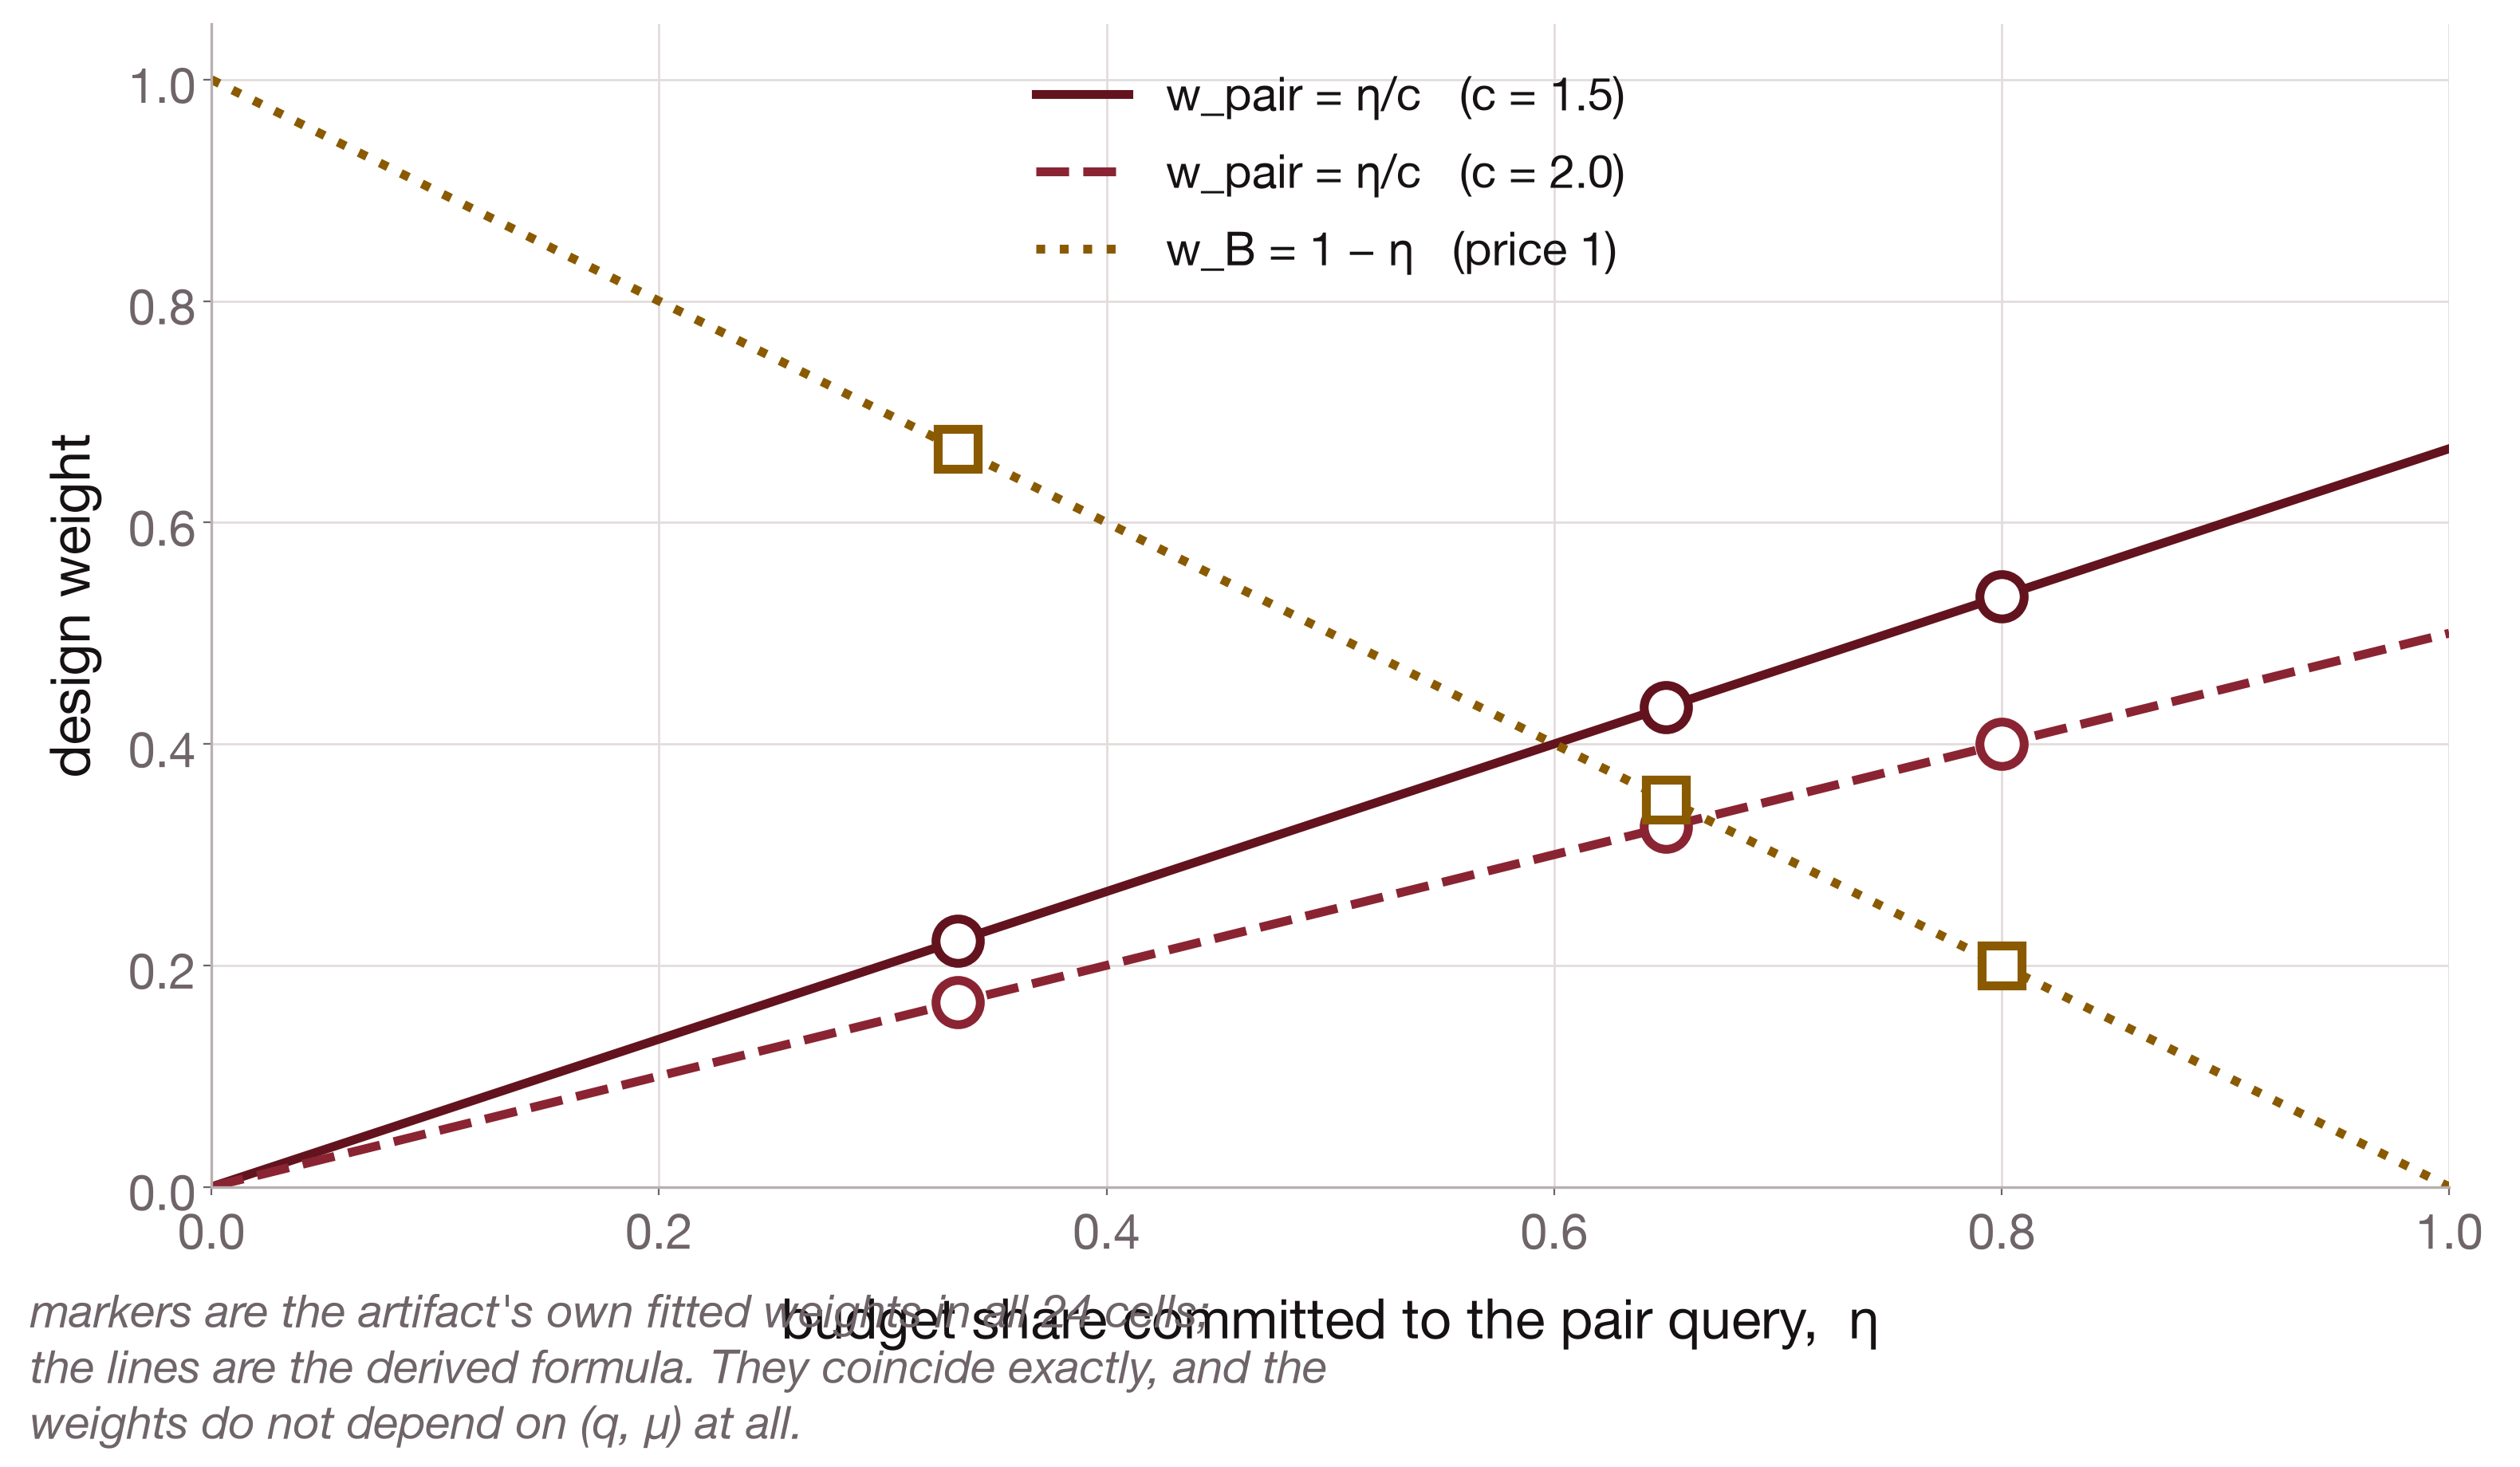
\includegraphics[width=\columnwidth]{d6_fig1_design.png}
\caption{Derived weights against the budget split. The lines are the formula
\eqref{eq:d6-design}; the markers are the artifact's own fitted weights in all $24$ cells. They
coincide exactly, and as Corollary~\ref{cor:d6-indep} predicts the weights do not depend on
$(q,\mu)$, so each marker stands for several cells differing in $(q,\mu)$.}
\label{fig:d6-design}
\end{figure}

\subsection{The Margin-Sensitive Exchange Law}
\label{sec:d6-margin}

The results so far concern the alternative family and the design. A sharper object is
available from the same development: an exchange bound in which the \emph{margin} between
selected and unselected coordinates appears explicitly.

\begin{lemma}[Score surplus from a common margin]
\label{lem:d6-surplus}
Let $A,B$ be finite with $|A|=|B|$ and suppose every element of $A$ beats every element of
$B$ by at least $\mu$ in $\mathrm{score}$. Then
\begin{equation}
|A|\,\mu\;\leq\;\sum_{i\in A}\mathrm{score}(i)-\sum_{j\in B}\mathrm{score}(j).
\label{eq:d6-surplus}
\end{equation}
\end{lemma}

\begin{proof}
If $B$ is empty both sides vanish. Otherwise take $b\in B$ maximising $\mathrm{score}$ on
$B$. Summing $\mu+\mathrm{score}(b)\le\mathrm{score}(i)$ over $A$ gives
$|A|(\mu+\mathrm{score}(b))\le\sum_{A}\mathrm{score}$, and
$\sum_{B}\mathrm{score}\le|B|\mathrm{score}(b)=|A|\mathrm{score}(b)$; subtracting gives
\eqref{eq:d6-surplus}.
\end{proof}

\leanbox{\lean{score\_surplus\_ge\_card\_mul\_margin} in
\lean{LeanD6MarginSensitiveExchangeV1}}

The lemma is pure finite combinatorics---no geometry, no design---and it is stated separately
because it is what converts a margin hypothesis into a quantity the exchange bound can
consume.

\begin{theorem}[Exchange bound retaining the surplus]
\label{thm:d6-exchange}
With $T$ Top-$k$ by $\mathrm{osc}\circ Q$ and $|S|=k$, writing $A=T\setminus S$ and
$B=S\setminus T$,
\begin{equation}
L_{F}(T)-L_{F}(S)\;\leq\;|A|\,\delta
 \;-\;\frac{1}{2}\Bigl(\sum_{j\in A}\mathrm{osc}(Q_{j})-\sum_{j\in B}\mathrm{osc}(Q_{j})\Bigr).
\label{eq:d6-exchangesurplus}
\end{equation}
\end{theorem}

\leanbox{\lean{pair\_loss\_le\_sdiff\_card\_sub\_score\_surplus} in
\lean{LeanD6MarginSensitiveExchangeV1}}

The bracketed term is the surplus. An earlier endpoint-patch argument dropped it and retained
only $|A|\delta$; because $T$ is Top-$k$ the surplus is non-negative, so
\eqref{eq:d6-exchangesurplus} is never weaker and is strictly stronger whenever the selected
scores exceed the unselected ones.

\begin{theorem}[Margin-sensitive exchange]
\label{thm:d6-marginexchange}
If in addition every selected coordinate beats every unselected one by at least $\mu$, then
\begin{equation}
2\bigl(L_{F}(T)-L_{F}(S)\bigr)\;\leq\;|T\setminus S|\;\bigl(2\delta-\mu\bigr).
\label{eq:d6-marginexchange}
\end{equation}
\end{theorem}

\begin{proof}
Apply Theorem~\ref{thm:d6-exchange}, then bound the surplus below by Lemma~\ref{lem:d6-surplus}
with $\mathrm{score}=\mathrm{osc}\circ Q$, using $|T\setminus S|=|S\setminus T|$ which holds
because $|T|=|S|$.
\end{proof}

\leanbox{\lean{pair\_doubled\_loss\_le\_card\_mul\_two\_delta\_sub\_margin} in
\lean{LeanD6MarginSensitiveExchangeV1}}

\noindent\emph{Supporting results in \lean{LeanD6MarginSensitiveExchangeV1}.}~These are the exchange law. The surplus lemma is pure finite combinatorics with no geometry in it, and it is what converts a margin hypothesis into a quantity the exchange bound can consume. The two exchange statements are ordered so that the first retains the surplus the earlier endpoint-patch argument discarded, and the second bounds that surplus below by the margin. They are reproduced as the prover has them; a further $0$ audited declarations in this module are positivity checks and measurability side conditions and are not displayed.

\noindent\textbf{S\,5}\quad\lean{pair\_doubled\_loss\_le\_card\_mul\_two\_delta\_sub\_margin}
{\footnotesize\[ \begin{aligned}[t]
&\{ \mathit{n} : \mathbb{N} \},\; (\mathit{q} : \mathit{Fin} (\mathit{n} + 1) \to \mathit{U} \to \mathbb{R} ),\; (\mathit{F} : (\mathit{Fin} (\mathit{n} + 1) \to \mathit{U})\\
&\quad \to \mathbb{R} ),\; (\mathit{delta} \mathit{mu} : \mathbb{R} ),\; (\mathit{hWeight} : \forall \mathit{c}, 0 \leq\\
&\quad \mathit{jointWeight} \mathit{q} \mathit{c}),\; (\mathit{hNorm} : \textstyle\sum \mathit{c}, \mathit{jointWeight} \mathit{q} \mathit{c} = 1),\\
&\quad \; (\mathit{hDeltaNonneg} : 0 \leq \mathit{delta}),\; (\mathit{hdelta} : \forall (\mathit{i} : \mathit{Fin} (\mathit{n} + 1)) (\mathit{x} \mathit{c} :\\
&\quad \mathit{Fin} (\mathit{n} + 1) \to \mathit{U}), |\mathit{mixedDifference} \mathit{F} \mathit{i} \mathit{x} \mathit{c}| \leq \mathit{delta}),\\
&\quad \; (\mathit{selected} \mathit{competitor} : \mathit{Finset} (\mathit{Fin} (\mathit{n} + 1))),\; (\mathit{k} : \mathbb{N} ),\\
&\quad \; (\mathit{hTop} : \mathit{IsTopKByScore} (\mathbf{fun} \mathit{j} \mapsto \mathit{osc} (\mathit{productResponse} \mathit{q} \mathit{F} \mathit{j}))\\
&\quad \mathit{selected} \mathit{k}),\; (\mathit{hCompetitorCard} : \mathit{competitor}.\mathit{card} = \mathit{k}),\\
&\quad \; (\mathit{hMargin} : \forall \mathit{i} \in \mathit{selected}, \forall \mathit{j} \notin \mathit{selected}, \mathit{mu} + \mathit{osc} (\\
&\quad \mathit{productResponse} \mathit{q} \mathit{F} \mathit{j}) \leq \mathit{osc} (\mathit{productResponse} \mathit{q} \mathit{F} \mathit{i}))\\
\vdash\;&2 * (\mathit{productCompressionLoss} \mathit{F} (\mathit{productResponse} \mathit{q} \mathit{F}) \mathit{selected}\\
&\quad - \mathit{productCompressionLoss} \mathit{F} (\mathit{productResponse} \mathit{q} \mathit{F}) \mathit{competitor})\\
&\quad \leq ((\mathit{selected} \ \mathit{competitor}).\mathit{card} : \mathbb{R} ) * (2 * \mathit{delta} - \mathit{mu})
\end{aligned} \]}

\noindent\textbf{S\,6}\quad\lean{pair\_loss\_le\_sdiff\_card\_sub\_score\_surplus}
{\footnotesize\[ \begin{aligned}[t]
&\{ \mathit{n} : \mathbb{N} \},\; (\mathit{q} : \mathit{Fin} (\mathit{n} + 1) \to \mathit{U} \to \mathbb{R} ),\; (\mathit{F} : (\mathit{Fin} (\mathit{n} + 1) \to \mathit{U})\\
&\quad \to \mathbb{R} ),\; (\mathit{delta} : \mathbb{R} ),\; (\mathit{hWeight} : \forall \mathit{c}, 0 \leq \mathit{jointWeight} \mathit{q} \mathit{c}),\\
&\quad \; (\mathit{hNorm} : \textstyle\sum \mathit{c}, \mathit{jointWeight} \mathit{q} \mathit{c} = 1),\; (\mathit{hDeltaNonneg} : 0 \leq\\
&\quad \mathit{delta}),\; (\mathit{hdelta} : \forall (\mathit{i} : \mathit{Fin} (\mathit{n} + 1)) (\mathit{x} \mathit{c} : \mathit{Fin} (\mathit{n} + 1) \to \mathit{U}),\\
&\quad |\mathit{mixedDifference} \mathit{F} \mathit{i} \mathit{x} \mathit{c}| \leq \mathit{delta}),\; (\mathit{selected} \mathit{competitor} :\\
&\quad \mathit{Finset} (\mathit{Fin} (\mathit{n} + 1))),\; (\mathit{k} : \mathbb{N} ),\; (\mathit{hTop} : \mathit{IsTopKByScore} (\mathbf{fun} \mathit{j}\\
&\quad \mapsto \mathit{osc} (\mathit{productResponse} \mathit{q} \mathit{F} \mathit{j})) \mathit{selected} \mathit{k}),\; (\mathit{hCompetitorCard}\\
&\quad : \mathit{competitor}.\mathit{card} = \mathit{k})\\
\vdash\;&\mathit{productCompressionLoss} \mathit{F} (\mathit{productResponse} \mathit{q} \mathit{F}) \mathit{selected} -\\
&\quad \mathit{productCompressionLoss} \mathit{F} (\mathit{productResponse} \mathit{q} \mathit{F}) \mathit{competitor} \leq\\
&\quad ((\mathit{selected} \ \mathit{competitor}).\mathit{card} : \mathbb{R} ) * \mathit{delta} - ((\mathit{selected}\\
&\quad \ \mathit{competitor}).\mathit{sum} (\mathbf{fun} \mathit{j} \mapsto \mathit{osc} (\mathit{productResponse} \mathit{q} \mathit{F} \mathit{j})) - (\\
&\quad \mathit{competitor} \ \mathit{selected}).\mathit{sum} (\mathbf{fun} \mathit{j} \mapsto \mathit{osc} (\mathit{productResponse} \mathit{q} \mathit{F} \mathit{j}))\\
&\quad ) / 2
\end{aligned} \]}

\noindent\textbf{S\,7}\quad\lean{score\_surplus\_ge\_card\_mul\_margin}
{\footnotesize\[ \begin{aligned}[t]
&\{ \mathit{I} : \mathit{Type}*\},\; [\mathit{DecidableEq} \mathit{I}],\; (\mathit{A} \mathit{B} : \mathit{Finset} \mathit{I}),\\
&\quad \; (\mathit{score} : \mathit{I} \to \mathbb{R} ),\; (\mathit{mu} : \mathbb{R} ),\; (\mathit{hCard} : \mathit{A}.\mathit{card} = \mathit{B}.\mathit{card}),\\
&\quad \; (\mathit{hMargin} : \forall \mathit{i} \in \mathit{A}, \forall \mathit{j} \in \mathit{B}, \mathit{mu} + \mathit{score} \mathit{j} \leq \mathit{score} \mathit{i})\\
\vdash\;&(\mathit{A}.\mathit{card} : \mathbb{R} ) * \mathit{mu} \leq \mathit{A}.\mathit{sum} \mathit{score} - \mathit{B}.\mathit{sum} \mathit{score}
\end{aligned} \]}


No symmetry is assumed, no active cell is fixed, and the reference is an arbitrary product
reference. The improvement over the $\delta$-only form is exactly $|T\setminus S|\mu$, which
is what makes the next subsection possible.

\subsection{The Sharp Threshold at Margin $2\delta$}
\label{sec:d6-threshold}

Equation \eqref{eq:d6-marginexchange} has an immediate consequence: at margin $2\delta$ the
right-hand side turns non-positive.

\begin{theorem}[Sufficiency]
\label{thm:d6-sufficient}
If $2\delta\leq\rho$ then $L_{F}(T)\leq L_{F}(S)$ for every $S$ with $|S|=k$.
\end{theorem}

\begin{proof}
By Theorem~\ref{thm:d6-marginexchange} the doubled difference is at most
$|T\setminus S|(2\delta-\rho)\le0$.
\end{proof}

\leanbox{\lean{margin\_two\_sufficient} in \lean{LeanD6SharpMarginThresholdV1}}

Theorem~\ref{thm:d6-sufficient} holds for \emph{every} product reference, including degenerate
ones, because its proof uses only the mixed-difference bound and the weight axioms. That
matters because the matching necessity result does not.

\begin{theorem}[The steering construction attains the bound exactly]
\label{thm:d6-steered}
For $A$ a coordinate set, $j\notin A$, $1\le\rho$, with $|A^{\complement}|=|A|$ and at least
two coordinates outside $A\cup\{j\}$, under the corner reference
\begin{equation}
2\bigl(L(A)-L(A^{\complement})\bigr)\;=\;|A|\,(2-\rho).
\label{eq:d6-steered}
\end{equation}
\end{theorem}

\leanbox{\lean{steered\_exchange\_equality} in \lean{LeanD6SharpMarginThresholdV1}}

\begin{theorem}[Every sub-threshold margin fails]
\label{thm:d6-subthreshold}
For $A$ non-empty and every $\rho\in[1,2)$, $A$ is Top-$k$ by the oscillation score and yet
$L(A^{\complement})<L(A)$.
\end{theorem}

\begin{proof}
$A$ is Top-$k$ by construction, and by \eqref{eq:d6-steered} the doubled difference equals
$|A|(2-\rho)>0$.
\end{proof}

\leanbox{\lean{every\_subthreshold\_margin\_fails} in
\lean{LeanD6SharpMarginThresholdV1}}

\noindent\emph{Supporting results in \lean{LeanD6SharpMarginThresholdV1}.}~These are the threshold. Sufficiency is proved for an arbitrary product reference, including degenerate ones, because its proof uses only the mixed-difference bound and the weight axioms. The equality statement and the sub-threshold failure are both under the corner reference, which is the asymmetry Section~\ref{sec:d6-discussion} reports and the reference sweep of Section~\ref{sec:d6-results} quantifies. They are reproduced as the prover has them; a further $0$ audited declarations in this module are positivity checks and measurability side conditions and are not displayed.

\noindent\textbf{S\,8}\quad\lean{every\_subthreshold\_margin\_fails}
{\footnotesize\[ \begin{aligned}[t]
&\{ \mathit{n} : \mathbb{N} \},\; (\mathit{A} : \mathit{Finset} (\mathit{I} \mathit{n})),\; (\mathit{j} : \mathit{I} \mathit{n}),\; (\mathit{hj} : \mathit{j} \notin \mathit{A}),\\
&\quad \; (\mathit{hne} : \mathit{A}.\mathit{Nonempty}),\; (\mathit{rho} : \mathbb{R} ),\; (\mathit{hr} : 1 \leq \mathit{rho}),\\
&\quad \; (\mathit{hr2} : \mathit{rho} < 2),\; (\mathit{hbal} : \mathit{Aᶜ}.\mathit{card}=\mathit{A}.\mathit{card}),\\
&\quad \; (\mathit{hB} : 2 \leq (\mathit{others} \mathit{A} \mathit{j}).\mathit{card})\\
\vdash\;&\mathit{IsTopKByScore} (\mathbf{fun} \mathit{i} => \mathit{osc} (\mathit{productResponse} \mathit{corner} (\mathit{steered}\\
&\quad \mathit{A} \mathit{j} \mathit{rho}) \mathit{i})) \mathit{A} \mathit{A}.\mathit{card} \wedge \mathit{productCompressionLoss} (\mathit{steered} \mathit{A} \mathit{j} \mathit{rho}) (\\
&\quad \mathit{productResponse} \mathit{corner} (\mathit{steered} \mathit{A} \mathit{j} \mathit{rho})) \mathit{Aᶜ} <\\
&\quad \mathit{productCompressionLoss} (\mathit{steered} \mathit{A} \mathit{j} \mathit{rho}) (\mathit{productResponse}\\
&\quad \mathit{corner} (\mathit{steered} \mathit{A} \mathit{j} \mathit{rho})) \mathit{A}
\end{aligned} \]}

\noindent\textbf{S\,9}\quad\lean{margin\_two\_sufficient}
{\footnotesize\[ \begin{aligned}[t]
&\{ \mathit{U} : \mathit{Type}*\},\; [\mathit{Fintype} \mathit{U}],\; [\mathit{Nonempty} \mathit{U}],\; \{ \mathit{n} : \mathbb{N} \},\; (\mathit{q} : \mathit{I} \mathit{n} \to\\
&\quad \mathit{U} \to \mathbb{R} ),\; (\mathit{F} : (\mathit{I} \mathit{n} \to \mathit{U}) \to \mathbb{R} ),\; (\mathit{delta} \mathit{rho} : \mathbb{R} ),\\
&\quad \; (\mathit{hWeight} : \forall \mathit{c},0 \leq \mathit{jointWeight} \mathit{q} \mathit{c}),\; (\mathit{hNorm} : \textstyle\sum \mathit{c},\\
&\quad \mathit{jointWeight} \mathit{q} \mathit{c}=1),\; (\mathit{hd} : 0 \leq \mathit{delta}),\; (\mathit{hdelta} : \forall \mathit{i} \mathit{x} \mathit{c},\\
&\quad |\mathit{mixedDifference} \mathit{F} \mathit{i} \mathit{x} \mathit{c}| \leq \mathit{delta}),\; (\mathit{T} : \mathit{Finset} (\mathit{I} \mathit{n})),\\
&\quad \; (\mathit{k} : \mathbb{N} ),\; (\mathit{htop} : \mathit{IsTopKByScore} (\mathbf{fun} \mathit{i} => \mathit{osc} (\\
&\quad \mathit{productResponse} \mathit{q} \mathit{F} \mathit{i})) \mathit{T} \mathit{k}),\; (\mathit{hmargin} : \forall \mathit{i} \in \mathit{T},\forall \mathit{j} \notin \mathit{T},\\
&\quad \mathit{rho}+\mathit{osc} (\mathit{productResponse} \mathit{q} \mathit{F} \mathit{j}) \leq \mathit{osc} (\mathit{productResponse} \mathit{q} \mathit{F} \mathit{i})\\
&\quad ),\; (\mathit{hrho} : 2*\mathit{delta} \leq \mathit{rho}),\; (\mathit{S} : \mathit{Finset} (\mathit{I} \mathit{n})),\\
&\quad \; (\mathit{hS} : \mathit{S}.\mathit{card}=\mathit{k})\\
\vdash\;&\mathit{productCompressionLoss} \mathit{F} (\mathit{productResponse} \mathit{q} \mathit{F}) \mathit{T} \leq\\
&\quad \mathit{productCompressionLoss} \mathit{F} (\mathit{productResponse} \mathit{q} \mathit{F}) \mathit{S}
\end{aligned} \]}

\noindent\textbf{S\,10}\quad\lean{steered\_exchange\_equality}
{\footnotesize\[ \begin{aligned}[t]
&\{ \mathit{n} : \mathbb{N} \},\; (\mathit{A} : \mathit{Finset} (\mathit{I} \mathit{n})),\; (\mathit{j} : \mathit{I} \mathit{n}),\; (\mathit{hj} : \mathit{j} \notin \mathit{A}),\; (\mathit{rho} : \mathbb{R} ),\\
&\quad \; (\mathit{hr} : 1 \leq \mathit{rho}),\; (\mathit{hbal} : \mathit{Aᶜ}.\mathit{card}=\mathit{A}.\mathit{card}),\\
&\quad \; (\mathit{hB} : 2 \leq (\mathit{others} \mathit{A} \mathit{j}).\mathit{card})\\
\vdash\;&2*(\mathit{productCompressionLoss} (\mathit{steered} \mathit{A} \mathit{j} \mathit{rho}) (\mathit{productResponse}\\
&\quad \mathit{corner} (\mathit{steered} \mathit{A} \mathit{j} \mathit{rho})) \mathit{A}- \mathit{productCompressionLoss} (\mathit{steered} \mathit{A} \mathit{j}\\
&\quad \mathit{rho}) (\mathit{productResponse} \mathit{corner} (\mathit{steered} \mathit{A} \mathit{j} \mathit{rho})) \mathit{Aᶜ})=\\
&\quad (\mathit{A}.\mathit{card}:\mathbb{R} )*(2-\mathit{rho})
\end{aligned} \]}


Together these make the condition $\rho\ge2\delta$ sharp at $\delta=1$: sufficient for
Top-$C$ optimality, and violated for every $\rho$ in $[1,2)$.

Three scope statements belong here rather than in the Discussion, because the result invites
over-reading. It is a Top-$C$ optimality threshold, not a minimax value: it says when the
Top-$C$ rule is optimal among same-cardinality sets, and says nothing about the minimax value
of the whole same-response fibre, which is a different quantifier and is open. Sufficiency and
necessity do not share a reference class, as noted above. And robustness to the reference
was measured rather than assumed: an exact rational sweep of the product reference
$q_{i}(1)=t$, reported in Section~\ref{sec:d6-results}, finds that the witness does not collapse
the moment the corner is left but degrades continuously, and fails only past a breakdown point
$t^{\star}(\mu)$ that grows with the margin and is never reached at $\mu=2$. The mechanism is
that the steered coordinate $j$ accumulates span as the reference acquires interior mass, so
the separation the corner enforces between $A$ and its complement narrows until $j$ overtakes
$A$ on score and $A$ is no longer the Top-$C$ set.

\begin{figure}[htbp]
\centering
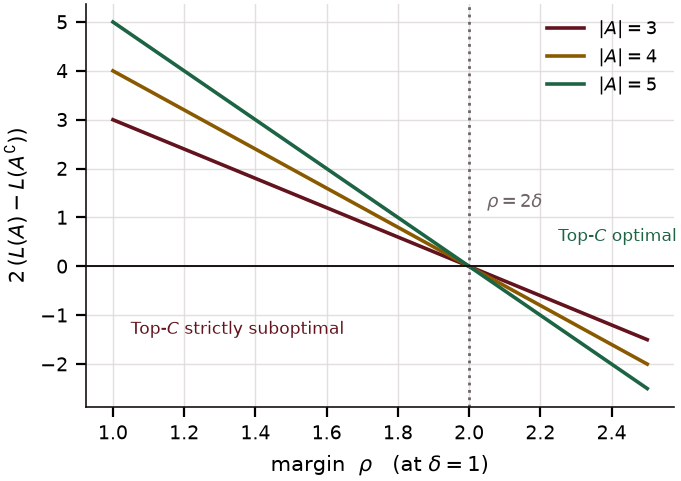
\includegraphics[width=\columnwidth]{d6_fig3_threshold.png}
\caption{The exchange law of \lean{steered\_exchange\_equality}, drawn at $\delta=1$. The
doubled regret of the Top-$C$ set against its complement is exactly $|A|(2-\rho)$: positive
below the threshold $\rho=2\delta$, where the construction of
Theorem~\ref{thm:d6-subthreshold} makes Top-$C$ strictly worse than a same-cardinality
competitor, and non-positive at and above it, where Theorem~\ref{thm:d6-sufficient} forbids any
competitor from beating it. The two theorems meet at $\rho=2$ with no gap between them, which
is what makes the threshold sharp rather than merely bracketed. The lines are the proved
identity evaluated, not a fit, and the slope $-|A|$ is why a larger selected set is penalised
more by the same margin deficit.}
\label{fig:d6-threshold}
\end{figure}

\subsection{The Separation Certificate on a Cell}
\label{sec:d6-certificate}

A separate question is whether a claimed strict separation survives across a whole parameter
cell rather than at sampled points.

\begin{lemma}[Quadratic infimum on an interval]
\label{lem:d6-quadinf}
For $f(x)=ax^{2}+bx+c$ with $a\ge0$ on $[l,u]$,
$\inf_{[l,u]}f=\min\{f(l),f(u),f(x^{\dagger})\}$ with $x^{\dagger}=-b/2a$ when $a>0$ and
$x^{\dagger}\in[l,u]$.
\end{lemma}

\leanbox{\lean{quadratic\_inf\_Icc} in \lean{LeanD6AlternativeReductionV1}}

\begin{theorem}[Separation across a cell]
\label{thm:d6-modulus}
On a cell $[t_{0},t_{1}]$, if
\begin{equation}
L_{\mathrm{full}}(t_{0})\;>\;\rho_{\mathrm{two}}\;U_{\mathrm{two}}(t_{0}),
\qquad \rho\;=\;r^{(t_{1}-t_{0})/q},
\label{eq:d6-modulus}
\end{equation}
then the strict separation holds throughout the cell.
\end{theorem}

\leanbox{\lean{no\_crossing\_of\_modulus}, \lean{crossing\_bracket} in
\lean{LeanD6AlternativeReductionV1}}

\noindent\emph{Supporting results in \lean{LeanD6AlternativeReductionV1}.}~These are the certificate machinery. The quadratic infimum is given at the vertex and at each endpoint separately, which is what reduces a continuous range of $x$ to three evaluations; the crossing statements then propagate the verdict across a cell by an exact multiplicative factor rather than by sampling within it. They are reproduced as the prover has them; a further $4$ audited declarations in this module are positivity checks and measurability side conditions and are not displayed.

\noindent\textbf{S\,11}\quad\lean{crossing\_bracket}
{\footnotesize\[ \begin{aligned}[t]
&(\mathit{f} : \mathbb{R} \to \mathbb{R} ),\; (\mathit{t0} \mathit{t1} : \mathbb{R} ),\; (\mathit{ht} : \mathit{t0} \leq \mathit{t1}),\; (\mathit{hc} :\\
&\quad \mathit{ContinuousOn} \mathit{f} (\mathit{Set}.\mathit{Icc} \mathit{t0} \mathit{t1})),\; (\mathit{h0} : \mathit{f} \mathit{t0} \leq 0),\; (\mathit{h1} : 0 \leq \mathit{f} \mathit{t1})\\
\vdash\;&\exists \mathit{t} \in \mathit{Set}.\mathit{Icc} \mathit{t0} \mathit{t1}, \mathit{f} \mathit{t} = 0
\end{aligned} \]}

\noindent\textbf{S\,12}\quad\lean{no\_crossing\_of\_modulus}
{\footnotesize\[ \begin{aligned}[t]
&(\mathit{f} : \mathbb{R} \to \mathbb{R} ),\; (\mathit{t0} \mathit{t1} \mathit{Lip} \mathit{m} : \mathbb{R} ),\; (\mathit{ht} : \mathit{t0} \leq \mathit{t1}),\\
&\quad \; (\mathit{hLip} : 0 \leq \mathit{Lip}),\; (\mathit{hlip} : \forall \mathit{s} \in \mathit{Set}.\mathit{Icc} \mathit{t0} \mathit{t1}, |\mathit{f} \mathit{s} - \mathit{f} \mathit{t0}| \leq\\
&\quad \mathit{Lip} * (\mathit{s} - \mathit{t0})),\; (\mathit{hm} : \mathit{m} \leq \mathit{f} \mathit{t0}),\; (\mathit{hpos} : 0 < \mathit{m}),\\
&\quad \; (\mathit{hgap} : \mathit{Lip} * (\mathit{t1} - \mathit{t0}) < \mathit{m})\\
\vdash\;&\forall \mathit{t} \in \mathit{Set}.\mathit{Icc} \mathit{t0} \mathit{t1}, 0 < \mathit{f} \mathit{t}
\end{aligned} \]}

\noindent\textbf{S\,13}\quad\lean{quadratic\_inf\_attained}
{\footnotesize\[ \begin{aligned}[t]
&(\mathit{a} \mathit{b} \mathit{c} \mathit{lo} \mathit{hi} : \mathbb{R} ),\; (\mathit{ha} : 0 < \mathit{a}),\; (\mathit{hv1} : \mathit{lo} \leq -\mathit{b} / (2 * \mathit{a})),\\
&\quad \; (\mathit{hv2} : -\mathit{b} / (2 * \mathit{a}) \leq \mathit{hi})\\
\vdash\;&(\forall \mathit{x}, \mathit{lo} \leq \mathit{x} \to \mathit{x} \leq \mathit{hi} \to \mathit{a} * (-\mathit{b} / (2 * \mathit{a})) ^{2} + \mathit{b} * (-\mathit{b} / (\\
&\quad 2 * \mathit{a})) + \mathit{c} \leq \mathit{a} * \mathit{x} ^{2} + \mathit{b} * \mathit{x} + \mathit{c}) \wedge \mathit{lo} \leq -\mathit{b} / (2 * \mathit{a}) \wedge\\
&\quad -\mathit{b} / (2 * \mathit{a}) \leq \mathit{hi}
\end{aligned} \]}


The information \eqref{eq:d6-ib} is quadratic in $x$ with non-negative leading coefficient, so
Lemma~\ref{lem:d6-quadinf} reduces a continuous $x$-range to three evaluations. Both verdicts use
outward \emph{rational} enclosures and exact gaps rather than floating point, so a certificate
is a proof about the cell and not a statement about the points sampled in it.

\begin{figure}[htbp]
\centering
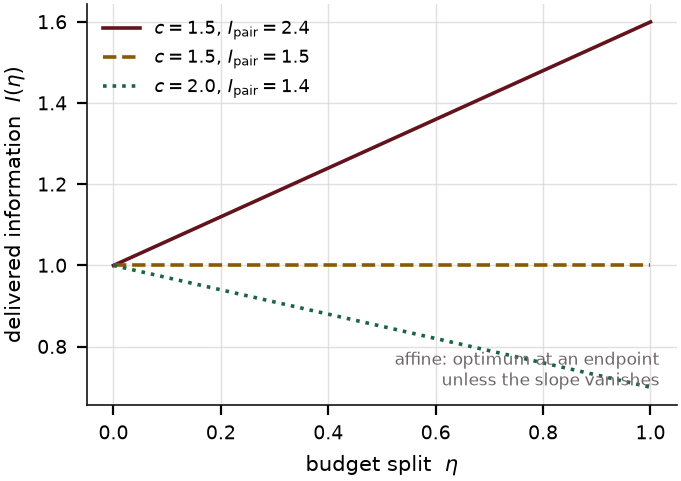
\includegraphics[width=\columnwidth]{d6_fig4_affine.png}
\caption{Why the optimal design is pure except on a threshold. Theorem~\ref{thm:d6-affine} makes
delivered information affine in the budget split $\eta$, so $I(\eta)$ is a straight line
between $I_{B}$ at $\eta=0$ and $I_{\mathrm{pair}}/c$ at $\eta=1$, whatever the parameters.
An affine function on an interval attains its maximum at an endpoint unless its slope is
zero, so the optimum is pure---all budget to one query type---except on the single surface
$I_{\mathrm{pair}}=c\,I_{B}$ where the line is flat and every split is optimal. The three
lines show the two strict cases and the degenerate one. Exact evaluation of
\eqref{eq:d6-transitioncond}.}
\label{fig:d6-affine}
\end{figure}


\section{Part II: The Geometry of the Alternative, and What a Scalar Proxy Loses}

\label{sec:fn-setting}

\subsection{Framework Overview}

The design buys precision $\alpha_{ra}$ at each cell $(r,a)$, and the energy of an
alternative $\lambda$ is the quadratic form
$\tfrac12(\lambda-\mu)^{\top}M(x)(\lambda-\mu)$. An alternative is \emph{relevant} if it
would change the Top-$k$ answer, that is, if some $j\notin T$ overtakes some $i\in T$ in
capacity.

A distinction is maintained throughout. $J_{\mathrm{full}}$ is a normative quantity---the
infimum of the energy over the relevant alternative set. The development below proves each
component of a computation for it and proves the inequalities \eqref{eq:fn-order} between the
three quantities, but it does not define $J_{\mathrm{full}}$ as a formalised infimum, and it
does not claim the components assemble into an equality. That distinction is carried into
Section~\ref{sec:fn-discussion} rather than elided.

\subsection{What the Scalar Proxy Is, Exactly}
\label{sec:fn-proxydef}

Since the paper's first claim is that a particular approximation fails, the approximation
must be pinned down. Given the truth $\mu$, a claimed top relation $i$ and a challenger $j$,
let $a^{\circ},b^{\circ}$ be the cells attaining $i$'s current max and min, and
$c^{\circ},d^{\circ}$ those attaining $j$'s. The scalar proxy is the value of the inner
problem at those four cells with the ordering constraints dropped:
\begin{equation}
J_{\mathrm{scalar}}
\;=\;
\frac{\bigl(C_{i}(\mu)-C_{j}(\mu)\bigr)^{2}}
     {2\Bigl(\frac{1}{\alpha_{ia^{\circ}}}+\frac{1}{\alpha_{ib^{\circ}}}
            +\frac{1}{\alpha_{jc^{\circ}}}+\frac{1}{\alpha_{jd^{\circ}}}\Bigr)} .
\label{eq:fn-scalar}
\end{equation}

Two approximations are folded into \eqref{eq:fn-scalar} and they fail independently. The first
is that the extrema stay where they are: the four cells are read off $\mu$ and never
revisited, so an alternative that changes which cell is extremal is invisible. The second is
that the ordering constraints defining a pair region are dropped, so an alternative that
would have to satisfy them is charged too little. Family~1 below exploits the first, family~2
the second.

Equation \eqref{eq:fn-scalar} is not a strawman. It is the natural transport of the
fixed-confidence inner problem to this setting, it is cheap---four lookups and an arithmetic
expression---and it agrees with $J_{\mathrm{full}}$ whenever the extrema happen not to move.
The question is whether that agreement can be relied on.

\subsection{Simplifying Assumptions}

\begin{enumerate}
\item[1)] \textbf{Free response table.} Every cell $(r,a)$ may take any real value; no
parametric form links cells within a relation. This is what makes the alternative set a
polyhedral union rather than a curved manifold.

\item[2)] \textbf{Known variance, positive precision.} Precisions $\alpha_{ra}$ are known and
strictly positive wherever they appear in a denominator. Under realizability coupling---where
the precision at one cell constrains another---the cost does not separate, and nothing here
covers that case.

\item[3)] \textbf{Quadratic energy.} The energy is $\tfrac12(\lambda-\mu)^{\top}M(\lambda-\mu)$
with $M$ symmetric positive semidefinite. Semidefiniteness rather than definiteness is
assumed deliberately, for the reason given in the Background.

\item[4)] \textbf{Finite action set.} Each relation has finitely many actions, so the union in
\eqref{eq:fn-J} is over a finite index set and step 1 of the procedure terminates.
\end{enumerate}

\subsection{Why a Range Target Is Not a Mean Target}

The difficulty is specific to ranking by a range, and isolating it explains why the rest of
the development takes the form it does.

When relations are ranked by a mean, the comparison $\mu_{j}\ge\mu_{i}$ is a single linear
inequality, so the relevant alternative set is a half-space---convex, with one facet, and
with a closed-form nearest point under any quadratic energy. There is nothing further to
decide.

When relations are ranked by a range, the comparison hides four extremal choices, and which
cells attain them depends on $\lambda$. The set $\{\lambda:C_{j}(\lambda)\ge C_{i}(\lambda)\}$
is not convex: it is a union of polyhedra, one per choice of attaining pair, and the
minimiser may sit in a piece whose attaining cells differ from the truth's. Any procedure
that fixes the attaining cells in advance is therefore solving a \emph{restriction} of the
problem, and a restriction can have a strictly larger value. That last sentence is the entire
mechanism behind family~1.

\subsection{The Finite Max/Min Set Identity}
\label{sec:fn-union}

\begin{theorem}[Union identity]
\label{thm:fn-union}
For relations $i,j$ and any alternative $\lambda$,
\begin{multline}
C_{j}(\lambda)\geq C_{i}(\lambda)
\;\;\Longleftrightarrow\;\;
\exists\,a,b\;\;\forall\,u,v:\\
\lambda_{ja}-\lambda_{jb}\;\geq\;\lambda_{iu}-\lambda_{iv}.
\label{eq:fn-union}
\end{multline}
\end{theorem}

\begin{proof}
($\Rightarrow$) Choose $a$ attaining $\max_{a}\lambda_{ja}$ and $b$ attaining
$\min_{b}\lambda_{jb}$, so $\lambda_{ja}-\lambda_{jb}=C_{j}(\lambda)$. For any $u,v$,
$\lambda_{iu}-\lambda_{iv}\le C_{i}(\lambda)\le C_{j}(\lambda)$.

($\Leftarrow$) Given such $a,b$, the range of $j$ is at least $\lambda_{ja}-\lambda_{jb}$,
which dominates every pair difference in $i$; taking the maximum over $i$'s pairs gives
$C_{j}(\lambda)\ge C_{i}(\lambda)$.
\end{proof}

\leanbox{\lean{range\_ge\_iff\_exists\_pair} in
\lean{LeanFunctionalRangeAlternativeUnionV1}}

This is the model bridge and the step that makes everything else possible. It converts a
statement about extrema---objects that move with $\lambda$---into a statement about a
\emph{fixed} pair $(a,b)$, at the cost of an existential over finitely many pairs. The
quantifier in \eqref{eq:fn-union} ranges over the \emph{alternative's} extrema, never the
truth's; freezing them there is exactly the error the families quantify.

\begin{definition}[Pair region]
\begin{equation}
\mathcal{P}_{ijab}=\bigl\{\lambda:\;
\lambda_{iu}-\lambda_{iv}-\lambda_{ja}+\lambda_{jb}\leq 0
\;\;\forall u,v\bigr\}.
\label{eq:fn-polyhedron}
\end{equation}
\end{definition}

\begin{proposition}[Convexity, unconditionally]
\label{prop:fn-convex}
Each $\mathcal{P}_{ijab}$ is convex, with no assumption on $M$.
\end{proposition}

\begin{proof}
Each constraint in \eqref{eq:fn-polyhedron} is linear in $\lambda$, so the region is an
intersection of half-spaces.
\end{proof}

\leanbox{\lean{alternative\_union\_polyhedra}, \lean{pairRegion\_convex} in
\lean{LeanFunctionalRangeAlternativeUnionV1}}

\noindent\emph{Supporting results in \lean{LeanFunctionalRangeAlternativeUnionV1}.}~These establish the geometry. The pair characterisation is the model bridge: it replaces the moving extrema by a fixed ordered pair at the cost of an existential over finitely many pairs. Convexity is proved with no assumption on the information matrix, which matters because the certificate later admits singular matrices, and the energy rewrites are what let the infimum be taken region by region. They are reproduced as the prover has them; a further $0$ audited declarations in this module are positivity checks and measurability side conditions and are not displayed.

\noindent\textbf{S\,1}\quad\lean{alternative\_union\_polyhedra}
{\footnotesize\[ \begin{aligned}[t]
&(\mathit{T} : \mathit{Finset} \mathit{R}),\; (\mathit{Q} : \mathit{R} \to \mathit{A} \to \mathbb{R} )\\
\vdash\;&\mathit{ClosedAlternative} \mathit{T} \mathit{Q} \leftrightarrow \exists \mathit{i} \in \mathit{T}, \exists \mathit{j}, \mathit{j} \notin \mathit{T} \wedge \exists \mathit{a} \mathit{b} : \mathit{A},\\
&\quad \mathit{PairRegion} \mathit{Q} \mathit{i} \mathit{j} \mathit{a} \mathit{b}
\end{aligned} \]}

\noindent\textbf{S\,2}\quad\lean{energy\_inf\_rewrite}
{\footnotesize\[ \begin{aligned}[t]
&(\mathit{T} : \mathit{Finset} \mathit{R}),\; (\mathit{E} : (\mathit{R} \to \mathit{A} \to \mathbb{R} ) \to \mathbb{R} )\\
\vdash\;&\mathit{sInf} \{ \mathit{z} : \mathbb{R} | \exists \mathit{Q}, \mathit{ClosedAlternative} \mathit{T} \mathit{Q} \wedge \mathit{E} \mathit{Q} = \mathit{z}\} = \mathit{sInf} \{ \mathit{z} : \mathbb{R} | \exists \mathit{i}\\
&\quad \in \mathit{T}, \exists \mathit{j}, \mathit{j} \notin \mathit{T} \wedge \exists \mathit{a} \mathit{b} : \mathit{A}, \exists \mathit{Q}, \mathit{PairRegion} \mathit{Q} \mathit{i} \mathit{j} \mathit{a} \mathit{b} \wedge \mathit{E} \mathit{Q} = \mathit{z}\}
\end{aligned} \]}

\noindent\textbf{S\,3}\quad\lean{energy\_sets\_equal}
{\footnotesize\[ \begin{aligned}[t]
&(\mathit{T} : \mathit{Finset} \mathit{R}),\; (\mathit{E} : (\mathit{R} \to \mathit{A} \to \mathbb{R} ) \to \mathbb{R} )\\
\vdash\;&\{ \mathit{z} : \mathbb{R} | \exists \mathit{Q}, \mathit{ClosedAlternative} \mathit{T} \mathit{Q} \wedge \mathit{E} \mathit{Q} = \mathit{z}\} = \{ \mathit{z} : \mathbb{R} | \exists \mathit{i} \in \mathit{T}, \exists \mathit{j},\\
&\quad \mathit{j} \notin \mathit{T} \wedge \exists \mathit{a} \mathit{b} : \mathit{A}, \exists \mathit{Q}, \mathit{PairRegion} \mathit{Q} \mathit{i} \mathit{j} \mathit{a} \mathit{b} \wedge \mathit{E} \mathit{Q} = \mathit{z}\}
\end{aligned} \]}

\noindent\textbf{S\,4}\quad\lean{not\_strictTopK\_iff}
{\footnotesize\[ \begin{aligned}[t]
&(\mathit{T} : \mathit{Finset} \mathit{R}),\; (\mathit{k} : \mathbb{N} ),\; (\mathit{hcard} : \mathit{T}.\mathit{card} = \mathit{k}),\\
&\quad \; (\mathit{Q} : \mathit{R} \to \mathit{A} \to \mathbb{R} )\\
\vdash\;&\neg \mathit{StrictTopK} (\mathbf{fun} \mathit{r} => \mathit{capacity} (\mathit{Q} \mathit{r})) \mathit{T} \mathit{k} \leftrightarrow \mathit{ClosedAlternative}\\
&\quad \mathit{T} \mathit{Q}
\end{aligned} \]}

\noindent\textbf{S\,5}\quad\lean{pairRegion\_convex}
{\footnotesize\[ (\mathit{i} \mathit{j} : \mathit{R}),\; (\mathit{a} \mathit{b} : \mathit{A}) \;\vdash\; \mathit{Convex} \mathbb{R} \{ \mathit{Q} : \mathit{R} \to \mathit{A} \to \mathbb{R} | \mathit{PairRegion} \mathit{Q} \mathit{i} \mathit{j} \mathit{a} \mathit{b}\} \]}

\noindent\textbf{S\,6}\quad\lean{pair\_le\_capacity}
{\footnotesize\[ (\mathit{f} : \mathit{A} \to \mathbb{R} ),\; (\mathit{a} \mathit{b} : \mathit{A}) \;\vdash\; \mathit{f} \mathit{a} - \mathit{f} \mathit{b} \leq \mathit{capacity} \mathit{f} \]}

\noindent\textbf{S\,7}\quad\lean{range\_ge\_iff\_exists\_pair}
{\footnotesize\[ \begin{aligned}[t]
&(\mathit{f} \mathit{g} : \mathit{A} \to \mathbb{R} )\\
\vdash\;&\mathit{capacity} \mathit{f} \leq \mathit{capacity} \mathit{g} \leftrightarrow \exists \mathit{a} \mathit{b} : \mathit{A}, \forall \mathit{u} \mathit{v} : \mathit{A}, \mathit{f} \mathit{u} - \mathit{f} \mathit{v} \leq \mathit{g} \mathit{a} - \mathit{g} \mathit{b}
\end{aligned} \]}


By Theorem~\ref{thm:fn-union} the relevant alternative set is the finite union
$\bigcup_{i,j,a,b}\mathcal{P}_{ijab}$, so the oracle is
\begin{equation}
J_\mu(x)\;=\;\min_{i\in T,\,j\notin T,\,a,b}\;
\inf_{\lambda\in\mathcal{P}_{ijab}}\;
\tfrac{1}{2}(\lambda-\mu)^{\top}M(x)(\lambda-\mu).
\label{eq:fn-J}
\end{equation}

\subsection{The Oracle Is a Finite Check}
\label{sec:fn-oracle}

\begin{theorem}[Finite check]
\label{thm:fn-oracle}
A number $c$ lower-bounds the energy over the whole alternative set if and only if it
lower-bounds it on every pair region.
\end{theorem}

\begin{proof}
($\Leftarrow$) Any $\lambda$ in the union lies in some region by Theorem~\ref{thm:fn-union}.
($\Rightarrow$) Each region is a subset of the union.
\end{proof}

\leanbox{\lean{energy\_lower\_bound\_iff}, \lean{energy\_ge\_of\_pairwise} in
\lean{LeanFunctionalRangeEnergyOracleV1}}

The index set in \eqref{eq:fn-J} is finite, so certifying reduces to a finite conjunction of
convex problems and no infimum over an infinite-dimensional set is ever taken. One
bookkeeping rule is maintained throughout and is worth stating because it is easy to violate:
a lower bound valid for \emph{every} region, and then their minimum, lower-bounds $J$; a
single feasible alternative only \emph{upper}-bounds it. Nothing in the development derives a
lower bound from an exhibited point.

\subsection{Shrink and Expand as Equivalences}
\label{sec:fn-shrink}

Certifying against a pair region reduces to two one-sided problems: shrinking the incumbent
$i$'s range below a level $z$ and expanding the challenger $j$'s above it. Both are stated as
equivalences rather than bounds, so that composing them relaxes nothing.

\begin{theorem}[Shrink]
\label{thm:fn-shrink}
$\mathrm{range}(\theta_{i})\le z$ if and only if all cells of $i$ lie in a common interval of
length $z$, and the cheapest such placement is coordinate-wise the clamp:
\begin{equation}
S_{i}(z)=\min_{\ell}\,\frac{1}{2}\sum_{a}\alpha_{ia}\;
\mathrm{dist}\bigl(\theta_{ia},\,[\ell,\ell+z]\bigr)^{2}.
\label{eq:fn-shrink}
\end{equation}
\end{theorem}

\begin{proof}
The equivalence is immediate from the definition of range. For the cost, fix $\ell$; for each
cell independently the closest point of $[\ell,\ell+z]$ is the clamp, proved by cases on
whether $\theta_{ia}$ lies below, inside or above the interval. The per-cell costs then sum
because the objective is separable given $\ell$.
\end{proof}

\leanbox{\lean{range\_le\_iff\_exists\_interval}, \lean{clamp\_dist\_le},
\lean{shrink\_lower} in \lean{LeanFunctionalShrinkExpandV1}}

\begin{theorem}[Expand]
\label{thm:fn-expand}
$\mathrm{range}(\theta_{j})\ge z$ if and only if some \emph{ordered} pair is separated by at
least $z$, and
\begin{equation}
E_{j}(z)=\min_{a\neq b}\;
\frac{\bigl[\,z-(\theta_{ja}-\theta_{jb})\,\bigr]_{+}^{2}}
     {2\bigl(\frac{1}{\alpha_{ja}}+\frac{1}{\alpha_{jb}}\bigr)}.
\label{eq:fn-expand}
\end{equation}
\end{theorem}

\begin{proof}
Again the equivalence is immediate. For the cost, the problem minimises a separable quadratic
subject to \emph{one} linear constraint $\lambda_{ja}-\lambda_{jb}\ge z$; the minimiser is
exhibited explicitly and the value computed by substitution, so \eqref{eq:fn-expand} is exact
rather than bounded.
\end{proof}

\leanbox{\lean{range\_ge\_iff\_exists\_pair\_ge}, \lean{expand\_lower} in
\lean{LeanFunctionalShrinkExpandV1}}

\noindent\emph{Supporting results in \lean{LeanFunctionalShrinkExpandV1}.}~These are the two one-sided problems. Each is stated as an equivalence and then given a cost, and each cost is proved both as a lower bound and as attained, so composing them relaxes nothing. The clamp lemmas carry the coordinate-wise argument that makes the shrink cost separable once the interval is fixed. They are reproduced as the prover has them; a further $7$ audited declarations in this module are positivity checks and measurability side conditions and are not displayed.

\noindent\textbf{S\,12}\quad\lean{range\_ge\_iff\_exists\_pair\_ge}
{\footnotesize\[ \begin{aligned}[t]
&(\mathit{lam} : \mathit{A} \to \mathbb{R} ),\; (\mathit{z} : \mathbb{R} )\\
\vdash\;&\mathit{z} \leq \mathit{rng} \mathit{lam} \leftrightarrow \exists \mathit{a} \mathit{b} : \mathit{A}, \mathit{z} \leq \mathit{lam} \mathit{a} - \mathit{lam} \mathit{b}
\end{aligned} \]}

\noindent\textbf{S\,13}\quad\lean{range\_le\_iff\_exists\_interval}
{\footnotesize\[ \begin{aligned}[t]
&(\mathit{lam} : \mathit{A} \to \mathbb{R} ),\; (\mathit{z} : \mathbb{R} )\\
\vdash\;&\mathit{rng} \mathit{lam} \leq \mathit{z} \leftrightarrow \exists \mathit{l} : \mathbb{R} , \forall \mathit{a} : \mathit{A}, \mathit{l} \leq \mathit{lam} \mathit{a} \wedge \mathit{lam} \mathit{a} \leq \mathit{l} + \mathit{z}
\end{aligned} \]}


The word \emph{ordered} in Theorem~\ref{thm:fn-expand} is load-bearing and was not in an earlier
version. Requiring an ordered pair means only two cells move; an unordered formulation forces
a third cell to accommodate the separation and overstates the cost, which would make the
oracle report alternatives as more expensive than they are.

\subsection{The Inner Problem in Closed Form}
\label{sec:fn-innerqp}

\begin{theorem}[Inner quadratic programme]
\label{thm:fn-innerqp}
For weights $w_{i}>0$ and $g\in\mathbb{R}$,
\begin{equation}
\min\;\frac{1}{2}\sum_{i=1}^{4}w_{i}x_{i}^{2}
\;\;\text{s.t.}\;\;x_{1}-x_{2}-x_{3}+x_{4}\geq g
\;=\;
\frac{g^{2}}{2\sum_{i=1}^{4}\frac{1}{w_{i}}} .
\label{eq:fn-innerqp}
\end{equation}
\end{theorem}

\begin{proof}
Completing the square against the explicit minimiser
$x_{i}^{*}=\pm g/(w_{i}\sum_{k}w_{k}^{-1})$ with signs matching the constraint's
coefficients. No optimiser and no multiplier theorem is invoked: the identity is verified by
substitution and the inequality by the square-completion residual.
\end{proof}

\leanbox{\lean{inner\_qp\_lower}, \lean{inner\_qp\_attained}, \lean{harm\_pos} in
\lean{LeanFunctionalRangeEnergyOracleV1}}

\noindent\emph{Supporting results in \lean{LeanFunctionalRangeEnergyOracleV1}.}~These reduce the oracle to a finite check and give the inner problem in closed form. The equivalence and the pairwise bound are stated in both directions because the development must never derive a lower bound from an exhibited point; the harmonic positivity is what keeps \eqref{eq:fn-innerqp} finite. They are reproduced as the prover has them; a further $1$ audited declarations in this module are positivity checks and measurability side conditions and are not displayed.

\noindent\textbf{S\,8}\quad\lean{energy\_ge\_of\_pairwise}
{\footnotesize\[ \begin{aligned}[t]
&(\mathit{T} : \mathit{Finset} \mathit{R}),\; (\mathit{E} : (\mathit{R} \to \mathit{A} \to \mathbb{R} ) \to \mathbb{R} ),\; (\mathit{c} : \mathbb{R} ),\\
&\quad \; (\mathit{hpair} : \forall \mathit{i} \in \mathit{T}, \forall \mathit{j}, \mathit{j} \notin \mathit{T} \to \forall \mathit{a} \mathit{b} : \mathit{A}, \forall \mathit{Q} : \mathit{R} \to \mathit{A} \to \mathbb{R} ,\\
&\quad \mathit{PairRegion} \mathit{Q} \mathit{i} \mathit{j} \mathit{a} \mathit{b} \to \mathit{c} \leq \mathit{E} \mathit{Q})\\
\vdash\;&\forall \mathit{Q} : \mathit{R} \to \mathit{A} \to \mathbb{R} , \mathit{ClosedAlternative} \mathit{T} \mathit{Q} \to \mathit{c} \leq \mathit{E} \mathit{Q}
\end{aligned} \]}

\noindent\textbf{S\,9}\quad\lean{energy\_lower\_bound\_iff}
{\footnotesize\[ \begin{aligned}[t]
&(\mathit{T} : \mathit{Finset} \mathit{R}),\; (\mathit{E} : (\mathit{R} \to \mathit{A} \to \mathbb{R} ) \to \mathbb{R} ),\; (\mathit{c} : \mathbb{R} )\\
\vdash\;&(\forall \mathit{Q} : \mathit{R} \to \mathit{A} \to \mathbb{R} , \mathit{ClosedAlternative} \mathit{T} \mathit{Q} \to \mathit{c} \leq \mathit{E} \mathit{Q}) \leftrightarrow\\
&\quad (\forall \mathit{i} \in \mathit{T}, \forall \mathit{j}, \mathit{j} \notin \mathit{T} \to \forall \mathit{a} \mathit{b} : \mathit{A}, \forall \mathit{Q} : \mathit{R} \to \mathit{A} \to \mathbb{R} , \mathit{PairRegion} \mathit{Q} \mathit{i}\\
&\quad \mathit{j} \mathit{a} \mathit{b} \to \mathit{c} \leq \mathit{E} \mathit{Q})
\end{aligned} \]}

\noindent\textbf{S\,10}\quad\lean{inner\_qp\_attained}
{\footnotesize\[ \begin{aligned}[t]
&\{ \mathit{w1} \mathit{w2} \mathit{w3} \mathit{w4} : \mathbb{R} \},\; (\mathit{h1} : 0 < \mathit{w1}),\; (\mathit{h2} : 0 < \mathit{w2}),\; (\mathit{h3} : 0 < \mathit{w3}),\\
&\quad \; (\mathit{h4} : 0 < \mathit{w4}),\; (\mathit{g} : \mathbb{R} )\\
\vdash\;&\exists \mathit{x1} \mathit{x2} \mathit{x3} \mathit{x4} : \mathbb{R} , \mathit{g} \leq \mathit{x1} - \mathit{x2} - \mathit{x3} + \mathit{x4} \wedge (\mathit{w1}*\mathit{x1}^{2} + \mathit{w2}*\mathit{x2}^{2}\\
&\quad + \mathit{w3}*\mathit{x3}^{2} + \mathit{w4}*\mathit{x4}^{2}) / 2 = \mathit{g} ^{2} / (2 * \mathit{harm} \mathit{w1} \mathit{w2} \mathit{w3} \mathit{w4})
\end{aligned} \]}

\noindent\textbf{S\,11}\quad\lean{inner\_qp\_lower}
{\footnotesize\[ \begin{aligned}[t]
&\{ \mathit{w1} \mathit{w2} \mathit{w3} \mathit{w4} : \mathbb{R} \},\; (\mathit{h1} : 0 < \mathit{w1}),\; (\mathit{h2} : 0 < \mathit{w2}),\; (\mathit{h3} : 0 < \mathit{w3}),\\
&\quad \; (\mathit{h4} : 0 < \mathit{w4}),\; (\mathit{g} : \mathbb{R} ),\; (\mathit{hg} : 0 \leq \mathit{g}),\; (\mathit{x1} \mathit{x2} \mathit{x3} \mathit{x4} : \mathbb{R} ),\\
&\quad \; (\mathit{hfeas} : \mathit{g} \leq \mathit{x1} - \mathit{x2} - \mathit{x3} + \mathit{x4})\\
\vdash\;&\mathit{g} ^{2} / (2 * \mathit{harm} \mathit{w1} \mathit{w2} \mathit{w3} \mathit{w4}) \leq (\mathit{w1}*\mathit{x1}^{2} + \mathit{w2}*\mathit{x2}^{2} + \mathit{w3}*\mathit{x3}^{2} +\\
&\quad \mathit{w4}*\mathit{x4}^{2}) / 2
\end{aligned} \]}


The harmonic denominator is the same shape that appears in the fixed-confidence literature,
but it is derived here for the range target rather than transported from a mean surrogate,
and the difference is the number of terms. A range comparison moves two cells in each of two
relations, so the harmonic sum runs over four precisions rather than two.

\begin{figure}[htbp]
\centering
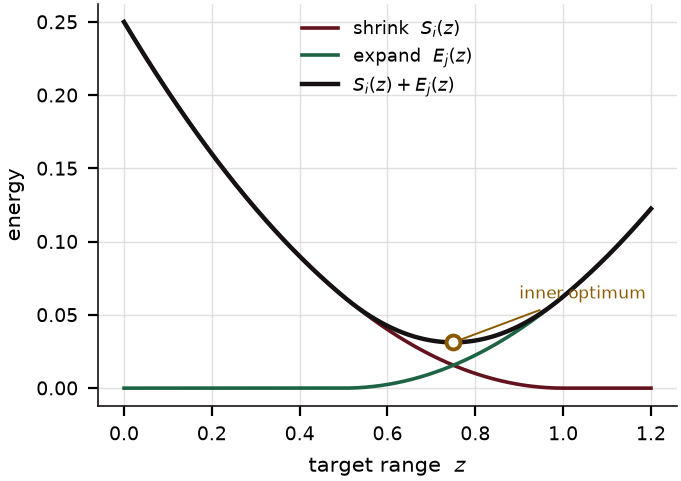
\includegraphics[width=\columnwidth]{func_fig3_shrinkexpand.png}
\caption{Why the inner problem has an interior optimum. Moving the target range costs energy
in two opposing ways: shrinking it below a coordinate's current reach charges $S_{i}(z)$,
which is flat once the range already exceeds $C_{i}$ and then grows quadratically; expanding
it past another coordinate charges $E_{j}(z)$, flat until $C_{j}$ is passed and quadratic
thereafter. Neither term alone has an interior minimum---each is monotone where it is not
flat---but their sum does, marked, because the flat regions do not overlap. This is the
mechanism behind the closed form of Section~\ref{sec:fn-innerqp}, and the reason the optimum is
not simply one of the two endpoints. Exact evaluation of the two energies at
$C_{i}=1$, $C_{j}=\tfrac12$.}
\label{fig:fn-shrinkexpand}
\end{figure}

\subsection{The Certificate, Without an Inverse}
\label{sec:fn-kkt}

\begin{theorem}[KKT sufficiency under semidefiniteness]
\label{thm:fn-kkt}
Let $M$ be symmetric positive semidefinite, $A$ the constraint matrix of a pair region, and
suppose $\lambda^{*}$ and $y$ satisfy
\begin{equation}
M(\lambda^{*}-\mu)+A^{\top}y=0,\quad
y\geq 0,\quad
A\lambda^{*}\leq 0,\quad
y^{\top}A\lambda^{*}=0 .
\label{eq:fn-kkt}
\end{equation}
Then $\lambda^{*}$ minimises the energy over the region.
\end{theorem}

\begin{proof}
Let $\lambda$ be feasible and $d=\lambda-\lambda^{*}$. Expanding,
\begin{align}
&\tfrac12(\lambda-\mu)^{\top}M(\lambda-\mu)
 -\tfrac12(\lambda^{*}-\mu)^{\top}M(\lambda^{*}-\mu) \notag\\
&\qquad=\;d^{\top}M(\lambda^{*}-\mu)\;+\;\tfrac12 d^{\top}Md .
\end{align}
By stationarity $M(\lambda^{*}-\mu)=-A^{\top}y$, so the cross term is
$-y^{\top}A\lambda+y^{\top}A\lambda^{*}=-y^{\top}A\lambda$ using complementary slackness,
which is non-negative since $A\lambda\le0$ and $y\ge0$. The remaining term is non-negative by
positive semidefiniteness.
\end{proof}

\leanbox{\lean{kkt\_certificate}, \lean{certificate\_gives\_lower\_bound} in
\lean{LeanFunctionalRangeDesignCertificateV1}}

No inverse appears anywhere in the proof, and this is why the statement is arranged as
sufficiency rather than as a dual. It matters operationally: an allocator that has learned
something concentrates its budget, so its information matrix loses rank, and a certificate
requiring $M^{-1}$ fails exactly when the allocator is working well.

\subsection{The Two Families}
\label{sec:fn-families}

Both families have two relations and three actions, with Top-1 claimed for relation $i$ and a
parameter $0<\eta\le1$. They share the same capacities $C_{i}=1$, $C_{j}=\tfrac12$ and hence
the same gap; they differ only in which cell carries the small precision $\eta$ and whether
that cell is currently extremal.

\begin{theorem}[Family 1: the proxy overstates]
\label{thm:fn-family1}
Take
\begin{align}
\theta_{i}=(0,1,\tfrac12),\;\alpha_{i}=(1,1,1);\\
\theta_{j}=(0,\tfrac12,\tfrac14),\;\alpha_{j}=(1,1,\eta).
\end{align}
Then $J_{\mathrm{scalar}}=\tfrac{1}{32}$ while
\begin{equation}
0\;\leq\;\frac{J_{\mathrm{full}}}{J_{\mathrm{scalar}}}\;\leq\;9\eta
\;\xrightarrow[\eta\to0]{}\;0 .
\label{eq:fn-family1}
\end{equation}
\end{theorem}

\begin{proof}
Raising \emph{only} the third cell of $j$ from $\tfrac14$ to $1$ equalises the capacities:
$C_{j}$ becomes $1-0=1=C_{i}$. That move costs
$\tfrac12\eta(1-\tfrac14)^{2}=\tfrac{9\eta}{32}$, so
$J_{\mathrm{full}}\le\tfrac{9\eta}{32}$. The proxy, computed at $j$'s current extrema---cells
$2$ and $1$, both at precision $1$---reports $\tfrac{1}{32}$.
\end{proof}

\leanbox{\lean{scalar\_not\_upper\_to\_any\_constant} in
\lean{LeanFunctionalScalarProxyFailsV1}}

The mechanism is that the cheap route to raising $j$'s capacity runs through a cell that is
\emph{not} currently an extremum, and \eqref{eq:fn-scalar} cannot see it because it has frozen
the extrema. As $\eta\to0$ that cell becomes arbitrarily cheap and the true value collapses
while the proxy does not move at all.

\begin{theorem}[Family 2: the proxy understates]
\label{thm:fn-family2}
Take
\begin{align}
\theta_{i}=(0,1,\tfrac34),\;\alpha_{i}=(1,\eta,1);\\
\theta_{j}=(0,\tfrac12,\tfrac14),\;\alpha_{j}=(1,1,1).
\end{align}
Then $J_{\mathrm{full}}\ge\tfrac{1}{128}$ while
\begin{equation}
\frac{J_{\mathrm{full}}}{J_{\mathrm{scalar}}}
\;\geq\;\frac{1+3\eta}{16\eta}
\;\xrightarrow[\eta\to0]{}\;+\infty .
\label{eq:fn-family2}
\end{equation}
\end{theorem}

\begin{proof}
Let $\lambda$ be \emph{any} capacity-inverting alternative and pick $z$ strictly between the
two new capacities. Shrinking $i$ below $z$ costs at least $[\tfrac34-z]_{+}^{2}/4$ by
Theorem~\ref{thm:fn-shrink}; opening $j$ above $z$ costs at least $[z-\tfrac12]_{+}^{2}/4$ by
Theorem~\ref{thm:fn-expand}. By Lemma~\ref{lem:fn-posparts} the two positive parts sum to at least
$\tfrac14$, so $J_{\mathrm{full}}\ge\tfrac14\cdot\tfrac{1}{32}=\tfrac{1}{128}$. The proxy,
seeing $i$'s cheap cell at precision $\eta$, reports $\eta/(8(1+3\eta))$.
\end{proof}

\leanbox{\lean{scalar\_not\_lower\_to\_any\_constant}, \lean{family2\_full\_ge} in
\lean{LeanFunctionalScalarProxyFailsV1}}

\begin{lemma}[Positive parts]
\label{lem:fn-posparts}
For every $z\in\mathbb{R}$,
$\bigl[\tfrac34-z\bigr]_{+}+\bigl[z-\tfrac12\bigr]_{+}\ge\tfrac14$.
\end{lemma}

\begin{proof}
Three cases. If $z\le\tfrac12$ the first part is at least $\tfrac14$; if $z\ge\tfrac34$ the
second is; and in between both are positive and sum to exactly $\tfrac14$.
\end{proof}

\leanbox{\lean{positive\_parts\_sum} in \lean{LeanFunctionalScalarProxyFailsV1}}

\noindent\emph{Supporting results in \lean{LeanFunctionalScalarProxyFailsV1}.}~These are the two counterexamples, and the division of labour matters. The capacity and cost statements evaluate the instances exactly; the two \lean{\_full} statements bound the true value, one above by an exhibited alternative and one below by the positive-parts inequality; the two \lean{\_scalar\_value} statements evaluate \eqref{eq:fn-scalar}; and the two ratio statements combine them. Only then do the two \lean{\_to\_any\_constant} theorems quantify over every positive constant. They are reproduced as the prover has them; a further $4$ audited declarations in this module are positivity checks and measurability side conditions and are not displayed.

\noindent\textbf{S\,22}\quad\lean{cap\_i1}
{\footnotesize\[ \vdash\; \mathit{cap3} 0 1 (1/2) = 1 \]}

\noindent\textbf{S\,23}\quad\lean{cap\_j1}
{\footnotesize\[ \vdash\; \mathit{cap3} 0 (1/2) (1/4) = 1/2 \]}

\noindent\textbf{S\,24}\quad\lean{family1\_alt\_cost}
{\footnotesize\[ (\mathit{eta} : \mathbb{R} ) \;\vdash\; (1/2) * \mathit{eta} * (1 - 1/4) ^{2} = 9 * \mathit{eta} / 32 \]}

\noindent\textbf{S\,25}\quad\lean{family1\_alt\_ties}
{\footnotesize\[ \vdash\; \mathit{cap3} 0 (1/2) 1 = \mathit{cap3} 0 1 (1/2) \]}

\noindent\textbf{S\,26}\quad\lean{family1\_full\_le}
{\footnotesize\[ \begin{aligned}[t]
&(\mathit{Jfull} \mathit{eta} : \mathbb{R} ),\; (\mathit{halt} : \mathit{Jfull} \leq (1/2) * \mathit{eta} * (1 - 1/4) ^{2})\\
\vdash\;&\mathit{Jfull} \leq 9 * \mathit{eta} / 32
\end{aligned} \]}

\noindent\textbf{S\,27}\quad\lean{family1\_scalar\_value}
{\footnotesize\[ \vdash\; (1/2 : \mathbb{R} ) ^{2} / (2 * (1 + 1 + 1 + 1)) = 1 / 32 \]}

\noindent\textbf{S\,28}\quad\lean{family2\_full\_ge}
{\footnotesize\[ \begin{aligned}[t]
&(\mathit{z} : \mathbb{R} )\\
\vdash\;&(1/128 : \mathbb{R} ) \leq (\mathit{max} (3/4 - \mathit{z}) 0) ^{2} / 4 + (\mathit{max} (\mathit{z} - 1/2) 0) ^{2} / 4
\end{aligned} \]}

\noindent\textbf{S\,29}\quad\lean{positive\_parts\_sum}
{\footnotesize\[ (\mathit{z} : \mathbb{R} ) \;\vdash\; (1/4 : \mathbb{R} ) \leq \mathit{max} (3/4 - \mathit{z}) 0 + \mathit{max} (\mathit{z} - 1/2) 0 \]}

\noindent\textbf{S\,30}\quad\lean{scalar\_not\_lower\_to\_any\_constant}
{\footnotesize\[ \begin{aligned}[t]
&(\mathit{C} : \mathbb{R} ),\; (\mathit{hC} : 0 < \mathit{C})\\
\vdash\;&\exists \mathit{eta} : \mathbb{R} , 0 < \mathit{eta} \wedge \mathit{eta} \leq 1 \wedge \mathit{C} * (\mathit{eta} / (8 * (1 + 3 * \mathit{eta}))\\
&\quad ) < (1 / 128 : \mathbb{R} )
\end{aligned} \]}

\noindent\textbf{S\,31}\quad\lean{scalar\_not\_upper\_to\_any\_constant}
{\footnotesize\[ \begin{aligned}[t]
&(\mathit{C} : \mathbb{R} ),\; (\mathit{hC} : 0 < \mathit{C})\\
\vdash\;&\exists \mathit{eta} : \mathbb{R} , 0 < \mathit{eta} \wedge \mathit{eta} \leq 1 \wedge 9 * \mathit{eta} / 32 <\\
&\quad (1 / 32 : \mathbb{R} ) / \mathit{C}
\end{aligned} \]}


Lemma~\ref{lem:fn-posparts} is what closes the quantifier. Without it one could only say that
\emph{some} alternatives are expensive; with it, \emph{every} capacity-inverting alternative
is, whatever $z$ it chooses, so the bound is a property of the instance rather than of a
competitor. Here the mechanism is the reverse of family~1: the proxy sees a cheap route---move
$i$'s second cell at precision $\eta$---and concludes the alternative is nearly free, but
moving that cell alone does not invert the capacities, because $i$'s range is pinned by its
first and third cells.

\begin{corollary}[No constant repairs the proxy]
\label{cor:fn-noconstant}
There is no constant $c$ with $J_{\mathrm{full}}\le c\,J_{\mathrm{scalar}}$ for all
instances, and none with $J_{\mathrm{full}}\ge c\,J_{\mathrm{scalar}}$.
\end{corollary}

\begin{proof}
Family~2 refutes the first for every $c$, taking $\eta$ small enough that
$(1+3\eta)/(16\eta)>c$; family~1 refutes the second.
\end{proof}

\begin{figure}[htbp]
\centering
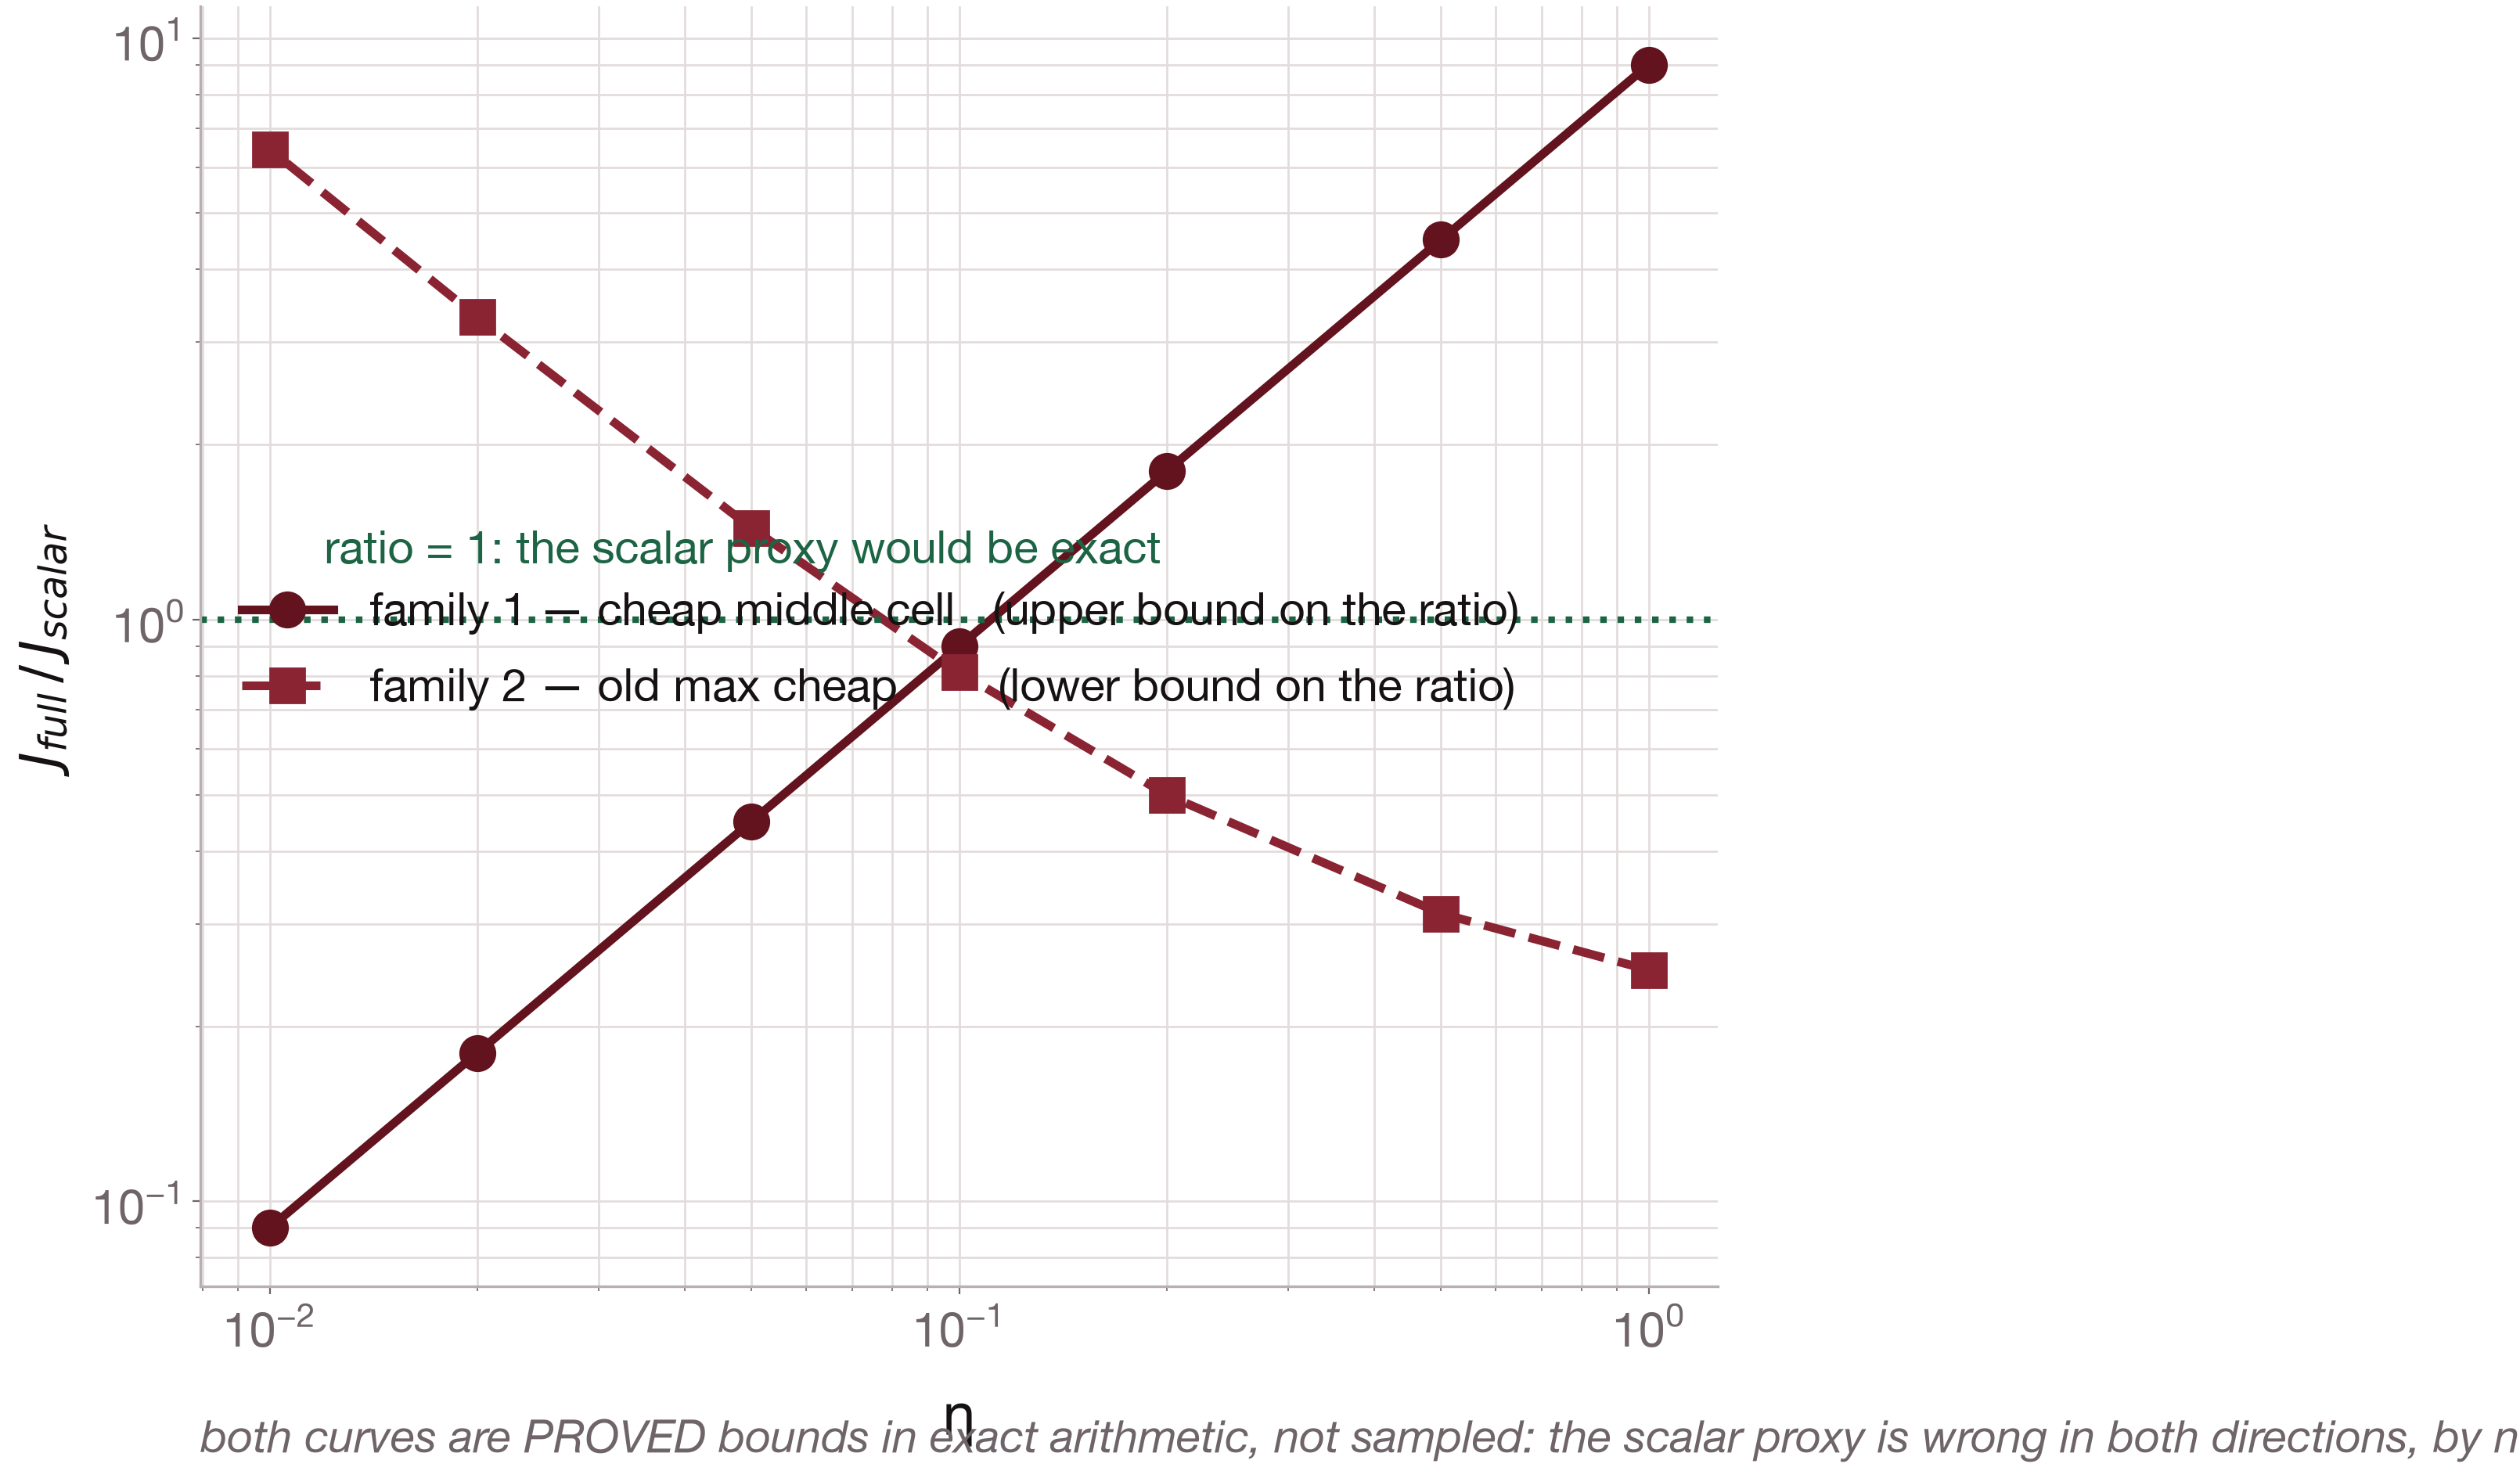
\includegraphics[width=\columnwidth]{func_fig2_families.png}
\caption{The two families. Family~1 forces the ratio below $9\eta$ and family~2 above
$(1+3\eta)/(16\eta)$. Both curves are \emph{proved} bounds in exact arithmetic, not sampled
points, so Corollary~\ref{cor:fn-noconstant} follows from the two envelopes crossing every
horizontal line.}
\label{fig:fn-families}
\end{figure}

\begin{figure}[htbp]
\centering
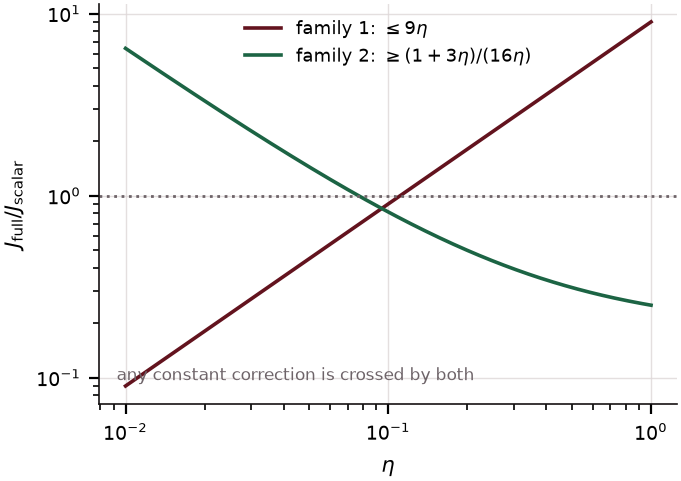
\includegraphics[width=\columnwidth]{func_fig4_ratio.png}
\caption{The two families, on one axis. Family~1 has the full objective within $9\eta$ of the
scalar one, so its ratio to the scalar value goes to $1$ as $\eta\to0$; family~2 has the full
objective at least $(1+3\eta)/(16\eta)$ times the scalar one, so its ratio diverges. Any
proposed correction factor---any constant $c$ claimed to relate the two objectives---is a
horizontal line on this plot, and both curves cross every such line. That is the content of
the separation: the two objectives are not related by a bound in either direction, and no
single-scalar surrogate can be repaired by a constant. Exact evaluation of the two proved
bounds.}
\label{fig:fn-ratio}
\end{figure}

\subsection{Setup Cost and Its Crossing}
\label{sec:fn-setup}

A design that switches support pays a setup cost, and comparing two supports requires knowing
where their budgets cross. A design on support $S$ pays $\kappa|S|$ once and then accrues
value at rate $\Gamma$ per unit of remaining budget, so at total budget $B$ it delivers
$\Gamma(B-\kappa|S|)$, valid while $B\ge\kappa|S|$ and undefined below it.

\begin{theorem}[Crossing budget]
\label{thm:fn-crossing}
With rates $\Gamma_{1}\neq\Gamma_{2}$, support sizes $|S_{1}|,|S_{2}|$ and setup price
$\kappa$,
\begin{equation}
B_{*}\;=\;\kappa\,\frac{|S_{2}|\,\Gamma_{2}-|S_{1}|\,\Gamma_{1}}{\Gamma_{2}-\Gamma_{1}} .
\label{eq:fn-crossing}
\end{equation}
\end{theorem}

\leanbox{\lean{crossing\_budget}, \lean{infeasible\_iff} in
\lean{LeanFunctionalDesignDualityV1} and
\lean{LeanFunctionalRangeDesignCertificateV1}}

Below $B_{*}$ the support with the smaller setup wins even though its rate is worse; above it
the higher rate wins; and the crossing moves linearly in $\kappa$.

\begin{theorem}[Undetermined sign]
\label{thm:fn-undecided}
If $\Gamma_{1}$ and $\Gamma_{2}$ are known only within overlapping brackets, both orders
remain consistent with the data, so the sign of the denominator in \eqref{eq:fn-crossing} is
undetermined and no crossing may be reported.
\end{theorem}

\leanbox{\lean{crossing\_sign\_undetermined} in
\lean{LeanFunctionalRangeDesignCertificateV1}}

\noindent\emph{Supporting results in \lean{LeanFunctionalRangeDesignCertificateV1}.}~These carry the certificate and the setup-cost law. The bilinear and quadratic algebra is separated out so that Theorem~\ref{thm:fn-kkt} uses only symmetry and positive semidefiniteness; the region and single-alternative bounds keep the two directions apart; and the crossing statements include the undetermined-sign result, which is a negative result reported rather than a case left to an implementation. They are reproduced as the prover has them; a further $1$ audited declarations in this module are positivity checks and measurability side conditions and are not displayed.

\noindent\textbf{S\,14}\quad\lean{bil\_symm}
{\footnotesize\[ \begin{aligned}[t]
&(\mathit{M} : \iota \to \iota \to \mathbb{R} ),\; (\mathit{hM} : \forall \mathit{p} \mathit{q}, \mathit{M} \mathit{p} \mathit{q} = \mathit{M} \mathit{q} \mathit{p}),\; (\mathit{x} \mathit{y} : \iota \to \mathbb{R} )\\
\vdash\;&\mathit{bil} \mathit{M} \mathit{x} \mathit{y} = \mathit{bil} \mathit{M} \mathit{y} \mathit{x}
\end{aligned} \]}

\noindent\textbf{S\,15}\quad\lean{certificate\_gives\_lower\_bound}
{\footnotesize\[ \begin{aligned}[t]
&(\mathit{M} : \iota \to \iota \to \mathbb{R} ),\; (\mathit{A} : \kappa \to \iota \to \mathbb{R} ),\; (\mathit{mu} \mathit{lam} : \iota \to \mathbb{R} ),\\
&\quad \; (\mathit{y} : \kappa \to \mathbb{R} ),\; (\mathit{V} : \mathbb{R} ),\; (\mathit{hM} : \forall \mathit{p} \mathit{q}, \mathit{M} \mathit{p} \mathit{q} = \mathit{M} \mathit{q} \mathit{p}),\\
&\quad \; (\mathit{hpsd} : \forall \mathit{d} : \iota \to \mathbb{R} , 0 \leq \mathit{quad} \mathit{M} \mathit{d}),\; (\mathit{hy} : \forall \mathit{c}, 0 \leq \mathit{y} \mathit{c}),\\
&\quad \; (\mathit{hfeas} : \forall \mathit{c}, \mathit{rowAp} \mathit{A} \mathit{lam} \mathit{c} \leq 0),\; (\mathit{hstat} : \forall \mathit{p}, (\textstyle\sum \mathit{q}, \mathit{M} \mathit{p} \mathit{q} * (\mathit{lam} \mathit{q}\\
&\quad - \mathit{mu} \mathit{q})) + (\textstyle\sum \mathit{c}, \mathit{y} \mathit{c} * \mathit{A} \mathit{c} \mathit{p}) = 0),\; (\mathit{hcs} : \textstyle\sum \mathit{c}, \mathit{y} \mathit{c} * \mathit{rowAp} \mathit{A} \mathit{lam} \mathit{c}\\
&\quad = 0),\; (\mathit{hval} : \mathit{V} = (1/2) * \mathit{quad} \mathit{M} (\mathbf{fun} \mathit{p} => \mathit{lam} \mathit{p} - \mathit{mu} \mathit{p}))\\
\vdash\;&\forall \mathit{lam'} : \iota \to \mathbb{R} , (\forall \mathit{c}, \mathit{rowAp} \mathit{A} \mathit{lam'} \mathit{c} \leq 0) \to \mathit{V} \leq\\
&\quad (1/2) * \mathit{quad} \mathit{M} (\mathbf{fun} \mathit{p} => \mathit{lam'} \mathit{p} - \mathit{mu} \mathit{p})
\end{aligned} \]}

\noindent\textbf{S\,16}\quad\lean{crossing\_budget}
{\footnotesize\[ \begin{aligned}[t]
&(\mathit{kappa} \mathit{G1} \mathit{G2} : \mathbb{R} ),\; (\mathit{n1} \mathit{n2} : \mathbb{N} ),\; (\mathit{hne} : \mathit{G2} - \mathit{G1} \neq 0)\\
\vdash\;&\mathit{information} (\mathit{kappa} * ((\mathit{n2} : \mathbb{R} ) * \mathit{G2} - (\mathit{n1} : \mathbb{R} ) * \mathit{G1}) / (\mathit{G2}\\
&\quad - \mathit{G1})) \mathit{kappa} \mathit{n1} \mathit{G1} = \mathit{information} (\mathit{kappa} * ((\mathit{n2} : \mathbb{R} ) * \mathit{G2} - (\\
&\quad \mathit{n1} : \mathbb{R} ) * \mathit{G1}) / (\mathit{G2} - \mathit{G1})) \mathit{kappa} \mathit{n2} \mathit{G2}
\end{aligned} \]}

\noindent\textbf{S\,17}\quad\lean{crossing\_sign\_undetermined}
{\footnotesize\[ \begin{aligned}[t]
&(\mathit{G1lo} \mathit{G1hi} \mathit{G2lo} \mathit{G2hi} : \mathbb{R} ),\; (\mathit{h1} : \mathit{G1lo} \leq \mathit{G1hi}),\\
&\quad \; (\mathit{h2} : \mathit{G2lo} \leq \mathit{G2hi}),\; (\mathit{hov1} : \mathit{G2lo} \leq \mathit{G1hi}),\; (\mathit{hov2} : \mathit{G1lo} \leq\\
&\quad \mathit{G2hi})\\
\vdash\;&(\exists \mathit{g1} \mathit{g2} : \mathbb{R} , \mathit{G1lo} \leq \mathit{g1} \wedge \mathit{g1} \leq \mathit{G1hi} \wedge \mathit{G2lo} \leq \mathit{g2} \wedge \mathit{g2} \leq\\
&\quad \mathit{G2hi} \wedge \mathit{g2} \leq \mathit{g1}) \wedge (\exists \mathit{g1} \mathit{g2} : \mathbb{R} , \mathit{G1lo} \leq \mathit{g1} \wedge \mathit{g1} \leq \mathit{G1hi} \wedge\\
&\quad \mathit{G2lo} \leq \mathit{g2} \wedge \mathit{g2} \leq \mathit{G2hi} \wedge \mathit{g1} \leq \mathit{g2})
\end{aligned} \]}

\noindent\textbf{S\,18}\quad\lean{kkt\_certificate}
{\footnotesize\[ \begin{aligned}[t]
&(\mathit{M} : \iota \to \iota \to \mathbb{R} ),\; (\mathit{A} : \kappa \to \iota \to \mathbb{R} ),\; (\mathit{mu} \mathit{lam} : \iota \to \mathbb{R} ),\\
&\quad \; (\mathit{y} : \kappa \to \mathbb{R} ),\; (\mathit{hM} : \forall \mathit{p} \mathit{q}, \mathit{M} \mathit{p} \mathit{q} = \mathit{M} \mathit{q} \mathit{p}),\; (\mathit{hpsd} : \forall \mathit{d} : \iota \to \mathbb{R} , 0\\
&\quad \leq \mathit{quad} \mathit{M} \mathit{d}),\; (\mathit{hy} : \forall \mathit{c}, 0 \leq \mathit{y} \mathit{c}),\; (\mathit{hfeas} : \forall \mathit{c}, \mathit{rowAp} \mathit{A} \mathit{lam} \mathit{c} \leq\\
&\quad 0),\; (\mathit{hstat} : \forall \mathit{p}, (\textstyle\sum \mathit{q}, \mathit{M} \mathit{p} \mathit{q} * (\mathit{lam} \mathit{q} - \mathit{mu} \mathit{q})) + (\textstyle\sum \mathit{c}, \mathit{y} \mathit{c} * \mathit{A} \mathit{c} \mathit{p})\\
&\quad = 0),\; (\mathit{hcs} : \textstyle\sum \mathit{c}, \mathit{y} \mathit{c} * \mathit{rowAp} \mathit{A} \mathit{lam} \mathit{c} = 0),\; (\mathit{lam'} : \iota \to \mathbb{R} ),\\
&\quad \; (\mathit{hfeas'} : \forall \mathit{c}, \mathit{rowAp} \mathit{A} \mathit{lam'} \mathit{c} \leq 0)\\
\vdash\;&(1/2) * \mathit{quad} \mathit{M} (\mathbf{fun} \mathit{p} => \mathit{lam} \mathit{p} - \mathit{mu} \mathit{p}) \leq (1/2) * \mathit{quad} \mathit{M} (\\
&\quad \mathbf{fun} \mathit{p} => \mathit{lam'} \mathit{p} - \mathit{mu} \mathit{p})
\end{aligned} \]}

\noindent\textbf{S\,19}\quad\lean{quad\_add}
{\footnotesize\[ \begin{aligned}[t]
&(\mathit{M} : \iota \to \iota \to \mathbb{R} ),\; (\mathit{hM} : \forall \mathit{p} \mathit{q}, \mathit{M} \mathit{p} \mathit{q} = \mathit{M} \mathit{q} \mathit{p}),\; (\mathit{a} \mathit{d} : \iota \to \mathbb{R} )\\
\vdash\;&\mathit{quad} \mathit{M} (\mathit{a} + \mathit{d}) = \mathit{quad} \mathit{M} \mathit{a} + 2 * \mathit{bil} \mathit{M} \mathit{d} \mathit{a} + \mathit{quad} \mathit{M} \mathit{d}
\end{aligned} \]}

\noindent\textbf{S\,20}\quad\lean{region\_min\_lower\_bounds\_J}
{\footnotesize\[ \begin{aligned}[t]
&(\mathit{R} : \mathit{Finset} \rho ),\; (\mathit{hR} : \mathit{R}.\mathit{Nonempty}),\; (\mathit{cost} : \rho \to \mathbb{R} ),\; (\mathit{J} : \mathbb{R} ),\\
&\quad \; (\mathit{hJ} : \mathit{J} = \mathit{R}.\mathit{inf'} \mathit{hR} \mathit{cost}),\; (\mathit{b} : \rho \to \mathbb{R} ),\; (\mathit{hb} : \forall \mathit{r} \in \mathit{R}, \mathit{b} \mathit{r} \leq\\
&\quad \mathit{cost} \mathit{r})\\
\vdash\;&\mathit{R}.\mathit{inf'} \mathit{hR} \mathit{b} \leq \mathit{J}
\end{aligned} \]}

\noindent\textbf{S\,21}\quad\lean{single\_alt\_upper}
{\footnotesize\[ \begin{aligned}[t]
&(\mathit{R} : \mathit{Finset} \rho ),\; (\mathit{hR} : \mathit{R}.\mathit{Nonempty}),\; (\mathit{cost} : \rho \to \mathbb{R} ),\; (\mathit{J} : \mathbb{R} ),\\
&\quad \; (\mathit{hJ} : \mathit{J} = \mathit{R}.\mathit{inf'} \mathit{hR} \mathit{cost}),\; \{ \mathit{r} : \rho \},\; (\mathit{hr} : \mathit{r} \in \mathit{R})\\
\vdash\;&\mathit{J} \leq \mathit{cost} \mathit{r}
\end{aligned} \]}


This negative result is stated deliberately. A procedure that substitutes bracket midpoints
into \eqref{eq:fn-crossing} will report not merely an imprecise crossing but one pointing the
wrong way; the failure is qualitative. The same discipline governs infeasibility: a
configuration in which no alternative inverts the capacities has \emph{no} finite value, and
returning a small number for it would tell an allocator the answer is about to flip when it
cannot. Three outcomes---a value, \textsc{infeasible}, \textsc{undecided}---are therefore
distinguished throughout rather than encoded in a sentinel number.

\begin{theorem}[Break-even, without the folklore 4]
\label{thm:fn-breakeven}
$\min_{p}\bigl[\sigma_{a}^{2}/p+\sigma_{b}^{2}/(1-p)\bigr]=(\sigma_{a}+\sigma_{b})^{2}$, so
break-even occurs at $c_{c}\nu_{c}=(\sigma_{a}+\sigma_{b})^{2}$.
\end{theorem}

\leanbox{\lean{scalar\_split\_optimal}, \lean{breakeven\_iff}, \lean{breakeven\_not\_four}
in \lean{LeanFunctionalDesignDualityV1}}

\noindent\emph{Supporting results in \lean{LeanFunctionalDesignDualityV1}.}~These are the duality side. Weak duality and the dual certificate are proved, and the infeasibility characterisation is stated so that an empty feasible set returns \textsc{infeasible} rather than a small number. The break-even group is included because the constant $4$ that circulates as a threshold is the value of $(\sigma_{a}+\sigma_{b})^{2}$ at unit variances and nothing more. They are reproduced as the prover has them; a further $6$ audited declarations in this module are positivity checks and measurability side conditions and are not displayed.

\noindent\textbf{S\,32}\quad\lean{design\_value\_ge}
{\footnotesize\[ \begin{aligned}[t]
&(\mathit{Q} : \mathit{Finset} \iota ),\; (\mathit{hQ} : \mathit{Q}.\mathit{Nonempty}),\; (\mathit{f} : \iota \to \mathit{W} \to \mathbb{R} ),\; (\mathit{w} : \mathit{W}),\\
&\quad \; (\mathit{c} : \mathbb{R} ),\; (\mathit{h} : \forall \mathit{q} \in \mathit{Q}, \mathit{c} \leq \mathit{f} \mathit{q} \mathit{w})\\
\vdash\;&\mathit{c} \leq \mathit{designValue} \mathit{Q} \mathit{hQ} \mathit{f} \mathit{w}
\end{aligned} \]}

\noindent\textbf{S\,33}\quad\lean{design\_value\_le}
{\footnotesize\[ \begin{aligned}[t]
&(\mathit{Q} : \mathit{Finset} \iota ),\; (\mathit{hQ} : \mathit{Q}.\mathit{Nonempty}),\; (\mathit{f} : \iota \to \mathit{W} \to \mathbb{R} ),\; (\mathit{w} : \mathit{W}),\\
&\quad \; \{ \mathit{q} : \iota \},\; (\mathit{hq} : \mathit{q} \in \mathit{Q})\\
\vdash\;&\mathit{designValue} \mathit{Q} \mathit{hQ} \mathit{f} \mathit{w} \leq \mathit{f} \mathit{q} \mathit{w}
\end{aligned} \]}

\noindent\textbf{S\,34}\quad\lean{dual\_gap\_zero}
{\footnotesize\[ \begin{aligned}[t]
&(\mathit{Q} : \mathit{Finset} \iota ),\; (\mathit{hQ} : \mathit{Q}.\mathit{Nonempty}),\; (\mathit{f} : \iota \to \mathit{W} \to \mathbb{R} ),\\
&\quad \; (\mathit{lam} : \iota \to \mathbb{R} ),\; (\mathit{hlam} : \forall \mathit{q} \in \mathit{Q}, 0 \leq \mathit{lam} \mathit{q}),\; (\mathit{hsum} : \textstyle\sum \mathit{q} \in \mathit{Q},\\
&\quad \mathit{lam} \mathit{q} = 1),\; (\mathit{U} : \mathbb{R} ),\; (\mathit{w₀} : \mathit{W}),\; (\mathit{hcert} : \forall \mathit{w} : \mathit{W}, \textstyle\sum \mathit{q} \in \mathit{Q},\\
&\quad \mathit{lam} \mathit{q} * \mathit{f} \mathit{q} \mathit{w} \leq \mathit{U}),\; (\mathit{hattain} : \mathit{designValue} \mathit{Q} \mathit{hQ} \mathit{f} \mathit{w₀} = \mathit{U})\\
\vdash\;&\mathit{IsGreatest} \{ \mathit{v} | \exists \mathit{w} : \mathit{W}, \mathit{designValue} \mathit{Q} \mathit{hQ} \mathit{f} \mathit{w} = \mathit{v}\} \mathit{U}
\end{aligned} \]}

\noindent\textbf{S\,35}\quad\lean{infeasible\_iff}
{\footnotesize\[ \begin{aligned}[t]
&(\mathit{total} \mathit{setup} : \mathbb{R} ),\; (\mathit{channels} : \mathbb{N} )\\
\vdash\;&\mathit{sampleBudget} \mathit{total} \mathit{setup} \mathit{channels} = \mathit{none} \leftrightarrow \mathit{total} <\\
&\quad \mathit{setup} * (\mathit{channels} : \mathbb{R} )
\end{aligned} \]}

\noindent\textbf{S\,36}\quad\lean{information\_of\_budget}
{\footnotesize\[ \begin{aligned}[t]
&(\mathit{total} \mathit{setup} \mathit{unit} : \mathbb{R} ),\; (\mathit{channels} : \mathbb{N} ),\; (\mathit{h} : \mathit{setup} * (\\
&\quad \mathit{channels} : \mathbb{R} ) \leq \mathit{total}),\; (\mathit{hsetup} : 0 \leq \mathit{setup}),\; (\mathit{hunit} : 0 \leq\\
&\quad \mathit{unit})\\
\vdash\;&0 \leq (\mathit{total} - \mathit{setup} * (\mathit{channels} : \mathbb{R} )) * \mathit{unit} \wedge\\
&\quad (\mathit{total} - \mathit{setup} * (\mathit{channels} : \mathbb{R} )) * \mathit{unit} \leq \mathit{total} * \mathit{unit}
\end{aligned} \]}

\noindent\textbf{S\,37}\quad\lean{value\_of\_feasible}
{\footnotesize\[ \begin{aligned}[t]
&(\mathit{total} \mathit{setup} : \mathbb{R} ),\; (\mathit{channels} : \mathbb{N} ),\; (\mathit{h} : \mathit{setup} * (\mathit{channels} :\\
&\quad \mathbb{R} ) \leq \mathit{total})\\
\vdash\;&\mathit{sampleBudget} \mathit{total} \mathit{setup} \mathit{channels} = \mathit{some} (\mathit{total} - \mathit{setup} * (\\
&\quad \mathit{channels} : \mathbb{R} ))
\end{aligned} \]}


The number $4$ that circulates as a break-even threshold is the value of
$(\sigma_{a}+\sigma_{b})^{2}$ at unit variances and nothing more. With several alternatives
the scalar design shares cells and the pairwise threshold does not transfer.

\subsection{The Oracle as a Procedure}
\label{sec:fn-procedure}

\begin{algorithm}[htbp]
\caption{Exact certification energy}
\label{alg:fn-oracle}
\begin{algorithmic}[1]
\FOR{each $i\in T$, $j\notin T$, ordered pair $(a,b)$ of $j$'s actions}
  \STATE Form the region $\mathcal{P}_{ijab}$ of \eqref{eq:fn-polyhedron}
         \COMMENT{covers the alternative set exactly, Thm~\ref{thm:fn-union}}
  \STATE Evaluate $\inf_{z\ge0}\bigl[S_{i}(z)+E_{j}(z)\bigr]$ using
         \eqref{eq:fn-shrink} and \eqref{eq:fn-expand}
  \STATE Where one cell pair moves per relation, read the value from
         \eqref{eq:fn-innerqp} directly
  \STATE Certify the minimiser by \eqref{eq:fn-kkt} \COMMENT{valid for singular $M$}
\ENDFOR
\STATE \textbf{return} the minimum over the index set
       \COMMENT{is the oracle value, Thm~\ref{thm:fn-oracle}}
\end{algorithmic}
\end{algorithm}

The index set has size $|T|\cdot|T^{c}|\cdot|A|(|A|-1)$, polynomial in the problem size and
independent of any discretisation, and each piece is either a closed form or a
one-dimensional minimisation over $z$ whose integrand is a sum of two explicit convex
functions. The contrast with \eqref{eq:fn-scalar} is therefore not that the exact oracle is
intractable and the proxy cheap; it is that the exact oracle is a finite enumeration of
closed forms and the proxy is one of them evaluated at the wrong index.


\section{Experimental Design}

\subsection{Certified Compression Under a Known Margin}
\label{sec:d6-expdesign}

\subsection{Experimental Objectives}

The theorems quantify over all parameters, so the numerical work cannot strengthen them. It
has two objectives. The first is to confirm that the derived weights agree with the previously
fitted ones on the cells where the fit was performed, which is a check on the implementation.
The second concerns a hypothesis rather than an implementation. The sufficiency half of the
threshold, Theorem~\ref{thm:d6-sufficient}, is proved for an arbitrary product reference; the
necessity half, Theorem~\ref{thm:d6-subthreshold}, is proved at the corner reference only.
Nothing in the formal development says what happens between them, and the honest question is
not whether the witness survives an arbitrary reference---it is not claimed to---but how far
from the corner it survives, and whether the failure is abrupt or gradual. Experiment~E2
measures that.

\subsection{Setup}

The design grid is $q\in\{8,16\}$, $\mu\in\{\tfrac14,\tfrac25\}$, $c\in\{\tfrac32,2\}$ and
$\eta\in\{\tfrac13,\tfrac{13}{20},\tfrac45\}$, giving $24$ cells. The separation certificate
is evaluated on eight cells, and the pair-query necessity test on twenty.

\subsection{E2: The Reference Sweep}
\label{sec:d6-e2}

The reference is moved off the corner along the one-parameter product family
$q_{i}(\mathrm{true})=t$, which places mass $t$ on the true response in every coordinate
independently and recovers the corner at $t=0$. The grid is the seventeen rationals
$t=0,\tfrac1{32},\dots,\tfrac12$, crossed with two dimensions $n\in\{6,8\}$ and five margins
$\rho\in\{1,\tfrac54,\tfrac32,\tfrac74,2\}$---one hundred and seventy cells, of which one
hundred and sixty have $t>0$.

\begin{algorithm}[htbp]
\caption{Evaluating the construction under one reference}
\label{alg:d6-sweep}
\begin{algorithmic}[1]
\REQUIRE dimension $n$, selected set $A$, steered coordinate $j\notin A$, margin $\mu$,
         product reference $q_{i}(\mathrm{true})=t_{i}$
\ENSURE whether $A$ is still a Top-$C$ set, and the doubled regret against its complement
\STATE $F(x)\leftarrow\textsc{Steered}(A,j,\mu)(x)$ for every $x\in\{0,1\}^{n}$
       \COMMENT{independent of the reference, so tabulated once per configuration and
       reused across every $t$ --- this is what makes the wide sweep affordable}
\STATE $W(c)\leftarrow\prod_{i}\bigl(t_{i}\text{ if }c_{i}\text{ else }1-t_{i}\bigr)$
\FORALL{coordinates $i$ and values $u\in\{0,1\}$}
  \STATE $Q_{i}(u)\leftarrow\sum_{c}W(c)\,F(c\text{ with }c_{i}:=u)$
\ENDFOR
\STATE $\mathrm{osc}_{i}\leftarrow|Q_{i}(1)-Q_{i}(0)|$;
       $\;T\leftarrow$ the $|A|$ coordinates of largest $\mathrm{osc}$
\STATE $L(S)\leftarrow\tfrac12\bigl(\max_{x}-\min_{x}\bigr)
       \bigl[F(x)-\sum_{i\in S}Q_{i}(x_{i})\bigr]$
\RETURN $\bigl[T=A\bigr]$ and $2\bigl(L(A)-L(A^{\complement})\bigr)$
\end{algorithmic}
\end{algorithm}

\noindent All of it is exact rational arithmetic, so a reported flip is a flip and not a
rounding artefact. Two properties of the setup matter more than its size. First, every quantity is computed in
exact rational arithmetic, so a reported flip is a flip and not a rounding artefact. Second,
the definitions are not re-derived for the experiment: the gate, the coefficient map, the
steered world and the compression loss are transcribed from the Lean sources, and the
transcription is validated before any sweep result is reported. At $t=0$ the transcription
must reproduce \lean{steered\_span}---oscillation $\rho$ on $A$ and $0$ off it---and
\lean{steered\_exchange\_equality}---doubled regret exactly $|A|(2-\rho)$. It does, in all
nine validation configurations and all ten corner cells. A sweep whose code does not
reproduce the theorems at the one point where the theorems apply is measuring something else,
and this check is what rules that out.

\subsection{E3: Four Axes Instead of One}
\label{sec:d6-e3}

E2 moves the reference along a single symmetric path. That leaves the obvious objection
unanswered: the path is symmetric, the construction is symmetric, and a symmetric
perturbation may be the one direction in which nothing happens. E3 widens the sweep on four
axes at once.

\emph{Dimension.} $n\in\{6,8,10\}$ with $|A|=n/2$. The balance is not a convenience: the
exchange equality carries the hypothesis $|A^{\complement}|=|A|$, so these are the
configurations the theorems speak about. Twelve unbalanced configurations are swept as well,
in a separate arm, precisely because the theorem does not cover them---and nothing there is
checked against it.

\emph{Margin and resolution.} Nine margins from $1$ to $2$ rather than five, on a
sixty-five-point grid in $t$, so the breakdown point is located to $1/64$ and can be traced
against the margin rather than sampled.

\emph{Direction.} This is the axis that answers the objection. Besides the symmetric path,
four structured directions perturb only $A$, only its complement, only the steered coordinate
$j$, or everything but $j$; and two hundred references per configuration are drawn with an
independent $t_{i}$ in each coordinate. If the finding survives an asymmetric reference it is
not an artefact of the symmetric one.

Responses of the steered world do not depend on the reference, so they are tabulated once per
configuration and reused, which is what makes the wider sweep affordable. Both self-checks of
Section~\ref{sec:d6-e2} are re-run at every configuration.

\subsection{Metrics}

For the design experiment: the two derived weights, the budget residual
$w_{B}+c\,w_{\mathrm{pair}}-1$, agreement with the fitted values, the certificate verdict per
cell and which endpoint produced it, and the number of cells in which the pair query carries
positive weight and its necessity is certified.

For E2, three quantities per cell: whether $A$ is still a Top-$C$ set under the perturbed
reference, which is the hypothesis of Theorem~\ref{thm:d6-subthreshold}; the doubled regret
$2(L(A)-L(A^{\complement}))$, which is its conclusion; and the oscillation profile that
explains the two. Reporting the hypothesis and the conclusion separately is deliberate---they
fail at different values of $t$, and a single pass/fail per cell would hide that.

\subsection{Statistical Reporting}

Every quantity in this section is exact rational arithmetic; there is no sampling, no seed and
no confidence interval anywhere in it. E2 is labelled \NUM{} throughout, not because it is
inexact---it is exact---but because it is a finite sweep of a parameter family and supports no
universally quantified claim. No result from it is used to support a \PROVED{} one, and where
it bears on a proved statement, as at $t=0$, it is a check on the transcription rather than
evidence for the theorem.


\subsection{The Geometry of the Alternative, and What a Scalar Proxy Loses}
\label{sec:fn-expdesign}

\subsection{Experimental Objectives}

The two families are proved, so no experiment bears on them. The empirical work has two
objectives. The first is to establish which existing allocator is the baseline that any new
one---including one built on Algorithm~\ref{alg:fn-oracle}---must beat. The second concerns the
separation itself. Theorems~\ref{thm:fn-family1} and \ref{thm:fn-family2} are enough to refute any
constant correction factor, and they are hand-built to do exactly that. They leave the
practitioner's question open: on an instance nobody designed, how often is the scalar proxy
wrong, by how much, and in which direction? Experiment~E2 answers it.

\subsection{E2: The Proxy on Instances Nobody Built}
\label{sec:fn-e2}

\emph{Instances.} Six thousand are drawn from declared ranges: three to eight actions per
relation, responses uniform on $[0,1]$, and precisions log-uniform over three decades. The
relation with the larger capacity is taken as the claimed top, so the comparison is always in
the direction the proxy is used.

\emph{Computing the true value.} $J_{\mathrm{full}}$ is not estimated. Fix a target width
$z$: relation $i$ must fit inside a window of that width, costing $S_{i}(z)$, and relation
$j$ must open some pair to at least that width, costing $E_{j}(z)$. Both are convex in $z$
for a fixed pair, so $J_{\mathrm{full}}=\min_{z}\min_{(c,d)}[S_{i}(z)+E^{(c,d)}_{j}(z)]$ is
computed exactly. $S_{i}(z)$ has its own closed form: its derivative in the window position
is piecewise linear, so the optimal position is a root on one of the intervals between
breakpoints---and, as it happens, generally interior rather than at a breakpoint, which is
where a first implementation of this experiment went wrong and over-estimated the value.

\begin{algorithm}[htbp]
\caption{Exact least energy of a capacity-inverting alternative}
\label{alg:fn-jfull}
\begin{algorithmic}[1]
\REQUIRE responses $\theta_{i},\theta_{j}$ and precisions $\alpha_{i},\alpha_{j}$
\ENSURE $J_{\mathrm{full}}=\min\{\text{energy}:C_{i}(\lambda)\le C_{j}(\lambda)\}$, exactly
\STATE for a target width $z$, relation $i$ must fit inside a window of width $z$ and
       relation $j$ must open some ordered pair to at least $z$; write $z=C_{i}(\lambda)$
\STATE \textbf{shrink cost } $S_{i}(z)$: the optimal row is $\theta_{i}$ clipped into
       $[l,l+z]$, so the cost is a sum of one-sided squared hinges and is convex in $l$; its
       derivative is piecewise linear with breakpoints at $\theta_{i}$ and $\theta_{i}-z$,
       so solve $D(l)=0$ on each interval and keep the root inside it
       \COMMENT{the minimiser is generally \emph{interior}; scanning breakpoints alone
       over-estimates}
\STATE \textbf{expand cost } $E^{(c,d)}_{j}(z)=\tfrac12\bigl[z-(\theta_{jc}-\theta_{jd})\bigr]_{+}^{2}
       \dfrac{\alpha_{jc}\alpha_{jd}}{\alpha_{jc}+\alpha_{jd}}$
       \COMMENT{split the move between the two cells in inverse proportion to precision}
\STATE $S_{i}$ does not depend on the pair, so evaluate it once on a grid of $z$ and add the
       pair costs vectorised
\FORALL{ordered pairs $(c,d)$ of relation $j$}
  \STATE $S_{i}(z)+E^{(c,d)}_{j}(z)$ is convex in $z$, so refine the grid minimum by
         golden section on the bracketing interval
\ENDFOR
\RETURN the least value over all pairs
\end{algorithmic}
\end{algorithm}

\emph{Checking the solver rather than trusting it.} The decomposition is cross-checked
against SLSQP running on the raw variables, which uses none of it. A local optimiser can only
land at or above the true minimum, so a cell where it lands \emph{below} would expose a
defect; those cells are counted rather than averaged away.

\emph{Self-check.} On the two proved families the implementation must reproduce the proved
numbers before the sweep is reported: $J_{\mathrm{scalar}}=\tfrac1{32}$ and
$J_{\mathrm{full}}\le 9\eta/32$ for family~1, and
$J_{\mathrm{scalar}}=\eta/(8(1+3\eta))$ and $J_{\mathrm{full}}\ge\tfrac1{128}$ for family~2.

\emph{Mechanism.} Each instance also records whether the cheapest alternative opens a pair of
$j$ other than its current extrema. That is the mechanism family~1 exploits, and recording it
turns ``the proxy is sometimes wrong'' into a statement about \emph{when}.

\subsection{Setup}

The confirmatory panel is $10$ seeds $\times$ $1{,}000$ instances $\times$ $8$ policies
$=80{,}000$ policy runs at horizon $131{,}072$, drawing $5{,}042{,}978{,}194$ samples in
total, with $29.1\%$ of runs censored at the horizon. It ran as ten parallel processes for
roughly six CPU-hours each.

\subsection{Baselines}

Three policies are reported: $\mathrm{C\_lucb}$, $\mathrm{C\_anytime}$, and uniform
allocation. All three are existing allocators; no allocator built on
Algorithm~\ref{alg:fn-oracle} appears, and Section~\ref{sec:fn-discussion} says so again.

\subsection{Metrics}

The number of instances certified, the certification fraction, and the median query count
among certified runs. Paired per-instance comparisons are reported alongside, since the
policies run on identical instances.

\subsection{Statistical Reporting}

Results are reported over $10$ seeds. Because $29.1\%$ of runs are censored at the horizon,
both the certification fraction and the median are reported: a policy certifying fewer worlds
but faster on those it certifies would look good on median alone.


\section{Formal Verification}

\subsection{Certified Compression Under a Known Margin}
\label{sec:d6-verification}

\subsection{Acceptance Contract}

A module counts as accepted only when all six of the following hold: the compiler exits zero
with no errors; the source hash is unchanged \emph{across} the compile, so the file checked is
the file on disk; the compiled artifact is newer than its source; at least one
\texttt{\#print axioms} directive is present; the axiom set of every audited declaration lies
within $\{\textsf{propext},\textsf{Classical.choice},\textsf{Quot.sound}\}$; and no
\texttt{sorry} appears anywhere in the file.

This contract is shared with the other papers of the programme and is reproduced verbatim in
each, so that no paper's evidence claim has to be read against a different standard; the
wording is common and the counts in this section are not. The contract is stated in full
because each clause excludes a specific way of appearing verified without being so. The hash check across the compile excludes editing a file after
checking it; the artifact-newer check excludes a stale \texttt{.olean}; and the axiom audit is
a \emph{whitelist} rather than a blacklist, so an axiom introduced by a decision procedure
outside the kernel is rejected by name mismatch rather than needing to be anticipated.

\subsection{Evidence per Step}

\begin{table}[htbp]
\caption{Evidence per step. All cited declarations are axiom-audited.}
\label{tab:d6-inventory}
\centering\footnotesize\setlength{\tabcolsep}{3pt}
\begin{tabular}{@{}llr@{}}
\toprule
Step & Module & Aud. \\
\midrule
Slice, Thms~\ref{thm:d6-slice}--\ref{thm:d6-nonblind} & \lean{LeanD6GeneralFamilyV1}       & 5 \\
Design, Thms~\ref{thm:d6-unique}--\ref{thm:d6-affine} & \lean{LeanD6DesignDerivationV1}    & 7 \\
Surplus, Lem~\ref{lem:d6-surplus}                  & \lean{LeanD6MarginSensitiveExchangeV1} & 3 \\
Exchange, Thms~\ref{thm:d6-exchange}--\ref{thm:d6-marginexchange} & \lean{LeanD6MarginSensitiveExchangeV1} & 3 \\
Threshold, Thms~\ref{thm:d6-sufficient}--\ref{thm:d6-subthreshold} & \lean{LeanD6SharpMarginThresholdV1} & 3 \\
Separation, Thm~\ref{thm:d6-modulus}               & \lean{LeanD6AlternativeReductionV1} & 7 \\
\bottomrule
\end{tabular}
\end{table}

\subsection{Scope of the Formalisation}

The D6 strand contains $444$ Lean source files with $4{,}087$ theorem and lemma statements,
of which $30$ modules carry an acceptance receipt covering $187$ audited declarations. Across
the programme: $762$ files, $7{,}199$ statements, $111$ accepted modules, $857$ audited
declarations.

The ratio of strand size to displayed equations invites the question of what the rest is doing,
and the answer is characteristic. Most of the strand is search and refutation: establishing
that the $(d,x)$ family is the right one required first establishing that several other
candidate families were not, and each withdrawn formulation leaves behind the statements that
ruled it out. The separation certificates are issued per cell, so the file count scales with
the parameter grid rather than with mathematical content.
Every audited statement of every module this paper cites is displayed in Section~\ref{sec:d6-setting}, attached to the step that uses it; only positivity checks and measurability side conditions are omitted, and their count is given at each block. The strand contains a further $26$ accepted modules carrying $167$ audited declarations that no step of this paper uses; they belong to other results of the programme. Appendix~\ref{app:d6-inventory} reproduces the complete chain: all $187$ audited statements of the strand across its $30$ accepted modules, grouped by module.


\subsection{The Geometry of the Alternative, and What a Scalar Proxy Loses}
\label{sec:fn-verification}

\subsection{Acceptance Contract}

A module counts as accepted only when all six of the following hold: the compiler exits zero
with no errors; the source hash is unchanged \emph{across} the compile, so the file checked is
the file on disk; the compiled artifact is newer than its source; at least one
\texttt{\#print axioms} directive is present; the axiom set of every audited declaration lies
within $\{\textsf{propext},\textsf{Classical.choice},\textsf{Quot.sound}\}$; and no
\texttt{sorry} appears anywhere in the file.

This contract is shared with the other papers of the programme and is reproduced verbatim in
each, so that no paper's evidence claim has to be read against a different standard; the
wording is common and the counts in this section are not. The contract is stated in full
because each clause excludes a specific way of appearing verified without being so. The hash check across the compile excludes editing a file after
checking it; the artifact-newer check excludes a stale \texttt{.olean}; and the axiom audit is
a \emph{whitelist} rather than a blacklist, so an axiom introduced by a decision procedure
outside the kernel is rejected by name mismatch rather than needing to be anticipated.

\subsection{Evidence per Step}

\begin{table}[htbp]
\caption{Evidence per step. All cited declarations are axiom-audited. Module names are
prefixed \lean{LeanFunctional}, elided for width.}
\label{tab:fn-inventory}
\centering\footnotesize\setlength{\tabcolsep}{3pt}
\begin{tabular}{@{}llr@{}}
\toprule
Step & Module & Aud. \\
\midrule
Union, Thm~\ref{thm:fn-union}              & \lean{...RangeAlternativeUnionV1}  &  7 \\
Oracle, Thm~\ref{thm:fn-oracle}            & \lean{...RangeEnergyOracleV1}      &  5 \\
Shrink/expand, Thms~\ref{thm:fn-shrink}--\ref{thm:fn-expand} & \lean{...ShrinkExpandV1} & 9 \\
Inner QP, Thm~\ref{thm:fn-innerqp}         & \lean{...RangeEnergyOracleV1}      &  5 \\
Certificate, Thm~\ref{thm:fn-kkt}          & \lean{...RangeDesignCertificateV1} &  9 \\
Families, Thms~\ref{thm:fn-family1}--\ref{thm:fn-family2} & \lean{...ScalarProxyFailsV1} & 14 \\
Setup cost, Thms~\ref{thm:fn-crossing}--\ref{thm:fn-undecided} & \lean{...DesignDualityV1} & 21 \\
Break-even, Thm~\ref{thm:fn-breakeven}     & \lean{...DesignDualityV1}          & 12 \\
\bottomrule
\end{tabular}
\end{table}

\subsection{Scope of the Formalisation}

The Functional strand contains $49$ Lean source files with $430$ theorem and lemma
statements, of which $21$ modules carry an acceptance receipt covering $162$ audited
declarations. Across the programme: $762$ files, $7{,}199$ statements, $111$ accepted modules,
$857$ audited declarations.

Three formulations were withdrawn under the prover. The first version of the union identity
froze the extrema at the truth, so the forward direction of Theorem~\ref{thm:fn-union} fails---
precisely the phenomenon family~1 exploits. The expand cost initially minimised over unordered
pairs, which overstates $E_{j}$ by forcing a third cell to move. And the certificate initially
followed the textbook route through $M^{-1}$, which would have propagated an invertibility
hypothesis into every downstream statement. Every audited statement of every module this paper cites is displayed in Section~
ef{sec:setting}, attached to the step that uses it; only positivity checks and measurability side conditions are omitted, and their count is given at each block. The strand contains a further $15$ accepted modules carrying $106$ audited declarations that no step of this paper uses; they belong to other results of the programme. Appendix~\ref{app:fn-inventory} reproduces the complete chain: all $162$ audited statements of the strand across its $21$ accepted modules, grouped by module.


\section{Results}

\subsection{Certified Compression Under a Known Margin}
\label{sec:d6-results}

\subsection{Reporting Protocol}

All $24$ cells are reported with no exclusions.

\subsection{The Derived Weights Match All 24 Cells Exactly}

The previously fitted weights agree with \eqref{eq:d6-design} in every cell, and the budget
identity holds exactly in each. The weights vary with $(\eta,c)$ and are constant across
$(q,\mu)$, exactly as Corollary~\ref{cor:d6-indep} predicts.

The logical status of the table changed with Section~\ref{sec:d6-design}. Before the derivation
it was the evidence---$24$ consistent cells, suggestive but not conclusive, licensing no
prediction at a $25$th cell. After it, the table is a check on the arithmetic: the theorem
says the agreement must hold at every $(q,\mu,c,\eta)$, so a disagreeing cell would now be an
implementation bug rather than a puzzle.

\subsection{The Separation Is Certified on Every Cell Tested}

Eight of eight cells certify the strict separation across the whole cell, all by the
left-endpoint test of \eqref{eq:d6-modulus}, with exact rational gaps. That every certificate
came from the same endpoint is itself informative: the modulus decays across the cell, so the
binding case is the left edge, and a procedure testing the midpoint would have been testing
the easy case.

\subsection{The Pair Query Is Necessary Wherever It Is Used}

On $20$ parameter cells the pair query carries positive weight in $17$, and in all $17$ its
necessity is certified: the full value strictly exceeds the best value achievable without it.
The three cells without a certificate are exactly those where the pair weight is zero. The
coincidence of those two sets is the point---a missing certificate indicates a cell where the
query is unused, not one where the argument failed.

\begin{figure}[htbp]
\centering
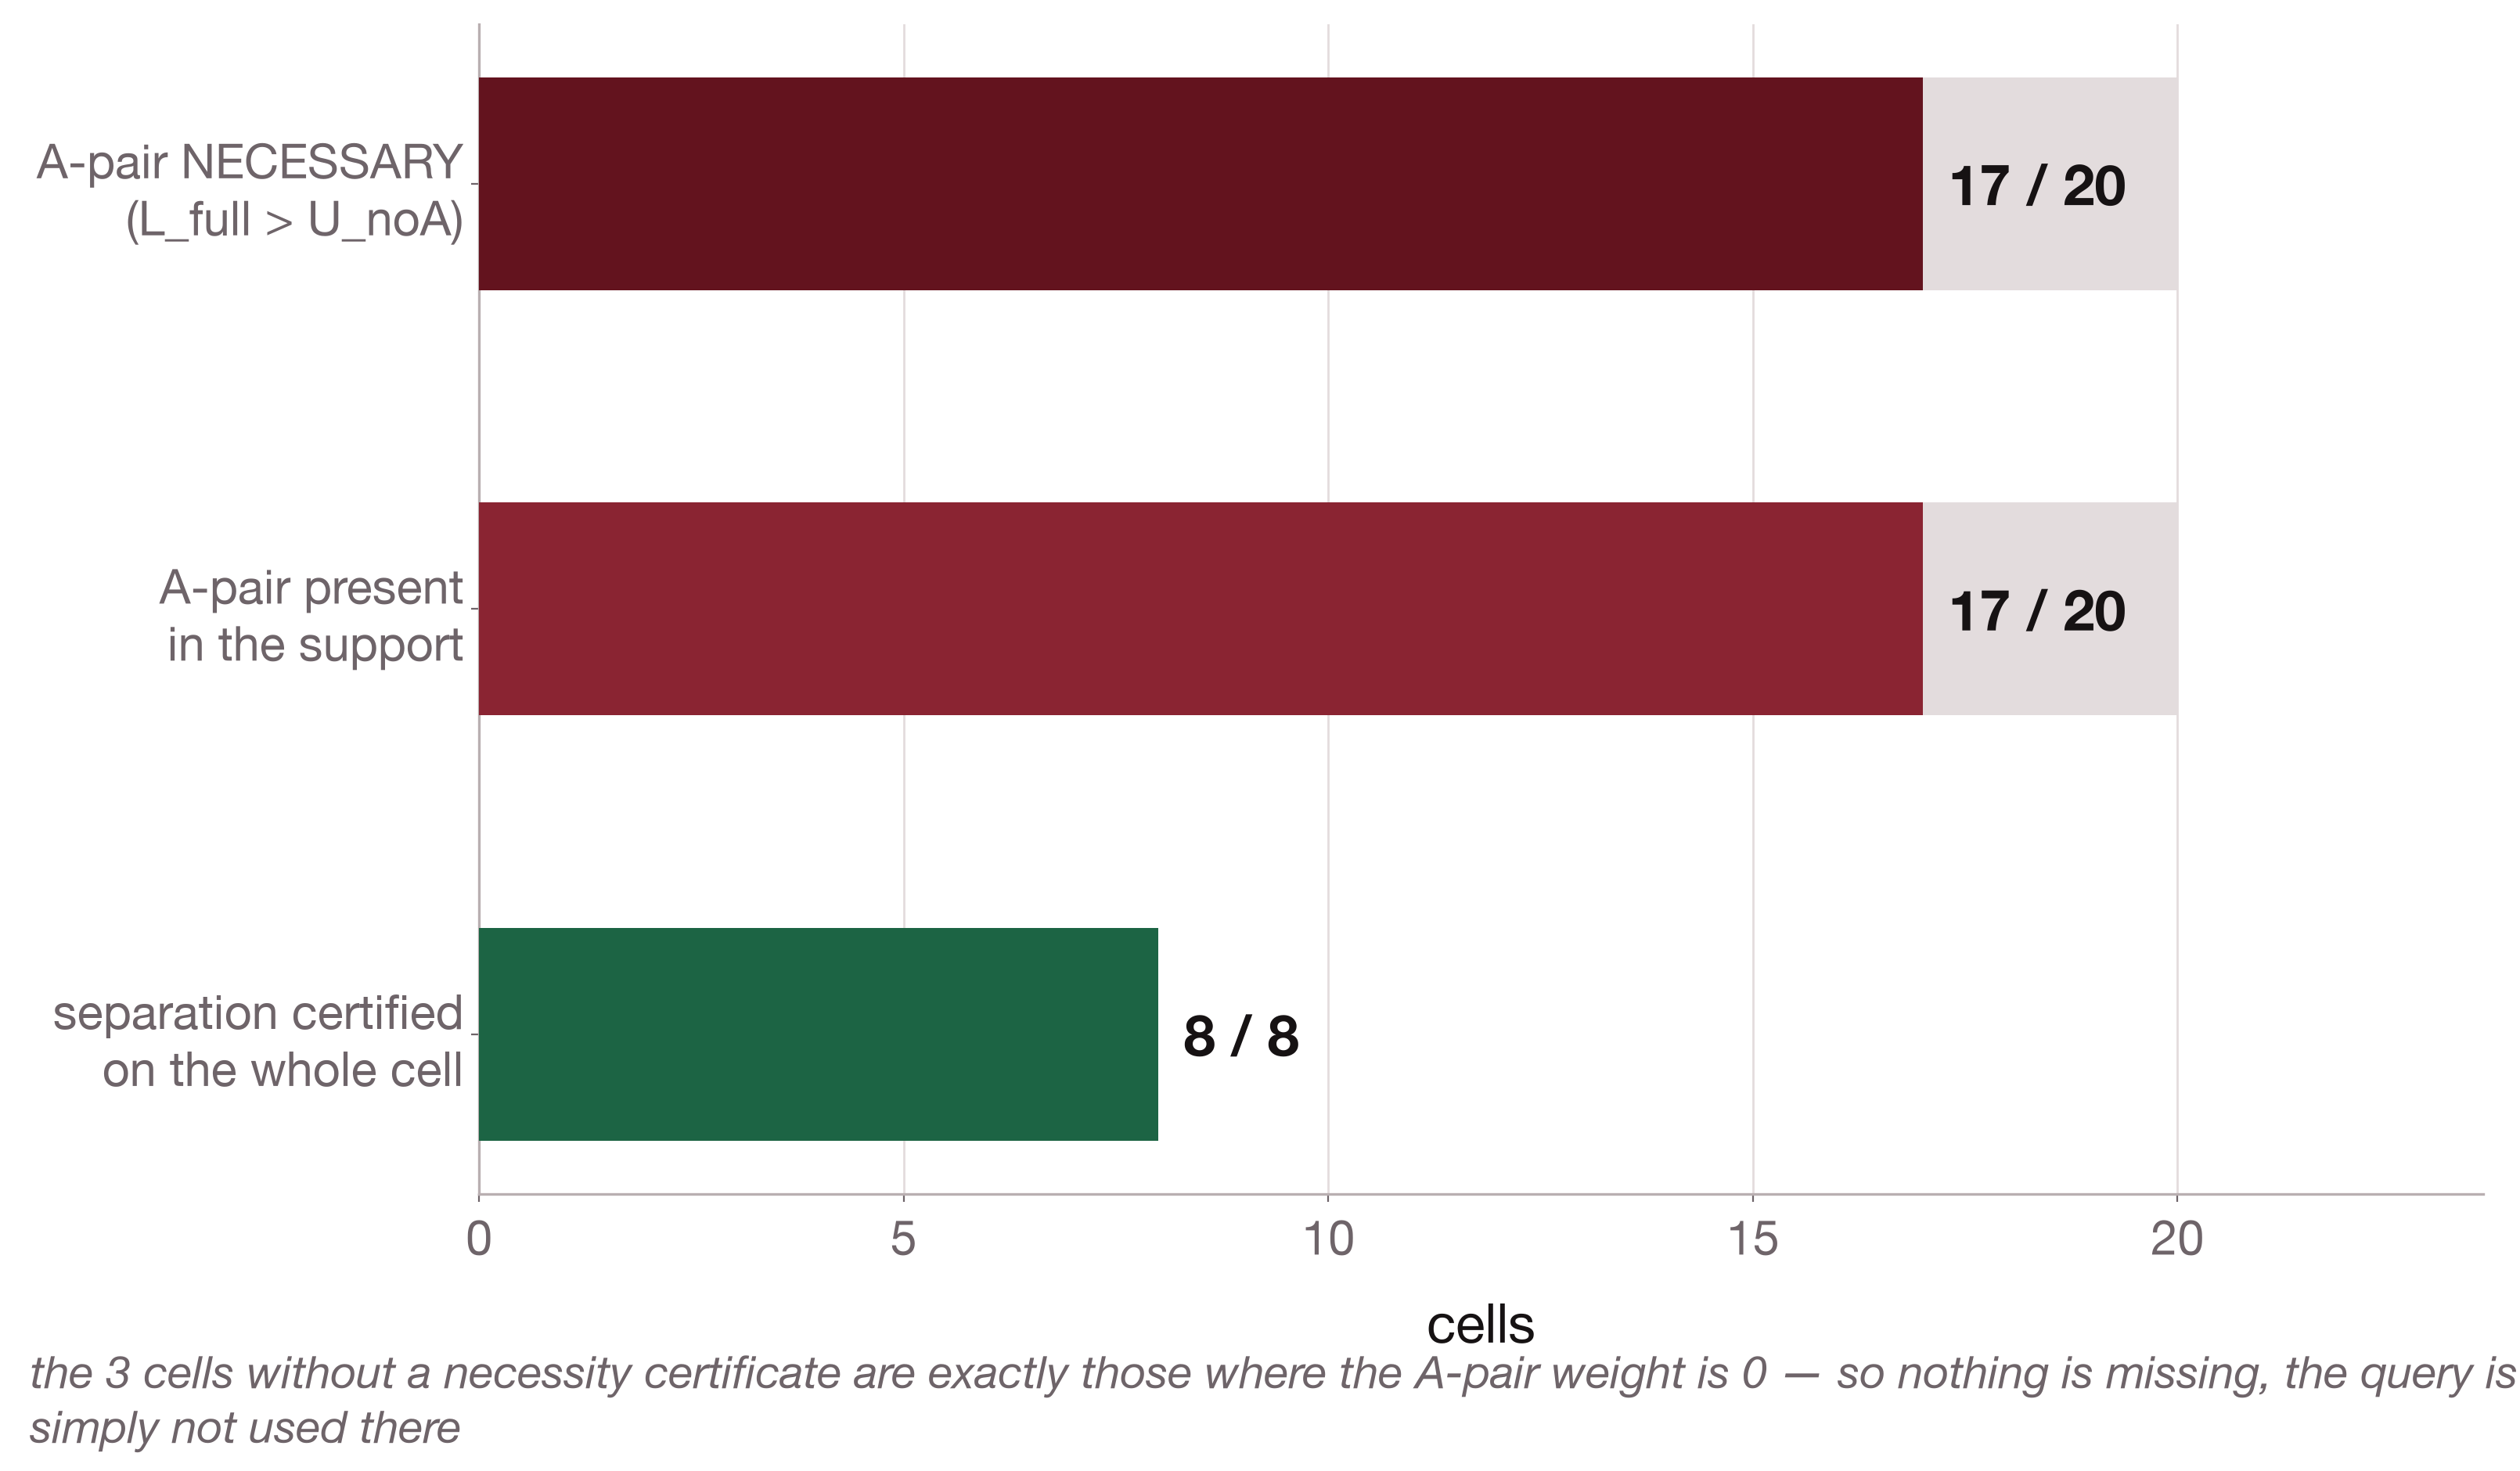
\includegraphics[width=\columnwidth]{d6_fig2_certificates.png}
\caption{Certificate counts. The three cells without a necessity certificate are exactly
those where the pair weight is zero.}
\label{fig:d6-certificates}
\end{figure}

\subsection{How Far From the Corner the Witness Survives}
\label{sec:d6-refsweep}

The sweep of Section~\ref{sec:d6-e2} answers a question the theorems leave open, and the answer
is not the one the first draft of this paper assumed.

At $t=0$ the transcription reproduces both proved statements exactly: the oscillation profile
matches \lean{steered\_span} in all nine validation configurations, and the doubled regret
equals $|A|(2-\rho)$ in all ten corner cells, to the last bit of exact rational arithmetic.
The sweep is therefore measuring the construction the theorems describe.

Away from the corner the construction does not collapse. It degrades, continuously and
predictably. Figure~\ref{fig:d6-reference} plots the doubled regret against $t$: every curve
leaves its corner value $|A|(2-\rho)$ smoothly and decreases monotonically, and no curve
drops discontinuously at any $t>0$. What does happen is that the two failure modes separate.
The hypothesis of Theorem~\ref{thm:d6-subthreshold} fails first in some cells and second in
others. Its hypothesis is that $A$ is a Top-$C$ set; as $t$ grows, the steered coordinate $j$
accumulates oscillation---its span rises from $0$ at the corner to $0.91$ at $t=\tfrac12$ in
the $\rho=1$, $n=6$ cell, while the coordinates of $A$ fall from $1$ to $0.09$---until $j$
overtakes $A$ and the hypothesis is no longer met. Its conclusion is that the regret is
positive, which fails at a different $t$.

The breakdown point of the hypothesis rises with the margin, monotonically and in both
dimensions: at $n=6$ the first flip occurs at $t=\tfrac{7}{32},\tfrac{9}{32},\tfrac{11}{32}$
and $\tfrac{15}{32}$ for $\rho=1,\tfrac54,\tfrac32,\tfrac74$, and at $n=8$ at
$t=\tfrac{5}{32},\tfrac{7}{32},\tfrac{9}{32}$ and $\tfrac38$. Across the sweep $61$ of the
$160$ cells with $t>0$ lose the Top-$C$ property, a rate of $38.1\%$ that falls from $68.8\%$
at $\rho=1$ to $21.9\%$ at $\rho=\tfrac74$. Once a cell flips it stays flipped: the
transition is a single threshold in $t$, not an oscillation. \NUM{}

The $\rho=2$ column is the one to read last. At the threshold margin, $A$ remains a Top-$C$
set at every $t$ on the grid and the doubled regret is non-positive at every $t>0$---the
Top-$C$ set is never beaten. Theorem~\ref{thm:d6-sufficient} is proved for an arbitrary product
reference, so the sweep cannot confirm it in the logical sense; what it does is exercise the
theorem on thirty-two references outside the corner where the necessity construction lives,
and find no violation. Sufficiency and necessity behave differently off the corner in exactly
the direction the proofs predict, which is weak evidence, but it is evidence about the part of
the parameter space no proof here covers.

The practical reading is narrower than the first draft of this paper claimed and broader than
the theorem states. Necessity is proved at $t=0$ and holds, measurably, in a neighbourhood
whose size grows with the margin; it is not a corner-only curiosity, and it is not a theorem
away from the corner either.

\begin{figure}[htbp]
\centering
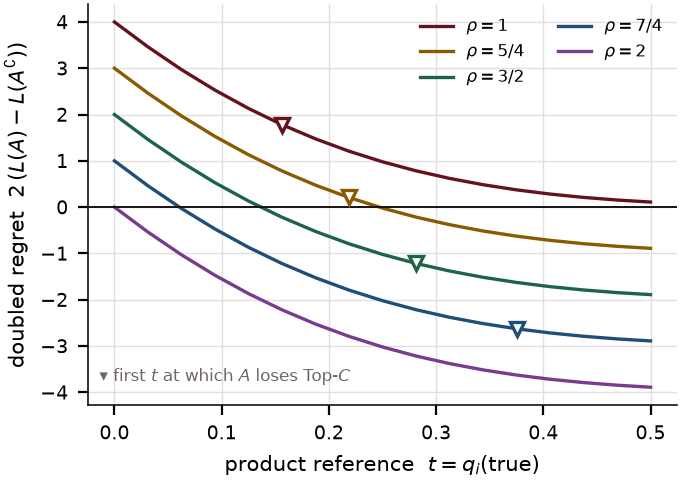
\includegraphics[width=\columnwidth]{d6_fig5_reference.png}
\caption{The necessity construction as the reference leaves the corner, at $n=8$. Each curve
is the doubled regret $2(L(A)-L(A^{\complement}))$ at one margin, in exact rational
arithmetic, against the product reference $q_{i}(\mathrm{true})=t$; at $t=0$ the five curves
begin at $|A|(2-\rho)=4,3,2,1,0$, which is \lean{steered\_exchange\_equality} reproduced by
the transcription rather than assumed by it. Triangles mark the first $t$ at which $A$ ceases
to be a Top-$C$ set, so the hypothesis of Theorem~\ref{thm:d6-subthreshold} stops holding; they
move right as the margin grows and are absent at $\rho=2$, where the set stays Top-$C$
throughout and the regret is non-positive at every $t>0$. The construction degrades with the
reference; it does not fail at the first perturbation. \NUM{}}
\label{fig:d6-reference}
\end{figure}

\subsection{The Finding Is Not an Artefact of the Symmetric Path}
\label{sec:d6-e3results}

Three results from the wider sweep of Section~\ref{sec:d6-e3}, in order of what they rule out.

\emph{The breakdown point is a real function of the margin.} At every one of the three sizes,
the first $t$ at which $A$ ceases to be the Top-$C$ set rises monotonically with the margin,
with no exception and no reversal: at $n=6$ it runs from $13/64$ at $\mu=1$ to $15/32$ at
$\mu=7/4$, at $n=8$ from $5/32$ to $7/16$, and at $n=10$ from $1/8$ to $23/64$.
Figure~\ref{fig:d6-wide} plots all three. The curves also fall with $n$, so the construction
tolerates less perturbation as the space grows---which is worth knowing and which the
single-path sweep could only hint at from two points. The transition is a threshold, not an
oscillation: once a cell flips it stays flipped, at every configuration. \NUM{}

\emph{It is not the symmetric path.} Asymmetric references drawn with an independent $t_{i}$
per coordinate flip the Top-$C$ set at a \emph{higher} rate than the symmetric path,
$49.6\%$ against $42.5\%$, and the four structured directions at a lower one, $19.1\%$. The
symmetric path is therefore neither the most nor the least favourable direction; it sits
inside the range the other directions span, which is what licenses reading it as
representative rather than as special.

\begin{figure}[htbp]
\centering
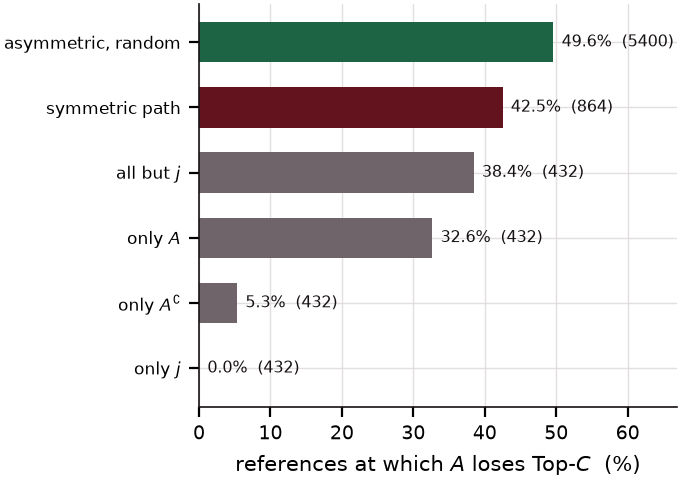
\includegraphics[width=\columnwidth]{d6_fig7_directions.png}
\caption{How often the Top-$C$ set is lost, by the direction the reference is moved in, with
the number of references in each direction in brackets. The symmetric path---the only one the
first sweep used---sits inside the range the other directions span, not at either end:
perturbing only the steered coordinate almost never costs the Top-$C$ property, perturbing
everything but it costs the most among the structured directions, and asymmetric references
drawn independently per coordinate cost more than the symmetric path. Reading the symmetric
path as representative is therefore licensed by measurement rather than by assumption.
\NUM{}}
\label{fig:d6-directions}
\end{figure}

\emph{Sufficiency survives everything tested.} At $\mu=2$, $A$ remains a Top-$C$ set at every
reference in the sweep---$99$ symmetric, $204$ structured and $600$ asymmetric, $903$ in
all---and the doubled regret is non-positive at every one of them.
Theorem~\ref{thm:d6-sufficient} is proved for an arbitrary product reference, so this cannot
confirm it in the logical sense; what it does is exercise the theorem on nine hundred
references outside the corner where the necessity construction lives, including directions
chosen to be awkward, and find no violation. Sufficiency and necessity behave differently off
the corner in exactly the direction the proofs predict. \NUM{}

\begin{figure}[htbp]
\centering
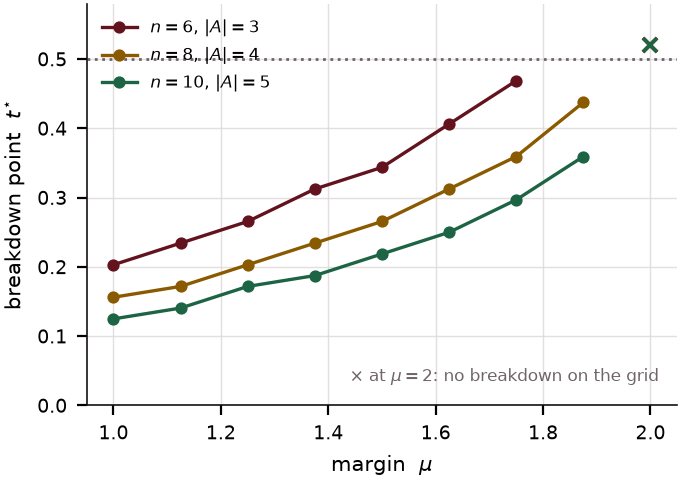
\includegraphics[width=\columnwidth]{d6_fig6_wide.png}
\caption{Where the necessity construction breaks, as a function of the margin, at the three
balanced configurations. Each point is the first $t$ on a sixty-five-point exact grid at
which $A$ stops being a Top-$C$ set, so the hypothesis of
Theorem~\ref{thm:d6-subthreshold} stops holding. The curves rise monotonically with the margin
at every size and fall with the size; the crosses at $\mu=2$ mark that no breakdown occurs
anywhere on the grid there, which is the sufficiency theorem exercised rather than assumed.
Exact rational arithmetic throughout. \NUM{}}
\label{fig:d6-wide}
\end{figure}


\subsection{The Geometry of the Alternative, and What a Scalar Proxy Loses}
\label{sec:fn-results}

\subsection{Reporting Protocol}

All $1{,}000$ paired instances are reported. Median query counts are medians over certified
runs only, and the certification fraction carries the remaining information.

\subsection{The Two Families Separate Without Limit}

As $\eta\to0$ family~1 drives $J_{\mathrm{full}}/J_{\mathrm{scalar}}$ to zero and family~2
drives it to infinity. At $\eta=1$ the two envelopes are $9$ and $0.25$; at $\eta=0.01$ they
are $0.09$ and $6.44$. Both are proved bounds in exact arithmetic, not sampled points, so the
failure of the proxy is a theorem rather than an observation.

\begin{table}[htbp]
\caption{The two families evaluated along the $\eta$ grid. Family~1's column is the proved
upper envelope $9\eta$; family~2's is the proved lower envelope $(1+3\eta)/(16\eta)$. They
move in opposite directions, which is Corollary~\ref{cor:fn-noconstant}.}
\label{tab:fn-families}
\centering
\footnotesize
\begin{tabular}{@{}rrr@{}}
\toprule
$\eta$ & Family 1 ratio $\le$ & Family 2 ratio $\ge$ \\
\midrule
$1.00$ & $9.0000$ & $0.2500$ \\
$0.50$ & $4.5000$ & $0.3125$ \\
$0.20$ & $1.8000$ & $0.5000$ \\
$0.10$ & $0.9000$ & $0.8125$ \\
$0.05$ & $0.4500$ & $1.4375$ \\
$0.02$ & $0.1800$ & $3.3125$ \\
$0.01$ & $0.0900$ & $6.4375$ \\
\bottomrule
\end{tabular}
\end{table}

\subsection{On the Main Panel, $\mathrm{C\_lucb}$ Is the Baseline to Beat}

$\mathrm{C\_lucb}$ certifies $797$ of $1{,}000$ worlds at median $20{,}996$ queries;
$\mathrm{C\_anytime}$ certifies $749$ at $29{,}884$; uniform certifies $605$ at $74{,}252$.
Where both certify---$749$ instances---$\mathrm{C\_lucb}$ is strictly faster in $748$, ties
in $1$ and loses in $0$, with a further $48$ worlds it certifies alone and $0$ that
$\mathrm{C\_anytime}$ certifies alone.

\begin{table}[htbp]
\caption{Confirmatory panel, $1000$ paired instances. A result on this panel under this
generator, not a domination theorem.}
\label{tab:fn-panel}
\centering
\footnotesize
\begin{tabular}{@{}lrrr@{}}
\toprule
Policy & certified & fraction & median $N$ \\
\midrule
$\mathrm{C\_lucb}$    & $797$ & $0.797$ & $20{,}996$ \\
$\mathrm{C\_anytime}$ & $749$ & $0.749$ & $29{,}884$ \\
uniform               & $605$ & $0.605$ & $74{,}252$ \\
\bottomrule
\end{tabular}
\end{table}

\begin{figure}[htbp]
\centering
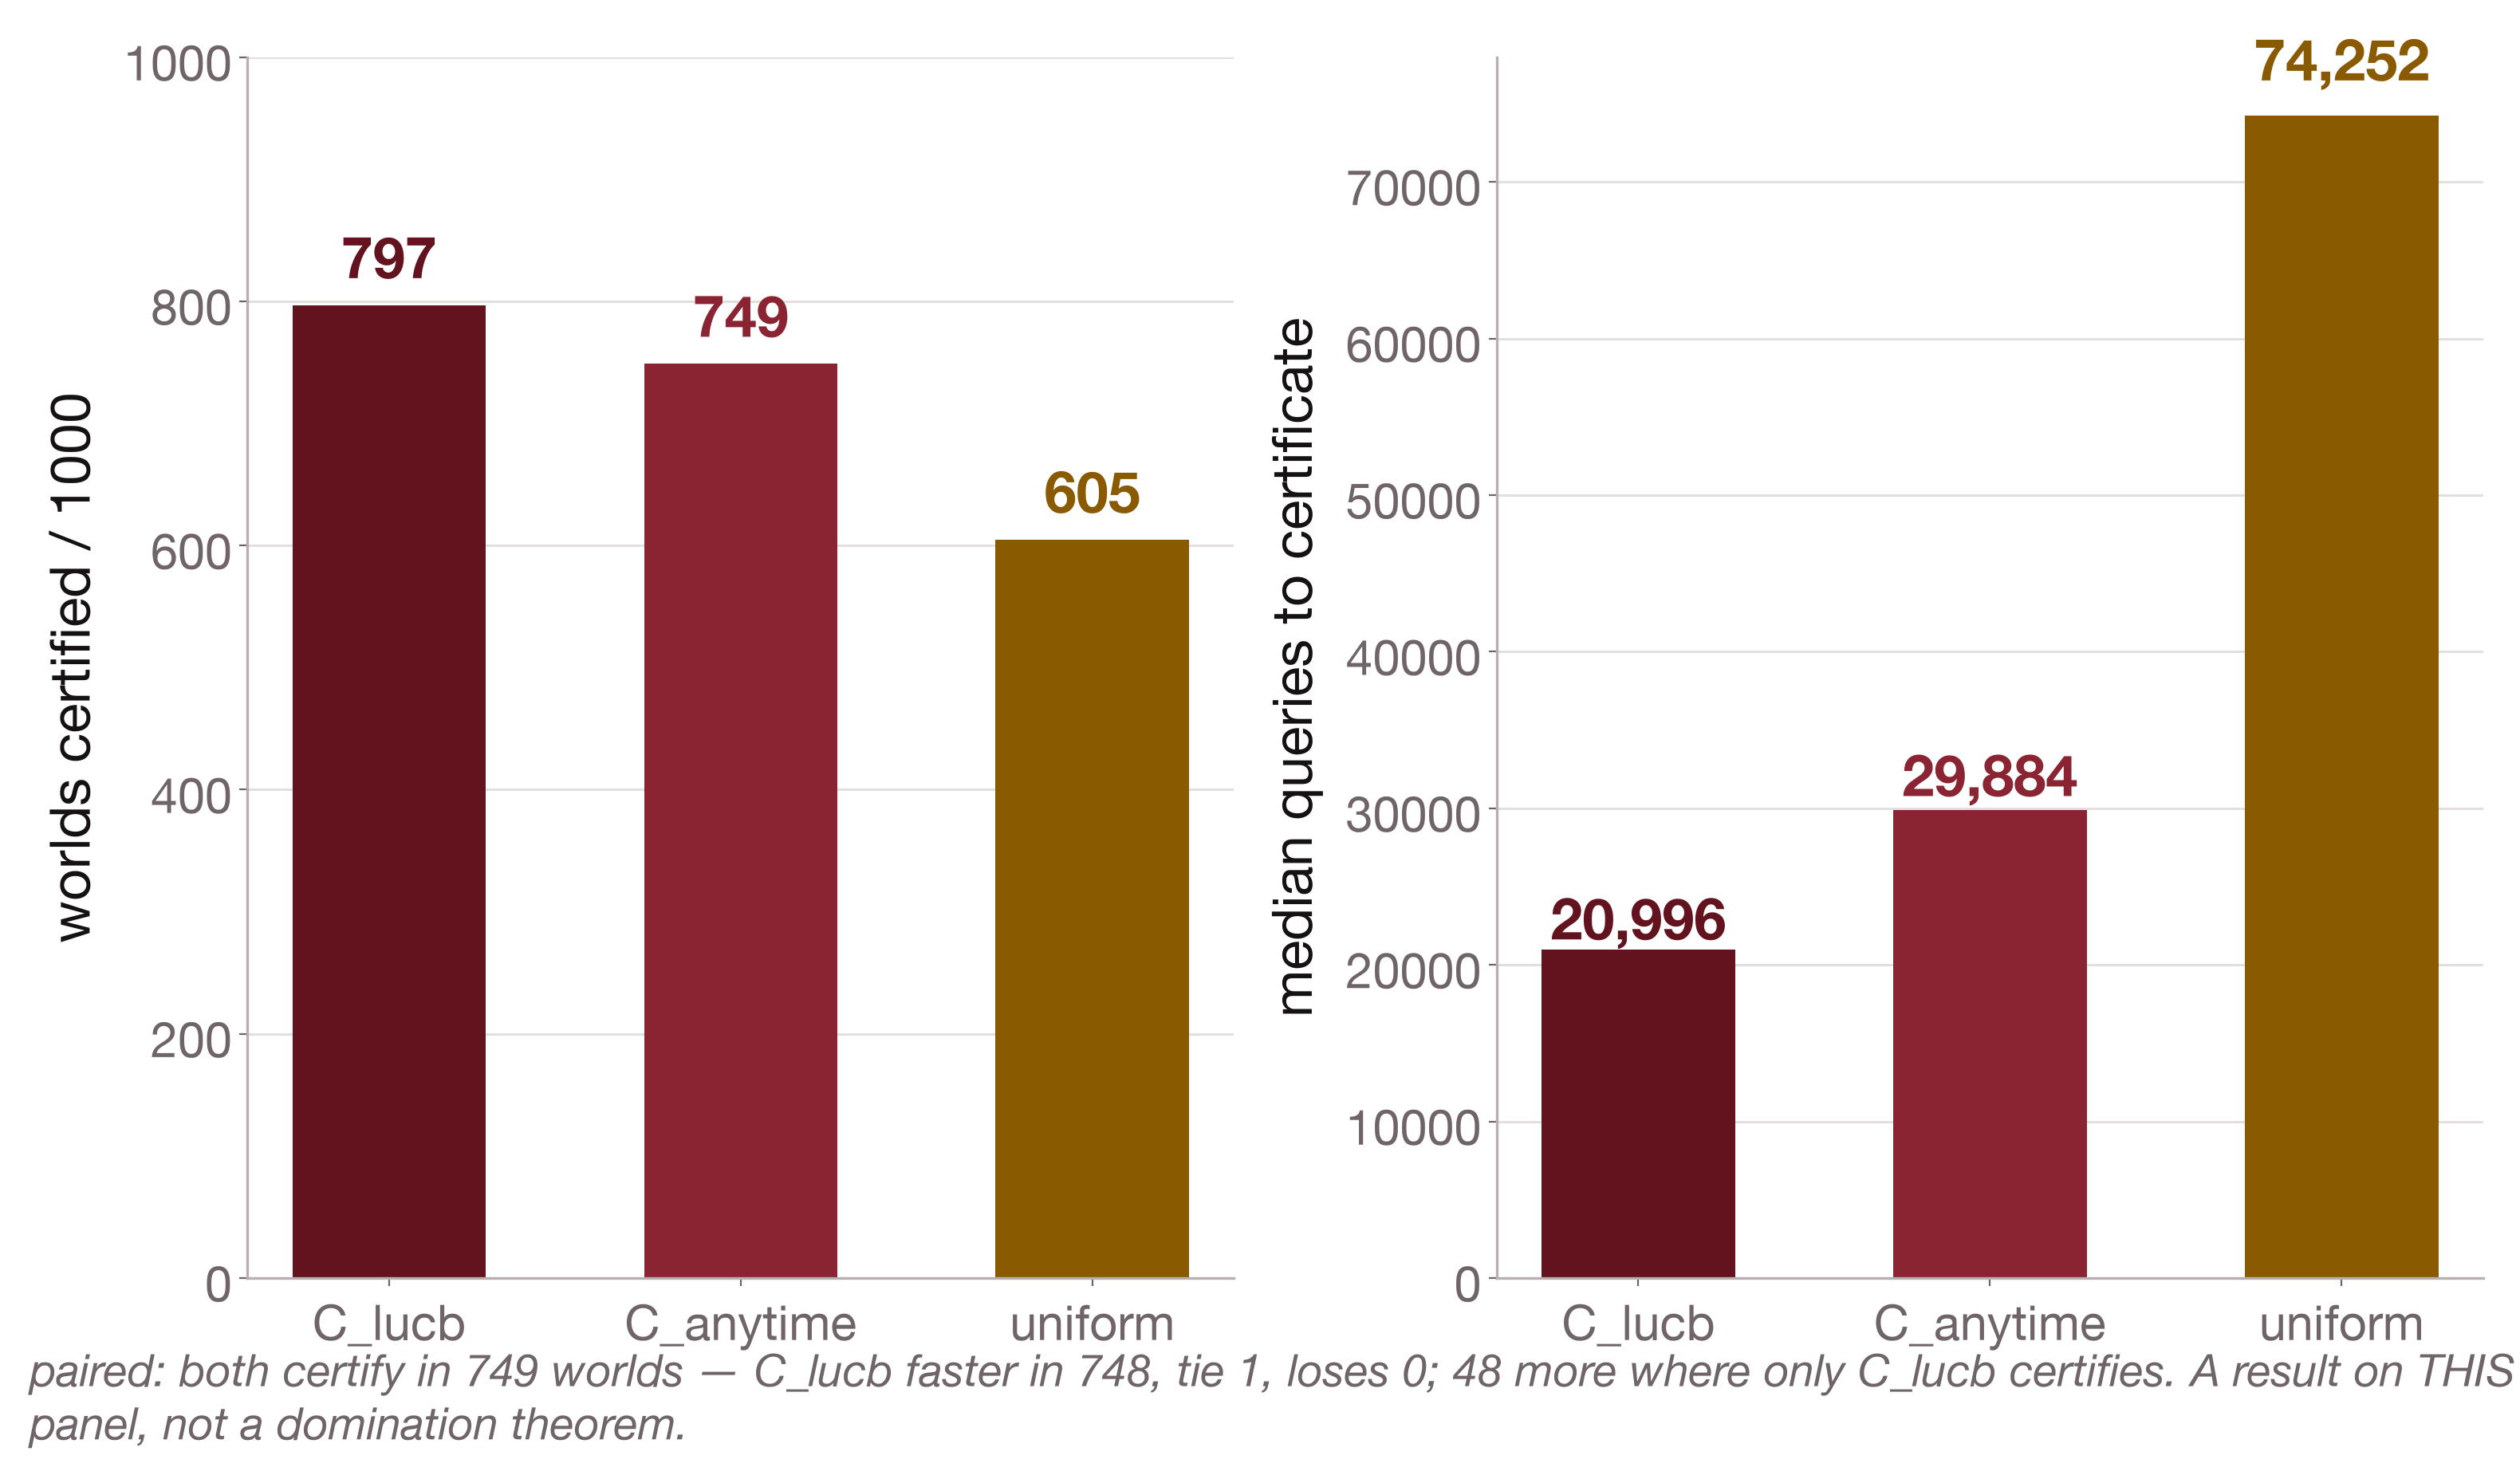
\includegraphics[width=\columnwidth]{func_fig1_panel.png}
\caption{The confirmatory panel, $1000$ paired instances at horizon $131{,}072$.
$\mathrm{C\_lucb}$ is the baseline any new allocator must beat, not a method this paper
defends.}
\label{fig:fn-panel}
\end{figure}

\begin{figure}[htbp]
\centering
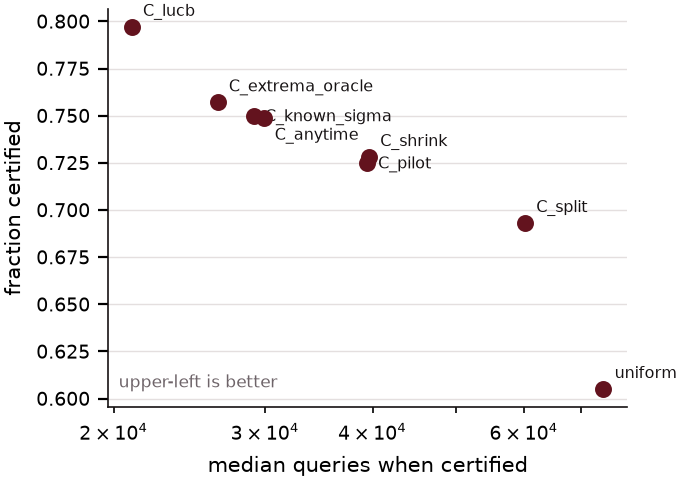
\includegraphics[width=\columnwidth]{func_fig5_panel_detail.png}
\caption{The panel on the two axes that matter jointly. A policy is described by two numbers
at once---how often it certifies, and how many queries it spends when it does---and either
alone can be made to look good at the other's expense. Plotting them together shows that the
ordering here is not a trade-off: $\mathrm{C\_lucb}$ certifies the most worlds \emph{and}
spends the fewest queries doing it, so it dominates on the panel rather than occupying a
different point on a frontier. Uniform allocation sits at the opposite corner on both axes.
This is a panel result under a fixed generator, not a domination theorem. \NUM{}}
\label{fig:fn-paneldetail}
\end{figure}

\subsection{Reading the Panel}

Three things about Table~\ref{tab:fn-panel} should be stated rather than left to inference. It is
a panel result: the generator, horizon and instance distribution are fixed, and the paired
analysis is a property of these instances rather than a proof that $\mathrm{C\_lucb}$ is
never slower. It is not evidence for this paper's oracle, since no allocator built on
Algorithm~\ref{alg:fn-oracle} appears in it. And censoring is substantial at $29.1\%$, which is
why both columns are reported.

\subsection{How Often the Proxy Misleads, and When}
\label{sec:fn-e2results}

Across six thousand instances the scalar proxy is usually close and occasionally far. The
median ratio $J_{\mathrm{full}}/J_{\mathrm{scalar}}$ is $1.000$, so an analyst who uses
\eqref{eq:fn-scalar} on a typical instance is not systematically misled. The tails are another
matter: the fifth percentile is $0.318$ and the ninety-fifth is $1.658$, the extremes reach
$0.018$ and $41.7$, and the proxy is wrong by more than a factor of two on $12.3\%$ of
instances. That figure splits by direction, and the split is the informative part: on
$9.0\%$ the proxy errs optimistically---reporting a value the true problem cannot
deliver---and on the remaining $3.3\%$ it errs conservatively. The two tails are disjoint by
construction, and the optimistic one is nearly three times the size of the other. \NUM{}
\NOTEPAR{An earlier draft reported this as ``wrong by more than a factor of two on
$3.3\%$ \dots and in the optimistic direction on $9.0\%$'', which makes a subset larger than
its superset. The raw rows give $198$ instances above $2\times$ and $542$ below $\tfrac12
\times$, disjoint, $740$ of $6{,}000$ together. The fields are \texttt{frac\_over\_2x} and
\texttt{frac\_under\_half} in \texttt{functional\_proxy.json}.}

The interesting result is not the spread but its cause, and it is the one the families
predict. Figure~\ref{fig:fn-proxy} splits the instances by whether the cheapest
capacity-inverting alternative opens a pair of $j$ other than its current extrema. It does on
$26.6\%$ of instances, and those are a different population: their median ratio is $0.657$
against $1.000$ for the rest. The relationship is not statistical but exact. Of the $1{,}367$
instances on which the proxy overstates---any ratio below one---every single one has a moving
extremum, and so do all $542$ on which it overstates by more than a factor of two. Not one
instance with its extrema fixed produced a ratio below one. The converse fails, as it should:
$1{,}597$ instances have a moving extremum and $230$ of those are still exact, so a moving
extremum is necessary for the proxy to overstate and not sufficient. \NUM{}

That turns the separation from a warning into a test. The mechanism family~1 was built to
exhibit is not a curiosity of a constructed instance---it is what a quarter of random
instances do---and whether it is present can be checked on the instance in hand, before
\eqref{eq:fn-scalar} is trusted, by asking whether the cheapest alternative opens a
currently-extremal pair. Where it does not, the proxy was exact on every instance drawn here.

Two cautions about the computation. First, the exact solver agrees with SLSQP to
$8\times10^{-11}$ on most of the $113$ cross-checked cells, but on a handful the optimiser
comes in far above---up to a factor of six---because the constraint is not smooth and it
stalls. That is a statement about SLSQP, not about the decomposition, and the reason it can
be read that way is the direction: on \emph{no} cell did SLSQP land below the decomposition,
which is the only outcome that would have indicated an error. Second, an earlier
implementation searched only the breakpoints for the optimal window position and therefore
over-estimated $J_{\mathrm{full}}$; it was caught by exactly this cross-check, and the closed
form of Section~\ref{sec:fn-e2} replaced it.

\begin{figure}[htbp]
\centering
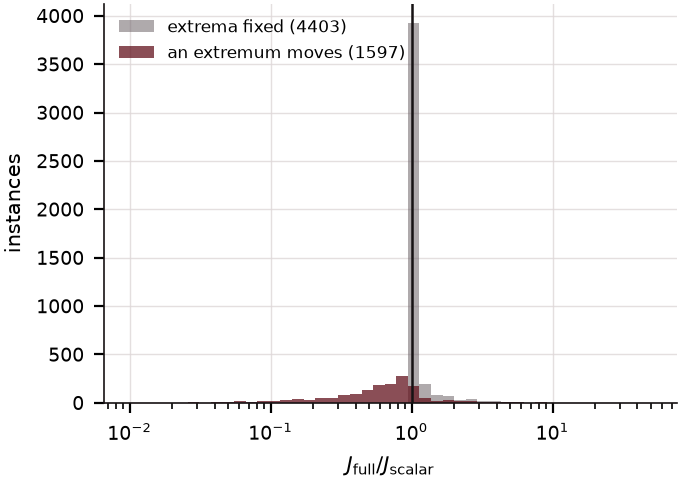
\includegraphics[width=\columnwidth]{func_fig6_proxy.png}
\caption{The scalar proxy against the true value on six thousand random instances, split by
mechanism. The vertical line is exact agreement. Instances where the cheapest alternative
opens a pair that is \emph{not} currently extremal---the mechanism family~1 exploits---carry
almost the whole optimistic tail, with median ratio $0.657$; the rest sit on the line, with
median $1.000$. The proxy's failure is therefore predictable from a property of the instance
rather than being spread uniformly over it. \NUM{}}
\label{fig:fn-proxy}
\end{figure}

\subsection{A Search for a Duality Gap}
\label{sec:fn-e3results}

Theorem~\ref{thm:fn-kkt} is deliberately arranged as sufficiency and deliberately assumes only
semidefiniteness, because an allocator that has learned something loses rank and a certificate
needing $M^{-1}$ fails exactly then. The price of that arrangement is that strong duality is
left open, and it is left open for a reason: the textbook statements are usually quoted under
definiteness or a Slater condition, neither of which is available here.

The question has a sharp refutable form---one instance with a gap settles it---so
Experiment~E3 is run as a search for a counterexample over three families of increasing
awkwardness: $M$ definite, where duality is classical and which therefore serves as the
self-check; $M$ singular; and $M$ singular with its null space deliberately aligned to the
constraint normals, which is the only structural route by which a semidefinite programme can
lose its dual. Over $1{,}054$ solved instances the largest relative gap found is
$1.5\times10^{-11}$ on the definite family, $2.0\times10^{-13}$ on the singular one and
$1.7\times10^{-14}$ on the aligned one---machine precision in every case, and smallest
precisely on the family built to break it. No instance survived re-solution with a gap.
\NUM{}

That is evidence and not a proof, and the asymmetry is worth stating plainly: a single
counterexample would have settled the question, and a thousand instances without one settles
nothing. What the search does establish is narrower and still useful---the mechanism one would
suspect does not produce a gap, so an attempt at the theorem need not work around it.

Two false alarms along the way are worth recording, because both would have been reported as
findings by a less suspicious run. The first was a sign error in the dual objective, caught by
the definite family's self-check, which returned a relative gap of $7\times10^{9}$ rather than
zero. The second was subtler and nearly survived: $\lambda=0$ is always feasible, so the
optimum is frequently zero, and a gap normalised by $|J_{\mathrm{full}}|$ turns a difference of
$10^{-15}$ into an apparent gap of $10^{-2}$. Three instances were flagged that way; the flag
disappeared when the gap was measured against the scale the problem supplies---the objective at
the feasible point $\lambda=0$---rather than against a vanishing optimum. A gap contradicting
classical convex duality is a reason to suspect the measurement first, and here the suspicion
was right twice.

\begin{figure}[htbp]
\centering
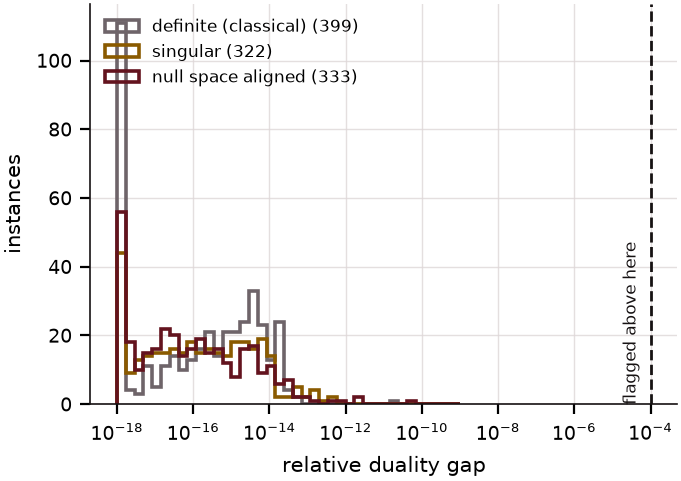
\includegraphics[width=\columnwidth]{func_fig7_duality.png}
\caption{The search for a duality gap on the pair-region programme. Distribution of the
relative gap over three families; the dashed line is the threshold above which an instance is
re-solved from many starts on both sides and re-checked. Nothing reaches it. The family built
to be adversarial---$M$ singular with its null space aligned to the constraint normals---has
the \emph{smallest} gaps of the three, which is the opposite of what a real obstruction would
look like. \NUM{}}
\label{fig:fn-duality}
\end{figure}


\section{Discussion}

\subsection{Certified Compression Under a Known Margin}
\label{sec:d6-discussion}

\subsection{Two Objections of Different Kinds}

The slice objection is about \emph{quantifiers}: it converts a slice-quantified lower bound
into a class-quantified one, and the two-parameter family may now be used without apology.
The provenance objection is about \emph{derivation}: it replaces a fit with an argument, so
the weights are no longer numbers that happened to work in the cells tested. The distinction
matters for how each should be judged, because neither is closed by more data---the $24$ cells
were already consistent, and no quantity of alternatives sampled outside the slice
establishes a universal claim.

Three of the paper's statements sound like limitations and are in fact the contribution.
Corollary~\ref{cor:d6-tight} says the bound cannot be improved by enlarging the class, which
reads as a ceiling but is what makes the reduction free. Theorem~\ref{thm:d6-unique} says there
is no freedom in the weights, which reads as a loss of generality but is what converts a fit
into a derivation. Theorem~\ref{thm:d6-affine} says the optimum is at an endpoint, which reads
as a degenerate answer but is what removes the need to search.

\subsection{Shortcomings and Limitations}
\TODOPAR{Two structural things to settle for the final version. (i) Notation:
$\mu$ denotes both the displacement of the $d$ coordinates in the alternative family
(Sections~I and IV-A) and the margin in the exchange bound (Theorem~\ref{thm:d6-exchange}),
and Theorems~\ref{thm:d6-sufficient}--\ref{thm:d6-subthreshold} then switch to $\rho$ for the same margin while
Section~VII-F switches back. Pick one. (ii) The title carries three propositions and the
margin threshold has nothing to do with the slice or the design; the margin half is a
self-contained result on Top-$C$ selection under approximate modularity and would stand as a
short paper on its own, positioned against Feige--Feldman--Talgam-Cohen on the three axes
Section~II-C already identifies.}

\emph{The reduction is for the scalar query only.} The pair query has a blind direction, so
the coordinate-wise argument of Theorem~\ref{thm:d6-reduction} cannot start: there are non-zero
shifts it cannot see, and no positive lower bound holds uniformly over its class.

\emph{Lower bounds only.} An upper bound quantified over the slice still says nothing about
the class.

\emph{The class is a modelling choice.} An alternative set defined by a norm bound or a
subspace is outside every statement here, and nothing in the formal development can detect a
mismatch, because it is a modelling question. What the development does is make the
hypothesis explicit in the statement.

\emph{The information formulas are premises.} $I_{B}$ and $I_{\mathrm{pair}}$ are taken as
given and not re-derived from the sampling model, so an error in either propagates
downstream---including into \eqref{eq:d6-transitioncond}, which compares them directly.

\emph{The necessity half of the threshold is proved only at the corner.}
Theorem~\ref{thm:d6-subthreshold} is a statement about corner-reference instances and no claim is
proved beyond them. The sweep of Section~\ref{sec:d6-results} shows the situation is better than
that in fact and worse than a theorem: the witness survives a margin-dependent neighbourhood of
the corner and then fails, and $38.1\%$ of the swept positive-$t$ cells lose the Top-$C$
property. Necessity away from the corner is measured, not proved, and this is the most
consequential limitation of the margin results.

\emph{No phase boundary is proved.} Theorem~\ref{thm:d6-affine} identifies where a transition
\emph{can} occur and does not establish that the condition is met anywhere in the parameter
range of interest.

\subsection{Open Problems}

Whether the reduction extends to the pair query, in some form accounting for its blind
direction, is the natural next question. Whether the affine structure survives three or more
query types---where the budget simplex is no longer an interval and an interior optimum
becomes possible---is the second; the objective stays linear so the optimum stays at a
vertex, but the analogue of Proposition~\ref{prop:d6-nonneg} becomes a polytope rather than an
interval and it is not obvious it is cut out as cleanly. Third, whether the sharp threshold
survives a non-corner reference is open: the sweep shows the present construction survives a
margin-dependent neighbourhood of the corner and no further, which locates the question
without settling it.


\subsection{The Geometry of the Alternative, and What a Scalar Proxy Loses}
\label{sec:fn-discussion}

\subsection{What the Families Settle}

The two families settle a methodological question rather than a numerical one. Because the
proxy errs in both directions without a constant, no calibration of it can be safe: an
allocator that trusts it may either waste budget excluding an alternative that is already
cheap (family~1), or stop early against one that is far cheaper than it believes (family~2).
The second is a correctness failure and the first only an efficiency failure, which is why
Corollary~\ref{cor:fn-noconstant} is stated in both directions rather than in the one that is
easier to prove: a one-sided result would leave open that the proxy is conservative, hence
safe if wasteful.

\subsection{Shortcomings and Limitations}
\TODOPAR{The title was narrowed from ``Solving the Group-Range Alternative Exactly'' to
``Exact Components for\dots'' because Section~IV-A says $J_{\mathrm{full}}$ is not formalised
as an infimum and the separability step that assembles the components into an equality is not
proved. \emph{Two ways forward:} prove the separability theorem, which earns the original
title; or keep the current proof and sell the paper as an exact negative result plus exact
components. The second is the shorter path. The abstract's one empirical sentence used to
compare \texttt{C\_lucb} with uniform---neither of them this paper's allocator, as
Section~VII-D says---and now reports the E2 measurement instead.}

\emph{The decomposition step is not formalised, so the oracle equality is not claimed.} The
chain of Sections~\ref{sec:fn-union}--\ref{sec:fn-kkt} would become an equality
$J_{\mu}(x)=\min_{i,j}\inf_{z\ge0}[S_{i}(z)+E_{j}(z)]$ given one further statement: that in
the observation model the two relations occupy disjoint blocks of the information matrix
while every other relation contributes zero cost. That is a \emph{model} statement, not an
optimisation one, and it is not proved here. Each component of the chain is proved, and the
inequalities \eqref{eq:fn-order} are proved; what is missing is precisely the separability step.
Stating this plainly costs the paper a headline, and the alternative---presenting the chain as
though it closed---would forfeit the discipline the rest of the paper rests on. The negative
results do not depend on the assembly: they compare $J_{\mathrm{full}}$ against
$J_{\mathrm{scalar}}$ directly, bounded above by an exhibited alternative in family~1 and
below by Lemma~\ref{lem:fn-posparts} in family~2.

\emph{The certificate is sufficiency only.} Theorem~\ref{thm:fn-kkt} says a point with a
certificate is optimal. It does not say every optimal point has one, and only weak duality is
proved, so a duality gap is not excluded.

\emph{Standing model assumptions.} Free response table, known variance, positive precision.
Under realizability coupling the cost does not separate and nothing here applies.

\emph{No allocator has been built.} Table~\ref{tab:fn-panel} is a statement about existing
policies and not evidence for the oracle. The paper establishes that the exact oracle is
computable and that the proxy is unusable; it does not establish that the exact oracle pays
for itself.

\emph{The families are extremal by construction.} What happens on ordinary instances is not
measured, and deliberately so: the error depends on how far the cheapest alternative's
attaining cells are from the truth's, which is an instance property with no natural
distribution attached, so a sweep would report a property of the generator.

\subsection{Open Problems}

Assembling the full oracle equality is first, and it requires the separability statement named
above rather than more optimisation. Building an allocator on the exact oracle and comparing
it against $\mathrm{C\_lucb}$ on the same panel is second. Whether strong duality holds for
the pair-region programme is third; Section~\ref{sec:fn-e3results} searched $1{,}054$ instances
for a gap, including a family built to produce one, and found none above machine precision,
which locates the question without answering it. Finally, the families are two-relation and three-action;
whether the failure ratios can be driven to their limits with fewer actions, or must worsen
with more relations, is not known.


\section{Conclusion}

\subsection{Certified Compression Under a Known Margin}

The two-parameter alternative family is not a restriction: every alternative in its class
costs at least the slice value, and the bound is attained on the slice. The design
that reproduces the corpus's coefficients is not fitted: it is forced by the budget constraint
and the split, depends only on the split and the price, and makes the delivered information
affine, so the optimal design is pure except on an explicitly computable threshold. And the
margin at which Top-$C$ selection stops being optimal is sharp at $2\delta$: sufficient under
every product reference, and violated below it by an explicit construction under the corner
reference. The wider point concerns how a corpus of results should be maintained. Both
objections answered here were raised against statements that were, numerically, entirely
correct; what was missing in each case was an argument connecting the statement to the claim
it was used to support, and in both cases that argument turned out to be short.



\subsection{The Geometry of the Alternative, and What a Scalar Proxy Loses}

When the extrema can move, the scalar pair-flip proxy is a bound in neither direction, and no
constant repairs it. The true alternative set is a finite union of convex pair regions on the
real range target; its energy oracle is a finite conjunction of convex problems; the inner
problem has a closed form; and its optimality certificate needs no matrix inverse, so a
singular information matrix costs nothing extra. For a practitioner the guidance is concrete.
If relations are ranked by a mean, the pair-flip value is exact and nothing here applies. If
they are ranked by a range, or by any statistic whose attaining cells can move, do not compute
the value at the current extrema: enumerate the ordered pairs, evaluate the shrink and expand
costs on each, and take the minimum.



\section*{Acknowledgment}

\begin{thebibliography}{00}

\bibitem{pukelsheim2006} F. Pukelsheim, \emph{Optimal Design of Experiments}. Philadelphia,
PA: SIAM Classics in Applied Mathematics, 2006.

\bibitem{fedorov1972} V. V. Fedorov, \emph{Theory of Optimal Experiments}. New York, NY:
Academic Press, 1972.

\bibitem{boyd2004} S. Boyd and L. Vandenberghe, \emph{Convex Optimization}. Cambridge,
U.K.: Cambridge Univ. Press, 2004.

\bibitem{feige2020} U. Feige, M. Feldman, and I. Talgam-Cohen, ``Approximate modularity
revisited,'' \emph{SIAM J. Comput.}, vol.~49, no.~1, pp.~67--97, 2020.

\bibitem{moore2009} R. E. Moore, R. B. Kearfott, and M. J. Cloud, \emph{Introduction to
Interval Analysis}. Philadelphia, PA: SIAM, 2009.

\bibitem{mathlib2020} The mathlib Community, ``The Lean mathematical library,'' in
\emph{Proc. 9th ACM SIGPLAN Int. Conf. Certified Programs and Proofs (CPP)}, 2020,
pp.~367--381.

\bibitem{demoura2021} L. de Moura and S. Ullrich, ``The Lean 4 theorem prover and
programming language,'' in \emph{Proc. 28th Int. Conf. Automated Deduction (CADE)}, 2021,
pp.~625--635.

\bibitem{garivier2016} A. Garivier and E. Kaufmann, ``Optimal best arm identification with
fixed confidence,'' in \emph{Proc. 29th Annu. Conf. Learning Theory (COLT)}, 2016.

\bibitem{kaufmann2016} E. Kaufmann, O. Capp\'e, and A. Garivier, ``On the complexity of
best-arm identification in multi-armed bandit models,'' \emph{J. Mach. Learn. Res.},
vol.~17, pp.~1--42, 2016.

\bibitem{jourdan2023} M. Jourdan, R. Degenne, and E. Kaufmann, ``Dealing with unknown
variances in best-arm identification,'' in \emph{Proc. 34th Int. Conf. Algorithmic Learning
Theory (ALT)}, 2023.

\bibitem{rockafellar1970} R. T. Rockafellar, \emph{Convex Analysis}. Princeton, NJ:
Princeton Univ. Press, 1970.

\end{thebibliography}

\appendices
\section{Complete statement inventory}
\label{app:d6-inventory}

The D6 strand contributes $187$ axiom-audited theorems and lemmas across its accepted modules. Those that any step of this paper uses are displayed in Section~\ref{sec:d6-setting}, beside the step that consumes them. This appendix reproduces the \emph{complete} chain---every audited statement of the strand, grouped by module, including the ones already shown---so that the development can be read end to end without reassembling it from the body.

Each entry is a symbol-level transliteration of the Lean statement: Unicode maps to the corresponding \LaTeX{} symbol and identifiers are set upright, but no structure is rewritten and no hypothesis is dropped. Binders are listed as the prover has them and the turnstile $\vdash$ separates them from the conclusion. Every entry carries an acceptance receipt and an axiom audit confining it to $\{\textsf{propext},\textsf{Classical.choice},\textsf{Quot.sound}\}$; none contains \texttt{sorry}.

\vspace{4pt}\noindent\rule{\columnwidth}{0.4pt}\par\vspace{2pt}
\noindent\textbf{Module \lean{LeanD6AlternativeReductionV1}}\par\vspace{3pt}

\noindent\textbf{A\,1}\quad\lean{crossing\_bracket}
{\footnotesize\[ \begin{aligned}[t]
&(\mathit{f} : \mathbb{R} \to \mathbb{R} ),\; (\mathit{t0} \mathit{t1} : \mathbb{R} ),\; (\mathit{ht} : \mathit{t0} \leq \mathit{t1}),\; (\mathit{hc} :\\
&\quad \mathit{ContinuousOn} \mathit{f} (\mathit{Set}.\mathit{Icc} \mathit{t0} \mathit{t1})),\; (\mathit{h0} : \mathit{f} \mathit{t0} \leq 0),\; (\mathit{h1} : 0 \leq \mathit{f} \mathit{t1})\\
\vdash\;&\exists \mathit{t} \in \mathit{Set}.\mathit{Icc} \mathit{t0} \mathit{t1}, \mathit{f} \mathit{t} = 0
\end{aligned} \]}

\noindent\textbf{A\,2}\quad\lean{no\_crossing\_of\_modulus}
{\footnotesize\[ \begin{aligned}[t]
&(\mathit{f} : \mathbb{R} \to \mathbb{R} ),\; (\mathit{t0} \mathit{t1} \mathit{Lip} \mathit{m} : \mathbb{R} ),\; (\mathit{ht} : \mathit{t0} \leq \mathit{t1}),\\
&\quad \; (\mathit{hLip} : 0 \leq \mathit{Lip}),\; (\mathit{hlip} : \forall \mathit{s} \in \mathit{Set}.\mathit{Icc} \mathit{t0} \mathit{t1}, |\mathit{f} \mathit{s} - \mathit{f} \mathit{t0}| \leq\\
&\quad \mathit{Lip} * (\mathit{s} - \mathit{t0})),\; (\mathit{hm} : \mathit{m} \leq \mathit{f} \mathit{t0}),\; (\mathit{hpos} : 0 < \mathit{m}),\\
&\quad \; (\mathit{hgap} : \mathit{Lip} * (\mathit{t1} - \mathit{t0}) < \mathit{m})\\
\vdash\;&\forall \mathit{t} \in \mathit{Set}.\mathit{Icc} \mathit{t0} \mathit{t1}, 0 < \mathit{f} \mathit{t}
\end{aligned} \]}

\noindent\textbf{A\,3}\quad\lean{quadratic\_ge\_vertex}
{\footnotesize\[ \begin{aligned}[t]
&(\mathit{a} \mathit{b} \mathit{c} \mathit{x} : \mathbb{R} ),\; (\mathit{ha} : 0 < \mathit{a})\\
\vdash\;&\mathit{a} * (-\mathit{b} / (2 * \mathit{a})) ^{2} + \mathit{b} * (-\mathit{b} / (2 * \mathit{a})) + \mathit{c} \leq\\
&\quad \mathit{a} * \mathit{x} ^{2} + \mathit{b} * \mathit{x} + \mathit{c}
\end{aligned} \]}

\noindent\textbf{A\,4}\quad\lean{quadratic\_inf\_Icc}
{\footnotesize\[ \begin{aligned}[t]
&(\mathit{a} \mathit{b} \mathit{c} \mathit{lo} \mathit{hi} \mathit{x} : \mathbb{R} ),\; (\mathit{ha} : 0 < \mathit{a}),\; (\mathit{hx1} : \mathit{lo} \leq \mathit{x}),\; (\mathit{hx2} : \mathit{x} \leq \mathit{hi})\\
\vdash\;&\mathit{min} (\mathit{min} (\mathit{a} * \mathit{lo} ^{2} + \mathit{b} * \mathit{lo} + \mathit{c}) (\mathit{a} * \mathit{hi} ^{2} + \mathit{b} * \mathit{hi} + \mathit{c})) (\mathit{a} * (-\\
&\quad \mathit{b} / (2 * \mathit{a})) ^{2} + \mathit{b} * (-\mathit{b} / (2 * \mathit{a})) + \mathit{c}) \leq \mathit{a} * \mathit{x} ^{2} + \mathit{b} * \mathit{x} + \mathit{c}
\end{aligned} \]}

\noindent\textbf{A\,5}\quad\lean{quadratic\_inf\_attained}
{\footnotesize\[ \begin{aligned}[t]
&(\mathit{a} \mathit{b} \mathit{c} \mathit{lo} \mathit{hi} : \mathbb{R} ),\; (\mathit{ha} : 0 < \mathit{a}),\; (\mathit{hv1} : \mathit{lo} \leq -\mathit{b} / (2 * \mathit{a})),\\
&\quad \; (\mathit{hv2} : -\mathit{b} / (2 * \mathit{a}) \leq \mathit{hi})\\
\vdash\;&(\forall \mathit{x}, \mathit{lo} \leq \mathit{x} \to \mathit{x} \leq \mathit{hi} \to \mathit{a} * (-\mathit{b} / (2 * \mathit{a})) ^{2} + \mathit{b} * (-\mathit{b} / (\\
&\quad 2 * \mathit{a})) + \mathit{c} \leq \mathit{a} * \mathit{x} ^{2} + \mathit{b} * \mathit{x} + \mathit{c}) \wedge \mathit{lo} \leq -\mathit{b} / (2 * \mathit{a}) \wedge\\
&\quad -\mathit{b} / (2 * \mathit{a}) \leq \mathit{hi}
\end{aligned} \]}

\noindent\textbf{A\,6}\quad\lean{quadratic\_inf\_endpoint\_left}
{\footnotesize\[ \begin{aligned}[t]
&(\mathit{a} \mathit{b} \mathit{c} \mathit{lo} \mathit{hi} \mathit{x} : \mathbb{R} ),\; (\mathit{ha} : 0 < \mathit{a}),\; (\mathit{hv} : -\mathit{b} / (2 * \mathit{a}) \leq \mathit{lo}),\\
&\quad \; (\mathit{hx1} : \mathit{lo} \leq \mathit{x}),\; (\mathit{hx2} : \mathit{x} \leq \mathit{hi})\\
\vdash\;&\mathit{a} * \mathit{lo} ^{2} + \mathit{b} * \mathit{lo} + \mathit{c} \leq \mathit{a} * \mathit{x} ^{2} + \mathit{b} * \mathit{x} + \mathit{c}
\end{aligned} \]}

\noindent\textbf{A\,7}\quad\lean{quadratic\_inf\_endpoint\_right}
{\footnotesize\[ \begin{aligned}[t]
&(\mathit{a} \mathit{b} \mathit{c} \mathit{lo} \mathit{hi} \mathit{x} : \mathbb{R} ),\; (\mathit{ha} : 0 < \mathit{a}),\; (\mathit{hv} : \mathit{hi} \leq -\mathit{b} / (2 * \mathit{a})),\\
&\quad \; (\mathit{hx1} : \mathit{lo} \leq \mathit{x}),\; (\mathit{hx2} : \mathit{x} \leq \mathit{hi})\\
\vdash\;&\mathit{a} * \mathit{hi} ^{2} + \mathit{b} * \mathit{hi} + \mathit{c} \leq \mathit{a} * \mathit{x} ^{2} + \mathit{b} * \mathit{x} + \mathit{c}
\end{aligned} \]}

\vspace{4pt}\noindent\rule{\columnwidth}{0.4pt}\par\vspace{2pt}
\noindent\textbf{Module \lean{LeanD6ApproximateActualEvaluatorV1}}\par\vspace{3pt}

\noindent\textbf{A\,8}\quad\lean{actual\_label\_infimum}
{\footnotesize\[ \begin{aligned}[t]
&(\mathit{A} \mathit{B} \mathit{C} : \mathit{Finset} (\mathit{I} \mathit{n})),\; (\mathit{j} : \mathit{I} \mathit{n}),\; (\mathit{hjC} : \mathit{j} \notin \mathit{C}),\; (\mathit{q} \mathit{mu} \mathit{eps} : \mathbb{R} ),\\
&\quad \; (\mathit{he} : 0 \leq \mathit{eps}),\; (\mathit{hd} : \mathit{eps} < (\mathit{exchange} \mathit{C} \mathit{B} : \mathbb{R} )),\\
&\quad \; (\mathit{E} : \mathit{Finset} (\mathit{Measurement} \mathit{n})),\; (\mathit{w} : \mathit{Measurement} \mathit{n} \to \mathbb{R} ),\\
&\quad \; (\mathit{hl} : \forall \mathit{e} \in \mathit{E},\mathit{Legal} \mathit{j} \mathit{q} \mathit{e}),\; (\mathit{hw} : \forall \mathit{e} \in \mathit{E},0 \leq \mathit{w} \mathit{e})\\
\vdash\;&\mathit{sInf} (\mathit{labelCosts} \mathit{A} \mathit{B} \mathit{C} \mathit{j} \mathit{mu} \mathit{eps} \mathit{E} \mathit{w})=\mathit{evaluator} \mathit{A} \mathit{B} \mathit{C} \mathit{j} \mathit{mu} \mathit{eps} \mathit{E} \mathit{w}
\end{aligned} \]}

\noindent\textbf{A\,9}\quad\lean{curvature\_nonneg}
{\footnotesize\[ \begin{aligned}[t]
&(\mathit{B} : \mathit{Finset} (\mathit{I} \mathit{n})),\; (\mathit{j} : \mathit{I} \mathit{n}),\; (\mathit{E} : \mathit{Finset} (\mathit{Measurement} \mathit{n})),\\
&\quad \; (\mathit{w} : \mathit{Measurement} \mathit{n} \to \mathbb{R} ),\; (\mathit{hw} : \forall \mathit{e} \in \mathit{E},0 \leq \mathit{w} \mathit{e})\\
\vdash\;&0 \leq \mathit{curvature} \mathit{B} \mathit{j} \mathit{E} \mathit{w}
\end{aligned} \]}

\noindent\textbf{A\,10}\quad\lean{zero\_curvature\_cross}
{\footnotesize\[ \begin{aligned}[t]
&(\mathit{A} \mathit{B} : \mathit{Finset} (\mathit{I} \mathit{n})),\; (\mathit{j} : \mathit{I} \mathit{n}),\; (\mathit{mu} : \mathbb{R} ),\; (\mathit{E} : \mathit{Finset} (\\
&\quad \mathit{Measurement} \mathit{n})),\; (\mathit{w} : \mathit{Measurement} \mathit{n} \to \mathbb{R} ),\; (\mathit{hw} : \forall \mathit{e} \in \mathit{E},\\
&\quad 0 \leq \mathit{w} \mathit{e}),\; (\mathit{hc} : \mathit{curvature} \mathit{B} \mathit{j} \mathit{E} \mathit{w}=0)\\
\vdash\;&\mathit{crossTerm} \mathit{A} \mathit{B} \mathit{j} \mathit{mu} \mathit{E} \mathit{w}=0
\end{aligned} \]}

\vspace{4pt}\noindent\rule{\columnwidth}{0.4pt}\par\vspace{2pt}
\noindent\textbf{Module \lean{LeanD6CalibrationActiveFaceV1}}\par\vspace{3pt}

\noindent\textbf{A\,11}\quad\lean{active\_iff\_cross\_zero}
{\footnotesize\[ \begin{aligned}[t]
&(\mathit{D} \mathit{M} : \mathit{Alt} \to \mathbb{R} ),\; (\mathit{Gamma} : \mathbb{R} ),\; (\mathit{a} : \mathit{Alt}),\; (\mathit{hactive} : \mathit{D} \mathit{a} =\\
&\quad \mathit{Gamma})\\
\vdash\;&\mathit{Gamma} \leq \mathit{profiled} \mathit{D} \mathit{M} \mathit{a} \leftrightarrow \mathit{M} \mathit{a} = 0
\end{aligned} \]}

\noindent\textbf{A\,12}\quad\lean{active\_nonzero\_forces\_loss}
{\footnotesize\[ \begin{aligned}[t]
&(\mathit{D} \mathit{M} : \mathit{Alt} \to \mathbb{R} ),\; (\mathit{Gamma} : \mathbb{R} ),\; (\mathit{a} : \mathit{Alt}),\; (\mathit{hactive} : \mathit{D} \mathit{a} =\\
&\quad \mathit{Gamma}),\; (\mathit{hcross} : \mathit{M} \mathit{a} \neq 0)\\
\vdash\;&\mathit{profiled} \mathit{D} \mathit{M} \mathit{a} < \mathit{Gamma}
\end{aligned} \]}

\noindent\textbf{A\,13}\quad\lean{profile\_formula\_unit}
{\footnotesize\[ \begin{aligned}[t]
&\{ \mathit{E} : \mathit{Type}*\},\; [\mathit{Fintype} \mathit{E}],\; (\mathit{w} \mathit{d} : \mathit{E} \to \mathbb{R} ),\; (\mathit{hcurv} : \mathit{curvature} \mathit{w} (\\
&\quad \mathbf{fun} \mathit{\_} => 1) = 1)\\
\vdash\;&\mathit{energy} \mathit{w} \mathit{d} (\mathbf{fun} \mathit{\_} => 1) (\mathit{cross} \mathit{w} \mathit{d} (\mathbf{fun} \mathit{\_} => 1)) =\\
&\quad \mathit{raw} \mathit{w} \mathit{d} / 2 - (\mathit{cross} \mathit{w} \mathit{d} (\mathbf{fun} \mathit{\_} => 1))^{2} / 2
\end{aligned} \]}

\noindent\textbf{A\,14}\quad\lean{profiled\_ge\_iff}
{\footnotesize\[ \begin{aligned}[t]
&(\mathit{D} \mathit{M} : \mathit{Alt} \to \mathbb{R} ),\; (\mathit{Gamma} : \mathbb{R} ),\; (\mathit{hknown} : \forall \mathit{a}, \mathit{Gamma} \leq \mathit{D} \mathit{a})\\
\vdash\;&(\forall \mathit{a}, \mathit{Gamma} \leq \mathit{profiled} \mathit{D} \mathit{M} \mathit{a}) \leftrightarrow \forall \mathit{a}, (\mathit{M} \mathit{a})^{2} \leq 2 * \mathit{slack} \mathit{D} \mathit{Gamma}\\
&\quad \mathit{a}
\end{aligned} \]}

\vspace{4pt}\noindent\rule{\columnwidth}{0.4pt}\par\vspace{2pt}
\noindent\textbf{Module \lean{LeanD6CenterAnswerGeometryV1}}\par\vspace{3pt}

\noindent\textbf{A\,15}\quad\lean{boundary\_arbitrarily\_small}
{\footnotesize\[ \begin{aligned}[t]
&(\mathit{A} \mathit{B} : \mathit{Finset} (\mathit{I} \mathit{n})),\; (\mathit{j} : \mathit{I} \mathit{n}),\; (\mathit{hj} : \mathit{j} \notin \mathit{A}),\; (\mathit{q} \mathit{mu} : \mathbb{R} ),\\
&\quad \; (\mathit{hmu0} : 0 < \mathit{mu}),\; (\mathit{hmu1} : \mathit{mu} \leq 1),\; (\mathit{E} : \mathit{Finset} (\\
&\quad \mathit{Measurement} \mathit{n})),\; (\mathit{w} : \mathit{Measurement} \mathit{n} \to \mathbb{R} ),\; (\mathit{hl} : \forall \mathit{e} \in \mathit{E},\\
&\quad \mathit{Legal} \mathit{j} \mathit{q} \mathit{e}),\; (\mathit{hw} : \forall \mathit{e} \in \mathit{E}, 0 \leq \mathit{w} \mathit{e}),\; (\mathit{hd} : 0 <\\
&\quad \mathit{exchange} \mathit{A} \mathit{B}),\; (\mathit{target} : \mathbb{R} ),\; (\mathit{htarget} : 0 < \mathit{target})\\
\vdash\;&\exists \mathit{eta} : \mathbb{R} , 0 < \mathit{eta} \wedge \mathit{eta} \leq \mathit{mu} \wedge \mathit{BadNuisance} (\mathit{exchange} \mathit{A}\\
&\quad \mathit{B}) ((2-\mathit{mu})*(\mathit{exchange} \mathit{A} \mathit{B}:\mathbb{R} )/2) (\mathit{mu}-\mathit{eta}) \wedge\\
&\quad (\textstyle\sum \mathit{e} \in \mathit{E},\mathit{w} \mathit{e}*\mathit{information} \mathit{A} \mathit{A} \mathit{j} \mathit{mu} (\mathit{mu}-\mathit{eta}) \mathit{e}) < \mathit{target}
\end{aligned} \]}

\noindent\textbf{A\,16}\quad\lean{boundary\_same\_label\_bad}
{\footnotesize\[ \begin{aligned}[t]
&(\mathit{d} : \mathbb{N} ),\; (\mathit{hd} : 0 < \mathit{d}),\; (\mathit{mu} \mathit{eta} : \mathbb{R} ),\; (\mathit{hmu} : \mathit{mu} \leq 1),\\
&\quad \; (\mathit{heta} : 0 < \mathit{eta}),\; (\mathit{hle} : \mathit{eta} \leq \mathit{mu})\\
\vdash\;&\mathit{BadNuisance} \mathit{d} ((2-\mathit{mu})*(\mathit{d}:\mathbb{R} )/2) (\mathit{mu}-\mathit{eta})
\end{aligned} \]}

\noindent\textbf{A\,17}\quad\lean{same\_label\_path\_information}
{\footnotesize\[ \begin{aligned}[t]
&(\mathit{A} : \mathit{Finset} (\mathit{I} \mathit{n})),\; (\mathit{j} : \mathit{I} \mathit{n}),\; (\mathit{hj} : \mathit{j} \notin \mathit{A}),\; (\mathit{q} \mathit{mu} \mathit{eta} : \mathbb{R} ),\\
&\quad \; (\mathit{e} : \mathit{Measurement} \mathit{n}),\; (\mathit{he} : \mathit{Legal} \mathit{j} \mathit{q} \mathit{e})\\
\vdash\;&\mathit{information} \mathit{A} \mathit{A} \mathit{j} \mathit{mu} (\mathit{mu}-\mathit{eta}) \mathit{e} = (\mathit{meanSlope} \mathit{A} \mathit{j} \mathit{e})^{2}*\mathit{eta}^{2}/2
\end{aligned} \]}

\noindent\textbf{A\,18}\quad\lean{same\_label\_path\_sum}
{\footnotesize\[ \begin{aligned}[t]
&(\mathit{A} : \mathit{Finset} (\mathit{I} \mathit{n})),\; (\mathit{j} : \mathit{I} \mathit{n}),\; (\mathit{hj} : \mathit{j} \notin \mathit{A}),\; (\mathit{q} \mathit{mu} \mathit{eta} : \mathbb{R} ),\\
&\quad \; (\mathit{E} : \mathit{Finset} (\mathit{Measurement} \mathit{n})),\; (\mathit{w} : \mathit{Measurement} \mathit{n} \to \mathbb{R} ),\\
&\quad \; (\mathit{hl} : \forall \mathit{e} \in \mathit{E}, \mathit{Legal} \mathit{j} \mathit{q} \mathit{e})\\
\vdash\;&(\textstyle\sum \mathit{e} \in \mathit{E}, \mathit{w} \mathit{e} * \mathit{information} \mathit{A} \mathit{A} \mathit{j} \mathit{mu} (\mathit{mu}-\mathit{eta}) \mathit{e}) =\\
&\quad \mathit{eta}^{2}/2 * \mathit{curvature} \mathit{A} \mathit{j} \mathit{E} \mathit{w}
\end{aligned} \]}

\vspace{4pt}\noindent\rule{\columnwidth}{0.4pt}\par\vspace{2pt}
\noindent\textbf{Module \lean{LeanD6CyclicValueConfidenceV1}}\par\vspace{3pt}

\noindent\textbf{A\,19}\quad\lean{actual\_world\_value\_confidence}
{\footnotesize\[ \begin{aligned}[t]
&(\mathit{q} : \mathbb{N} ),\; (\mathit{hq} : 3 \leq \mathit{q}),\; (\mathit{j} : \mathit{I} (2*\mathit{q}+1))\\
\vdash\;&\exists \mathit{G} : \mathit{ZMod} (2*\mathit{q}+1) \to \mathit{Finset} (\mathit{I} (2*\mathit{q}+1)),\\
&\quad (\forall \mathit{t},\mathit{Legal} \mathit{j} \mathit{q} (.\mathit{inr} (\mathit{G} \mathit{t},\mathit{false})) \wedge (\mathit{G} \mathit{t}).\mathit{card}=\mathit{q}) \wedge\\
&\quad \forall \mathit{A} : \mathit{Finset} (\mathit{I} (2*\mathit{q}+1)), \mathit{A} \in \mathit{worlds} \mathit{q} \mathit{j} \to \forall \mathit{L0} : \mathbb{N} ,0 <\\
&\quad \mathit{L0} \to \forall \mathit{mu} \mathit{delta} : \mathbb{R} ,0 \leq \mathit{mu} \to \mathit{mu} \leq 1 \to 0 < \mathit{delta} \to\\
&\quad \mathit{delta} \leq 1 \to \forall (\mathit{E} : \mathit{Finset} (\mathit{Measurement} (2*\mathit{q}+1))) (\mathit{w} \mathit{v} : \mathbb{N}\\
&\quad \to \mathit{Sample} (\mathit{ZMod} (2*\mathit{q}+1)) \to \mathit{Measurement} (2*\mathit{q}+1) \to\\
&\quad \mathbb{R} ) (\mathit{tau} : \mathbb{N} \to \mathit{Sample} (\mathit{ZMod} (2*\mathit{q}+1)) \to \mathbb{R} ), (\forall \mathit{s} \mathit{x},0 \leq\\
&\quad \mathit{tau} \mathit{s} \mathit{x}) \to (\forall \mathit{s} \mathit{x},\mathit{Feasible} \mathit{j} \mathit{q} \mathit{E} (\mathit{w} \mathit{s} \mathit{x})) \to (\forall \mathit{s} \mathit{x} \mathit{e},\mathit{e} \in \mathit{E} \to 0 \leq\\
&\quad \mathit{v} \mathit{s} \mathit{x} \mathit{e}) \to (\forall \mathit{s} \mathit{x},\mathit{oracleValue} \mathit{A} \mathit{j} \mathit{q} (\mathit{modelEstimate} \mathit{q} \mathit{L0} \mathit{s} \mathit{x}) \leq\\
&\quad \mathit{allocationValue} \mathit{A} \mathit{j} (\mathit{modelEstimate} \mathit{q} \mathit{L0} \mathit{s} \mathit{x}) \mathit{E} (\mathit{w} \mathit{s} \mathit{x})+\mathit{tau} \mathit{s} \mathit{x})\\
&\quad \to (\mathit{path} \mathit{G} \mathit{A} \mathit{j} \mathit{mu}) (⋃ \mathit{s} : \mathbb{N} ,\{ \mathit{x} | 2*\mathit{marginModulus} \mathit{q}*\mathit{width} (\mathit{C}
\end{aligned} \]}

\noindent\textbf{A\,20}\quad\lean{cyclic\_value\_confidence}
{\footnotesize\[ \begin{aligned}[t]
&(\mathit{G} : \mathit{C} \to \mathit{Finset} (\mathit{I} \mathit{n})),\; (\mathit{A} : \mathit{Finset} (\mathit{I} \mathit{n})),\; (\mathit{j} : \mathit{I} \mathit{n}),\\
&\quad \; (\mathit{hj} : \mathit{j} \notin \mathit{A}),\; (\mathit{halt} : \exists \mathit{A'} \mathit{nu},\mathit{Admissible} \mathit{A} \mathit{A'} \mathit{j} \mathit{nu}),\; (\mathit{q} \mathit{L0} : \mathbb{N} ),\\
&\quad \; (\mathit{hq} : 1 \leq \mathit{q}),\; (\mathit{hL} : 0 < \mathit{L0}),\; (\mathit{hC} : 0 < \mathit{Fintype}.\mathit{card} \mathit{C}),\\
&\quad \; (\mathit{mu} : \mathbb{R} ),\; (\mathit{hmu} : 0 \leq \mathit{mu}),\; (\mathit{hmu1} : \mathit{mu} \leq 1),\; (\mathit{hm} : (\textstyle\sum \mathit{t},\\
&\quad \mathit{actualMean} \mathit{A} \mathit{j} \mathit{mu} (.\mathit{inr} (\mathit{G} \mathit{t},\mathit{false}))) = \mathit{Fintype}.\mathit{card} \mathit{C}+(\mathit{q}:\mathbb{R}\\
&\quad )^{2}*(1-\mathit{mu})),\; (\mathit{delta} : \mathbb{R} ),\; (\mathit{hd} : 0 < \mathit{delta}),\\
&\quad \; (\mathit{hd1} : \mathit{delta} \leq 1),\; (\mathit{E} : \mathit{Finset} (\mathit{Measurement} \mathit{n})),\\
&\quad \; (\mathit{w} \mathit{v} : \mathbb{N} \to \mathit{Sample} \mathit{C} \to \mathit{Measurement} \mathit{n} \to \mathbb{R} ),\; (\mathit{tau} : \mathbb{N} \to\\
&\quad \mathit{Sample} \mathit{C} \to \mathbb{R} ),\; (\mathit{ht} : \forall \mathit{s} \mathit{x},0 \leq \mathit{tau} \mathit{s} \mathit{x}),\; (\mathit{hf} : \forall \mathit{s} \mathit{x},\\
&\quad \mathit{Feasible} \mathit{j} \mathit{q} \mathit{E} (\mathit{w} \mathit{s} \mathit{x})),\; (\mathit{hv} : \forall \mathit{s} \mathit{x} \mathit{e},\mathit{e} \in \mathit{E} \to 0 \leq \mathit{v} \mathit{s} \mathit{x} \mathit{e}),\\
&\quad \; (\mathit{hopt} : \forall \mathit{s} \mathit{x},\mathit{oracleValue} \mathit{A} \mathit{j} \mathit{q} (\mathit{modelEstimate} \mathit{q} \mathit{L0} \mathit{s} \mathit{x}) \leq\\
&\quad \mathit{allocationValue} \mathit{A} \mathit{j} (\mathit{modelEstimate} \mathit{q} \mathit{L0} \mathit{s} \mathit{x}) \mathit{E} (\mathit{w} \mathit{s} \mathit{x})+\mathit{tau} \mathit{s} \mathit{x})\\
\vdash\;&(\mathit{path} \mathit{G} \mathit{A} \mathit{j} \mathit{mu}) (⋃ \mathit{s} : \mathbb{N} ,\{ \mathit{x} | 2*\mathit{marginModulus} \mathit{q}*\mathit{width} (\mathit{C}
\end{aligned} \]}

\noindent\textbf{A\,21}\quad\lean{model\_estimate\_mem}
{\footnotesize\[ \begin{aligned}[t]
&(\mathit{q} \mathit{L0} \mathit{s} : \mathbb{N} ),\; (\mathit{x} : \mathit{Sample} \mathit{C})\\
\vdash\;&0 \leq \mathit{modelEstimate} \mathit{q} \mathit{L0} \mathit{s} \mathit{x} \wedge \mathit{modelEstimate} \mathit{q} \mathit{L0} \mathit{s} \mathit{x} \leq 1
\end{aligned} \]}

\vspace{4pt}\noindent\rule{\columnwidth}{0.4pt}\par\vspace{2pt}
\noindent\textbf{Module \lean{LeanD6DesignDerivationV1}}\par\vspace{3pt}

\noindent\textbf{A\,22}\quad\lean{budget\_exact}
{\footnotesize\[ (\mathit{eta} \mathit{c} : \mathbb{Q} ),\; (\mathit{hc} : \mathit{c} \neq 0) \;\vdash\; \mathit{wB} \mathit{eta} + \mathit{c} * \mathit{wPair} \mathit{eta} \mathit{c} = 1 \]}

\noindent\textbf{A\,23}\quad\lean{flat\_when\_equal\_price}
{\footnotesize\[ \begin{aligned}[t]
&(\mathit{IB} \mathit{Ipair} \mathit{c} : \mathbb{Q} ),\; (\mathit{hc} : \mathit{c} \neq 0),\; (\mathit{heq} : \mathit{Ipair} / \mathit{c} - \mathit{IB} = 0),\\
&\quad \; (\mathit{eta} \mathit{eta'} : \mathbb{Q} )\\
\vdash\;&\mathit{info} \mathit{IB} \mathit{Ipair} \mathit{eta} \mathit{c} = \mathit{info} \mathit{IB} \mathit{Ipair} \mathit{eta'} \mathit{c}
\end{aligned} \]}

\noindent\textbf{A\,24}\quad\lean{info\_linear}
{\footnotesize\[ \begin{aligned}[t]
&(\mathit{IB} \mathit{Ipair} \mathit{eta} \mathit{c} : \mathbb{Q} ),\; (\mathit{hc} : \mathit{c} \neq 0)\\
\vdash\;&\mathit{info} \mathit{IB} \mathit{Ipair} \mathit{eta} \mathit{c} = \mathit{IB} + \mathit{eta} * (\mathit{Ipair} / \mathit{c} - \mathit{IB})
\end{aligned} \]}

\noindent\textbf{A\,25}\quad\lean{optimum\_at\_endpoint}
{\footnotesize\[ \begin{aligned}[t]
&(\mathit{IB} \mathit{Ipair} \mathit{c} : \mathbb{Q} ),\; (\mathit{hc} : \mathit{c} \neq 0),\; (\mathit{eta} : \mathbb{Q} ),\; (\mathit{h0} : 0 \leq \mathit{eta}),\\
&\quad \; (\mathit{h1} : \mathit{eta} \leq 1)\\
\vdash\;&\mathit{info} \mathit{IB} \mathit{Ipair} \mathit{eta} \mathit{c} \leq \mathit{max} (\mathit{info} \mathit{IB} \mathit{Ipair} 0 \mathit{c}) (\mathit{info} \mathit{IB} \mathit{Ipair} 1 \mathit{c})
\end{aligned} \]}

\noindent\textbf{A\,26}\quad\lean{transition\_at\_equal\_price}
{\footnotesize\[ \begin{aligned}[t]
&(\mathit{IB} \mathit{Ipair} \mathit{c} : \mathbb{Q} ),\; (\mathit{hc} : 0 < \mathit{c})\\
\vdash\;&(\mathit{Ipair} / \mathit{c} - \mathit{IB} = 0) \leftrightarrow \mathit{c} * \mathit{IB} = \mathit{Ipair}
\end{aligned} \]}

\noindent\textbf{A\,27}\quad\lean{weights\_nonneg\_iff}
{\footnotesize\[ \begin{aligned}[t]
&(\mathit{eta} \mathit{c} : \mathbb{Q} ),\; (\mathit{hc} : 0 < \mathit{c})\\
\vdash\;&(0 \leq \mathit{wB} \mathit{eta} \wedge 0 \leq \mathit{wPair} \mathit{eta} \mathit{c}) \leftrightarrow (0 \leq \mathit{eta} \wedge \mathit{eta} \leq 1)
\end{aligned} \]}

\noindent\textbf{A\,28}\quad\lean{weights\_unique}
{\footnotesize\[ \begin{aligned}[t]
&(\mathit{eta} \mathit{c} \mathit{a} \mathit{b} : \mathbb{Q} ),\; (\mathit{hc} : \mathit{c} \neq 0),\; (\mathit{hbudget} : \mathit{a} + \mathit{c} * \mathit{b} = 1),\\
&\quad \; (\mathit{hshare} : \mathit{c} * \mathit{b} = \mathit{eta})\\
\vdash\;&\mathit{a} = \mathit{wB} \mathit{eta} \wedge \mathit{b} = \mathit{wPair} \mathit{eta} \mathit{c}
\end{aligned} \]}

\vspace{4pt}\noindent\rule{\columnwidth}{0.4pt}\par\vspace{2pt}
\noindent\textbf{Module \lean{LeanD6GeneralFamilyV1}}\par\vspace{3pt}

\noindent\textbf{A\,29}\quad\lean{IB\_eq\_of\_slice}
{\footnotesize\[ \begin{aligned}[t]
&(\mathit{q} : \mathbb{N} ),\; (\mathit{hq} : 0 < \mathit{q}),\; (\mathit{mu} \mathit{x} : \mathbb{Q} ),\; (\mathit{v} : \mathit{Fin} \mathit{q} \to \mathbb{Q} ),\\
&\quad \; (\mathit{S} : \mathit{Finset} (\mathit{Fin} \mathit{q})),\; (\mathit{hS} : \forall \mathit{i} \in \mathit{S}, \mathit{v} \mathit{i} = \mathit{mu}),\\
&\quad \; (\mathit{hSc} : \forall \mathit{i}, \mathit{i} \notin \mathit{S} \to \mathit{v} \mathit{i} = \mathit{x})\\
\vdash\;&\mathit{Igen} \mathit{q} \mathit{v} = \mathit{IB} (\mathit{q} : \mathbb{Q} ) (\mathit{S}.\mathit{card} : \mathbb{Q} ) \mathit{mu} \mathit{x}
\end{aligned} \]}

\noindent\textbf{A\,30}\quad\lean{IB\_le\_general}
{\footnotesize\[ \begin{aligned}[t]
&(\mathit{q} : \mathbb{N} ),\; (\mathit{hq} : 0 < \mathit{q}),\; (\mathit{mu} \mathit{x} : \mathbb{Q} ),\; (\mathit{hmu} : 0 \leq \mathit{mu}),\\
&\quad \; (\mathit{hx} : 0 \leq \mathit{x}),\; (\mathit{v} : \mathit{Fin} \mathit{q} \to \mathbb{Q} ),\; (\mathit{S} : \mathit{Finset} (\mathit{Fin} \mathit{q})),\\
&\quad \; (\mathit{hS} : \forall \mathit{i} \in \mathit{S}, \mathit{mu} \leq |\mathit{v} \mathit{i}|),\; (\mathit{hSc} : \forall \mathit{i}, \mathit{i} \notin \mathit{S} \to \mathit{x} \leq |\mathit{v} \mathit{i}|)\\
\vdash\;&\mathit{IB} (\mathit{q} : \mathbb{Q} ) (\mathit{S}.\mathit{card} : \mathbb{Q} ) \mathit{mu} \mathit{x} \leq \mathit{Igen} \mathit{q} \mathit{v}
\end{aligned} \]}

\noindent\textbf{A\,31}\quad\lean{Igen\_nonneg}
{\footnotesize\[ (\mathit{q} : \mathbb{N} ),\; (\mathit{v} : \mathit{Fin} \mathit{q} \to \mathbb{Q} ) \;\vdash\; 0 \leq \mathit{Igen} \mathit{q} \mathit{v} \]}

\noindent\textbf{A\,32}\quad\lean{Igen\_pos\_of\_ne\_zero}
{\footnotesize\[ \begin{aligned}[t]
&(\mathit{q} : \mathbb{N} ),\; (\mathit{hq} : 0 < \mathit{q}),\; (\mathit{v} : \mathit{Fin} \mathit{q} \to \mathbb{Q} ),\; (\mathit{i₀} : \mathit{Fin} \mathit{q}),\\
&\quad \; (\mathit{hne} : \mathit{v} \mathit{i₀} \neq 0)\\
\vdash\;&0 < \mathit{Igen} \mathit{q} \mathit{v}
\end{aligned} \]}

\noindent\textbf{A\,33}\quad\lean{slice\_is\_tight}
{\footnotesize\[ \begin{aligned}[t]
&(\mathit{q} : \mathbb{N} ),\; (\mathit{hq} : 0 < \mathit{q}),\; (\mathit{mu} \mathit{x} : \mathbb{Q} ),\; (\mathit{v} : \mathit{Fin} \mathit{q} \to \mathbb{Q} ),\\
&\quad \; (\mathit{S} : \mathit{Finset} (\mathit{Fin} \mathit{q})),\; (\mathit{hS} : \forall \mathit{i} \in \mathit{S}, \mathit{v} \mathit{i} = \mathit{mu}),\\
&\quad \; (\mathit{hSc} : \forall \mathit{i}, \mathit{i} \notin \mathit{S} \to \mathit{v} \mathit{i} = \mathit{x})\\
\vdash\;&\mathit{Igen} \mathit{q} \mathit{v} = \mathit{IB} (\mathit{q} : \mathbb{Q} ) (\mathit{S}.\mathit{card} : \mathbb{Q} ) \mathit{mu} \mathit{x}
\end{aligned} \]}

\vspace{4pt}\noindent\rule{\columnwidth}{0.4pt}\par\vspace{2pt}
\noindent\textbf{Module \lean{LeanD6MarginSensitiveExchangeV1}}\par\vspace{3pt}

\noindent\textbf{A\,34}\quad\lean{pair\_doubled\_loss\_le\_card\_mul\_two\_delta\_sub\_margin}
{\footnotesize\[ \begin{aligned}[t]
&\{ \mathit{n} : \mathbb{N} \},\; (\mathit{q} : \mathit{Fin} (\mathit{n} + 1) \to \mathit{U} \to \mathbb{R} ),\; (\mathit{F} : (\mathit{Fin} (\mathit{n} + 1) \to \mathit{U})\\
&\quad \to \mathbb{R} ),\; (\mathit{delta} \mathit{mu} : \mathbb{R} ),\; (\mathit{hWeight} : \forall \mathit{c}, 0 \leq\\
&\quad \mathit{jointWeight} \mathit{q} \mathit{c}),\; (\mathit{hNorm} : \textstyle\sum \mathit{c}, \mathit{jointWeight} \mathit{q} \mathit{c} = 1),\\
&\quad \; (\mathit{hDeltaNonneg} : 0 \leq \mathit{delta}),\; (\mathit{hdelta} : \forall (\mathit{i} : \mathit{Fin} (\mathit{n} + 1)) (\mathit{x} \mathit{c} :\\
&\quad \mathit{Fin} (\mathit{n} + 1) \to \mathit{U}), |\mathit{mixedDifference} \mathit{F} \mathit{i} \mathit{x} \mathit{c}| \leq \mathit{delta}),\\
&\quad \; (\mathit{selected} \mathit{competitor} : \mathit{Finset} (\mathit{Fin} (\mathit{n} + 1))),\; (\mathit{k} : \mathbb{N} ),\\
&\quad \; (\mathit{hTop} : \mathit{IsTopKByScore} (\mathbf{fun} \mathit{j} \mapsto \mathit{osc} (\mathit{productResponse} \mathit{q} \mathit{F} \mathit{j}))\\
&\quad \mathit{selected} \mathit{k}),\; (\mathit{hCompetitorCard} : \mathit{competitor}.\mathit{card} = \mathit{k}),\\
&\quad \; (\mathit{hMargin} : \forall \mathit{i} \in \mathit{selected}, \forall \mathit{j} \notin \mathit{selected}, \mathit{mu} + \mathit{osc} (\\
&\quad \mathit{productResponse} \mathit{q} \mathit{F} \mathit{j}) \leq \mathit{osc} (\mathit{productResponse} \mathit{q} \mathit{F} \mathit{i}))\\
\vdash\;&2 * (\mathit{productCompressionLoss} \mathit{F} (\mathit{productResponse} \mathit{q} \mathit{F}) \mathit{selected}\\
&\quad - \mathit{productCompressionLoss} \mathit{F} (\mathit{productResponse} \mathit{q} \mathit{F}) \mathit{competitor})\\
&\quad \leq ((\mathit{selected} \ \mathit{competitor}).\mathit{card} : \mathbb{R} ) * (2 * \mathit{delta} - \mathit{mu})
\end{aligned} \]}

\noindent\textbf{A\,35}\quad\lean{pair\_loss\_le\_sdiff\_card\_sub\_score\_surplus}
{\footnotesize\[ \begin{aligned}[t]
&\{ \mathit{n} : \mathbb{N} \},\; (\mathit{q} : \mathit{Fin} (\mathit{n} + 1) \to \mathit{U} \to \mathbb{R} ),\; (\mathit{F} : (\mathit{Fin} (\mathit{n} + 1) \to \mathit{U})\\
&\quad \to \mathbb{R} ),\; (\mathit{delta} : \mathbb{R} ),\; (\mathit{hWeight} : \forall \mathit{c}, 0 \leq \mathit{jointWeight} \mathit{q} \mathit{c}),\\
&\quad \; (\mathit{hNorm} : \textstyle\sum \mathit{c}, \mathit{jointWeight} \mathit{q} \mathit{c} = 1),\; (\mathit{hDeltaNonneg} : 0 \leq\\
&\quad \mathit{delta}),\; (\mathit{hdelta} : \forall (\mathit{i} : \mathit{Fin} (\mathit{n} + 1)) (\mathit{x} \mathit{c} : \mathit{Fin} (\mathit{n} + 1) \to \mathit{U}),\\
&\quad |\mathit{mixedDifference} \mathit{F} \mathit{i} \mathit{x} \mathit{c}| \leq \mathit{delta}),\; (\mathit{selected} \mathit{competitor} :\\
&\quad \mathit{Finset} (\mathit{Fin} (\mathit{n} + 1))),\; (\mathit{k} : \mathbb{N} ),\; (\mathit{hTop} : \mathit{IsTopKByScore} (\mathbf{fun} \mathit{j}\\
&\quad \mapsto \mathit{osc} (\mathit{productResponse} \mathit{q} \mathit{F} \mathit{j})) \mathit{selected} \mathit{k}),\; (\mathit{hCompetitorCard}\\
&\quad : \mathit{competitor}.\mathit{card} = \mathit{k})\\
\vdash\;&\mathit{productCompressionLoss} \mathit{F} (\mathit{productResponse} \mathit{q} \mathit{F}) \mathit{selected} -\\
&\quad \mathit{productCompressionLoss} \mathit{F} (\mathit{productResponse} \mathit{q} \mathit{F}) \mathit{competitor} \leq\\
&\quad ((\mathit{selected} \ \mathit{competitor}).\mathit{card} : \mathbb{R} ) * \mathit{delta} - ((\mathit{selected}\\
&\quad \ \mathit{competitor}).\mathit{sum} (\mathbf{fun} \mathit{j} \mapsto \mathit{osc} (\mathit{productResponse} \mathit{q} \mathit{F} \mathit{j})) - (\\
&\quad \mathit{competitor} \ \mathit{selected}).\mathit{sum} (\mathbf{fun} \mathit{j} \mapsto \mathit{osc} (\mathit{productResponse} \mathit{q} \mathit{F} \mathit{j}))\\
&\quad ) / 2
\end{aligned} \]}

\noindent\textbf{A\,36}\quad\lean{score\_surplus\_ge\_card\_mul\_margin}
{\footnotesize\[ \begin{aligned}[t]
&\{ \mathit{I} : \mathit{Type}*\},\; [\mathit{DecidableEq} \mathit{I}],\; (\mathit{A} \mathit{B} : \mathit{Finset} \mathit{I}),\\
&\quad \; (\mathit{score} : \mathit{I} \to \mathbb{R} ),\; (\mathit{mu} : \mathbb{R} ),\; (\mathit{hCard} : \mathit{A}.\mathit{card} = \mathit{B}.\mathit{card}),\\
&\quad \; (\mathit{hMargin} : \forall \mathit{i} \in \mathit{A}, \forall \mathit{j} \in \mathit{B}, \mathit{mu} + \mathit{score} \mathit{j} \leq \mathit{score} \mathit{i})\\
\vdash\;&(\mathit{A}.\mathit{card} : \mathbb{R} ) * \mathit{mu} \leq \mathit{A}.\mathit{sum} \mathit{score} - \mathit{B}.\mathit{sum} \mathit{score}
\end{aligned} \]}

\vspace{4pt}\noindent\rule{\columnwidth}{0.4pt}\par\vspace{2pt}
\noindent\textbf{Module \lean{LeanD6OracleValueStabilityV1}}\par\vspace{3pt}

\noindent\textbf{A\,37}\quad\lean{actual\_world\_oracle\_modulus}
{\footnotesize\[ \begin{aligned}[t]
&(\mathit{q} : \mathbb{N} ),\; (\mathit{hq} : 3 \leq \mathit{q}),\; (\mathit{j} : \mathit{I} (2*\mathit{q}+1)),\; (\mathit{A} : \mathit{Finset} (\mathit{I} (2*\mathit{q}\\
&\quad +1))),\; (\mathit{hA} : \mathit{A} \in \mathit{worlds} \mathit{q} \mathit{j}),\; (\mathit{mu} \mathit{mhat} : \mathbb{R} ),\; (\mathit{hm} : 0 \leq \mathit{mu}),\\
&\quad \; (\mathit{hm1} : \mathit{mu} \leq 1),\; (\mathit{hh} : 0 \leq \mathit{mhat}),\; (\mathit{hh1} : \mathit{mhat} \leq 1)\\
\vdash\;&|\mathit{oracleValue} \mathit{A} \mathit{j} \mathit{q} \mathit{mu}-\mathit{oracleValue} \mathit{A} \mathit{j} \mathit{q} \mathit{mhat}| \leq\\
&\quad \mathit{marginModulus} \mathit{q}*|\mathit{mu}-\mathit{mhat}|
\end{aligned} \]}

\noindent\textbf{A\,38}\quad\lean{allocation\_margin\_modulus}
{\footnotesize\[ \begin{aligned}[t]
&(\mathit{A} : \mathit{Finset} (\mathit{I} \mathit{n})),\; (\mathit{j} : \mathit{I} \mathit{n}),\; (\mathit{hj} : \mathit{j} \notin \mathit{A}),\; (\mathit{halt} : \exists \mathit{A'} \mathit{nu},\\
&\quad \mathit{Admissible} \mathit{A} \mathit{A'} \mathit{j} \mathit{nu}),\; (\mathit{q} \mathit{mu} \mathit{mhat} : \mathbb{R} ),\; (\mathit{hq} : 1 \leq \mathit{q}),\; (\mathit{hm} : 0 \leq\\
&\quad \mathit{mu}),\; (\mathit{hm1} : \mathit{mu} \leq 1),\; (\mathit{hh} : 0 \leq \mathit{mhat}),\; (\mathit{hh1} : \mathit{mhat} \leq 1),\\
&\quad \; (\mathit{E} : \mathit{Finset} (\mathit{Measurement} \mathit{n})),\; (\mathit{w} : \mathit{Measurement} \mathit{n} \to \mathbb{R} ),\\
&\quad \; (\mathit{hf} : \mathit{Feasible} \mathit{j} \mathit{q} \mathit{E} \mathit{w})\\
\vdash\;&|\mathit{allocationValue} \mathit{A} \mathit{j} \mathit{mu} \mathit{E} \mathit{w}-\mathit{allocationValue} \mathit{A} \mathit{j} \mathit{mhat} \mathit{E} \mathit{w}| \leq\\
&\quad \mathit{marginModulus} \mathit{q}*|\mathit{mu}-\mathit{mhat}|
\end{aligned} \]}

\noindent\textbf{A\,39}\quad\lean{estimated\_optimizer\_regret}
{\footnotesize\[ \begin{aligned}[t]
&(\mathit{A} : \mathit{Finset} (\mathit{I} \mathit{n})),\; (\mathit{j} : \mathit{I} \mathit{n}),\; (\mathit{hj} : \mathit{j} \notin \mathit{A}),\; (\mathit{halt} : \exists \mathit{A'} \mathit{nu},\\
&\quad \mathit{Admissible} \mathit{A} \mathit{A'} \mathit{j} \mathit{nu}),\; (\mathit{q} \mathit{mu} \mathit{mhat} \mathit{tau} : \mathbb{R} ),\; (\mathit{hq} : 1 \leq \mathit{q}),\\
&\quad \; (\mathit{hm} : 0 \leq \mathit{mu}),\; (\mathit{hm1} : \mathit{mu} \leq 1),\; (\mathit{hh} : 0 \leq \mathit{mhat}),\\
&\quad \; (\mathit{hh1} : \mathit{mhat} \leq 1),\; (\mathit{ht} : 0 \leq \mathit{tau}),\; (\mathit{E} : \mathit{Finset} (\mathit{Measurement}\\
&\quad \mathit{n})),\; (\mathit{w} : \mathit{Measurement} \mathit{n} \to \mathbb{R} ),\; (\mathit{hf} : \mathit{Feasible} \mathit{j} \mathit{q} \mathit{E} \mathit{w}),\\
&\quad \; (\mathit{hopt} : \mathit{oracleValue} \mathit{A} \mathit{j} \mathit{q} \mathit{mhat} \leq \mathit{allocationValue} \mathit{A} \mathit{j} \mathit{mhat} \mathit{E} \mathit{w}+\\
&\quad \mathit{tau})\\
\vdash\;&\mathit{oracleRegret} \mathit{A} \mathit{j} \mathit{q} \mathit{mu} \mathit{E} \mathit{w} \leq 2*\mathit{marginModulus} \mathit{q}*|\mathit{mu}-\mathit{mhat}|\\
&\quad +\mathit{tau}
\end{aligned} \]}

\noindent\textbf{A\,40}\quad\lean{estimated\_tracked\_regret}
{\footnotesize\[ \begin{aligned}[t]
&(\mathit{A} : \mathit{Finset} (\mathit{I} \mathit{n})),\; (\mathit{j} : \mathit{I} \mathit{n}),\; (\mathit{hj} : \mathit{j} \notin \mathit{A}),\; (\mathit{halt} : \exists \mathit{A'} \mathit{nu},\\
&\quad \mathit{Admissible} \mathit{A} \mathit{A'} \mathit{j} \mathit{nu}),\; (\mathit{q} \mathit{mu} \mathit{mhat} \mathit{tau} : \mathbb{R} ),\; (\mathit{hq} : 1 \leq \mathit{q}),\\
&\quad \; (\mathit{hm} : 0 \leq \mathit{mu}),\; (\mathit{hm1} : \mathit{mu} \leq 1),\; (\mathit{hh} : 0 \leq \mathit{mhat}),\\
&\quad \; (\mathit{hh1} : \mathit{mhat} \leq 1),\; (\mathit{ht} : 0 \leq \mathit{tau}),\; (\mathit{E} : \mathit{Finset} (\mathit{Measurement} \mathit{n}\\
&\quad )),\; (\mathit{w} \mathit{v} : \mathit{Measurement} \mathit{n} \to \mathbb{R} ),\; (\mathit{hf} : \mathit{Feasible} \mathit{j} \mathit{q} \mathit{E} \mathit{w}),\\
&\quad \; (\mathit{hv} : \forall \mathit{e} \in \mathit{E},0 \leq \mathit{v} \mathit{e}),\; (\mathit{hopt} : \mathit{oracleValue} \mathit{A} \mathit{j} \mathit{q} \mathit{mhat} \leq\\
&\quad \mathit{allocationValue} \mathit{A} \mathit{j} \mathit{mhat} \mathit{E} \mathit{w}+\mathit{tau})\\
\vdash\;&\mathit{oracleRegret} \mathit{A} \mathit{j} \mathit{q} \mathit{mu} \mathit{E} \mathit{v} \leq 2*\mathit{marginModulus} \mathit{q}*|\mathit{mu}-\mathit{mhat}|+\\
&\quad \mathit{tau}+ \mathit{informationCap} \mathit{q}*(\textstyle\sum \mathit{e} \in \mathit{E},|\mathit{w} \mathit{e}-\mathit{v} \mathit{e}|)
\end{aligned} \]}

\noindent\textbf{A\,41}\quad\lean{feasible\_exists}
{\footnotesize\[ (\mathit{j} : \mathit{I} \mathit{n}),\; (\mathit{q} : \mathbb{R} ) \;\vdash\; \exists \mathit{E} \mathit{w}, \mathit{Feasible} \mathit{j} \mathit{q} \mathit{E} \mathit{w} \]}

\noindent\textbf{A\,42}\quad\lean{game\_values\_bounded}
{\footnotesize\[ \begin{aligned}[t]
&(\mathit{A} : \mathit{Finset} (\mathit{I} \mathit{n})),\; (\mathit{j} : \mathit{I} \mathit{n}),\; (\mathit{hj} : \mathit{j} \notin \mathit{A}),\; (\mathit{halt} : \exists \mathit{A'} \mathit{nu},\\
&\quad \mathit{Admissible} \mathit{A} \mathit{A'} \mathit{j} \mathit{nu}),\; (\mathit{q} \mathit{mu} : \mathbb{R} ),\; (\mathit{hq} : 0 \leq \mathit{q}),\; (\mathit{hm} : 0 \leq \mathit{mu}),\\
&\quad \; (\mathit{hm1} : \mathit{mu} \leq 1)\\
\vdash\;&\mathit{BddAbove} (\mathit{gameValues} \mathit{A} \mathit{j} \mathit{q} \mathit{mu})
\end{aligned} \]}

\noindent\textbf{A\,43}\quad\lean{oracle\_margin\_modulus}
{\footnotesize\[ \begin{aligned}[t]
&(\mathit{A} : \mathit{Finset} (\mathit{I} \mathit{n})),\; (\mathit{j} : \mathit{I} \mathit{n}),\; (\mathit{hj} : \mathit{j} \notin \mathit{A}),\; (\mathit{halt} : \exists \mathit{A'} \mathit{nu},\\
&\quad \mathit{Admissible} \mathit{A} \mathit{A'} \mathit{j} \mathit{nu}),\; (\mathit{q} \mathit{mu} \mathit{mhat} : \mathbb{R} ),\; (\mathit{hq} : 1 \leq \mathit{q}),\; (\mathit{hm} : 0 \leq\\
&\quad \mathit{mu}),\; (\mathit{hm1} : \mathit{mu} \leq 1),\; (\mathit{hh} : 0 \leq \mathit{mhat}),\; (\mathit{hh1} : \mathit{mhat} \leq 1)\\
\vdash\;&|\mathit{oracleValue} \mathit{A} \mathit{j} \mathit{q} \mathit{mu}-\mathit{oracleValue} \mathit{A} \mathit{j} \mathit{q} \mathit{mhat}| \leq\\
&\quad \mathit{marginModulus} \mathit{q}*|\mathit{mu}-\mathit{mhat}|
\end{aligned} \]}

\noindent\textbf{A\,44}\quad\lean{realized\_estimated\_tracking}
{\footnotesize\[ \begin{aligned}[t]
&(\mathit{A} : \mathit{Finset} (\mathit{I} \mathit{n})),\; (\mathit{j} : \mathit{I} \mathit{n}),\; (\mathit{hj} : \mathit{j} \notin \mathit{A}),\; (\mathit{halt} : \exists \mathit{A'} \mathit{nu},\\
&\quad \mathit{Admissible} \mathit{A} \mathit{A'} \mathit{j} \mathit{nu}),\; (\mathit{q} \mathit{mu} : \mathbb{R} ),\; (\mathit{hq} : 1 \leq \mathit{q}),\; (\mathit{hm} : 0 \leq \mathit{mu}),\\
&\quad \; (\mathit{hm1} : \mathit{mu} \leq 1),\; (\mathit{E} : \mathit{Finset} (\mathit{Measurement} \mathit{n})),\\
&\quad \; (\mathit{hE} : \mathit{E}.\mathit{Nonempty}),\; (\mathit{mhat} \mathit{tau} : \mathbb{N} \to \mathbb{R} ),\; (\mathit{w} : \mathbb{N} \to\\
&\quad \mathit{Measurement} \mathit{n} \to \mathbb{R} ),\; (\mathit{hh} : \forall \mathit{t},0 \leq \mathit{mhat} \mathit{t} \wedge \mathit{mhat} \mathit{t} \leq 1),\\
&\quad \; (\mathit{ht} : \forall \mathit{t},0 \leq \mathit{tau} \mathit{t}),\; (\mathit{hf} : \forall \mathit{t},\mathit{Feasible} \mathit{j} \mathit{q} \mathit{E} (\mathit{w} \mathit{t})),\\
&\quad \; (\mathit{hopt} : \forall \mathit{t},\mathit{oracleValue} \mathit{A} \mathit{j} \mathit{q} (\mathit{mhat} \mathit{t}) \leq \mathit{allocationValue} \mathit{A} \mathit{j} (\mathit{mhat}\\
&\quad \mathit{t}) \mathit{E} (\mathit{w} \mathit{t})+\mathit{tau} \mathit{t})\\
\vdash\;&\exists \mathit{schedule} : \mathbb{N} \to \mathit{Measurement} \mathit{n}, (\forall \mathit{t},\mathit{schedule} \mathit{t} \in \mathit{E} \wedge \mathit{Legal} \mathit{j} \mathit{q}\\
&\quad (\mathit{schedule} \mathit{t})) \wedge \forall \mathit{N} : \mathbb{N} ,0 < \mathit{N} \to \mathit{oracleRegret} \mathit{A} \mathit{j} \mathit{q} \mathit{mu} \mathit{E} (\mathbf{fun} \mathit{e} =\\
&\quad > (((\mathit{range} \mathit{N}).\mathit{filter} (\mathbf{fun} \mathit{t} => \mathit{schedule} \mathit{t}=\mathit{e})).\mathit{card}:\mathbb{R} )\\
&\quad /(\mathit{N}:\mathbb{R} )) \leq (\textstyle\sum \mathit{t} \in \mathit{range} \mathit{N},(2*\mathit{marginModulus} \mathit{q}*|\mathit{mu}-\\
&\quad \mathit{mhat} \mathit{t}|+\mathit{tau} \mathit{t}))/(\mathit{N}:\mathbb{R} ) +\mathit{informationCap} \mathit{q}*(\mathit{E}.\mathit{card}:\mathbb{R} )^{2}\\
&\quad /(\mathit{N}:\mathbb{R} )
\end{aligned} \]}

\vspace{4pt}\noindent\rule{\columnwidth}{0.4pt}\par\vspace{2pt}
\noindent\textbf{Module \lean{LeanD6ReferenceCertifiedPhaseValueV1}}\par\vspace{3pt}

\noindent\textbf{A\,45}\quad\lean{full\_actual\_minimax\_certificates}
{\footnotesize\[ \begin{aligned}[t]
&(\mathit{M} : \mathit{Region} \mathit{q} \mathit{j} \mathit{T})\\
\vdash\;&(\exists \mathit{w} : \mathbb{R} ,0 \leq \mathit{w} \wedge \mathit{w} \leq 1 \wedge \mathit{Tᶜ}.\mathit{card}=\mathit{T}.\mathit{card} \wedge \forall \mathit{A} \in \mathit{worlds} \mathit{q}\\
&\quad \mathit{j},\mathit{w}*\mathit{M}.\mathit{regret} \mathit{A} \mathit{T}+(1-\mathit{w})*\mathit{M}.\mathit{regret} \mathit{A} \mathit{Tᶜ} \leq\\
&\quad \mathit{phaseValueFull} ((\mathit{q}:\mathbb{R} )+1) \mathit{M}.\mathit{p} \mathit{M}.\mathit{c} \mathit{M}.\mathit{e} \mathit{M}.\mathit{r}) \wedge\\
&\quad (\forall (\mathit{decisions} : \mathit{Finset} (\mathit{Finset} (\mathit{I} (2*\mathit{q}+1)))) (\mathit{w} : \mathit{Finset} (\mathit{I} (2*\mathit{q}\\
&\quad +1)) \to \mathbb{R} ), (\forall \mathit{S} \in \mathit{decisions},0 \leq \mathit{w} \mathit{S}) \to (\textstyle\sum \mathit{S} \in \mathit{decisions},\\
&\quad \mathit{w} \mathit{S}=1) \to (\forall \mathit{S} \in \mathit{decisions},\mathit{S}.\mathit{card}=\mathit{T}.\mathit{card}) \to\\
&\quad \exists \mathit{A} \in \mathit{worlds} \mathit{q} \mathit{j},\mathit{phaseValueFull} ((\mathit{q}:\mathbb{R} )+1) \mathit{M}.\mathit{p} \mathit{M}.\mathit{c} \mathit{M}.\mathit{e} \mathit{M}.\mathit{r}\\
&\quad \leq \textstyle\sum \mathit{S} \in \mathit{decisions},\mathit{w} \mathit{S}*\mathit{M}.\mathit{regret} \mathit{A} \mathit{S})
\end{aligned} \]}

\noindent\textbf{A\,46}\quad\lean{inactive\_T\_optimal}
{\footnotesize\[ \begin{aligned}[t]
&(\mathit{M} : \mathit{Region} \mathit{q} \mathit{j} \mathit{T}),\; (\mathit{hinact} : ((\mathit{q}:\mathbb{R} )+1)*\mathit{M}.\mathit{r} \leq \mathit{M}.\mathit{e}),\\
&\quad \; (\mathit{A} : \mathit{Finset} (\mathit{I} (2*\mathit{q}+1))),\; (\mathit{hA} : \mathit{A} \in \mathit{worlds} \mathit{q} \mathit{j})\\
\vdash\;&\mathit{M}.\mathit{regret} \mathit{A} \mathit{T}=0
\end{aligned} \]}

\noindent\textbf{A\,47}\quad\lean{regret\_nonnegative}
{\footnotesize\[ \begin{aligned}[t]
&(\mathit{M} : \mathit{Region} \mathit{q} \mathit{j} \mathit{T}),\; (\mathit{A} \mathit{S} : \mathit{Finset} (\mathit{I} (2*\mathit{q}+1))),\\
&\quad \; (\mathit{hS} : \mathit{S}.\mathit{card}=\mathit{T}.\mathit{card})\\
\vdash\;&0 \leq \mathit{M}.\mathit{regret} \mathit{A} \mathit{S}
\end{aligned} \]}

\noindent\textbf{A\,48}\quad\lean{worst\_world\_lower}
{\footnotesize\[ \begin{aligned}[t]
&(\mathit{M} : \mathit{Region} \mathit{q} \mathit{j} \mathit{T}),\; (\mathit{hact} : \mathit{M}.\mathit{e} \leq ((\mathit{q}:\mathbb{R} )+1)*\mathit{M}.\mathit{r}),\\
&\quad \; (\mathit{decisions} : \mathit{Finset} (\mathit{Finset} (\mathit{I} (2*\mathit{q}+1)))),\; (\mathit{w} : \mathit{Finset} (\mathit{I} (2\\
&\quad *\mathit{q}+1)) \to \mathbb{R} ),\; (\mathit{hw} : \forall \mathit{S} \in \mathit{decisions},0 \leq \mathit{w} \mathit{S}),\\
&\quad \; (\mathit{hn} : \textstyle\sum \mathit{S} \in \mathit{decisions},\mathit{w} \mathit{S}=1)\\
\vdash\;&\exists \mathit{A} \in \mathit{worlds} \mathit{q} \mathit{j},\mathit{phaseValue} ((\mathit{q}:\mathbb{R} )+1) \mathit{M}.\mathit{p} \mathit{M}.\mathit{c} \mathit{M}.\mathit{e} \mathit{M}.\mathit{r} \leq\\
&\quad \textstyle\sum \mathit{S} \in \mathit{decisions},\mathit{w} \mathit{S}*\mathit{M}.\mathit{regret} \mathit{A} \mathit{S}
\end{aligned} \]}

\vspace{4pt}\noindent\rule{\columnwidth}{0.4pt}\par\vspace{2pt}
\noindent\textbf{Module \lean{LeanD6ReferenceEndpointWorldsV1}}\par\vspace{3pt}

\noindent\textbf{A\,49}\quad\lean{actual\_singleton\_average}
{\footnotesize\[ \begin{aligned}[t]
&(\mathit{M} : \mathit{Region} \mathit{q} \mathit{j} \mathit{T}),\; (\mathit{S} : \mathit{Finset} (\mathit{I} (2*\mathit{q}+1)))\\
\vdash\;&(\textstyle\sum \mathit{i} \in \mathit{T},\mathit{M}.\mathit{regret} (\mathit{singletonWorld} \mathit{T} \mathit{j} \mathit{i}) \mathit{S})/((\mathit{q}:\mathbb{R} )+1) =\\
&\quad \mathit{orbitRisk} ((\mathit{q}:\mathbb{R} )+1) \mathit{M}.\mathit{p} \mathit{M}.\mathit{c} \mathit{M}.\mathit{e} \mathit{M}.\mathit{r} \mathit{M}.\mathit{b} 1 (\mathit{T} \ \mathit{S}).\mathit{card}
\end{aligned} \]}

\noindent\textbf{A\,50}\quad\lean{common\_slopes}
{\footnotesize\[ \begin{aligned}[t]
&(\mathit{M} : \mathit{Region} \mathit{q} \mathit{j} \mathit{T}),\; (\mathit{A} : \mathit{Finset} (\mathit{I} (2*\mathit{q}+1))),\; (\mathit{hA} : \mathit{A} \in \mathit{worlds} \mathit{q}\\
&\quad \mathit{j})\\
\vdash\;&\mathit{gateMass} \mathit{M}.\mathit{t} \mathit{A} \mathit{j}=\mathit{M}.\mathit{a} \wedge \mathit{slopeBval} \mathit{M}.\mathit{t} \mathit{A} \mathit{j}=\mathit{M}.\mathit{b}
\end{aligned} \]}

\noindent\textbf{A\,51}\quad\lean{overlap\_positive}
{\footnotesize\[ \begin{aligned}[t]
&(\mathit{M} : \mathit{Region} \mathit{q} \mathit{j} \mathit{T}),\; (\mathit{A} : \mathit{Finset} (\mathit{I} (2*\mathit{q}+1))),\; (\mathit{hA} : \mathit{A} \in \mathit{worlds} \mathit{q}\\
&\quad \mathit{j})\\
\vdash\;&1 \leq (\mathit{T} \cap \mathit{A}).\mathit{card}
\end{aligned} \]}

\noindent\textbf{A\,52}\quad\lean{regret\_counts}
{\footnotesize\[ \begin{aligned}[t]
&(\mathit{M} : \mathit{Region} \mathit{q} \mathit{j} \mathit{T}),\; (\mathit{A} \mathit{S} : \mathit{Finset} (\mathit{I} (2*\mathit{q}+1))),\\
&\quad \; (\mathit{hA} : \mathit{A} \in \mathit{worlds} \mathit{q} \mathit{j})\\
\vdash\;&\mathit{M}.\mathit{regret} \mathit{A} \mathit{S} = (\mathit{variableCost} \mathit{M}.\mathit{a} \mathit{M}.\mathit{b} \mathit{M}.\mathit{rho} ((\mathit{T} \ \mathit{S}) \cap \mathit{A}).\mathit{card} ((\mathit{T}\\
&\quad \ \mathit{S}) \cap \mathit{others} \mathit{A} \mathit{j}).\mathit{card}+\mathit{max} \mathit{M}.\mathit{e} (\mathit{M}.\mathit{r}*((\mathit{T} \cap \mathit{A}).\mathit{card}:\mathbb{R} )))\\
&\quad /2
\end{aligned} \]}

\noindent\textbf{A\,53}\quad\lean{singleton\_regret\_point}
{\footnotesize\[ \begin{aligned}[t]
&(\mathit{M} : \mathit{Region} \mathit{q} \mathit{j} \mathit{T}),\; (\mathit{S} : \mathit{Finset} (\mathit{I} (2*\mathit{q}+1))),\; (\mathit{i} : \mathit{I} (2*\mathit{q}+1))\\
&\quad ,\; (\mathit{hi} : \mathit{i} \in \mathit{T})\\
\vdash\;&\mathit{M}.\mathit{regret} (\mathit{singletonWorld} \mathit{T} \mathit{j} \mathit{i}) \mathit{S} = \mathbf{if} \mathit{i} \in \mathit{T} \ \mathit{S} \mathbf{then} (\mathit{variableCost}\\
&\quad \mathit{M}.\mathit{a} \mathit{M}.\mathit{b} \mathit{M}.\mathit{rho} 1 ((\mathit{T} \ \mathit{S}).\mathit{card}-1)+\mathit{max} \mathit{M}.\mathit{e} \mathit{M}.\mathit{r})/2 \mathbf{else} (\\
&\quad \mathit{variableCost} \mathit{M}.\mathit{a} \mathit{M}.\mathit{b} \mathit{M}.\mathit{rho} 0 (\mathit{T} \ \mathit{S}).\mathit{card}+\mathit{max} \mathit{M}.\mathit{e} \mathit{M}.\mathit{r})/2
\end{aligned} \]}

\noindent\textbf{A\,54}\quad\lean{singleton\_shape}
{\footnotesize\[ \begin{aligned}[t]
&(\mathit{a} \mathit{b} \mathit{rho} \mathit{k} : \mathbb{R} ),\; (\mathit{d} : \mathbb{N} ),\; (\mathit{hk} : \mathit{k} \neq 0)\\
\vdash\;&((\mathit{d}:\mathbb{R} )*(\mathit{variableCost} \mathit{a} \mathit{b} \mathit{rho} 1 (\mathit{d}-1)+\mathit{max} (\mathit{min} \mathit{a} (2*\mathit{b})) (2*\\
&\quad \mathit{a}-\mathit{rho}))/2+ (\mathit{k}-(\mathit{d}:\mathbb{R} ))*(\mathit{variableCost} \mathit{a} \mathit{b} \mathit{rho} 0 \mathit{d}+\mathit{max} (\\
&\quad \mathit{min} \mathit{a} (2*\mathit{b})) (2*\mathit{a}-\mathit{rho}))/2)/\mathit{k} = \mathit{orbitRisk} \mathit{k} (\mathit{rho}-2*\mathit{b}\\
&\quad ) (\mathit{a}-\mathit{b}) (\mathit{min} \mathit{a} (2*\mathit{b})) (2*\mathit{a}-\mathit{rho}) \mathit{b} 1 \mathit{d}
\end{aligned} \]}

\vspace{4pt}\noindent\rule{\columnwidth}{0.4pt}\par\vspace{2pt}
\noindent\textbf{Module \lean{LeanD6ReferenceFullCountLossV1}}\par\vspace{3pt}

\noindent\textbf{A\,55}\quad\lean{actual\_full\_count\_loss}
{\footnotesize\[ \begin{aligned}[t]
&(\mathit{t} : \mathbb{R} ),\; (\mathit{ht0} : 0 \leq \mathit{t}),\; (\mathit{ht1} : \mathit{t} \leq 1),\; (\mathit{A} \mathit{T} \mathit{S} : \mathit{Finset} (\mathit{I} \mathit{n})),\\
&\quad \; (\mathit{j} : \mathit{I} \mathit{n}),\; (\mathit{hjA} : \mathit{j} \notin \mathit{A}),\; (\mathit{hjT} : \mathit{j} \notin \mathit{T}),\; (\mathit{hB2} : 2 \leq (\mathit{others} \mathit{A} \mathit{j}\\
&\quad ).\mathit{card}),\; (\mathit{rho} : \mathbb{R} ),\; (\mathit{hr} : 1 \leq \mathit{rho})\\
\vdash\;&\mathit{productCompressionLoss} (\mathit{centeredWorld} \mathit{A} \mathit{T} \mathit{j} \mathit{rho} \mathit{t}) (\\
&\quad \mathit{productResponse} (\mathit{bern} \mathit{t}) (\mathit{centeredWorld} \mathit{A} \mathit{T} \mathit{j} \mathit{rho} \mathit{t})) \mathit{S} =\\
&\quad \mathit{countLoss} (\mathit{gateMass} \mathit{t} \mathit{A} \mathit{j}) (\mathit{slopeBval} \mathit{t} \mathit{A} \mathit{j}) \mathit{rho} \mathit{A}.\mathit{card} (\mathit{others} \mathit{A} \mathit{j}).\\
&\quad \mathit{card} ((\mathit{T} \ \mathit{S}) \cap \mathit{A}).\mathit{card} ((\mathit{T} \ \mathit{S}) \cap \mathit{others} \mathit{A} \mathit{j}).\mathit{card}
\end{aligned} \]}

\noindent\textbf{A\,56}\quad\lean{lowValue\_counts}
{\footnotesize\[ \begin{aligned}[t]
&(\mathit{A} \mathit{D} : \mathit{Finset} (\mathit{I} \mathit{n})),\; (\mathit{j} : \mathit{I} \mathit{n}),\; (\mathit{t} : \mathbb{R} )\\
\vdash\;&\mathit{lowValue} \mathit{A} \mathit{D} \mathit{j} \mathit{t} = (1-\mathit{gateMass} \mathit{t} \mathit{A} \mathit{j}) -\mathit{gateMass} \mathit{t} \mathit{A} \mathit{j}*((\mathit{A}.\mathit{card}\\
&\quad :\mathbb{R} )-((\mathit{D} \cap \mathit{A}).\mathit{card}:\mathbb{R} )) -\mathit{slopeBval} \mathit{t} \mathit{A} \mathit{j}*(((\mathit{others} \mathit{A} \mathit{j}).\\
&\quad \mathit{card}:\mathbb{R} )-((\mathit{D} \cap \mathit{others} \mathit{A} \mathit{j}).\mathit{card}:\mathbb{R} ))
\end{aligned} \]}

\noindent\textbf{A\,57}\quad\lean{maximum\_exact}
{\footnotesize\[ \begin{aligned}[t]
&(\mathit{t} : \mathbb{R} ),\; (\mathit{A} \mathit{D} : \mathit{Finset} (\mathit{I} \mathit{n})),\; (\mathit{j} : \mathit{I} \mathit{n}),\; (\mathit{hjA} : \mathit{j} \notin \mathit{A}),\\
&\quad \; (\mathit{hjD} : \mathit{j} \notin \mathit{D}),\; (\mathit{hB2} : 2 \leq (\mathit{others} \mathit{A} \mathit{j}).\mathit{card}),\; (\mathit{rho} : \mathbb{R} ),\\
&\quad \; (\mathit{ha} : 0 \leq \mathit{gateMass} \mathit{t} \mathit{A} \mathit{j}),\; (\mathit{ha1} : \mathit{gateMass} \mathit{t} \mathit{A} \mathit{j} \leq 1),\\
&\quad \; (\mathit{hb} : 0 \leq \mathit{slopeBval} \mathit{t} \mathit{A} \mathit{j}),\; (\mathit{hba} : \mathit{slopeBval} \mathit{t} \mathit{A} \mathit{j} \leq \mathit{gateMass} \mathit{t} \mathit{A}\\
&\quad \mathit{j}),\; (\mathit{har} : \mathit{gateMass} \mathit{t} \mathit{A} \mathit{j} \leq \mathit{rho})\\
\vdash\;&\mathit{maxVal} (\mathit{core} \mathit{A} \mathit{D} \mathit{j} \mathit{rho} \mathit{t}) = \mathit{upperCount} (\mathit{gateMass} \mathit{t} \mathit{A} \mathit{j}) (\mathit{slopeBval} \mathit{t}\\
&\quad \mathit{A} \mathit{j}) \mathit{rho} (\mathit{D} \cap \mathit{A}).\mathit{card} (\mathit{D} \cap \mathit{others} \mathit{A} \mathit{j}).\mathit{card}
\end{aligned} \]}

\noindent\textbf{A\,58}\quad\lean{nonfire\_classification}
{\footnotesize\[ \begin{aligned}[t]
&(\mathit{A} \mathit{D} : \mathit{Finset} (\mathit{I} \mathit{n})),\; (\mathit{j} : \mathit{I} \mathit{n}),\; (\mathit{hjD} : \mathit{j} \notin \mathit{D}),\; (\mathit{h} : \neg ((\exists \mathit{i} \in \mathit{A}, \mathit{i}\\
&\quad \in \mathit{D}) \vee 2 \leq (\mathit{D} \cap \mathit{others} \mathit{A} \mathit{j}).\mathit{card}))\\
\vdash\;&\mathit{D} = \emptyset \vee \exists \mathit{i} \in \mathit{others} \mathit{A} \mathit{j}, \mathit{D} = \{ \mathit{i}\}
\end{aligned} \]}

\noindent\textbf{A\,59}\quad\lean{offValue\_counts}
{\footnotesize\[ \begin{aligned}[t]
&(\mathit{A} \mathit{D} : \mathit{Finset} (\mathit{I} \mathit{n})),\; (\mathit{j} : \mathit{I} \mathit{n}),\; (\mathit{t} : \mathbb{R} )\\
\vdash\;&\mathit{offValue} \mathit{A} \mathit{D} \mathit{j} \mathit{t} = \mathbf{if} (\mathit{D} \cap \mathit{others} \mathit{A} \mathit{j}).\mathit{card} < (\mathit{others} \mathit{A} \mathit{j}).\mathit{card}\\
&\quad \mathbf{then} -\mathit{slopeBval} \mathit{t} \mathit{A} \mathit{j} \mathbf{else} 0
\end{aligned} \]}

\noindent\textbf{A\,60}\quad\lean{same\_counts\_same\_loss}
{\footnotesize\[ \begin{aligned}[t]
&(\mathit{t} : \mathbb{R} ),\; (\mathit{ht0} : 0 \leq \mathit{t}),\; (\mathit{ht1} : \mathit{t} \leq 1),\; (\mathit{A} \mathit{T} \mathit{S₁} \mathit{S₂} : \mathit{Finset} (\mathit{I} \mathit{n}))\\
&\quad ,\; (\mathit{j} : \mathit{I} \mathit{n}),\; (\mathit{hjA} : \mathit{j} \notin \mathit{A}),\; (\mathit{hjT} : \mathit{j} \notin \mathit{T}),\; (\mathit{hB2} : 2 \leq (\mathit{others}\\
&\quad \mathit{A} \mathit{j}).\mathit{card}),\; (\mathit{rho} : \mathbb{R} ),\; (\mathit{hr} : 1 \leq \mathit{rho}),\; (\mathit{hA} : ((\mathit{T} \ \mathit{S₁}) \cap \mathit{A}).\\
&\quad \mathit{card} = ((\mathit{T} \ \mathit{S₂}) \cap \mathit{A}).\mathit{card}),\; (\mathit{hB} : ((\mathit{T} \ \mathit{S₁}) \cap \mathit{others} \mathit{A} \mathit{j}).\mathit{card} =\\
&\quad ((\mathit{T} \ \mathit{S₂}) \cap \mathit{others} \mathit{A} \mathit{j}).\mathit{card})\\
\vdash\;&\mathit{productCompressionLoss} (\mathit{centeredWorld} \mathit{A} \mathit{T} \mathit{j} \mathit{rho} \mathit{t}) (\\
&\quad \mathit{productResponse} (\mathit{bern} \mathit{t}) (\mathit{centeredWorld} \mathit{A} \mathit{T} \mathit{j} \mathit{rho} \mathit{t})) \mathit{S₁} =\\
&\quad \mathit{productCompressionLoss} (\mathit{centeredWorld} \mathit{A} \mathit{T} \mathit{j} \mathit{rho} \mathit{t}) (\\
&\quad \mathit{productResponse} (\mathit{bern} \mathit{t}) (\mathit{centeredWorld} \mathit{A} \mathit{T} \mathit{j} \mathit{rho} \mathit{t})) \mathit{S₂}
\end{aligned} \]}

\noindent\textbf{A\,61}\quad\lean{slope\_gap}
{\footnotesize\[ \begin{aligned}[t]
&(\mathit{t} : \mathbb{R} ),\; (\mathit{A} : \mathit{Finset} (\mathit{I} \mathit{n})),\; (\mathit{j} : \mathit{I} \mathit{n}),\; (\mathit{hB2} : 2 \leq (\mathit{others} \mathit{A} \mathit{j}).\\
&\quad \mathit{card})\\
\vdash\;&\mathit{gateMass} \mathit{t} \mathit{A} \mathit{j}-\mathit{slopeBval} \mathit{t} \mathit{A} \mathit{j} = (1-\mathit{t})^{}(\mathit{A}.\mathit{card}+(\mathit{others} \mathit{A} \mathit{j}).\\
&\quad \mathit{card}-1)
\end{aligned} \]}

\noindent\textbf{A\,62}\quad\lean{slope\_order}
{\footnotesize\[ \begin{aligned}[t]
&(\mathit{t} : \mathbb{R} ),\; (\mathit{ht1} : \mathit{t} \leq 1),\; (\mathit{A} : \mathit{Finset} (\mathit{I} \mathit{n})),\; (\mathit{j} : \mathit{I} \mathit{n}),\\
&\quad \; (\mathit{hB2} : 2 \leq (\mathit{others} \mathit{A} \mathit{j}).\mathit{card})\\
\vdash\;&\mathit{slopeBval} \mathit{t} \mathit{A} \mathit{j} \leq \mathit{gateMass} \mathit{t} \mathit{A} \mathit{j}
\end{aligned} \]}

\vspace{4pt}\noindent\rule{\columnwidth}{0.4pt}\par\vspace{2pt}
\noindent\textbf{Module \lean{LeanD6ReferenceLegalCountMinimumV1}}\par\vspace{3pt}

\noindent\textbf{A\,63}\quad\lean{actual\_legal\_minimum\_eq\_count\_minimum}
{\footnotesize\[ \begin{aligned}[t]
&(\mathit{t} : \mathbb{R} ),\; (\mathit{ht0} : 0 \leq \mathit{t}),\; (\mathit{ht1} : \mathit{t} \leq 1),\; (\mathit{A} \mathit{T} : \mathit{Finset} (\mathit{I} \mathit{n})),\\
&\quad \; (\mathit{j} : \mathit{I} \mathit{n}),\; (\mathit{hjA} : \mathit{j} \notin \mathit{A}),\; (\mathit{hjT} : \mathit{j} \notin \mathit{T}),\; (\mathit{hB2} : 2 \leq (\mathit{others} \mathit{A} \mathit{j}\\
&\quad ).\mathit{card}),\; (\mathit{rho} : \mathbb{R} ),\; (\mathit{hr} : 1 \leq \mathit{rho}),\; (\mathit{hroom} : 2*\mathit{T}.\mathit{card} \leq\\
&\quad \mathit{Fintype}.\mathit{card} (\mathit{I} \mathit{n}))\\
\vdash\;&\mathit{legalMinimum} \mathit{A} \mathit{T} \mathit{j} \mathit{rho} \mathit{t} = \mathit{countMinimum} \mathit{A} \mathit{T} \mathit{j} \mathit{rho} \mathit{t}
\end{aligned} \]}

\noindent\textbf{A\,64}\quad\lean{every\_count\_legal}
{\footnotesize\[ \begin{aligned}[t]
&(\mathit{A} \mathit{T} : \mathit{Finset} (\mathit{I} \mathit{n})),\; (\mathit{j} : \mathit{I} \mathit{n}),\; (\mathit{hroom} : 2*\mathit{T}.\mathit{card} \leq \mathit{Fintype}.\\
&\quad \mathit{card} (\mathit{I} \mathit{n})),\; (\mathit{u} \mathit{v} : \mathbb{N} ),\; (\mathit{hu} : \mathit{u} \leq (\mathit{T} \cap \mathit{A}).\mathit{card}),\; (\mathit{hv} : \mathit{v} \leq\\
&\quad (\mathit{T} \cap \mathit{others} \mathit{A} \mathit{j}).\mathit{card})\\
\vdash\;&\exists \mathit{S} : \mathit{Finset} (\mathit{I} \mathit{n}), \mathit{S}.\mathit{card}=\mathit{T}.\mathit{card} \wedge ((\mathit{T} \ \mathit{S}) \cap \mathit{A}).\mathit{card}=\mathit{u} \wedge\\
&\quad ((\mathit{T} \ \mathit{S}) \cap \mathit{others} \mathit{A} \mathit{j}).\mathit{card}=\mathit{v}
\end{aligned} \]}

\noindent\textbf{A\,65}\quad\lean{omitted\_count\_le}
{\footnotesize\[ (\mathit{T} \mathit{S} \mathit{E} : \mathit{Finset} (\mathit{I} \mathit{n})) \;\vdash\; ((\mathit{T} \ \mathit{S}) \cap \mathit{E}).\mathit{card} \leq (\mathit{T} \cap \mathit{E}).\mathit{card} \]}

\vspace{4pt}\noindent\rule{\columnwidth}{0.4pt}\par\vspace{2pt}
\noindent\textbf{Module \lean{LeanD6ReferenceMatchingMinimaxV1}}\par\vspace{3pt}

\noindent\textbf{A\,66}\quad\lean{actual\_dual\_lower}
{\footnotesize\[ \begin{aligned}[t]
&(\mathit{M} : \mathit{Region} \mathit{q} \mathit{j} \mathit{T}),\; (\mathit{hact} : \mathit{M}.\mathit{e} \leq ((\mathit{q}:\mathbb{R} )+1)*\mathit{M}.\mathit{r}),\\
&\quad \; (\mathit{S} : \mathit{Finset} (\mathit{I} (2*\mathit{q}+1)))\\
\vdash\;&\mathit{phaseValue} ((\mathit{q}:\mathbb{R} )+1) \mathit{M}.\mathit{p} \mathit{M}.\mathit{c} \mathit{M}.\mathit{e} \mathit{M}.\mathit{r} \leq (1-(\mathit{vTerm} ((\mathit{q}:\mathbb{R} )\\
&\quad +1) \mathit{M}.\mathit{p} \mathit{M}.\mathit{e} \mathit{M}.\mathit{r}-\mathit{uOne} \mathit{M}.\mathit{r} \mathit{M}.\mathit{e})/(\mathit{M}.\mathit{c}*\mathit{q}))* ((\textstyle\sum \mathit{i} \in \mathit{T},\\
&\quad \mathit{M}.\mathit{regret} (\mathit{singletonWorld} \mathit{T} \mathit{j} \mathit{i}) \mathit{S})/((\mathit{q}:\mathbb{R} )+1))+ ((\mathit{vTerm} ((\mathit{q}\\
&\quad :\mathbb{R} )+1) \mathit{M}.\mathit{p} \mathit{M}.\mathit{e} \mathit{M}.\mathit{r}-\mathit{uOne} \mathit{M}.\mathit{r} \mathit{M}.\mathit{e})/(\mathit{M}.\mathit{c}*\mathit{q}))*\mathit{M}.\\
&\quad \mathit{regret} \mathit{T} \mathit{S}
\end{aligned} \]}

\noindent\textbf{A\,67}\quad\lean{actual\_primal\_upper}
{\footnotesize\[ (\mathit{M} : \mathit{Region} \mathit{q} \mathit{j} \mathit{T}),\; (\mathit{hact} : \mathit{M}.\mathit{e} \leq ((\mathit{q}:\mathbb{R} )+1)*\mathit{M}.\mathit{r}) \;\vdash\; \mathbf{let} \mathit{w} \]}

\noindent\textbf{A\,68}\quad\lean{dual\_orbit\_lower}
{\footnotesize\[ \begin{aligned}[t]
&(\mathit{k} : \mathbb{N} ),\; (\mathit{hk} : 3 \leq \mathit{k}),\; (\mathit{p} \mathit{c} \mathit{e} \mathit{r} \mathit{b} : \mathbb{R} ),\; (\mathit{hb} : 0 \leq \mathit{b}),\\
&\quad \; (\mathit{hbe} : \mathit{b} \leq \mathit{e}),\; (\mathit{hr} : 0 \leq \mathit{r}),\; (\mathit{hr1} : \mathit{r} \leq 1),\\
&\quad \; (\mathit{hp} : 1/2 \leq \mathit{p}),\; (\mathit{hact} : \mathit{e} \leq (\mathit{k}:\mathbb{R} )*\mathit{r}),\; (\mathit{hpr} : \mathit{p}+\mathit{r}=2\\
&\quad *\mathit{c}),\; (\mathit{hc} : 0 < \mathit{c}*((\mathit{k}:\mathbb{R} )-1)),\; (\mathit{d} : \mathbb{N} ),\; (\mathit{hd} : \mathit{d} \leq \mathit{k})\\
\vdash\;&\mathit{phaseValue} \mathit{k} \mathit{p} \mathit{c} \mathit{e} \mathit{r} \leq (1-(\mathit{vTerm} \mathit{k} \mathit{p} \mathit{e} \mathit{r}-\mathit{uOne} \mathit{r} \mathit{e})/(\mathit{c}*((\mathit{k}:\mathbb{R} )\\
&\quad -1)))*\mathit{orbitRisk} \mathit{k} \mathit{p} \mathit{c} \mathit{e} \mathit{r} \mathit{b} 1 \mathit{d}+ ((\mathit{vTerm} \mathit{k} \mathit{p} \mathit{e} \mathit{r}-\mathit{uOne} \mathit{r} \mathit{e})/(\mathit{c}*(\\
&\quad (\mathit{k}:\mathbb{R} )-1)))*\mathit{orbitRisk} \mathit{k} \mathit{p} \mathit{c} \mathit{e} \mathit{r} \mathit{b} \mathit{k} \mathit{d}
\end{aligned} \]}

\noindent\textbf{A\,69}\quad\lean{endpoint\_values}
{\footnotesize\[ \begin{aligned}[t]
&(\mathit{k} \mathit{p} \mathit{c} \mathit{e} \mathit{r} : \mathbb{R} ),\; (\mathit{hk} : \mathit{k} \neq 0),\; (\mathit{hpr} : \mathit{p}+\mathit{r}=2*\mathit{c}),\\
&\quad \; (\mathit{hact} : \mathit{e} \leq \mathit{k}*\mathit{r})\\
\vdash\;&\mathit{risk0} \mathit{e} \mathit{r} 1=\mathit{uOne} \mathit{r} \mathit{e} \wedge \mathit{base} \mathit{k} \mathit{p} \mathit{c} \mathit{e} \mathit{r} 1 \mathit{k}=\mathit{vTerm} \mathit{k} \mathit{p} \mathit{e} \mathit{r} \wedge\\
&\quad \mathit{risk0} \mathit{e} \mathit{r} \mathit{k}=\mathit{uTop} \mathit{k} \mathit{r} \mathit{e} \wedge \mathit{base} \mathit{k} \mathit{p} \mathit{c} \mathit{e} \mathit{r} \mathit{k} \mathit{k}=0
\end{aligned} \]}

\noindent\textbf{A\,70}\quad\lean{full\_world\_shape}
{\footnotesize\[ \begin{aligned}[t]
&(\mathit{M} : \mathit{Region} \mathit{q} \mathit{j} \mathit{T}),\; (\mathit{S} : \mathit{Finset} (\mathit{I} (2*\mathit{q}+1)))\\
\vdash\;&\mathit{M}.\mathit{regret} \mathit{T} \mathit{S}=\mathit{orbitRisk} ((\mathit{q}:\mathbb{R} )+1) \mathit{M}.\mathit{p} \mathit{M}.\mathit{c} \mathit{M}.\mathit{e} \mathit{M}.\mathit{r} \mathit{M}.\mathit{b} ((\mathit{q}:\\
&\quad \mathbb{R} )+1) (\mathit{T} \ \mathit{S}).\mathit{card}
\end{aligned} \]}

\noindent\textbf{A\,71}\quad\lean{orbit\_dominance}
{\footnotesize\[ \begin{aligned}[t]
&(\mathit{k} : \mathbb{N} ),\; (\mathit{hk} : 3 \leq \mathit{k}),\; (\mathit{p} \mathit{c} \mathit{e} \mathit{r} \mathit{b} \mathit{h} : \mathbb{R} ),\; (\mathit{hb} : 0 \leq \mathit{b}),\\
&\quad \; (\mathit{hbe} : \mathit{b} \leq \mathit{e}),\; (\mathit{hh} : 1 \leq \mathit{h}),\; (\mathit{hhk} : \mathit{h} \leq \mathit{k}),\; (\mathit{d} : \mathbb{N} ),\\
&\quad \; (\mathit{hd} : \mathit{d} \leq \mathit{k})\\
\vdash\;&(1-(\mathit{d}:\mathbb{R} )/\mathit{k})*\mathit{risk0} \mathit{e} \mathit{r} \mathit{h}+((\mathit{d}:\mathbb{R} )/\mathit{k})*\mathit{base} \mathit{k} \mathit{p} \mathit{c} \mathit{e} \mathit{r} \mathit{h} \mathit{k}\\
&\quad \leq \mathit{orbitRisk} \mathit{k} \mathit{p} \mathit{c} \mathit{e} \mathit{r} \mathit{b} \mathit{h} \mathit{d}
\end{aligned} \]}

\noindent\textbf{A\,72}\quad\lean{orbit\_ge\_two}
{\footnotesize\[ \begin{aligned}[t]
&(\mathit{k} \mathit{p} \mathit{c} \mathit{e} \mathit{r} \mathit{b} \mathit{h} : \mathbb{R} ),\; (\mathit{d} : \mathbb{N} ),\; (\mathit{hd} : 2 \leq \mathit{d})\\
\vdash\;&\mathit{orbitRisk} \mathit{k} \mathit{p} \mathit{c} \mathit{e} \mathit{r} \mathit{b} \mathit{h} \mathit{d}=\mathit{base} \mathit{k} \mathit{p} \mathit{c} \mathit{e} \mathit{r} \mathit{h} \mathit{d}
\end{aligned} \]}

\noindent\textbf{A\,73}\quad\lean{orbit\_one}
{\footnotesize\[ (\mathit{k} \mathit{p} \mathit{c} \mathit{e} \mathit{r} \mathit{b} \mathit{h} : \mathbb{R} ) \;\vdash\; \mathit{orbitRisk} \mathit{k} \mathit{p} \mathit{c} \mathit{e} \mathit{r} \mathit{b} \mathit{h} 1=\mathit{riskOne} \mathit{k} \mathit{p} \mathit{c} \mathit{e} \mathit{r} \mathit{b} \mathit{h} \]}

\noindent\textbf{A\,74}\quad\lean{orbit\_zero}
{\footnotesize\[ (\mathit{k} \mathit{p} \mathit{c} \mathit{e} \mathit{r} \mathit{b} \mathit{h} : \mathbb{R} ) \;\vdash\; \mathit{orbitRisk} \mathit{k} \mathit{p} \mathit{c} \mathit{e} \mathit{r} \mathit{b} \mathit{h} 0=\mathit{risk0} \mathit{e} \mathit{r} \mathit{h} \]}

\noindent\textbf{A\,75}\quad\lean{randomized\_dual\_lower}
{\footnotesize\[ \begin{aligned}[t]
&(\mathit{M} : \mathit{Region} \mathit{q} \mathit{j} \mathit{T}),\; (\mathit{hact} : \mathit{M}.\mathit{e} \leq ((\mathit{q}:\mathbb{R} )+1)*\mathit{M}.\mathit{r}),\\
&\quad \; (\mathit{decisions} : \mathit{Finset} (\mathit{Finset} (\mathit{I} (2*\mathit{q}+1)))),\; (\mathit{w} : \mathit{Finset} (\mathit{I} (2\\
&\quad *\mathit{q}+1)) \to \mathbb{R} ),\; (\mathit{hw} : \forall \mathit{S} \in \mathit{decisions},0 \leq \mathit{w} \mathit{S}),\\
&\quad \; (\mathit{hn} : \textstyle\sum \mathit{S} \in \mathit{decisions},\mathit{w} \mathit{S}=1)\\
\vdash\;&\mathit{phaseValue} ((\mathit{q}:\mathbb{R} )+1) \mathit{M}.\mathit{p} \mathit{M}.\mathit{c} \mathit{M}.\mathit{e} \mathit{M}.\mathit{r} \leq (1-(\mathit{vTerm} ((\mathit{q}:\mathbb{R} )\\
&\quad +1) \mathit{M}.\mathit{p} \mathit{M}.\mathit{e} \mathit{M}.\mathit{r}-\mathit{uOne} \mathit{M}.\mathit{r} \mathit{M}.\mathit{e})/(\mathit{M}.\mathit{c}*\mathit{q}))* ((\textstyle\sum \mathit{i} \in \mathit{T},\\
&\quad \textstyle\sum \mathit{S} \in \mathit{decisions},\mathit{w} \mathit{S}*\mathit{M}.\mathit{regret} (\mathit{singletonWorld} \mathit{T} \mathit{j} \mathit{i}) \mathit{S})/((\mathit{q}:\\
&\quad \mathbb{R} )+1))+ ((\mathit{vTerm} ((\mathit{q}:\mathbb{R} )+1) \mathit{M}.\mathit{p} \mathit{M}.\mathit{e} \mathit{M}.\mathit{r}-\mathit{uOne} \mathit{M}.\mathit{r} \mathit{M}.\mathit{e})\\
&\quad /(\mathit{M}.\mathit{c}*\mathit{q}))* (\textstyle\sum \mathit{S} \in \mathit{decisions},\mathit{w} \mathit{S}*\mathit{M}.\mathit{regret} \mathit{T} \mathit{S})
\end{aligned} \]}

\noindent\textbf{A\,76}\quad\lean{region\_bounds}
{\footnotesize\[ \begin{aligned}[t]
&(\mathit{M} : \mathit{Region} \mathit{q} \mathit{j} \mathit{T})\\
\vdash\;&0 \leq \mathit{M}.\mathit{b} \wedge \mathit{M}.\mathit{b} \leq \mathit{M}.\mathit{e} \wedge \mathit{M}.\mathit{r} \leq 1 \wedge 0 < \mathit{M}.\mathit{c}
\end{aligned} \]}

\noindent\textbf{A\,77}\quad\lean{two\_action\_risk}
{\footnotesize\[ \begin{aligned}[t]
&(\mathit{M} : \mathit{Region} \mathit{q} \mathit{j} \mathit{T}),\; (\mathit{A} : \mathit{Finset} (\mathit{I} (2*\mathit{q}+1))),\; (\mathit{hA} : \mathit{A} \in \mathit{worlds} \mathit{q}\\
&\quad \mathit{j}),\; (\mathit{w} : \mathbb{R} )\\
\vdash\;&\mathit{w}*\mathit{M}.\mathit{regret} \mathit{A} \mathit{T}+(1-\mathit{w})*\mathit{M}.\mathit{regret} \mathit{A} \mathit{Tᶜ} = \mathit{mixRisk} ((\mathit{q}:\mathbb{R} )\\
&\quad +1) \mathit{M}.\mathit{p} \mathit{M}.\mathit{c} \mathit{M}.\mathit{e} \mathit{M}.\mathit{r} \mathit{w} (\mathit{T} \cap \mathit{A}).\mathit{card}
\end{aligned} \]}

\vspace{4pt}\noindent\rule{\columnwidth}{0.4pt}\par\vspace{2pt}
\noindent\textbf{Module \lean{LeanD6ReferenceMaximumBranchesV1}}\par\vspace{3pt}

\noindent\textbf{A\,78}\quad\lean{core\_at\_B\_pair}
{\footnotesize\[ \begin{aligned}[t]
&(\mathit{t} : \mathbb{R} ),\; (\mathit{A} \mathit{D} : \mathit{Finset} (\mathit{I} \mathit{n})),\; (\mathit{j} \mathit{i} \mathit{l} : \mathit{I} \mathit{n}),\; (\mathit{hjA} : \mathit{j} \notin \mathit{A}),\\
&\quad \; (\mathit{hjD} : \mathit{j} \notin \mathit{D}),\; (\mathit{hi} : \mathit{i} \in \mathit{others} \mathit{A} \mathit{j}),\; (\mathit{hl} : \mathit{l} \in \mathit{others} \mathit{A} \mathit{j}),\\
&\quad \; (\mathit{hil} : \mathit{i} \neq \mathit{l}),\; (\mathit{rho} : \mathbb{R} )\\
\vdash\;&\mathit{core} \mathit{A} \mathit{D} \mathit{j} \mathit{rho} \mathit{t} (\mathit{hiPoint} \{ \mathit{i},\mathit{l}\} ) = 1+\mathit{rho}*((\mathit{D} \cap \{ \mathit{i},\mathit{l}\} ).\mathit{card}:\mathbb{R} )\\
&\quad -2*\mathit{slopeBval} \mathit{t} \mathit{A} \mathit{j}
\end{aligned} \]}

\noindent\textbf{A\,79}\quad\lean{core\_counts}
{\footnotesize\[ \begin{aligned}[t]
&(\mathit{t} : \mathbb{R} ),\; (\mathit{A} \mathit{D} : \mathit{Finset} (\mathit{I} \mathit{n})),\; (\mathit{j} : \mathit{I} \mathit{n}),\; (\mathit{hjA} : \mathit{j} \notin \mathit{A}),\\
&\quad \; (\mathit{hjD} : \mathit{j} \notin \mathit{D}),\; (\mathit{rho} : \mathbb{R} ),\; (\mathit{x} : \mathit{I} \mathit{n} \to \mathit{Bool})\\
\vdash\;&\mathit{core} \mathit{A} \mathit{D} \mathit{j} \mathit{rho} \mathit{t} \mathit{x} = \mathit{gate} \mathit{A} \mathit{j} \mathit{x}+(1-\mathit{gateMass} \mathit{t} \mathit{A} \mathit{j})*\mathit{bit} (\mathit{x} \mathit{j}) +\mathit{rho}\\
&\quad *(\mathit{count} \mathit{D} \mathit{x} : \mathbb{R} )-\mathit{gateMass} \mathit{t} \mathit{A} \mathit{j}*(\mathit{count} \mathit{A} \mathit{x} : \mathbb{R} ) -\mathit{slopeBval} \mathit{t}\\
&\quad \mathit{A} \mathit{j}*(\mathit{count} (\mathit{others} \mathit{A} \mathit{j}) \mathit{x} : \mathbb{R} )
\end{aligned} \]}

\noindent\textbf{A\,80}\quad\lean{maximum\_empty}
{\footnotesize\[ \begin{aligned}[t]
&(\mathit{t} : \mathbb{R} ),\; (\mathit{A} : \mathit{Finset} (\mathit{I} \mathit{n})),\; (\mathit{j} : \mathit{I} \mathit{n}),\; (\mathit{hjA} : \mathit{j} \notin \mathit{A}),\\
&\quad \; (\mathit{hB2} : 2 \leq (\mathit{others} \mathit{A} \mathit{j}).\mathit{card}),\; (\mathit{rho} : \mathbb{R} ),\; (\mathit{ha} : 0 \leq\\
&\quad \mathit{gateMass} \mathit{t} \mathit{A} \mathit{j}),\; (\mathit{ha1} : \mathit{gateMass} \mathit{t} \mathit{A} \mathit{j} \leq 1),\; (\mathit{hb} : 0 \leq\\
&\quad \mathit{slopeBval} \mathit{t} \mathit{A} \mathit{j})\\
\vdash\;&\mathit{maxVal} (\mathit{core} \mathit{A} \emptyset \mathit{j} \mathit{rho} \mathit{t}) = 1-\mathit{min} (\mathit{gateMass} \mathit{t} \mathit{A} \mathit{j}) (2*\mathit{slopeBval} \mathit{t}\\
&\quad \mathit{A} \mathit{j})
\end{aligned} \]}

\noindent\textbf{A\,81}\quad\lean{maximum\_singleton\_B}
{\footnotesize\[ \begin{aligned}[t]
&(\mathit{t} : \mathbb{R} ),\; (\mathit{A} : \mathit{Finset} (\mathit{I} \mathit{n})),\; (\mathit{j} \mathit{i} : \mathit{I} \mathit{n}),\; (\mathit{hjA} : \mathit{j} \notin \mathit{A}),\\
&\quad \; (\mathit{hi} : \mathit{i} \in \mathit{others} \mathit{A} \mathit{j}),\; (\mathit{hB2} : 2 \leq (\mathit{others} \mathit{A} \mathit{j}).\mathit{card}),\\
&\quad \; (\mathit{rho} : \mathbb{R} ),\; (\mathit{ha} : 0 \leq \mathit{gateMass} \mathit{t} \mathit{A} \mathit{j}),\; (\mathit{ha1} : \mathit{gateMass} \mathit{t} \mathit{A} \mathit{j} \leq 1)\\
&\quad ,\; (\mathit{hb} : 0 \leq \mathit{slopeBval} \mathit{t} \mathit{A} \mathit{j}),\; (\mathit{hba} : \mathit{slopeBval} \mathit{t} \mathit{A} \mathit{j} \leq \mathit{gateMass} \mathit{t} \mathit{A}\\
&\quad \mathit{j}),\; (\mathit{hbr} : \mathit{slopeBval} \mathit{t} \mathit{A} \mathit{j} \leq \mathit{rho})\\
\vdash\;&\mathit{maxVal} (\mathit{core} \mathit{A} \{ \mathit{i}\} \mathit{j} \mathit{rho} \mathit{t}) = 1+\mathit{rho}-2*\mathit{slopeBval} \mathit{t} \mathit{A} \mathit{j}
\end{aligned} \]}

\noindent\textbf{A\,82}\quad\lean{sum\_bits}
{\footnotesize\[ \begin{aligned}[t]
&(\mathit{E} : \mathit{Finset} (\mathit{I} \mathit{n})),\; (\mathit{x} : \mathit{I} \mathit{n} \to \mathit{Bool})\\
\vdash\;&(\textstyle\sum \mathit{i} \in \mathit{E}, \mathit{bit} (\mathit{x} \mathit{i})) = (\mathit{count} \mathit{E} \mathit{x} : \mathbb{R} )
\end{aligned} \]}

\vspace{4pt}\noindent\rule{\columnwidth}{0.4pt}\par\vspace{2pt}
\noindent\textbf{Module \lean{LeanD6ReferenceOrbitAverageV1}}\par\vspace{3pt}

\noindent\textbf{A\,83}\quad\lean{actual\_orbit\_risk}
{\footnotesize\[ \begin{aligned}[t]
&(\mathit{t} : \mathbb{R} ),\; (\mathit{ht0} : 0 \leq \mathit{t}),\; (\mathit{ht1} : \mathit{t} \leq 1),\; (\mathit{A} \mathit{T} : \mathit{Finset} (\mathit{I} \mathit{n})),\\
&\quad \; (\mathit{j} : \mathit{I} \mathit{n}),\; (\mathit{hjA} : \mathit{j} \notin \mathit{A}),\; (\mathit{hjT} : \mathit{j} \notin \mathit{T}),\; (\mathit{k} : \mathbb{N} ),\\
&\quad \; (\mathit{hk} : 3 \leq \mathit{k}),\; (\mathit{hAc} : \mathit{A}.\mathit{card}=\mathit{k}),\; (\mathit{hBc} : (\mathit{others} \mathit{A} \mathit{j}).\mathit{card}\\
&\quad =\mathit{k}-1),\; (\mathit{hTc} : \mathit{T}.\mathit{card}=\mathit{k}),\; (\mathit{hroom} : 2*\mathit{T}.\mathit{card} \leq\\
&\quad \mathit{Fintype}.\mathit{card} (\mathit{I} \mathit{n})),\; (\mathit{hh} : 1 \leq (\mathit{T} \cap \mathit{A}).\mathit{card}),\; (\mathit{rho} : \mathbb{R} ),\\
&\quad \; (\mathit{hr} : 1 \leq \mathit{rho}),\; (\mathit{hp} : 0 \leq \mathit{rho}-2*\mathit{slopeBval} \mathit{t} \mathit{A} \mathit{j}),\\
&\quad \; (\mathit{hstrong} : 1 \leq ((\mathit{k}:\mathbb{R} )-2)*\mathit{slopeBval} \mathit{t} \mathit{A} \mathit{j}),\\
&\quad \; (\mathit{select} : \mathit{Finset} (\mathit{I} \mathit{n}) \to \mathit{Finset} (\mathit{I} \mathit{n})),\; (\mathit{hselect} : \forall \mathit{D},\mathit{D} \subseteq \mathit{T} \to\\
&\quad (\mathit{select} \mathit{D}).\mathit{card}=\mathit{T}.\mathit{card} \wedge \mathit{T} \ \mathit{select} \mathit{D}=\mathit{D}),\; (\mathit{d} : \mathbb{N} ),\\
&\quad \; (\mathit{hd} : \mathit{d} \leq \mathit{k})\\
\vdash\;&\mathit{avg} \mathit{T} \mathit{d} (\mathbf{fun} \mathit{D} => \mathit{actualLoss} \mathit{A} \mathit{T} (\mathit{select} \mathit{D}) \mathit{j} \mathit{rho} \mathit{t}-\mathit{legalMinimum}\\
&\quad \mathit{A} \mathit{T} \mathit{j} \mathit{rho} \mathit{t}) = \mathit{orbitRisk} \mathit{k} (\mathit{rho}-2*\mathit{slopeBval} \mathit{t} \mathit{A} \mathit{j}) (\mathit{gateMass} \mathit{t} \mathit{A} \mathit{j}\\
&\quad -\mathit{slopeBval} \mathit{t} \mathit{A} \mathit{j}) (\mathit{min} (\mathit{gateMass} \mathit{t} \mathit{A} \mathit{j}) (2*\mathit{slopeBval} \mathit{t} \mathit{A} \mathit{j})) (2*\\
&\quad \mathit{gateMass} \mathit{t} \mathit{A} \mathit{j}-\mathit{rho}) (\mathit{slopeBval} \mathit{t} \mathit{A} \mathit{j}) (\mathit{T} \cap \mathit{A}).\mathit{card} \mathit{d}
\end{aligned} \]}

\noindent\textbf{A\,84}\quad\lean{average\_correction}
{\footnotesize\[ \begin{aligned}[t]
&(\mathit{A} \mathit{T} : \mathit{Finset} (\mathit{I} \mathit{n})),\; (\mathit{j} : \mathit{I} \mathit{n}),\; (\mathit{hjT} : \mathit{j} \notin \mathit{T}),\; (\mathit{a} \mathit{b} : \mathbb{R} ),\\
&\quad \; (\mathit{d} : \mathbb{N} ),\; (\mathit{hd} : \mathit{d} \leq \mathit{T}.\mathit{card})\\
\vdash\;&\mathit{avg} \mathit{T} \mathit{d} (\mathbf{fun} \mathit{D} => \mathit{correction} \mathit{a} \mathit{b} (\mathit{D} \cap \mathit{A}).\mathit{card} (\mathit{D} \cap \mathit{others} \mathit{A} \mathit{j}).\\
&\quad \mathit{card}) = \mathbf{if} \mathit{d}=0 \mathbf{then} \mathit{min} \mathit{a} (2*\mathit{b}) \mathbf{else} \mathbf{if} \mathit{d}=1 \mathbf{then} \mathit{b}*((\mathit{T}.\mathit{card}\\
&\quad :\mathbb{R} )-((\mathit{T} \cap \mathit{A}).\mathit{card}:\mathbb{R} ))/\mathit{T}.\mathit{card} \mathbf{else} 0
\end{aligned} \]}

\noindent\textbf{A\,85}\quad\lean{average\_count\_regret}
{\footnotesize\[ \begin{aligned}[t]
&(\mathit{A} \mathit{T} : \mathit{Finset} (\mathit{I} \mathit{n})),\; (\mathit{j} : \mathit{I} \mathit{n}),\; (\mathit{hjT} : \mathit{j} \notin \mathit{T}),\; (\mathit{a} \mathit{b} \mathit{rho} : \mathbb{R} ),\\
&\quad \; (\mathit{d} : \mathbb{N} ),\; (\mathit{hd} : \mathit{d} \leq \mathit{T}.\mathit{card})\\
\vdash\;&\mathit{avg} \mathit{T} \mathit{d} (\mathbf{fun} \mathit{D} => (\mathit{variableCost} \mathit{a} \mathit{b} \mathit{rho} (\mathit{D} \cap \mathit{A}).\mathit{card} (\mathit{D} \cap \mathit{others}\\
&\quad \mathit{A} \mathit{j}).\mathit{card}+ \mathit{max} (\mathit{min} \mathit{a} (2*\mathit{b})) ((2*\mathit{a}-\mathit{rho})*((\mathit{T} \cap \mathit{A}).\mathit{card}:\\
&\quad \mathbb{R} )))/2) = \mathit{orbitRisk} \mathit{T}.\mathit{card} (\mathit{rho}-2*\mathit{b}) (\mathit{a}-\mathit{b}) (\mathit{min} \mathit{a} (2*\mathit{b}\\
&\quad )) (2*\mathit{a}-\mathit{rho}) \mathit{b} (\mathit{T} \cap \mathit{A}).\mathit{card} \mathit{d}
\end{aligned} \]}

\noindent\textbf{A\,86}\quad\lean{average\_overlap}
{\footnotesize\[ \begin{aligned}[t]
&(\mathit{A} \mathit{T} : \mathit{Finset} (\mathit{I} \mathit{n})),\; (\mathit{d} : \mathbb{N} ),\; (\mathit{hd} : \mathit{d} \leq \mathit{T}.\mathit{card})\\
\vdash\;&\mathit{avg} \mathit{T} \mathit{d} (\mathbf{fun} \mathit{D} => ((\mathit{D} \cap \mathit{A}).\mathit{card}:\mathbb{R} )) = (\mathit{d}:\mathbb{R} )/\mathit{T}.\mathit{card}*\\
&\quad ((\mathit{T} \cap \mathit{A}).\mathit{card}:\mathbb{R} )
\end{aligned} \]}

\noindent\textbf{A\,87}\quad\lean{legal\_rule\_exists}
{\footnotesize\[ \begin{aligned}[t]
&(\mathit{T} : \mathit{Finset} (\mathit{I} \mathit{n})),\; (\mathit{hroom} : 2*\mathit{T}.\mathit{card} \leq \mathit{Fintype}.\mathit{card} (\mathit{I} \mathit{n}))\\
\vdash\;&\exists \mathit{select} : \mathit{Finset} (\mathit{I} \mathit{n}) \to \mathit{Finset} (\mathit{I} \mathit{n}), \forall \mathit{D},\mathit{D} \subseteq \mathit{T} \to\\
&\quad (\mathit{select} \mathit{D}).\mathit{card}=\mathit{T}.\mathit{card} \wedge \mathit{T} \ \mathit{select} \mathit{D}=\mathit{D}
\end{aligned} \]}

\vspace{4pt}\noindent\rule{\columnwidth}{0.4pt}\par\vspace{2pt}
\noindent\textbf{Module \lean{LeanD6ReferencePhaseRegretBridgeV1}}\par\vspace{3pt}

\noindent\textbf{A\,88}\quad\lean{actual\_optimum}
{\footnotesize\[ \begin{aligned}[t]
&(\mathit{t} : \mathbb{R} ),\; (\mathit{ht0} : 0 \leq \mathit{t}),\; (\mathit{ht1} : \mathit{t} \leq 1),\; (\mathit{A} \mathit{T} : \mathit{Finset} (\mathit{I} \mathit{n})),\\
&\quad \; (\mathit{j} : \mathit{I} \mathit{n}),\; (\mathit{hjA} : \mathit{j} \notin \mathit{A}),\; (\mathit{hjT} : \mathit{j} \notin \mathit{T}),\; (\mathit{k} : \mathbb{N} ),\\
&\quad \; (\mathit{hk} : 3 \leq \mathit{k}),\; (\mathit{hAc} : \mathit{A}.\mathit{card}=\mathit{k}),\; (\mathit{hBc} : (\mathit{others} \mathit{A} \mathit{j}).\mathit{card}\\
&\quad =\mathit{k}-1),\; (\mathit{hTc} : \mathit{T}.\mathit{card}=\mathit{k}),\; (\mathit{hroom} : 2*\mathit{T}.\mathit{card} \leq\\
&\quad \mathit{Fintype}.\mathit{card} (\mathit{I} \mathit{n})),\; (\mathit{hh} : 1 \leq (\mathit{T} \cap \mathit{A}).\mathit{card}),\; (\mathit{rho} : \mathbb{R} ),\\
&\quad \; (\mathit{hr} : 1 \leq \mathit{rho}),\; (\mathit{hp} : 0 \leq \mathit{rho}-2*\mathit{slopeBval} \mathit{t} \mathit{A} \mathit{j}),\\
&\quad \; (\mathit{hstrong} : 1 \leq ((\mathit{k}:\mathbb{R} )-2)*\mathit{slopeBval} \mathit{t} \mathit{A} \mathit{j})\\
\vdash\;&\mathit{legalMinimum} \mathit{A} \mathit{T} \mathit{j} \mathit{rho} \mathit{t} = (\mathit{commonConstant} (\mathit{gateMass} \mathit{t} \mathit{A} \mathit{j}) (\\
&\quad \mathit{slopeBval} \mathit{t} \mathit{A} \mathit{j}) \mathit{k}- \mathit{max} (\mathit{min} (\mathit{gateMass} \mathit{t} \mathit{A} \mathit{j}) (2*\mathit{slopeBval} \mathit{t} \mathit{A} \mathit{j}))\\
&\quad ((2*\mathit{gateMass} \mathit{t} \mathit{A} \mathit{j}-\mathit{rho})*((\mathit{T} \cap \mathit{A}).\mathit{card}:\mathbb{R} )))/2
\end{aligned} \]}

\noindent\textbf{A\,89}\quad\lean{actual\_phase\_loss}
{\footnotesize\[ \begin{aligned}[t]
&(\mathit{t} : \mathbb{R} ),\; (\mathit{ht0} : 0 \leq \mathit{t}),\; (\mathit{ht1} : \mathit{t} \leq 1),\; (\mathit{A} \mathit{T} \mathit{S} : \mathit{Finset} (\mathit{I} \mathit{n})),\\
&\quad \; (\mathit{j} : \mathit{I} \mathit{n}),\; (\mathit{hjA} : \mathit{j} \notin \mathit{A}),\; (\mathit{hjT} : \mathit{j} \notin \mathit{T}),\; (\mathit{k} : \mathbb{N} ),\\
&\quad \; (\mathit{hk} : 3 \leq \mathit{k}),\; (\mathit{hAc} : \mathit{A}.\mathit{card}=\mathit{k}),\; (\mathit{hBc} : (\mathit{others} \mathit{A} \mathit{j}).\mathit{card}\\
&\quad =\mathit{k}-1),\; (\mathit{hTc} : \mathit{T}.\mathit{card}=\mathit{k}),\; (\mathit{rho} : \mathbb{R} ),\; (\mathit{hr} : 1 \leq \mathit{rho}),\\
&\quad \; (\mathit{hstrong} : 1 \leq ((\mathit{k}:\mathbb{R} )-2)*\mathit{slopeBval} \mathit{t} \mathit{A} \mathit{j})\\
\vdash\;&\mathit{actualLoss} \mathit{A} \mathit{T} \mathit{S} \mathit{j} \mathit{rho} \mathit{t} = (\mathit{commonConstant} (\mathit{gateMass} \mathit{t} \mathit{A} \mathit{j}) (\\
&\quad \mathit{slopeBval} \mathit{t} \mathit{A} \mathit{j}) \mathit{k}+ \mathit{variableCost} (\mathit{gateMass} \mathit{t} \mathit{A} \mathit{j}) (\mathit{slopeBval} \mathit{t} \mathit{A} \mathit{j})\\
&\quad \mathit{rho} ((\mathit{T} \ \mathit{S}) \cap \mathit{A}).\mathit{card} ((\mathit{T} \ \mathit{S}) \cap \mathit{others} \mathit{A} \mathit{j}).\mathit{card})/2
\end{aligned} \]}

\noindent\textbf{A\,90}\quad\lean{actual\_regret}
{\footnotesize\[ \begin{aligned}[t]
&(\mathit{t} : \mathbb{R} ),\; (\mathit{ht0} : 0 \leq \mathit{t}),\; (\mathit{ht1} : \mathit{t} \leq 1),\; (\mathit{A} \mathit{T} \mathit{S} : \mathit{Finset} (\mathit{I} \mathit{n})),\\
&\quad \; (\mathit{j} : \mathit{I} \mathit{n}),\; (\mathit{hjA} : \mathit{j} \notin \mathit{A}),\; (\mathit{hjT} : \mathit{j} \notin \mathit{T}),\; (\mathit{k} : \mathbb{N} ),\\
&\quad \; (\mathit{hk} : 3 \leq \mathit{k}),\; (\mathit{hAc} : \mathit{A}.\mathit{card}=\mathit{k}),\; (\mathit{hBc} : (\mathit{others} \mathit{A} \mathit{j}).\mathit{card}\\
&\quad =\mathit{k}-1),\; (\mathit{hTc} : \mathit{T}.\mathit{card}=\mathit{k}),\; (\mathit{hroom} : 2*\mathit{T}.\mathit{card} \leq\\
&\quad \mathit{Fintype}.\mathit{card} (\mathit{I} \mathit{n})),\; (\mathit{hh} : 1 \leq (\mathit{T} \cap \mathit{A}).\mathit{card}),\; (\mathit{rho} : \mathbb{R} ),\\
&\quad \; (\mathit{hr} : 1 \leq \mathit{rho}),\; (\mathit{hp} : 0 \leq \mathit{rho}-2*\mathit{slopeBval} \mathit{t} \mathit{A} \mathit{j}),\\
&\quad \; (\mathit{hstrong} : 1 \leq ((\mathit{k}:\mathbb{R} )-2)*\mathit{slopeBval} \mathit{t} \mathit{A} \mathit{j})\\
\vdash\;&\mathit{actualLoss} \mathit{A} \mathit{T} \mathit{S} \mathit{j} \mathit{rho} \mathit{t}-\mathit{legalMinimum} \mathit{A} \mathit{T} \mathit{j} \mathit{rho} \mathit{t} =\\
&\quad (\mathit{variableCost} (\mathit{gateMass} \mathit{t} \mathit{A} \mathit{j}) (\mathit{slopeBval} \mathit{t} \mathit{A} \mathit{j}) \mathit{rho} ((\mathit{T} \ \mathit{S}) \cap \mathit{A}).\\
&\quad \mathit{card} ((\mathit{T} \ \mathit{S}) \cap \mathit{others} \mathit{A} \mathit{j}).\mathit{card}+ \mathit{max} (\mathit{min} (\mathit{gateMass} \mathit{t} \mathit{A} \mathit{j}) (2*\\
&\quad \mathit{slopeBval} \mathit{t} \mathit{A} \mathit{j})) ((2*\mathit{gateMass} \mathit{t} \mathit{A} \mathit{j}-\mathit{rho})*((\mathit{T} \cap \mathit{A}).\mathit{card}:\\
&\quad \mathbb{R} )))/2
\end{aligned} \]}

\noindent\textbf{A\,91}\quad\lean{count\_loss\_phase}
{\footnotesize\[ \begin{aligned}[t]
&(\mathit{a} \mathit{b} \mathit{rho} : \mathbb{R} ),\; (\mathit{k} \mathit{u} \mathit{v} : \mathbb{N} ),\; (\mathit{hk} : 3 \leq \mathit{k}),\; (\mathit{ha} : 0 \leq \mathit{a}),\\
&\quad \; (\mathit{hb} : 0 \leq \mathit{b}),\; (\mathit{hba} : \mathit{b} \leq \mathit{a}),\; (\mathit{hu} : \mathit{u} \leq \mathit{k}),\; (\mathit{hv} : \mathit{v} \leq \mathit{k}-1),\\
&\quad \; (\mathit{huv} : \mathit{u}+\mathit{v} \leq \mathit{k}),\; (\mathit{hstrong} : 1 \leq ((\mathit{k}:\mathbb{R} )-2)*\mathit{b})\\
\vdash\;&\mathit{countLoss} \mathit{a} \mathit{b} \mathit{rho} \mathit{k} (\mathit{k}-1) \mathit{u} \mathit{v} = (\mathit{commonConstant} \mathit{a} \mathit{b} \mathit{k}+\\
&\quad \mathit{variableCost} \mathit{a} \mathit{b} \mathit{rho} \mathit{u} \mathit{v})/2
\end{aligned} \]}

\noindent\textbf{A\,92}\quad\lean{minimum\_branch\_dominates}
{\footnotesize\[ \begin{aligned}[t]
&(\mathit{a} \mathit{b} : \mathbb{R} ),\; (\mathit{k} \mathit{u} \mathit{v} : \mathbb{N} ),\; (\mathit{hk} : 3 \leq \mathit{k}),\; (\mathit{ha} : 0 \leq \mathit{a}),\\
&\quad \; (\mathit{hb} : 0 \leq \mathit{b}),\; (\mathit{hba} : \mathit{b} \leq \mathit{a}),\; (\mathit{hu} : \mathit{u} \leq \mathit{k}),\; (\mathit{hv} : \mathit{v} \leq \mathit{k}-1),\\
&\quad \; (\mathit{huv} : \mathit{u}+\mathit{v} \leq \mathit{k}),\; (\mathit{hstrong} : 1 \leq ((\mathit{k}:\mathbb{R} )-2)*\mathit{b})\\
\vdash\;&(1-\mathit{a})-\mathit{a}*((\mathit{k}:\mathbb{R} )-(\mathit{u}:\mathbb{R} ))-\mathit{b}*(((\mathit{k}-1:\mathbb{N} ):\mathbb{R} )-(\\
&\quad \mathit{v}:\mathbb{R} )) \leq \mathbf{if} \mathit{v} < \mathit{k}-1 \mathbf{then} -\mathit{b} \mathbf{else} 0
\end{aligned} \]}

\noindent\textbf{A\,93}\quad\lean{variable\_lower}
{\footnotesize\[ \begin{aligned}[t]
&(\mathit{a} \mathit{b} \mathit{rho} : \mathbb{R} ),\; (\mathit{h} \mathit{u} \mathit{v} : \mathbb{N} ),\; (\mathit{hb} : 0 \leq \mathit{b}),\; (\mathit{hba} : \mathit{b} \leq \mathit{a}),\\
&\quad \; (\mathit{hp} : 0 \leq \mathit{rho}-2*\mathit{b}),\; (\mathit{hu} : \mathit{u} \leq \mathit{h})\\
\vdash\;&-\mathit{max} (\mathit{min} \mathit{a} (2*\mathit{b})) ((2*\mathit{a}-\mathit{rho})*(\mathit{h}:\mathbb{R} )) \leq\\
&\quad \mathit{variableCost} \mathit{a} \mathit{b} \mathit{rho} \mathit{u} \mathit{v}
\end{aligned} \]}

\vspace{4pt}\noindent\rule{\columnwidth}{0.4pt}\par\vspace{2pt}
\noindent\textbf{Module \lean{LeanD6ReferencePhaseThresholdV1}}\par\vspace{3pt}

\noindent\textbf{A\,94}\quad\lean{max\_zero\_pos\_iff}
{\footnotesize\[ (\mathit{x} : \mathbb{R} ) \;\vdash\; 0 < \mathit{max} 0 \mathit{x} \leftrightarrow 0 < \mathit{x} \]}

\noindent\textbf{A\,95}\quad\lean{phaseValueFull\_pos\_iff}
{\footnotesize\[ \begin{aligned}[t]
&(\mathit{k} \mathit{p} \mathit{c} \mathit{e} \mathit{r} : \mathbb{R} ),\; (\mathit{hk} : 1 < \mathit{k}),\; (\mathit{hp} : 0 < \mathit{p}),\; (\mathit{hc} : 0 < \mathit{c})\\
\vdash\;&0 < \mathit{phaseValueFull} \mathit{k} \mathit{p} \mathit{c} \mathit{e} \mathit{r} \leftrightarrow \mathit{e} < \mathit{k}*\mathit{r}
\end{aligned} \]}

\noindent\textbf{A\,96}\quad\lean{threshold\_margin}
{\footnotesize\[ \begin{aligned}[t]
&(\mathit{k} \mathit{a} \mathit{e} \mathit{rho} : \mathbb{R} ),\; (\mathit{hk} : 0 < \mathit{k})\\
\vdash\;&\mathit{e} < \mathit{k}*(2*\mathit{a}-\mathit{rho}) \leftrightarrow \mathit{rho} < 2*\mathit{a}-\mathit{e}/\mathit{k}
\end{aligned} \]}

\noindent\textbf{A\,97}\quad\lean{floor\_alive\_iff\_margin}
{\footnotesize\[ \begin{aligned}[t]
&(\mathit{k} \mathit{p} \mathit{c} \mathit{a} \mathit{e} \mathit{rho} : \mathbb{R} ),\; (\mathit{hk} : 1 < \mathit{k}),\; (\mathit{hp} : 0 < \mathit{p}),\; (\mathit{hc} : 0 < \mathit{c})\\
\vdash\;&0 < \mathit{phaseValueFull} \mathit{k} \mathit{p} \mathit{c} \mathit{e} (2*\mathit{a}-\mathit{rho}) \leftrightarrow \mathit{rho} < 2*\mathit{a}-\mathit{e}/\mathit{k}
\end{aligned} \]}

\noindent\textbf{A\,98}\quad\lean{corner\_threshold}
{\footnotesize\[ \begin{aligned}[t]
&(\mathit{k} \mathit{rho} : \mathbb{R} ),\; (\mathit{hk} : 1 < \mathit{k})\\
\vdash\;&\mathit{rho} < 2*(1:\mathbb{R} )-(0:\mathbb{R} )/\mathit{k} \leftrightarrow \mathit{rho} < 2
\end{aligned} \]}

\noindent\textbf{A\,99}\quad\lean{threshold\_strictly\_below\_corner}
{\footnotesize\[ \begin{aligned}[t]
&(\mathit{k} \mathit{a} \mathit{e} : \mathbb{R} ),\; (\mathit{hk} : 0 < \mathit{k}),\; (\mathit{he} : 0 < \mathit{e}),\; (\mathit{ha} : \mathit{a} \leq 1)\\
\vdash\;&2*\mathit{a}-\mathit{e}/\mathit{k} < 2
\end{aligned} \]}

\vspace{4pt}\noindent\rule{\columnwidth}{0.4pt}\par\vspace{2pt}
\noindent\textbf{Module \lean{LeanD6ReferencePhaseWitnessV1}}\par\vspace{3pt}

\noindent\textbf{A\,100}\quad\lean{Mwit\_a}
{\footnotesize\[ \begin{aligned}[t]
&(\mathit{rho} : \mathbb{R} ),\; (\mathit{hr} : 1 \leq \mathit{rho}),\; (\mathit{hr2} : \mathit{rho} \leq 2)\\
\vdash\;&(\mathit{Mwit} \mathit{j} \mathit{rho} \mathit{hr} \mathit{hr2}).\mathit{a} = 32/25*((24/25:\mathbb{R} )^{16})
\end{aligned} \]}

\noindent\textbf{A\,101}\quad\lean{Mwit\_b}
{\footnotesize\[ \begin{aligned}[t]
&(\mathit{rho} : \mathbb{R} ),\; (\mathit{hr} : 1 \leq \mathit{rho}),\; (\mathit{hr2} : \mathit{rho} \leq 2)\\
\vdash\;&(\mathit{Mwit} \mathit{j} \mathit{rho} \mathit{hr} \mathit{hr2}).\mathit{b} = 7/25*((24/25:\mathbb{R} )^{16})
\end{aligned} \]}

\noindent\textbf{A\,102}\quad\lean{Mwit\_c}
{\footnotesize\[ \begin{aligned}[t]
&(\mathit{rho} : \mathbb{R} ),\; (\mathit{hr} : 1 \leq \mathit{rho}),\; (\mathit{hr2} : \mathit{rho} \leq 2)\\
\vdash\;&(\mathit{Mwit} \mathit{j} \mathit{rho} \mathit{hr} \mathit{hr2}).\mathit{c} = ((24/25:\mathbb{R} )^{16})
\end{aligned} \]}

\noindent\textbf{A\,103}\quad\lean{Mwit\_e}
{\footnotesize\[ \begin{aligned}[t]
&(\mathit{rho} : \mathbb{R} ),\; (\mathit{hr} : 1 \leq \mathit{rho}),\; (\mathit{hr2} : \mathit{rho} \leq 2)\\
\vdash\;&(\mathit{Mwit} \mathit{j} \mathit{rho} \mathit{hr} \mathit{hr2}).\mathit{e} = 14/25*((24/25:\mathbb{R} )^{16})
\end{aligned} \]}

\noindent\textbf{A\,104}\quad\lean{Mwit\_p}
{\footnotesize\[ \begin{aligned}[t]
&(\mathit{rho} : \mathbb{R} ),\; (\mathit{hr} : 1 \leq \mathit{rho}),\; (\mathit{hr2} : \mathit{rho} \leq 2)\\
\vdash\;&(\mathit{Mwit} \mathit{j} \mathit{rho} \mathit{hr} \mathit{hr2}).\mathit{p} = \mathit{rho}-2*(7/25*((24/25:\mathbb{R} )^{16}))
\end{aligned} \]}

\noindent\textbf{A\,105}\quad\lean{Mwit\_r}
{\footnotesize\[ \begin{aligned}[t]
&(\mathit{rho} : \mathbb{R} ),\; (\mathit{hr} : 1 \leq \mathit{rho}),\; (\mathit{hr2} : \mathit{rho} \leq 2)\\
\vdash\;&(\mathit{Mwit} \mathit{j} \mathit{rho} \mathit{hr} \mathit{hr2}).\mathit{r} = 2*(32/25*((24/25:\mathbb{R} )^{16}))-\mathit{rho}
\end{aligned} \]}

\noindent\textbf{A\,106}\quad\lean{Twit\_mem}
{\footnotesize\[ \vdash\; \mathit{Twit} \mathit{j} \in \mathit{worlds} 8 \mathit{j} \]}

\noindent\textbf{A\,107}\quad\lean{gateMass\_witness}
{\footnotesize\[ \begin{aligned}[t]
&(\mathit{T} : \mathit{Finset} (\mathit{I} (2*8+1))),\; (\mathit{hT} : \mathit{T} \in \mathit{worlds} 8 \mathit{j})\\
\vdash\;&\mathit{gateMass} (1/25 : \mathbb{R} ) \mathit{T} \mathit{j} = 32/25*((24/25:\mathbb{R} )^{16})
\end{aligned} \]}

\noindent\textbf{A\,108}\quad\lean{phaseValueFull\_nonneg}
{\footnotesize\[ \begin{aligned}[t]
&(\mathit{k} \mathit{p} \mathit{c} \mathit{e} \mathit{r} : \mathbb{R} ),\; (\mathit{hk} : 1 < \mathit{k}),\; (\mathit{hp} : 0 < \mathit{p}),\; (\mathit{hc} : 0 < \mathit{c})\\
\vdash\;&0 \leq \mathit{phaseValueFull} \mathit{k} \mathit{p} \mathit{c} \mathit{e} \mathit{r}
\end{aligned} \]}

\noindent\textbf{A\,109}\quad\lean{phase\_value\_zero\_iff}
{\footnotesize\[ \begin{aligned}[t]
&(\mathit{k} \mathit{p} \mathit{c} \mathit{e} \mathit{r} \mathit{a} \mathit{rho} : \mathbb{R} ),\; (\mathit{hk} : 1 < \mathit{k}),\; (\mathit{hp} : 0 < \mathit{p}),\; (\mathit{hc} : 0 < \mathit{c}),\\
&\quad \; (\mathit{hr} : \mathit{r} = 2*\mathit{a}-\mathit{rho})\\
\vdash\;&\mathit{phaseValueFull} \mathit{k} \mathit{p} \mathit{c} \mathit{e} \mathit{r} = 0 \leftrightarrow 2*\mathit{a}-\mathit{e}/\mathit{k} \leq \mathit{rho}
\end{aligned} \]}

\noindent\textbf{A\,110}\quad\lean{region\_nonempty\_active}
{\footnotesize\[ \begin{aligned}[t]
\vdash\;&\exists (\mathit{j} : \mathit{I} (2*8+1)) (\mathit{T} : \mathit{Finset} (\mathit{I} (2*8+1))) (\mathit{M} : \mathit{Region} 8 \mathit{j} \mathit{T}),\\
&\quad \mathit{M}.\mathit{t} = 1/25 \wedge \mathit{M}.\mathit{rho} = 1 \wedge \mathit{M}.\mathit{e} \leq ((8:\mathbb{R} )+1)*\mathit{M}.\mathit{r}
\end{aligned} \]}

\noindent\textbf{A\,111}\quad\lean{region\_nonempty\_inactive}
{\footnotesize\[ \begin{aligned}[t]
\vdash\;&\exists (\mathit{j} : \mathit{I} (2*8+1)) (\mathit{T} : \mathit{Finset} (\mathit{I} (2*8+1))) (\mathit{M} : \mathit{Region} 8 \mathit{j} \mathit{T}),\\
&\quad \mathit{M}.\mathit{t} = 1/25 \wedge \mathit{M}.\mathit{rho} = 2 \wedge \neg (\mathit{M}.\mathit{e} \leq ((8:\mathbb{R} )+1)*\mathit{M}.\mathit{r})
\end{aligned} \]}

\noindent\textbf{A\,112}\quad\lean{slopeBval\_witness}
{\footnotesize\[ \begin{aligned}[t]
&(\mathit{T} : \mathit{Finset} (\mathit{I} (2*8+1))),\; (\mathit{hT} : \mathit{T} \in \mathit{worlds} 8 \mathit{j})\\
\vdash\;&\mathit{slopeBval} (1/25 : \mathbb{R} ) \mathit{T} \mathit{j} = 7/25*((24/25:\mathbb{R} )^{16})
\end{aligned} \]}

\noindent\textbf{A\,113}\quad\lean{strong\_witness}
{\footnotesize\[ \begin{aligned}[t]
&(\mathit{T} : \mathit{Finset} (\mathit{I} (2*8+1))),\; (\mathit{hT} : \mathit{T} \in \mathit{worlds} 8 \mathit{j})\\
\vdash\;&1 \leq (((8:\mathbb{N} ):\mathbb{R} )-1)*\mathit{slopeBval} (1/25 : \mathbb{R} ) \mathit{T} \mathit{j}
\end{aligned} \]}

\noindent\textbf{A\,114}\quad\lean{witness\_active\_hact}
{\footnotesize\[ \begin{aligned}[t]
&(\mathit{hr} : (1:\mathbb{R} ) \leq 1),\; (\mathit{hr2} : (1:\mathbb{R} ) \leq 2)\\
\vdash\;&(\mathit{Mwit} \mathit{j} 1 \mathit{hr} \mathit{hr2}).\mathit{e} \leq ((8:\mathbb{R} )+1)*(\mathit{Mwit} \mathit{j} 1 \mathit{hr} \mathit{hr2}).\mathit{r}
\end{aligned} \]}

\noindent\textbf{A\,115}\quad\lean{witness\_active\_value}
{\footnotesize\[ \begin{aligned}[t]
\vdash\;&0 < \mathit{phaseValueFull} 9 (1-2*(7/25*((24/25:\mathbb{R} )^{16}))) ((24\\
&\quad /25:\mathbb{R} )^{16}) (14/25*((24/25:\mathbb{R} )^{16})) (2*(32/25*((24/25\\
&\quad :\mathbb{R} )^{16}))-1)
\end{aligned} \]}

\noindent\textbf{A\,116}\quad\lean{witness\_cards}
{\footnotesize\[ \begin{aligned}[t]
&(\mathit{T} : \mathit{Finset} (\mathit{I} (2*8+1))),\; (\mathit{hT} : \mathit{T} \in \mathit{worlds} 8 \mathit{j})\\
\vdash\;&\mathit{T}.\mathit{card} = 9 \wedge (\mathit{others} \mathit{T} \mathit{j}).\mathit{card} = 8
\end{aligned} \]}

\noindent\textbf{A\,117}\quad\lean{witness\_inactive\_not\_hact}
{\footnotesize\[ \begin{aligned}[t]
&(\mathit{hr} : (1:\mathbb{R} ) \leq 2),\; (\mathit{hr2} : (2:\mathbb{R} ) \leq 2)\\
\vdash\;&\neg ((\mathit{Mwit} \mathit{j} 2 \mathit{hr} \mathit{hr2}).\mathit{e} \leq ((8:\mathbb{R} )+1)*(\mathit{Mwit} \mathit{j} 2 \mathit{hr} \mathit{hr2}).\mathit{r})
\end{aligned} \]}

\noindent\textbf{A\,118}\quad\lean{witness\_inactive\_value}
{\footnotesize\[ \begin{aligned}[t]
\vdash\;&\mathit{phaseValueFull} 9 (2-2*(7/25*((24/25:\mathbb{R} )^{16}))) ((24/25:\\
&\quad \mathbb{R} )^{16}) (14/25*((24/25:\mathbb{R} )^{16})) (2*(32/25*((24/25:\mathbb{R} )^{16}\\
&\quad ))-2) = 0
\end{aligned} \]}

\noindent\textbf{A\,119}\quad\lean{witness\_threshold\_strictly\_inside}
{\footnotesize\[ \begin{aligned}[t]
\vdash\;&(1:\mathbb{R} ) < 2*(32/25*((24/25:\mathbb{R} )^{16}))-(14/25*((24/\\
&\quad 25:\mathbb{R} )^{16}))/9 \wedge 2*(32/25*((24/25:\mathbb{R} )^{16}))-(14/25*(\\
&\quad (24/25:\mathbb{R} )^{16}))/9 < 2
\end{aligned} \]}

\vspace{4pt}\noindent\rule{\columnwidth}{0.4pt}\par\vspace{2pt}
\noindent\textbf{Module \lean{LeanD6ReferencePhysicalBoundsV1}}\par\vspace{3pt}

\noindent\textbf{A\,120}\quad\lean{bernoulli\_tail\_le\_one}
{\footnotesize\[ \begin{aligned}[t]
&(\mathit{t} : \mathbb{R} ),\; (\mathit{ht0} : 0 \leq \mathit{t}),\; (\mathit{ht1} : \mathit{t} \leq 1),\; (\mathit{m} : \mathbb{N} )\\
\vdash\;&(1-\mathit{t})^{\mathit{m}}*(1+(\mathit{m}:\mathbb{R} )*\mathit{t}) \leq 1
\end{aligned} \]}

\noindent\textbf{A\,121}\quad\lean{hp\_from\_physical}
{\footnotesize\[ \begin{aligned}[t]
&(\mathit{t} \mathit{rho} : \mathbb{R} ),\; (\mathit{ht0} : 0 \leq \mathit{t}),\; (\mathit{ht1} : \mathit{t} \leq 1),\; (\mathit{hr} : 1 \leq \mathit{rho}),\\
&\quad \; (\mathit{q} : \mathbb{N} ),\; (\mathit{hq} : 2 \leq \mathit{q}),\; (\mathit{T} : \mathit{Finset} (\mathit{I} (2*\mathit{q}+1))),\\
&\quad \; (\mathit{j} : \mathit{I} (2*\mathit{q}+1)),\; (\mathit{hT} : \mathit{T} \in \mathit{worlds} \mathit{q} \mathit{j})\\
\vdash\;&1/2 \leq \mathit{rho}-2*\mathit{slopeBval} \mathit{t} \mathit{T} \mathit{j}
\end{aligned} \]}

\noindent\textbf{A\,122}\quad\lean{physicalRegion\_fields}
{\footnotesize\[ \begin{aligned}[t]
&(\mathit{q} : \mathbb{N} ),\; (\mathit{j} : \mathit{I} (2*\mathit{q}+1)),\; (\mathit{T} : \mathit{Finset} (\mathit{I} (2*\mathit{q}+1))),\\
&\quad \; (\mathit{t} \mathit{rho} : \mathbb{R} ),\; (\mathit{hq} : 2 \leq \mathit{q}),\; (\mathit{hT} : \mathit{T} \in \mathit{worlds} \mathit{q} \mathit{j}),\\
&\quad \; (\mathit{ht0} : 0 \leq \mathit{t}),\; (\mathit{ht1} : \mathit{t} \leq 1),\; (\mathit{hr} : 1 \leq \mathit{rho}),\\
&\quad \; (\mathit{hr2} : \mathit{rho} \leq 2),\; (\mathit{strong} : 1 \leq ((\mathit{q}:\mathbb{R} )-1)*\mathit{slopeBval} \mathit{t} \mathit{T} \mathit{j})\\
\vdash\;&(\mathit{physicalRegion} \mathit{q} \mathit{j} \mathit{T} \mathit{t} \mathit{rho} \mathit{hq} \mathit{hT} \mathit{ht0} \mathit{ht1} \mathit{hr} \mathit{hr2} \mathit{strong}).\mathit{t} = \mathit{t} \wedge\\
&\quad (\mathit{physicalRegion} \mathit{q} \mathit{j} \mathit{T} \mathit{t} \mathit{rho} \mathit{hq} \mathit{hT} \mathit{ht0} \mathit{ht1} \mathit{hr} \mathit{hr2} \mathit{strong}).\mathit{rho} = \mathit{rho}
\end{aligned} \]}

\noindent\textbf{A\,123}\quad\lean{slopeBval\_le\_quarter}
{\footnotesize\[ \begin{aligned}[t]
&(\mathit{t} : \mathbb{R} ),\; (\mathit{ht0} : 0 \leq \mathit{t}),\; (\mathit{ht1} : \mathit{t} \leq 1),\; (\mathit{q} : \mathbb{N} ),\\
&\quad \; (\mathit{hq} : 2 \leq \mathit{q}),\; \{ \mathit{n} : \mathbb{N} \},\; (\mathit{A} : \mathit{Finset} (\mathit{I} \mathit{n})),\; (\mathit{j} : \mathit{I} \mathit{n}),\\
&\quad \; (\mathit{hAc} : \mathit{A}.\mathit{card}=\mathit{q}+1),\; (\mathit{hBc} : (\mathit{others} \mathit{A} \mathit{j}).\mathit{card}=\mathit{q})\\
\vdash\;&\mathit{slopeBval} \mathit{t} \mathit{A} \mathit{j} \leq 1/4
\end{aligned} \]}

\noindent\textbf{A\,124}\quad\lean{strong\_needs\_size}
{\footnotesize\[ \begin{aligned}[t]
&(\mathit{t} : \mathbb{R} ),\; (\mathit{ht0} : 0 \leq \mathit{t}),\; (\mathit{ht1} : \mathit{t} \leq 1),\; (\mathit{q} : \mathbb{N} ),\\
&\quad \; (\mathit{hq} : 2 \leq \mathit{q}),\; (\mathit{T} : \mathit{Finset} (\mathit{I} (2*\mathit{q}+1))),\; (\mathit{j} : \mathit{I} (2*\mathit{q}+1)),\\
&\quad \; (\mathit{hT} : \mathit{T} \in \mathit{worlds} \mathit{q} \mathit{j}),\; (\mathit{strong} : 1 \leq ((\mathit{q}:\mathbb{R} )-1)*\mathit{slopeBval}\\
&\quad \mathit{t} \mathit{T} \mathit{j})\\
\vdash\;&5 \leq \mathit{q}
\end{aligned} \]}

\noindent\textbf{A\,125}\quad\lean{tail\_quarter}
{\footnotesize\[ \begin{aligned}[t]
&(\mathit{t} : \mathbb{R} ),\; (\mathit{ht0} : 0 \leq \mathit{t}),\; (\mathit{ht1} : \mathit{t} \leq 1),\; (\mathit{m} : \mathbb{N} )\\
\vdash\;&((\mathit{m}:\mathbb{R} )*\mathit{t})*((1-\mathit{t})^{\mathit{m}})^{2} \leq 1/4
\end{aligned} \]}

\vspace{4pt}\noindent\rule{\columnwidth}{0.4pt}\par\vspace{2pt}
\noindent\textbf{Module \lean{LeanD6ReferencePhysicalCertificateV1}}\par\vspace{3pt}

\noindent\textbf{A\,126}\quad\lean{exampleT\_mem}
{\footnotesize\[ \vdash\; \mathit{exampleT} \in \mathit{worlds} 8 \mathit{exampleJ} \]}

\noindent\textbf{A\,127}\quad\lean{example\_active\_certified}
{\footnotesize\[ \vdash\; \mathbf{let} \mathit{M} \]}

\noindent\textbf{A\,128}\quad\lean{example\_coefficients}
{\footnotesize\[ (\mathit{rho} : \mathbb{R} ),\; (\mathit{hr} : 1 \leq \mathit{rho}),\; (\mathit{hr2} : \mathit{rho} \leq 2) \;\vdash\; \mathbf{let} \mathit{M} \]}

\noindent\textbf{A\,129}\quad\lean{example\_full\_support}
{\footnotesize\[ \begin{aligned}[t]
&(\mathit{x} : \mathit{I} (2*8+1) \to \mathit{Bool})\\
\vdash\;&0 < \mathit{jointWeight} (\mathit{bern} (1/25 : \mathbb{R} )) \mathit{x}
\end{aligned} \]}

\noindent\textbf{A\,130}\quad\lean{example\_inactive\_certified}
{\footnotesize\[ \vdash\; \mathbf{let} \mathit{M} \]}

\noindent\textbf{A\,131}\quad\lean{example\_threshold}
{\footnotesize\[ (\mathit{rho} : \mathbb{R} ),\; (\mathit{hr} : 1 \leq \mathit{rho}),\; (\mathit{hr2} : \mathit{rho} \leq 2) \;\vdash\; \mathbf{let} \mathit{M} \]}

\noindent\textbf{A\,132}\quad\lean{physical\_certified\_threshold}
{\footnotesize\[ \begin{aligned}[t]
&(\mathit{q} : \mathbb{N} ),\; (\mathit{j} : \mathit{I} (2*\mathit{q}+1)),\; (\mathit{T} : \mathit{Finset} (\mathit{I} (2*\mathit{q}+1))),\\
&\quad \; (\mathit{t} \mathit{rho} : \mathbb{R} ),\; (\mathit{hq} : 2 \leq \mathit{q}),\; (\mathit{hT} : \mathit{T} \in \mathit{worlds} \mathit{q} \mathit{j}),\\
&\quad \; (\mathit{ht0} : 0 \leq \mathit{t}),\; (\mathit{ht1} : \mathit{t} \leq 1),\; (\mathit{hr} : 1 \leq \mathit{rho}),\\
&\quad \; (\mathit{hr2} : \mathit{rho} \leq 2),\; (\mathit{strong} : 1 \leq ((\mathit{q}:\mathbb{R} )-1)*\mathit{slopeBval} \mathit{t} \mathit{T} \mathit{j})\\
\vdash\;&\mathbf{let} \mathit{M}
\end{aligned} \]}

\noindent\textbf{A\,133}\quad\lean{region\_certified\_threshold}
{\footnotesize\[ \begin{aligned}[t]
&(\mathit{M} : \mathit{Region} \mathit{q} \mathit{j} \mathit{T})\\
\vdash\;&\mathit{CertifiedValue} \mathit{M} (\mathit{phaseValueFull} ((\mathit{q}:\mathbb{R} )+1) \mathit{M}.\mathit{p} \mathit{M}.\mathit{c} \mathit{M}.\mathit{e} \mathit{M}.\mathit{r})\\
&\quad \wedge (\mathit{phaseValueFull} ((\mathit{q}:\mathbb{R} )+1) \mathit{M}.\mathit{p} \mathit{M}.\mathit{c} \mathit{M}.\mathit{e} \mathit{M}.\mathit{r} = 0 \leftrightarrow 2*\mathit{M}\\
&\quad .\mathit{a}-\mathit{M}.\mathit{e}/((\mathit{q}:\mathbb{R} )+1) \leq \mathit{M}.\mathit{rho})
\end{aligned} \]}

\vspace{4pt}\noindent\rule{\columnwidth}{0.4pt}\par\vspace{2pt}
\noindent\textbf{Module \lean{LeanD6ScalarInformationV1}}\par\vspace{3pt}

\noindent\textbf{A\,134}\quad\lean{IB\_at\_zero}
{\footnotesize\[ \vdash\; \mathit{IB} 3 1 (1/4) 0 = 1/96 \]}

\noindent\textbf{A\,135}\quad\lean{IB\_never\_blind}
{\footnotesize\[ \begin{aligned}[t]
&(\mathit{Q} \mathit{dd} \mathit{mu} : \mathbb{Q} ),\; (\mathit{hQ} : 3 \leq \mathit{Q}),\; (\mathit{hd} : 1 \leq \mathit{dd}),\; (\mathit{hdQ} : \mathit{dd} \leq \mathit{Q}),\\
&\quad \; (\mathit{hmu} : 0 < \mathit{mu})\\
\vdash\;&\forall \mathit{x} : \mathbb{Q} , \mathit{IB} \mathit{Q} \mathit{dd} \mathit{mu} \mathit{x} \neq 0
\end{aligned} \]}

\noindent\textbf{A\,136}\quad\lean{IB\_pos}
{\footnotesize\[ \begin{aligned}[t]
&(\mathit{Q} \mathit{dd} \mathit{mu} \mathit{x} : \mathbb{Q} ),\; (\mathit{hQ} : 3 \leq \mathit{Q}),\; (\mathit{hd} : 1 \leq \mathit{dd}),\; (\mathit{hdQ} : \mathit{dd} \leq \mathit{Q}),\\
&\quad \; (\mathit{hmu} : 0 < \mathit{mu})\\
\vdash\;&0 < \mathit{IB} \mathit{Q} \mathit{dd} \mathit{mu} \mathit{x}
\end{aligned} \]}

\noindent\textbf{A\,137}\quad\lean{blindness\_asymmetry}
{\footnotesize\[ \begin{aligned}[t]
&(\mathit{Q} \mathit{dd} \mathit{g} : \mathbb{Q} ),\; (\mathit{hQ} : 3 \leq \mathit{Q}),\; (\mathit{hd} : 1 \leq \mathit{dd}),\; (\mathit{hdQ} : \mathit{dd} \leq \mathit{Q}),\\
&\quad \; (\mathit{hmu} : (0:\mathbb{Q} ) < 1/4)\\
\vdash\;&(\mathit{IA} \mathit{Q} \mathit{dd} \mathit{g} \mathit{g} = 0) \wedge (\forall \mathit{x} : \mathbb{Q} , \mathit{IB} \mathit{Q} \mathit{dd} (1/4) \mathit{x} \neq 0)
\end{aligned} \]}

\noindent\textbf{A\,138}\quad\lean{clipped\_min}
{\footnotesize\[ \begin{aligned}[t]
&(\mathit{A} \mathit{B} \mathit{nu} : \mathbb{R} ),\; (\mathit{hA} : 0 < \mathit{A}),\; (\mathit{h0} : 0 \leq \mathit{nu}),\; (\mathit{h1} : \mathit{nu} \leq 1)\\
\vdash\;&\mathit{A} / 2 * (\mathit{max} 0 (\mathit{min} 1 (\mathit{B} / \mathit{A}))) ^{2} - \mathit{B} * (\mathit{max} 0 (\mathit{min} 1 (\mathit{B} / \mathit{A}))) \leq\\
&\quad \mathit{A} / 2 * \mathit{nu} ^{2} - \mathit{B} * \mathit{nu}
\end{aligned} \]}

\noindent\textbf{A\,139}\quad\lean{dual\_over\_all\_queries}
{\footnotesize\[ \begin{aligned}[t]
&(\mathit{I} : \mathit{L} \to \mathit{E} \to \mathbb{R} ),\; (\mathit{kap} \mathit{w} : \mathit{E} \to \mathbb{R} ),\; (\mathit{rho} : \mathit{L} \to \mathbb{R} ),\\
&\quad \; (\mathit{V} : \mathbb{R} ),\; (\mathit{hw} : \forall \mathit{e}, 0 \leq \mathit{w} \mathit{e}),\; (\mathit{hrho} : \forall \mathit{l}, 0 \leq \mathit{rho} \mathit{l}),\\
&\quad \; (\mathit{hrsum} : \textstyle\sum \mathit{l}, \mathit{rho} \mathit{l} = 1),\; (\mathit{hbudget} : \textstyle\sum \mathit{e}, \mathit{kap} \mathit{e} * \mathit{w} \mathit{e} = 1),\\
&\quad \; (\mathit{hcut} : \forall \mathit{e}, \textstyle\sum \mathit{l}, \mathit{rho} \mathit{l} * \mathit{I} \mathit{l} \mathit{e} \leq \mathit{V} * \mathit{kap} \mathit{e}),\; (\mathit{Jval} : \mathbb{R} ),\\
&\quad \; (\mathit{hJ} : \forall \mathit{l}, \mathit{Jval} \leq \textstyle\sum \mathit{e}, \mathit{w} \mathit{e} * \mathit{I} \mathit{l} \mathit{e})\\
\vdash\;&\mathit{Jval} \leq \mathit{V}
\end{aligned} \]}

\noindent\textbf{A\,140}\quad\lean{primal\_lower}
{\footnotesize\[ \begin{aligned}[t]
&(\mathit{w} : \mathit{E} \to \mathbb{R} ),\; (\mathit{I} : \mathit{L} \to \mathit{E} \to \mathbb{R} ),\; (\mathit{V} : \mathbb{R} ),\; (\mathit{h} : \forall \mathit{l}, \mathit{V} \leq \textstyle\sum \mathit{e}, \mathit{w} \mathit{e}\\
&\quad * \mathit{I} \mathit{l} \mathit{e})\\
\vdash\;&\mathit{V} \leq (\mathit{univ} : \mathit{Finset} \mathit{L}).\mathit{inf'} \mathit{univ\_nonempty} (\mathbf{fun} \mathit{l} => \textstyle\sum \mathit{e}, \mathit{w} \mathit{e} *\\
&\quad \mathit{I} \mathit{l} \mathit{e})
\end{aligned} \]}

\vspace{4pt}\noindent\rule{\columnwidth}{0.4pt}\par\vspace{2pt}
\noindent\textbf{Module \lean{LeanD6ScalarOptimalAssemblyV1}}\par\vspace{3pt}

\noindent\textbf{A\,141}\quad\lean{exists\_swap\_capping\_design}
{\footnotesize\[ \begin{aligned}[t]
&(\mathit{A} : \mathit{Finset} (\mathit{I} \mathit{n})),\; (\mathit{j} : \mathit{I} \mathit{n}),\; (\mathit{q} \mathit{mu} : \mathbb{R} ),\; (\mathit{hq} : 0<\mathit{q}),\\
&\quad \; (\mathit{hj} : \mathit{j} \notin \mathit{A}),\; (\mathit{hA} : (\mathit{A}.\mathit{card}:\mathbb{R} )=\mathit{q}+1),\; (\mathit{hB} : ((\mathit{others} \mathit{A} \mathit{j})\\
&\quad .\mathit{card}:\mathbb{R} )=\mathit{q}),\; (\mathit{E} : \mathit{Finset} (\mathit{Measurement} \mathit{n})),\\
&\quad \; (\mathit{w} \mathit{charge} \mathit{width} : \mathit{Measurement} \mathit{n} \to \mathbb{R} ),\; (\mathit{hch} : \forall \mathit{e} \in \mathit{E}, 0 <\\
&\quad \mathit{charge} \mathit{e}),\; (\mathit{hscalar} : \forall \mathit{i} : \mathit{I} \mathit{n}, \mathit{charge} (.\mathit{inl} \mathit{i}) = 1),\\
&\quad \; (\mathit{hjoint} : \forall \mathit{e} \in \mathit{E}, \forall \mathit{G} : \mathit{Finset} (\mathit{I} \mathit{n}), \forall \mathit{h} : \mathit{Bool}, \mathit{e} = .\mathit{inr} (\mathit{G},\mathit{h})\\
&\quad \to \mathit{j} \notin \mathit{G} \wedge (\mathit{h}=\mathit{false} \to 2 \leq \mathit{G}.\mathit{card}) \wedge (\mathit{G}.\mathit{card}:\mathbb{R} ) \leq\\
&\quad \mathit{width} \mathit{e} \wedge (1-\mathit{mu})^{2}*\mathit{width} \mathit{e} \leq \mathit{mu}^{2}*\mathit{charge} \mathit{e}),\; (\mathit{hw} : \forall \mathit{e} \in \mathit{E},\\
&\quad 0 \leq \mathit{w} \mathit{e}),\; (\mathit{hnorm} : \textstyle\sum \mathit{e} \in \mathit{E}, \mathit{w} \mathit{e} = 1)\\
\vdash\;&\exists \mathit{a} \in \mathit{A}, \exists \mathit{b} \in \mathit{others} \mathit{A} \mathit{j}, (\textstyle\sum \mathit{e} \in \mathit{E}, \mathit{w} \mathit{e}*(\mathit{information} \mathit{A} (\mathit{swapped} \mathit{A}\\
&\quad \mathit{a} \mathit{b}) \mathit{j} \mathit{mu} \mathit{mu} \mathit{e}/\mathit{charge} \mathit{e})) \leq \mathit{mu}^{2}/(2*\mathit{q})
\end{aligned} \]}

\noindent\textbf{A\,142}\quad\lean{measurement\_mixture\_bound}
{\footnotesize\[ \begin{aligned}[t]
&(\mathit{A} : \mathit{Finset} (\mathit{I} \mathit{n})),\; (\mathit{j} : \mathit{I} \mathit{n}),\; (\mathit{q} \mathit{mu} : \mathbb{R} ),\; (\mathit{hq} : 0<\mathit{q}),\\
&\quad \; (\mathit{hj} : \mathit{j} \notin \mathit{A}),\; (\mathit{hA} : (\mathit{A}.\mathit{card}:\mathbb{R} )=\mathit{q}+1),\\
&\quad \; (\mathit{hB} : ((\mathit{others} \mathit{A} \mathit{j}).\mathit{card}:\mathbb{R} )=\mathit{q}),\; (\mathit{charge} \mathit{width} :\\
&\quad \mathit{Measurement} \mathit{n} \to \mathbb{R} ),\; (\mathit{e} : \mathit{Measurement} \mathit{n}),\; (\mathit{hch} : 0 <\\
&\quad \mathit{charge} \mathit{e}),\; (\mathit{hscalar} : \forall \mathit{i} : \mathit{I} \mathit{n}, \mathit{charge} (.\mathit{inl} \mathit{i}) = 1),\\
&\quad \; (\mathit{hjoint} : \forall \mathit{G} : \mathit{Finset} (\mathit{I} \mathit{n}), \forall \mathit{h} : \mathit{Bool}, \mathit{e} = .\mathit{inr} (\mathit{G},\mathit{h}) \to \mathit{j}\\
&\quad \notin \mathit{G} \wedge (\mathit{h}=\mathit{false} \to 2 \leq \mathit{G}.\mathit{card}) \wedge (\mathit{G}.\mathit{card}:\mathbb{R} ) \leq\\
&\quad \mathit{width} \mathit{e} \wedge (1-\mathit{mu})^{2}*\mathit{width} \mathit{e} \leq \mathit{mu}^{2}*\mathit{charge} \mathit{e})\\
\vdash\;&(\textstyle\sum \mathit{a} \in \mathit{A}, \textstyle\sum \mathit{b} \in \mathit{others} \mathit{A} \mathit{j}, \mathit{information} \mathit{A} (\mathit{swapped} \mathit{A} \mathit{a} \mathit{b}) \mathit{j} \mathit{mu} \mathit{mu} \mathit{e}\\
&\quad ) \leq \mathit{q}*(\mathit{q}+1)*\mathit{charge} \mathit{e}*(\mathit{mu}^{2}/(2*\mathit{q}))
\end{aligned} \]}

\vspace{4pt}\noindent\rule{\columnwidth}{0.4pt}\par\vspace{2pt}
\noindent\textbf{Module \lean{LeanD6ScalarWidthRegionV1}}\par\vspace{3pt}

\noindent\textbf{A\,143}\quad\lean{B\_changed\_scalar}
{\footnotesize\[ \begin{aligned}[t]
&(\mathit{A} \mathit{C} : \mathit{Finset} (\mathit{I} \mathit{n})),\; (\mathit{j} \mathit{b} : \mathit{I} \mathit{n}),\; (\mathit{mu} \mathit{nu} \mathit{q} : \mathbb{R} ),\; (\mathit{hjA} : \mathit{j} \notin \mathit{A}),\\
&\quad \; (\mathit{hjC} : \mathit{j} \notin \mathit{C}),\; (\mathit{hb} : \mathit{b} \in \mathit{others} \mathit{A} \mathit{j}),\; (\mathit{hbC} : \mathit{b} \in \mathit{C})\\
\vdash\;&(\mathit{actualMean} \mathit{A} \mathit{j} \mathit{mu} (.\mathit{inl} \mathit{b})-\mathit{actualMean} \mathit{C} \mathit{j} \mathit{nu} (.\mathit{inl} \mathit{b}))^{2}=\mathit{mu}^{2}
\end{aligned} \]}

\noindent\textbf{A\,144}\quad\lean{scalar\_adjacent\_mixture\_bound}
{\footnotesize\[ \begin{aligned}[t]
&(\mathit{A} : \mathit{Finset} (\mathit{I} \mathit{n})),\; (\mathit{j} \mathit{i} : \mathit{I} \mathit{n}),\; (\mathit{q} \mathit{mu} : \mathbb{R} ),\; (\mathit{hq} : 0<\mathit{q}),\\
&\quad \; (\mathit{hj} : \mathit{j} \notin \mathit{A}),\; (\mathit{hA} : (\mathit{A}.\mathit{card}:\mathbb{R} )=\mathit{q}+1),\; (\mathit{hB} : ((\mathit{others} \mathit{A} \mathit{j})\\
&\quad .\mathit{card}:\mathbb{R} )=\mathit{q})\\
\vdash\;&(\textstyle\sum \mathit{a} \in \mathit{A},\textstyle\sum \mathit{b} \in \mathit{others} \mathit{A} \mathit{j},\mathit{scalarKL} \mathit{A} (\mathit{swapped} \mathit{A} \mathit{a} \mathit{b}) \mathit{j} \mathit{i} \mathit{mu} \mathit{mu})/(\mathit{q}\\
&\quad *(\mathit{q}+1)) \leq \mathit{mu}^{2}/(2*\mathit{q})
\end{aligned} \]}

\noindent\textbf{A\,145}\quad\lean{uniform\_B\_lower}
{\footnotesize\[ \begin{aligned}[t]
&(\mathit{A} \mathit{C} : \mathit{Finset} (\mathit{I} \mathit{n})),\; (\mathit{j} : \mathit{I} \mathit{n}),\; (\mathit{q} \mathit{mu} \mathit{nu} : \mathbb{R} ),\; (\mathit{hq} : 0<\mathit{q}),\\
&\quad \; (\mathit{hjA} : \mathit{j} \notin \mathit{A}),\; (\mathit{hjC} : \mathit{j} \notin \mathit{C}),\; (\mathit{hne} : \mathit{C} \neq \mathit{A}),\\
&\quad \; (\mathit{hcard} : \mathit{C}.\mathit{card}=\mathit{A}.\mathit{card})\\
\vdash\;&\mathit{mu}^{2}/(2*\mathit{q}) \leq \textstyle\sum \mathit{b} \in \mathit{others} \mathit{A} \mathit{j}, (\mathit{actualMean} \mathit{A} \mathit{j} \mathit{mu} (.\mathit{inl} \mathit{b})-\\
&\quad \mathit{actualMean} \mathit{C} \mathit{j} \mathit{nu} (.\mathit{inl} \mathit{b}))^{2}/(2*\mathit{q})
\end{aligned} \]}

\noindent\textbf{A\,146}\quad\lean{wrong\_label\_contains\_B}
{\footnotesize\[ \begin{aligned}[t]
&(\mathit{A} \mathit{C} : \mathit{Finset} (\mathit{I} \mathit{n})),\; (\mathit{j} : \mathit{I} \mathit{n}),\; (\mathit{hne} : \mathit{C} \neq \mathit{A}),\; (\mathit{hcard} : \mathit{C}.\mathit{card}\\
&\quad =\mathit{A}.\mathit{card}),\; (\mathit{hjC} : \mathit{j} \notin \mathit{C})\\
\vdash\;&\exists \mathit{b},\mathit{b} \in \mathit{others} \mathit{A} \mathit{j} \wedge \mathit{b} \in \mathit{C}
\end{aligned} \]}

\vspace{4pt}\noindent\rule{\columnwidth}{0.4pt}\par\vspace{2pt}
\noindent\textbf{Module \lean{LeanD6ScalarWidthSharpV1}}\par\vspace{3pt}

\noindent\textbf{A\,147}\quad\lean{joint\_mixture\_scalar\_bound\_of\_half}
{\footnotesize\[ \begin{aligned}[t]
&(\mathit{A} \mathit{G} : \mathit{Finset} (\mathit{I} \mathit{n})),\; (\mathit{j} : \mathit{I} \mathit{n}),\; (\mathit{h} : \mathit{Bool}),\; (\mathit{q} \mathit{mu} \mathit{cost}\\
&\quad \mathit{variance} \mathit{width} : \mathbb{R} ),\; (\mathit{hq} : 0<\mathit{q}),\; (\mathit{hc} : 0<\mathit{cost}),\\
&\quad \; (\mathit{hv} : 0<\mathit{variance}),\; (\mathit{hmu} : 1/2 \leq \mathit{mu}),\; (\mathit{hj} : \mathit{j} \notin \mathit{A}),\\
&\quad \; (\mathit{hA} : (\mathit{A}.\mathit{card}:\mathbb{R} )=\mathit{q}+1),\; (\mathit{hB} : ((\mathit{others} \mathit{A} \mathit{j}).\mathit{card}:\\
&\quad \mathbb{R} )=\mathit{q}),\; (\mathit{hjG} : \mathit{j} \notin \mathit{G}),\; (\mathit{hG} : \mathit{h}=\mathit{false} \to 2 \leq\\
&\quad \mathit{G}.\mathit{card}),\; (\mathit{hwidth} : (\mathit{G}.\mathit{card}:\mathbb{R} ) \leq \mathit{width}),\\
&\quad \; (\mathit{hcharge} : \mathit{width} \leq \mathit{cost}*\mathit{variance})\\
\vdash\;&(\textstyle\sum \mathit{a} \in \mathit{A},\textstyle\sum \mathit{b} \in \mathit{others} \mathit{A} \mathit{j},\mathit{queryKL} \mathit{A} (\mathit{swapped} \mathit{A} \mathit{a} \mathit{b}) \mathit{G} \mathit{j} \mathit{h} \mathit{mu} \mathit{mu})/\\
&\quad (\mathit{q}*(\mathit{q}+1)*\mathit{cost}*\mathit{variance}) \leq \mathit{mu}^{2}/(2*\mathit{q})
\end{aligned} \]}

\noindent\textbf{A\,148}\quad\lean{joint\_mixture\_scalar\_bound\_sharp}
{\footnotesize\[ \begin{aligned}[t]
&(\mathit{A} \mathit{G} : \mathit{Finset} (\mathit{I} \mathit{n})),\; (\mathit{j} : \mathit{I} \mathit{n}),\; (\mathit{h} : \mathit{Bool}),\; (\mathit{q} \mathit{mu} \mathit{cost}\\
&\quad \mathit{variance} \mathit{width} : \mathbb{R} ),\; (\mathit{hq} : 0<\mathit{q}),\; (\mathit{hc} : 0<\mathit{cost}),\\
&\quad \; (\mathit{hv} : 0<\mathit{variance}),\; (\mathit{hj} : \mathit{j} \notin \mathit{A}),\; (\mathit{hA} : (\mathit{A}.\mathit{card}:\mathbb{R} )\\
&\quad =\mathit{q}+1),\; (\mathit{hB} : ((\mathit{others} \mathit{A} \mathit{j}).\mathit{card}:\mathbb{R} )=\mathit{q}),\\
&\quad \; (\mathit{hjG} : \mathit{j} \notin \mathit{G}),\; (\mathit{hG} : \mathit{h}=\mathit{false} \to 2 \leq \mathit{G}.\mathit{card}),\\
&\quad \; (\mathit{hwidth} : (\mathit{G}.\mathit{card}:\mathbb{R} ) \leq \mathit{width}),\; (\mathit{hsharp} : (1-\mathit{mu})^{2}*\\
&\quad \mathit{width} \leq \mathit{mu}^{2}*(\mathit{cost}*\mathit{variance}))\\
\vdash\;&(\textstyle\sum \mathit{a} \in \mathit{A},\textstyle\sum \mathit{b} \in \mathit{others} \mathit{A} \mathit{j},\mathit{queryKL} \mathit{A} (\mathit{swapped} \mathit{A} \mathit{a} \mathit{b}) \mathit{G} \mathit{j} \mathit{h} \mathit{mu} \mathit{mu})/\\
&\quad (\mathit{q}*(\mathit{q}+1)*\mathit{cost}*\mathit{variance}) \leq \mathit{mu}^{2}/(2*\mathit{q})
\end{aligned} \]}

\noindent\textbf{A\,149}\quad\lean{scalar\_attains}
{\footnotesize\[ \begin{aligned}[t]
&(\mathit{A} \mathit{C} : \mathit{Finset} (\mathit{I} \mathit{n})),\; (\mathit{j} : \mathit{I} \mathit{n}),\; (\mathit{q} \mathit{mu} \mathit{nu} : \mathbb{R} ),\; (\mathit{hq} : 0<\mathit{q}),\\
&\quad \; (\mathit{hjA} : \mathit{j} \notin \mathit{A}),\; (\mathit{hjC} : \mathit{j} \notin \mathit{C}),\; (\mathit{hne} : \mathit{C} \neq \mathit{A}),\\
&\quad \; (\mathit{hcard} : \mathit{C}.\mathit{card}=\mathit{A}.\mathit{card})\\
\vdash\;&\mathit{mu}^{2}/(2*\mathit{q}) \leq \textstyle\sum \mathit{b} \in \mathit{others} \mathit{A} \mathit{j}, (\mathit{actualMean} \mathit{A} \mathit{j} \mathit{mu} (.\mathit{inl} \mathit{b})-\\
&\quad \mathit{actualMean} \mathit{C} \mathit{j} \mathit{nu} (.\mathit{inl} \mathit{b}))^{2}/(2*\mathit{q})
\end{aligned} \]}

\noindent\textbf{A\,150}\quad\lean{scalar\_certificate\_below\_half}
{\footnotesize\[ \begin{aligned}[t]
&(\mathit{A} \mathit{G} : \mathit{Finset} (\mathit{I} \mathit{n})),\; (\mathit{j} : \mathit{I} \mathit{n}),\; (\mathit{h} : \mathit{Bool}),\; (\mathit{q} \mathit{mu} \mathit{cost}\\
&\quad \mathit{variance} \mathit{width} : \mathbb{R} ),\; (\mathit{hq} : 0<\mathit{q}),\; (\mathit{hc} : 0<\mathit{cost}),\\
&\quad \; (\mathit{hv} : 0<\mathit{variance}),\; (\mathit{hmu} : 0 < \mathit{mu}),\; (\mathit{hj} : \mathit{j} \notin \mathit{A}),\\
&\quad \; (\mathit{hA} : (\mathit{A}.\mathit{card}:\mathbb{R} )=\mathit{q}+1),\; (\mathit{hB} : ((\mathit{others} \mathit{A} \mathit{j}).\mathit{card}:\\
&\quad \mathbb{R} )=\mathit{q}),\; (\mathit{hjG} : \mathit{j} \notin \mathit{G}),\; (\mathit{hG} : \mathit{h}=\mathit{false} \to 2 \leq\\
&\quad \mathit{G}.\mathit{card}),\; (\mathit{hwidth} : (\mathit{G}.\mathit{card}:\mathbb{R} ) \leq \mathit{width}),\; (\mathit{hw0} : 0 \leq\\
&\quad \mathit{width}),\; (\mathit{hratio} : \mathit{width}*((1-\mathit{mu})/\mathit{mu})^{2} \leq\\
&\quad \mathit{cost}*\mathit{variance})\\
\vdash\;&(\textstyle\sum \mathit{a} \in \mathit{A},\textstyle\sum \mathit{b} \in \mathit{others} \mathit{A} \mathit{j},\mathit{queryKL} \mathit{A} (\mathit{swapped} \mathit{A} \mathit{a} \mathit{b}) \mathit{G} \mathit{j} \mathit{h} \mathit{mu} \mathit{mu})/\\
&\quad (\mathit{q}*(\mathit{q}+1)*\mathit{cost}*\mathit{variance}) \leq \mathit{mu}^{2}/(2*\mathit{q})
\end{aligned} \]}

\noindent\textbf{A\,151}\quad\lean{sharp\_of\_ratio}
{\footnotesize\[ \begin{aligned}[t]
&(\mathit{mu} \mathit{width} \mathit{charge} : \mathbb{R} ),\; (\mathit{hmu} : 0 < \mathit{mu}),\; (\mathit{hw} : 0 \leq \mathit{width}),\\
&\quad \; (\mathit{h} : \mathit{width}*((1-\mathit{mu})/\mathit{mu})^{2} \leq \mathit{charge})\\
\vdash\;&(1-\mathit{mu})^{2}*\mathit{width} \leq \mathit{mu}^{2}*\mathit{charge}
\end{aligned} \]}

\vspace{4pt}\noindent\rule{\columnwidth}{0.4pt}\par\vspace{2pt}
\noindent\textbf{Module \lean{LeanD6SharpMarginThresholdV1}}\par\vspace{3pt}

\noindent\textbf{A\,152}\quad\lean{every\_subthreshold\_margin\_fails}
{\footnotesize\[ \begin{aligned}[t]
&\{ \mathit{n} : \mathbb{N} \},\; (\mathit{A} : \mathit{Finset} (\mathit{I} \mathit{n})),\; (\mathit{j} : \mathit{I} \mathit{n}),\; (\mathit{hj} : \mathit{j} \notin \mathit{A}),\\
&\quad \; (\mathit{hne} : \mathit{A}.\mathit{Nonempty}),\; (\mathit{rho} : \mathbb{R} ),\; (\mathit{hr} : 1 \leq \mathit{rho}),\\
&\quad \; (\mathit{hr2} : \mathit{rho} < 2),\; (\mathit{hbal} : \mathit{Aᶜ}.\mathit{card}=\mathit{A}.\mathit{card}),\\
&\quad \; (\mathit{hB} : 2 \leq (\mathit{others} \mathit{A} \mathit{j}).\mathit{card})\\
\vdash\;&\mathit{IsTopKByScore} (\mathbf{fun} \mathit{i} => \mathit{osc} (\mathit{productResponse} \mathit{corner} (\mathit{steered}\\
&\quad \mathit{A} \mathit{j} \mathit{rho}) \mathit{i})) \mathit{A} \mathit{A}.\mathit{card} \wedge \mathit{productCompressionLoss} (\mathit{steered} \mathit{A} \mathit{j} \mathit{rho}) (\\
&\quad \mathit{productResponse} \mathit{corner} (\mathit{steered} \mathit{A} \mathit{j} \mathit{rho})) \mathit{Aᶜ} <\\
&\quad \mathit{productCompressionLoss} (\mathit{steered} \mathit{A} \mathit{j} \mathit{rho}) (\mathit{productResponse}\\
&\quad \mathit{corner} (\mathit{steered} \mathit{A} \mathit{j} \mathit{rho})) \mathit{A}
\end{aligned} \]}

\noindent\textbf{A\,153}\quad\lean{margin\_two\_sufficient}
{\footnotesize\[ \begin{aligned}[t]
&\{ \mathit{U} : \mathit{Type}*\},\; [\mathit{Fintype} \mathit{U}],\; [\mathit{Nonempty} \mathit{U}],\; \{ \mathit{n} : \mathbb{N} \},\; (\mathit{q} : \mathit{I} \mathit{n} \to\\
&\quad \mathit{U} \to \mathbb{R} ),\; (\mathit{F} : (\mathit{I} \mathit{n} \to \mathit{U}) \to \mathbb{R} ),\; (\mathit{delta} \mathit{rho} : \mathbb{R} ),\\
&\quad \; (\mathit{hWeight} : \forall \mathit{c},0 \leq \mathit{jointWeight} \mathit{q} \mathit{c}),\; (\mathit{hNorm} : \textstyle\sum \mathit{c},\\
&\quad \mathit{jointWeight} \mathit{q} \mathit{c}=1),\; (\mathit{hd} : 0 \leq \mathit{delta}),\; (\mathit{hdelta} : \forall \mathit{i} \mathit{x} \mathit{c},\\
&\quad |\mathit{mixedDifference} \mathit{F} \mathit{i} \mathit{x} \mathit{c}| \leq \mathit{delta}),\; (\mathit{T} : \mathit{Finset} (\mathit{I} \mathit{n})),\\
&\quad \; (\mathit{k} : \mathbb{N} ),\; (\mathit{htop} : \mathit{IsTopKByScore} (\mathbf{fun} \mathit{i} => \mathit{osc} (\\
&\quad \mathit{productResponse} \mathit{q} \mathit{F} \mathit{i})) \mathit{T} \mathit{k}),\; (\mathit{hmargin} : \forall \mathit{i} \in \mathit{T},\forall \mathit{j} \notin \mathit{T},\\
&\quad \mathit{rho}+\mathit{osc} (\mathit{productResponse} \mathit{q} \mathit{F} \mathit{j}) \leq \mathit{osc} (\mathit{productResponse} \mathit{q} \mathit{F} \mathit{i})\\
&\quad ),\; (\mathit{hrho} : 2*\mathit{delta} \leq \mathit{rho}),\; (\mathit{S} : \mathit{Finset} (\mathit{I} \mathit{n})),\\
&\quad \; (\mathit{hS} : \mathit{S}.\mathit{card}=\mathit{k})\\
\vdash\;&\mathit{productCompressionLoss} \mathit{F} (\mathit{productResponse} \mathit{q} \mathit{F}) \mathit{T} \leq\\
&\quad \mathit{productCompressionLoss} \mathit{F} (\mathit{productResponse} \mathit{q} \mathit{F}) \mathit{S}
\end{aligned} \]}

\noindent\textbf{A\,154}\quad\lean{steered\_exchange\_equality}
{\footnotesize\[ \begin{aligned}[t]
&\{ \mathit{n} : \mathbb{N} \},\; (\mathit{A} : \mathit{Finset} (\mathit{I} \mathit{n})),\; (\mathit{j} : \mathit{I} \mathit{n}),\; (\mathit{hj} : \mathit{j} \notin \mathit{A}),\; (\mathit{rho} : \mathbb{R} ),\\
&\quad \; (\mathit{hr} : 1 \leq \mathit{rho}),\; (\mathit{hbal} : \mathit{Aᶜ}.\mathit{card}=\mathit{A}.\mathit{card}),\\
&\quad \; (\mathit{hB} : 2 \leq (\mathit{others} \mathit{A} \mathit{j}).\mathit{card})\\
\vdash\;&2*(\mathit{productCompressionLoss} (\mathit{steered} \mathit{A} \mathit{j} \mathit{rho}) (\mathit{productResponse}\\
&\quad \mathit{corner} (\mathit{steered} \mathit{A} \mathit{j} \mathit{rho})) \mathit{A}- \mathit{productCompressionLoss} (\mathit{steered} \mathit{A} \mathit{j}\\
&\quad \mathit{rho}) (\mathit{productResponse} \mathit{corner} (\mathit{steered} \mathit{A} \mathit{j} \mathit{rho})) \mathit{Aᶜ})=\\
&\quad (\mathit{A}.\mathit{card}:\mathbb{R} )*(2-\mathit{rho})
\end{aligned} \]}

\vspace{4pt}\noindent\rule{\columnwidth}{0.4pt}\par\vspace{2pt}
\noindent\textbf{Module \lean{LeanD6ThreeClassPhaseV1}}\par\vspace{3pt}

\noindent\textbf{A\,155}\quad\lean{IA\_binds\_at\_one}
{\footnotesize\[ (\mathit{hq} : 3 \leq \mathit{Q}),\; (\mathit{h1} : 1 \leq \mathit{dd}) \;\vdash\; \mathit{IA} \mathit{Q} 1 \mathit{g} \mathit{x} \leq \mathit{IA} \mathit{Q} \mathit{dd} \mathit{g} \mathit{x} \]}

\noindent\textbf{A\,156}\quad\lean{IA\_eq\_zero\_iff}
{\footnotesize\[ (\mathit{hq} : 3 \leq \mathit{Q}),\; (\mathit{h1} : 1 \leq \mathit{dd}) \;\vdash\; \mathit{IA} \mathit{Q} \mathit{dd} \mathit{g} \mathit{x} = 0 \leftrightarrow \mathit{x} = \mathit{g} \]}

\noindent\textbf{A\,157}\quad\lean{IA\_nonneg}
{\footnotesize\[ (\mathit{hq} : 3 \leq \mathit{Q}),\; (\mathit{h1} : 1 \leq \mathit{dd}) \;\vdash\; 0 \leq \mathit{IA} \mathit{Q} \mathit{dd} \mathit{g} \mathit{x} \]}

\noindent\textbf{A\,158}\quad\lean{cA\_diff}
{\footnotesize\[ \begin{aligned}[t]
&(\mathit{hq} : 3 \leq \mathit{Q}),\; (\mathit{d1} \mathit{d2} : \mathbb{Q} )\\
\vdash\;&\mathit{cA} \mathit{Q} \mathit{d2} - \mathit{cA} \mathit{Q} \mathit{d1} = (\mathit{d2} - \mathit{d1})*(2*(\mathit{Q}^{2} - 1) + 2*(\mathit{Q} + 1)*(\\
&\quad \mathit{d1} + \mathit{d2})) / ((\mathit{Q} + 1)^{2}*\mathit{Q})
\end{aligned} \]}

\noindent\textbf{A\,159}\quad\lean{cA\_mono}
{\footnotesize\[ \begin{aligned}[t]
&(\mathit{hq} : 3 \leq \mathit{Q}),\; (\mathit{d1} \mathit{d2} : \mathbb{Q} ),\; (\mathit{h1} : 1 \leq \mathit{d1}),\; (\mathit{h12} : \mathit{d1} \leq \mathit{d2})\\
\vdash\;&\mathit{cA} \mathit{Q} \mathit{d1} \leq \mathit{cA} \mathit{Q} \mathit{d2}
\end{aligned} \]}

\noindent\textbf{A\,160}\quad\lean{cA\_pos}
{\footnotesize\[ (\mathit{hq} : 3 \leq \mathit{Q}),\; (\mathit{h1} : 1 \leq \mathit{dd}) \;\vdash\; 0 < \mathit{cA} \mathit{Q} \mathit{dd} \]}

\noindent\textbf{A\,161}\quad\lean{mixture\_positive}
{\footnotesize\[ \begin{aligned}[t]
&(\mathit{wA} \mathit{wB} \mathit{other} : \mathbb{Q} ),\; (\mathit{hq} : 3 \leq \mathit{Q}),\; (\mathit{h1} : 1 \leq \mathit{dd}),\\
&\quad \; (\mathit{hwA} : 0 < \mathit{wA}),\; (\mathit{hwB} : 0 < \mathit{wB}),\; (\mathit{hother} : 0 \leq \mathit{other}),\\
&\quad \; (\mathit{hpos} : \mathit{x} = \mathit{g} \to 0 < \mathit{other})\\
\vdash\;&0 < \mathit{wA} * \mathit{IA} \mathit{Q} \mathit{dd} \mathit{g} \mathit{x} + \mathit{wB} * \mathit{other}
\end{aligned} \]}

\vspace{4pt}\noindent\rule{\columnwidth}{0.4pt}\par\vspace{2pt}
\noindent\textbf{Module \lean{LeanD6UncappedProfileV1}}\par\vspace{3pt}

\noindent\textbf{A\,162}\quad\lean{Dd\_pos}
{\footnotesize\[ \begin{aligned}[t]
&(\mathit{hq} : 3 \leq \mathit{Q}),\; (\mathit{hd1} : 1 \leq \mathit{dd}),\; (\mathit{hdq} : \mathit{dd} \leq \mathit{Q}),\; (\mathit{hc} : 0 < \mathit{c}),\\
&\quad \; (\mathit{h0} : 0 \leq \mathit{eta}),\; (\mathit{h1} : \mathit{eta} \leq 1)\\
\vdash\;&0 < \mathit{Dd} \mathit{Q} \mathit{dd} \mathit{c} \mathit{eta}
\end{aligned} \]}

\noindent\textbf{A\,163}\quad\lean{P1\_nonneg}
{\footnotesize\[ \begin{aligned}[t]
&(\mathit{hq} : 3 \leq \mathit{Q}),\; (\mathit{hc} : 0 < \mathit{c}),\; (\mathit{h0} : 0 \leq \mathit{eta}),\; (\mathit{h1} : \mathit{eta} \leq 1)\\
\vdash\;&0 \leq \mathit{Pd} \mathit{Q} 1 \mathit{c} \mathit{eta} \mathit{mu}
\end{aligned} \]}

\noindent\textbf{A\,164}\quad\lean{denominator\_polynomial}
{\footnotesize\[ \begin{aligned}[t]
&(\mathit{Q} \mathit{dd} \mathit{c} \mathit{eta} \mathit{mu} \mathit{D1} \mathit{Dv} : \mathbb{Q} ),\; (\mathit{hD1} : \mathit{D1} = \mathit{c} * (1 - \mathit{eta}) * (\mathit{Q} - 1) +\\
&\quad 2 * \mathit{eta} * (2 * \mathit{Q} - 1 - 2)),\; (\mathit{hDv} : \mathit{Dv} = \mathit{c} * (1 - \mathit{eta}) * (\mathit{Q}\\
&\quad - 1) + 2 * \mathit{eta} * (2 * \mathit{Q} - \mathit{dd} - 2))\\
\vdash\;&2 * \mathit{eta} * (1 - \mathit{mu}) ^{2} * \mathit{dd} * ((\mathit{dd} - 1) * \mathit{D1} * \mathit{Dv} - 2 * \mathit{eta} *\\
&\quad \mathit{dd} * (\mathit{Q} - \mathit{dd}) * \mathit{D1} + 2 * \mathit{eta} * (\mathit{Q} - 1) * \mathit{Dv}) =\\
&\quad 2 * (\mathit{Q} - 1) * (\mathit{dd} * \mathit{eta} * (1 - \mathit{mu}) ^{2} * (\mathit{dd} - 1) * (\mathit{c} * (1 -\\
&\quad \mathit{eta}) + 4 * \mathit{eta}) * (\mathit{c} * (1 - \mathit{eta}) * (\mathit{Q} - 1) + 2 * \mathit{eta} * (\mathit{Q} -\\
&\quad 2)))
\end{aligned} \]}

\noindent\textbf{A\,165}\quad\lean{distance\_one\_active}
{\footnotesize\[ \begin{aligned}[t]
&(\mathit{hq} : 3 \leq \mathit{Q}),\; (\mathit{hd1} : 1 \leq \mathit{dd}),\; (\mathit{hdq} : \mathit{dd} \leq \mathit{Q}),\; (\mathit{hc} : 0 < \mathit{c}),\\
&\quad \; (\mathit{h0} : 0 \leq \mathit{eta}),\; (\mathit{h1} : \mathit{eta} \leq 1)\\
\vdash\;&\mathit{Pd} \mathit{Q} 1 \mathit{c} \mathit{eta} \mathit{mu} \leq \mathit{Pd} \mathit{Q} \mathit{dd} \mathit{c} \mathit{eta} \mathit{mu}
\end{aligned} \]}

\noindent\textbf{A\,166}\quad\lean{distance\_one\_attained}
{\footnotesize\[ \begin{aligned}[t]
&(\mathit{hq} : 3 \leq \mathit{Q}),\; (\mathit{hc} : 0 < \mathit{c}),\; (\mathit{h0} : 0 \leq \mathit{eta}),\; (\mathit{h1} : \mathit{eta} \leq 1)\\
\vdash\;&\mathit{Ad} \mathit{Q} 1 \mathit{c} \mathit{eta} * (-(2 * \mathit{eta} * (1 - \mathit{mu}) / \mathit{Dd} \mathit{Q} 1 \mathit{c} \mathit{eta})) ^{2} + 2 * \mathit{Bd} \mathit{Q} 1 \mathit{c}\\
&\quad \mathit{eta} \mathit{mu} * (-(2 * \mathit{eta} * (1 - \mathit{mu}) / \mathit{Dd} \mathit{Q} 1 \mathit{c} \mathit{eta})) + \mathit{Cd} \mathit{Q} 1 \mathit{c} \mathit{eta} \mathit{mu}\\
&\quad = \mathit{Pd} \mathit{Q} 1 \mathit{c} \mathit{eta} \mathit{mu}
\end{aligned} \]}

\noindent\textbf{A\,167}\quad\lean{gap\_times\_denominator}
{\footnotesize\[ \begin{aligned}[t]
&(\mathit{hq} : 3 \leq \mathit{Q}),\; (\mathit{hd1} : 1 \leq \mathit{dd}),\; (\mathit{hdq} : \mathit{dd} \leq \mathit{Q}),\\
&\quad \; (\mathit{hc} : 0 < \mathit{c}),\; (\mathit{h0} : 0 \leq \mathit{eta}),\; (\mathit{h1} : \mathit{eta} \leq 1)\\
\vdash\;&(\mathit{Pd} \mathit{Q} \mathit{dd} \mathit{c} \mathit{eta} \mathit{mu} - \mathit{dd} * \mathit{Pd} \mathit{Q} 1 \mathit{c} \mathit{eta} \mathit{mu}) * (2 * \mathit{c} * \mathit{Q} * (\mathit{Q} - 1)\\
&\quad * \mathit{Dd} \mathit{Q} 1 \mathit{c} \mathit{eta} * \mathit{Dd} \mathit{Q} \mathit{dd} \mathit{c} \mathit{eta}) = 2 * \mathit{eta} * (1 - \mathit{mu}) ^{2} * \mathit{dd} * ((\\
&\quad \mathit{dd} - 1) * \mathit{Dd} \mathit{Q} 1 \mathit{c} \mathit{eta} * \mathit{Dd} \mathit{Q} \mathit{dd} \mathit{c} \mathit{eta} - 2 * \mathit{eta} * \mathit{dd} * (\mathit{Q} - \mathit{dd})\\
&\quad * \mathit{Dd} \mathit{Q} 1 \mathit{c} \mathit{eta} + 2 * \mathit{eta} * (\mathit{Q} - 1) * \mathit{Dd} \mathit{Q} \mathit{dd} \mathit{c} \mathit{eta})
\end{aligned} \]}

\noindent\textbf{A\,168}\quad\lean{profile\_gap\_cleared}
{\footnotesize\[ \begin{aligned}[t]
&(\mathit{hq} : 3 \leq \mathit{Q}),\; (\mathit{hd1} : 1 \leq \mathit{dd}),\; (\mathit{hdq} : \mathit{dd} \leq \mathit{Q}),\\
&\quad \; (\mathit{hc} : 0 < \mathit{c}),\; (\mathit{h0} : 0 \leq \mathit{eta}),\; (\mathit{h1} : \mathit{eta} \leq 1)\\
\vdash\;&(\mathit{Pd} \mathit{Q} \mathit{dd} \mathit{c} \mathit{eta} \mathit{mu} - \mathit{dd} * \mathit{Pd} \mathit{Q} 1 \mathit{c} \mathit{eta} \mathit{mu}) * (2 * \mathit{c} * \mathit{Q} * (\mathit{Q} - 1)\\
&\quad * \mathit{Dd} \mathit{Q} 1 \mathit{c} \mathit{eta} * \mathit{Dd} \mathit{Q} \mathit{dd} \mathit{c} \mathit{eta}) = 2 * (\mathit{Q} - 1) * (\mathit{dd} * \mathit{eta} * (1\\
&\quad - \mathit{mu}) ^{2} * (\mathit{dd} - 1) * (\mathit{c} * (1 - \mathit{eta}) + 4 * \mathit{eta}) * (\mathit{c} * (1\\
&\quad - \mathit{eta}) * (\mathit{Q} - 1) + 2 * \mathit{eta} * (\mathit{Q} - 2)))
\end{aligned} \]}

\noindent\textbf{A\,169}\quad\lean{profile\_gap\_factorization}
{\footnotesize\[ \begin{aligned}[t]
&(\mathit{hq} : 3 \leq \mathit{Q}),\; (\mathit{hd1} : 1 \leq \mathit{dd}),\; (\mathit{hdq} : \mathit{dd} \leq \mathit{Q}),\\
&\quad \; (\mathit{hc} : 0 < \mathit{c}),\; (\mathit{h0} : 0 \leq \mathit{eta}),\; (\mathit{h1} : \mathit{eta} \leq 1)\\
\vdash\;&\mathit{Pd} \mathit{Q} \mathit{dd} \mathit{c} \mathit{eta} \mathit{mu} - \mathit{dd} * \mathit{Pd} \mathit{Q} 1 \mathit{c} \mathit{eta} \mathit{mu} = \mathit{dd} * \mathit{eta} * (1 - \mathit{mu}) ^{2} * (\\
&\quad \mathit{dd} - 1) * (\mathit{c} * (1 - \mathit{eta}) + 4 * \mathit{eta}) * (\mathit{c} * (1 - \mathit{eta}) * (\mathit{Q}\\
&\quad - 1) + 2 * \mathit{eta} * (\mathit{Q} - 2)) / (\mathit{c} * \mathit{Q} * \mathit{Dd} \mathit{Q} 1 \mathit{c} \mathit{eta} * \mathit{Dd} \mathit{Q} \mathit{dd} \mathit{c}\\
&\quad \mathit{eta})
\end{aligned} \]}

\noindent\textbf{A\,170}\quad\lean{profile\_gap\_nonneg}
{\footnotesize\[ \begin{aligned}[t]
&(\mathit{hq} : 3 \leq \mathit{Q}),\; (\mathit{hd1} : 1 \leq \mathit{dd}),\; (\mathit{hdq} : \mathit{dd} \leq \mathit{Q}),\; (\mathit{hc} : 0 < \mathit{c}),\\
&\quad \; (\mathit{h0} : 0 \leq \mathit{eta}),\; (\mathit{h1} : \mathit{eta} \leq 1)\\
\vdash\;&\mathit{dd} * \mathit{Pd} \mathit{Q} 1 \mathit{c} \mathit{eta} \mathit{mu} \leq \mathit{Pd} \mathit{Q} \mathit{dd} \mathit{c} \mathit{eta} \mathit{mu}
\end{aligned} \]}

\noindent\textbf{A\,171}\quad\lean{quadratic\_ge\_profile}
{\footnotesize\[ \begin{aligned}[t]
&(\mathit{hq} : 3 \leq \mathit{Q}),\; (\mathit{hd1} : 1 \leq \mathit{dd}),\; (\mathit{hdq} : \mathit{dd} \leq \mathit{Q}),\\
&\quad \; (\mathit{hc} : 0 < \mathit{c}),\; (\mathit{h0} : 0 \leq \mathit{eta}),\; (\mathit{h1} : \mathit{eta} \leq 1),\; (\mathit{x} : \mathbb{Q} )\\
\vdash\;&\mathit{Pd} \mathit{Q} \mathit{dd} \mathit{c} \mathit{eta} \mathit{mu} \leq \mathit{Ad} \mathit{Q} \mathit{dd} \mathit{c} \mathit{eta} * \mathit{x} ^{2} + 2 * \mathit{Bd} \mathit{Q} \mathit{dd} \mathit{c} \mathit{eta} \mathit{mu} * \mathit{x}\\
&\quad + \mathit{Cd} \mathit{Q} \mathit{dd} \mathit{c} \mathit{eta} \mathit{mu}
\end{aligned} \]}

\noindent\textbf{A\,172}\quad\lean{quadratic\_minus\_profile}
{\footnotesize\[ \begin{aligned}[t]
&(\mathit{hq} : 3 \leq \mathit{Q}),\; (\mathit{hd1} : 1 \leq \mathit{dd}),\; (\mathit{hdq} : \mathit{dd} \leq \mathit{Q}),\\
&\quad \; (\mathit{hc} : 0 < \mathit{c}),\; (\mathit{h0} : 0 \leq \mathit{eta}),\; (\mathit{h1} : \mathit{eta} \leq 1),\; (\mathit{x} : \mathbb{Q} )\\
\vdash\;&(\mathit{Ad} \mathit{Q} \mathit{dd} \mathit{c} \mathit{eta} * \mathit{x} ^{2} + 2 * \mathit{Bd} \mathit{Q} \mathit{dd} \mathit{c} \mathit{eta} \mathit{mu} * \mathit{x} + \mathit{Cd} \mathit{Q} \mathit{dd} \mathit{c} \mathit{eta} \mathit{mu}\\
&\quad - \mathit{Pd} \mathit{Q} \mathit{dd} \mathit{c} \mathit{eta} \mathit{mu}) * (2 * \mathit{c} * \mathit{Q} * (\mathit{Q} - 1) * \mathit{Dd} \mathit{Q} \mathit{dd} \mathit{c} \mathit{eta}) =\\
&\quad (\mathit{Q} - \mathit{dd}) * (\mathit{Dd} \mathit{Q} \mathit{dd} \mathit{c} \mathit{eta} * \mathit{x} + 2 * \mathit{eta} * (1 - \mathit{mu}) * \mathit{dd}) ^{2}
\end{aligned} \]}

\noindent\textbf{A\,173}\quad\lean{uncapped\_value\_exact}
{\footnotesize\[ \begin{aligned}[t]
&(\mathit{hq} : 3 \leq \mathit{Q}),\; (\mathit{hc} : 0 < \mathit{c}),\; (\mathit{h0} : 0 \leq \mathit{eta}),\\
&\quad \; (\mathit{h1} : \mathit{eta} \leq 1),\; (\mathit{hmu0} : 0 \leq \mathit{mu}),\; (\mathit{hmu1} : \mathit{mu} \leq 1),\\
&\quad \; (\mathit{hleg} : 2 * \mathit{eta} * (1 - \mathit{mu}) / \mathit{Dd} \mathit{Q} 1 \mathit{c} \mathit{eta} \leq \mathit{mu})\\
\vdash\;&(\exists \mathit{x} : \mathbb{Q} , 0 \leq \mathit{mu} + \mathit{x} \wedge \mathit{mu} + \mathit{x} \leq 1 \wedge \mathit{Ad} \mathit{Q} 1 \mathit{c} \mathit{eta} * \mathit{x} ^{2} + 2\\
&\quad * \mathit{Bd} \mathit{Q} 1 \mathit{c} \mathit{eta} \mathit{mu} * \mathit{x} + \mathit{Cd} \mathit{Q} 1 \mathit{c} \mathit{eta} \mathit{mu} = \mathit{Pd} \mathit{Q} 1 \mathit{c} \mathit{eta} \mathit{mu}) \wedge\\
&\quad (\forall \mathit{dd} \mathit{x} : \mathbb{Q} , 1 \leq \mathit{dd} \to \mathit{dd} \leq \mathit{Q} \to \mathit{Pd} \mathit{Q} 1 \mathit{c} \mathit{eta} \mathit{mu} \leq \mathit{Ad} \mathit{Q} \mathit{dd} \mathit{c} \mathit{eta}\\
&\quad * \mathit{x} ^{2} + 2 * \mathit{Bd} \mathit{Q} \mathit{dd} \mathit{c} \mathit{eta} \mathit{mu} * \mathit{x} + \mathit{Cd} \mathit{Q} \mathit{dd} \mathit{c} \mathit{eta} \mathit{mu})
\end{aligned} \]}

\noindent\textbf{A\,174}\quad\lean{value\_ge\_P1}
{\footnotesize\[ \begin{aligned}[t]
&(\mathit{hq} : 3 \leq \mathit{Q}),\; (\mathit{hd1} : 1 \leq \mathit{dd}),\; (\mathit{hdq} : \mathit{dd} \leq \mathit{Q}),\\
&\quad \; (\mathit{hc} : 0 < \mathit{c}),\; (\mathit{h0} : 0 \leq \mathit{eta}),\; (\mathit{h1} : \mathit{eta} \leq 1),\; (\mathit{x} : \mathbb{Q} )\\
\vdash\;&\mathit{Pd} \mathit{Q} 1 \mathit{c} \mathit{eta} \mathit{mu} \leq \mathit{Ad} \mathit{Q} \mathit{dd} \mathit{c} \mathit{eta} * \mathit{x} ^{2} + 2 * \mathit{Bd} \mathit{Q} \mathit{dd} \mathit{c} \mathit{eta} \mathit{mu} * \mathit{x} + \mathit{Cd}\\
&\quad \mathit{Q} \mathit{dd} \mathit{c} \mathit{eta} \mathit{mu}
\end{aligned} \]}

\vspace{4pt}\noindent\rule{\columnwidth}{0.4pt}\par\vspace{2pt}
\noindent\textbf{Module \lean{LeanD6WidthCostInformationV1}}\par\vspace{3pt}

\noindent\textbf{A\,175}\quad\lean{actual\_known\_label\_margin\_cost}
{\footnotesize\[ \begin{aligned}[t]
&(\mathit{A} \mathit{G} : \mathit{Finset} (\mathit{I} \mathit{n})),\; (\mathit{j} : \mathit{I} \mathit{n}),\; (\mathit{q} \mathit{mu} \mathit{nu} \mathit{cost} \mathit{variance} : \mathbb{R} ),\\
&\quad \; (\mathit{hj} : \mathit{j} \notin \mathit{A}),\; (\mathit{hl} : \mathit{Legal} \mathit{j} \mathit{q} (.\mathit{inr} (\mathit{G},\mathit{false}))),\\
&\quad \; (\mathit{hGB} : \mathit{G} \subseteq \mathit{others} \mathit{A} \mathit{j})\\
\vdash\;&(\mathit{actualMean} \mathit{A} \mathit{j} \mathit{mu} (.\mathit{inr} (\mathit{G},\mathit{false}))-\mathit{actualMean} \mathit{A} \mathit{j} \mathit{nu} (.\mathit{inr} (\mathit{G},\\
&\quad \mathit{false})))^{2}/ (2*\mathit{cost}*\mathit{variance}) = (\mathit{mu}-\mathit{nu})^{2}*(\mathit{G}.\mathit{card}:\mathbb{R}\\
&\quad )^{2}/(2*\mathit{cost}*\mathit{variance})
\end{aligned} \]}

\noindent\textbf{A\,176}\quad\lean{actual\_label\_average\_cost}
{\footnotesize\[ \begin{aligned}[t]
&(\mathit{A} \mathit{G} : \mathit{Finset} (\mathit{I} \mathit{n})),\; (\mathit{j} : \mathit{I} \mathit{n}),\; (\mathit{q} \mathit{mu} \mathit{cost} \mathit{variance} : \mathbb{R} ),\\
&\quad \; (\mathit{hq} : 0<\mathit{q}),\; (\mathit{hc} : 0<\mathit{cost}),\; (\mathit{hv} : 0<\mathit{variance}),\\
&\quad \; (\mathit{hj} : \mathit{j} \notin \mathit{A}),\; (\mathit{hA} : (\mathit{A}.\mathit{card}:\mathbb{R} )=\mathit{q}+1),\\
&\quad \; (\mathit{hB} : ((\mathit{others} \mathit{A} \mathit{j}).\mathit{card}:\mathbb{R} )=\mathit{q}),\; (\mathit{hjG} : \mathit{j} \notin \mathit{G}),\\
&\quad \; (\mathit{hG} : 2 \leq \mathit{G}.\mathit{card}),\; (\mathit{hGA} : \mathit{Disjoint} \mathit{G} \mathit{A}),\\
&\quad \; (\mathit{hGB} : \mathit{G} \subseteq \mathit{others} \mathit{A} \mathit{j})\\
\vdash\;&(\textstyle\sum \mathit{a} \in \mathit{A},\textstyle\sum \mathit{b} \in \mathit{others} \mathit{A} \mathit{j},\mathit{queryKL} \mathit{A} (\mathit{swapped} \mathit{A} \mathit{a} \mathit{b}) \mathit{G} \mathit{j} \mathit{false} \mathit{mu}\\
&\quad \mathit{mu})/ (\mathit{q}*(\mathit{q}+1)*\mathit{cost}*\mathit{variance}) =\\
&\quad (1-\mathit{mu})^{2}*\mathit{G}.\mathit{card}/(2*\mathit{q}*\mathit{cost}*\mathit{variance})
\end{aligned} \]}

\noindent\textbf{A\,177}\quad\lean{joint\_mixture\_scalar\_bound}
{\footnotesize\[ \begin{aligned}[t]
&(\mathit{A} \mathit{G} : \mathit{Finset} (\mathit{I} \mathit{n})),\; (\mathit{j} : \mathit{I} \mathit{n}),\; (\mathit{h} : \mathit{Bool}),\; (\mathit{q} \mathit{mu} \mathit{cost}\\
&\quad \mathit{variance} \mathit{width} : \mathbb{R} ),\; (\mathit{hq} : 0<\mathit{q}),\; (\mathit{hc} : 0<\mathit{cost}),\\
&\quad \; (\mathit{hv} : 0<\mathit{variance}),\; (\mathit{hmu} : 1/2 \leq \mathit{mu}),\; (\mathit{hj} : \mathit{j} \notin \mathit{A}),\\
&\quad \; (\mathit{hA} : (\mathit{A}.\mathit{card}:\mathbb{R} )=\mathit{q}+1),\; (\mathit{hB} : ((\mathit{others} \mathit{A} \mathit{j}).\mathit{card}:\\
&\quad \mathbb{R} )=\mathit{q}),\; (\mathit{hjG} : \mathit{j} \notin \mathit{G}),\; (\mathit{hG} : \mathit{h}=\mathit{false} \to 2 \leq\\
&\quad \mathit{G}.\mathit{card}),\; (\mathit{hwidth} : (\mathit{G}.\mathit{card}:\mathbb{R} ) \leq \mathit{width}),\\
&\quad \; (\mathit{hcharge} : \mathit{width} \leq \mathit{cost}*\mathit{variance})\\
\vdash\;&(\textstyle\sum \mathit{a} \in \mathit{A},\textstyle\sum \mathit{b} \in \mathit{others} \mathit{A} \mathit{j},\mathit{queryKL} \mathit{A} (\mathit{swapped} \mathit{A} \mathit{a} \mathit{b}) \mathit{G} \mathit{j} \mathit{h} \mathit{mu} \mathit{mu})/\\
&\quad (\mathit{q}*(\mathit{q}+1)*\mathit{cost}*\mathit{variance}) \leq \mathit{mu}^{2}/(2*\mathit{q})
\end{aligned} \]}

\vspace{4pt}\noindent\rule{\columnwidth}{0.4pt}\par\vspace{2pt}
\noindent\textbf{Module \lean{LeanD6WidthTransitionLocalV1}}\par\vspace{3pt}

\noindent\textbf{A\,178}\quad\lean{card\_erase\_real}
{\footnotesize\[ \begin{aligned}[t]
&(\mathit{S} : \mathit{Finset} (\mathit{I} \mathit{n})),\; (\mathit{b} : \mathit{I} \mathit{n}),\; (\mathit{hb} : \mathit{b} \in \mathit{S}),\; (\mathit{q} : \mathbb{R} ),\\
&\quad \; (\mathit{hS} : (\mathit{S}.\mathit{card} : \mathbb{R} ) = \mathit{q})\\
\vdash\;&((\mathit{S}.\mathit{erase} \mathit{b}).\mathit{card} : \mathbb{R} ) = \mathit{q}-1
\end{aligned} \]}

\noindent\textbf{A\,179}\quad\lean{design\_multi\_lower}
{\footnotesize\[ \begin{aligned}[t]
&(\mathit{A} \mathit{C} \mathit{T} : \mathit{Finset} (\mathit{I} \mathit{n})),\; (\mathit{j} : \mathit{I} \mathit{n}),\; (\mathit{q} \mathit{mu} \mathit{nu} \mathit{eta} \mathit{cz} \mathit{d} : \mathbb{R} ),\\
&\quad \; (\mathit{hq} : 0 < \mathit{q}),\; (\mathit{hcz} : 0 < \mathit{cz}),\; (\mathit{hq1} : 1 < \mathit{q}),\; (\mathit{hjA} : \mathit{j} \notin \mathit{A}),\\
&\quad \; (\mathit{hjC} : \mathit{j} \notin \mathit{C}),\; (\mathit{heta0} : 0 \leq \mathit{eta}),\; (\mathit{heta1} : \mathit{eta} \leq 1),\\
&\quad \; (\mathit{hTsub} : \mathit{T} \subseteq \mathit{others} \mathit{A} \mathit{j}),\; (\mathit{hTC} : \forall \mathit{i} \in \mathit{T}, \mathit{i} \in \mathit{C}),\\
&\quad \; (\mathit{hTcard} : ((\mathit{T}.\mathit{card} : \mathbb{R} )) = \mathit{d})\\
\vdash\;&(1-\mathit{eta})*\mathit{d}*\mathit{mu}^{2}/(2*\mathit{q}) \leq \mathit{designInfo} \mathit{A} \mathit{C} \mathit{j} \mathit{mu} \mathit{nu} \mathit{eta} \mathit{cz} \mathit{q}
\end{aligned} \]}

\noindent\textbf{A\,180}\quad\lean{design\_swap\_value}
{\footnotesize\[ \begin{aligned}[t]
&(\mathit{A} \mathit{C} : \mathit{Finset} (\mathit{I} \mathit{n})),\; (\mathit{j} \mathit{b} : \mathit{I} \mathit{n}),\; (\mathit{q} \mathit{mu} \mathit{nu} \mathit{eta} \mathit{cz} : \mathbb{R} ),\\
&\quad \; (\mathit{hq} : 3 \leq \mathit{q}),\; (\mathit{hcz} : 0 < \mathit{cz}),\; (\mathit{hjA} : \mathit{j} \notin \mathit{A}),\; (\mathit{hjC} : \mathit{j} \notin \mathit{C}),\\
&\quad \; (\mathit{hB} : ((\mathit{others} \mathit{A} \mathit{j}).\mathit{card} : \mathbb{R} ) = \mathit{q}),\; (\mathit{hb} : \mathit{b} \in \mathit{others} \mathit{A} \mathit{j}),\\
&\quad \; (\mathit{hbC} : \mathit{b} \in \mathit{C}),\; (\mathit{hone} : \forall \mathit{i} \in \mathit{others} \mathit{A} \mathit{j}, \mathit{i} \neq \mathit{b} \to \mathit{i} \notin \mathit{C})\\
\vdash\;&\mathit{designInfo} \mathit{A} \mathit{C} \mathit{j} \mathit{mu} \mathit{nu} \mathit{eta} \mathit{cz} \mathit{q} = ((1-\mathit{eta})*\mathit{mu}^{2}/(2*\mathit{q})+\mathit{eta}\\
&\quad *(1-\mathit{mu})^{2}/(\mathit{q}*\mathit{cz})) + 2*(\mathit{eta}*(1-\mathit{mu})/(\mathit{q}*\mathit{cz}))*(\\
&\quad \mathit{nu}-\mathit{mu}) + ((1-\mathit{eta})*(\mathit{q}-1)/(2*\mathit{q})+\mathit{eta}*(2*\mathit{q}-3)\\
&\quad /(\mathit{q}*\mathit{cz}))*(\mathit{nu}-\mathit{mu})^{2}
\end{aligned} \]}

\noindent\textbf{A\,181}\quad\lean{design\_value\_lower}
{\footnotesize\[ \begin{aligned}[t]
&(\mathit{A} \mathit{C} : \mathit{Finset} (\mathit{I} \mathit{n})),\; (\mathit{j} : \mathit{I} \mathit{n}),\; (\mathit{q} \mathit{mu} \mathit{nu} \mathit{eta} \mathit{cz} : \mathbb{R} ),\; (\mathit{hq} : 3 \leq \mathit{q}),\\
&\quad \; (\mathit{hcz} : 0 < \mathit{cz}),\; (\mathit{hmu} : 0 < \mathit{mu}),\; (\mathit{hmu1} : \mathit{mu} < 1),\\
&\quad \; (\mathit{hbelow} : \mathit{cz} \leq 2*(1-\mathit{mu})^{2}/\mathit{mu}^{2}),\; (\mathit{hjA} : \mathit{j} \notin \mathit{A}),\\
&\quad \; (\mathit{hjC} : \mathit{j} \notin \mathit{C}),\; (\mathit{hne} : \mathit{C} \neq \mathit{A}),\; (\mathit{hcard} : \mathit{C}.\mathit{card} = \mathit{A}.\mathit{card}),\\
&\quad \; (\mathit{hB} : ((\mathit{others} \mathit{A} \mathit{j}).\mathit{card} : \mathbb{R} ) = \mathit{q}),\; (\mathit{heta0} : 0 < \mathit{eta}),\\
&\quad \; (\mathit{hetab} : \mathit{eta} \leq \mathit{cz}/(\mathit{cz}+2*(1-\mathit{mu})^{2}/\mathit{mu}^{2}))\\
\vdash\;&\mathit{mu}^{2}/(2*\mathit{q}) + (\mathit{eta}*(\mathit{mu}^{2}/(2*\mathit{q}))*((2*(1-\mathit{mu})^{2}/\mathit{mu}^{2})\\
&\quad /\mathit{cz}-1) - 4*\mathit{eta}^{2}*(1-\mathit{mu})^{2}/(\mathit{q}*(\mathit{q}-1)*\mathit{cz}^{2})) \leq\\
&\quad \mathit{designInfo} \mathit{A} \mathit{C} \mathit{j} \mathit{mu} \mathit{nu} \mathit{eta} \mathit{cz} \mathit{q}
\end{aligned} \]}

\noindent\textbf{A\,182}\quad\lean{pair\_information}
{\footnotesize\[ \begin{aligned}[t]
&(\mathit{A} \mathit{C} : \mathit{Finset} (\mathit{I} \mathit{n})),\; (\mathit{j} \mathit{u} \mathit{v} : \mathit{I} \mathit{n}),\; (\mathit{hjA} : \mathit{j} \notin \mathit{A}),\; (\mathit{hjC} : \mathit{j} \notin \mathit{C}),\\
&\quad \; (\mathit{mu} \mathit{nu} : \mathbb{R} ),\; (\mathit{hu} : \mathit{u} \in \mathit{others} \mathit{A} \mathit{j}),\; (\mathit{hv} : \mathit{v} \in \mathit{others} \mathit{A} \mathit{j}),\\
&\quad \; (\mathit{huv} : \mathit{u} \neq \mathit{v})\\
\vdash\;&\mathit{information} \mathit{A} \mathit{C} \mathit{j} \mathit{mu} \mathit{nu} (.\mathit{inr} (\{ \mathit{u},\mathit{v}\} ,\mathit{false})) = (2*(\mathit{nu}-\mathit{mu})+(1\\
&\quad -\mathit{nu})*((\mathbf{if} \mathit{u} \in \mathit{C} \mathbf{then} (1:\mathbb{R} ) \mathbf{else} 0)+(\mathbf{if} \mathit{v} \in \mathit{C} \mathbf{then} (1:\mathbb{R} )\\
&\quad \mathbf{else} 0)))^{2}/2
\end{aligned} \]}

\noindent\textbf{A\,183}\quad\lean{quadratic\_gain}
{\footnotesize\[ \begin{aligned}[t]
&(\mathit{q} \mathit{cz} \mathit{V0} \mathit{R} \mathit{g2} \mathit{eta0} : \mathbb{R} ),\; (\mathit{hq0} : 0 < \mathit{q}),\; (\mathit{hq1} : 0 < \mathit{q}-1),\\
&\quad \; (\mathit{hcz} : 0 < \mathit{cz}),\; (\mathit{hg} : 0 < \mathit{g2}),\; (\mathit{heta} : \mathit{eta0} = \mathit{V0}*\mathit{R}*(\mathit{q}*\\
&\quad (\mathit{q}-1)*\mathit{cz}^{2})/(8*\mathit{g2}))\\
\vdash\;&\mathit{eta0}*\mathit{V0}*\mathit{R}-4*\mathit{eta0}^{2}*\mathit{g2}/(\mathit{q}*(\mathit{q}-1)*\mathit{cz}^{2}) =\\
&\quad \mathit{V0}^{2}*\mathit{R}^{2}*(\mathit{q}*(\mathit{q}-1)*\mathit{cz}^{2})/(16*\mathit{g2})
\end{aligned} \]}

\noindent\textbf{A\,184}\quad\lean{quadratic\_profile\_lower}
{\footnotesize\[ \begin{aligned}[t]
&(\mathit{Cc} \mathit{Bb} \mathit{Aa} \mathit{x} : \mathbb{R} ),\; (\mathit{hA} : 0 < \mathit{Aa})\\
\vdash\;&\mathit{Cc}-\mathit{Bb}^{2}/\mathit{Aa} \leq \mathit{Cc}+2*\mathit{Bb}*\mathit{x}+\mathit{Aa}*\mathit{x}^{2}
\end{aligned} \]}

\noindent\textbf{A\,185}\quad\lean{scalar\_information\_B}
{\footnotesize\[ \begin{aligned}[t]
&(\mathit{A} \mathit{C} : \mathit{Finset} (\mathit{I} \mathit{n})),\; (\mathit{j} \mathit{i} : \mathit{I} \mathit{n}),\; (\mathit{hjA} : \mathit{j} \notin \mathit{A}),\\
&\quad \; (\mathit{hjC} : \mathit{j} \notin \mathit{C}),\; (\mathit{mu} \mathit{nu} : \mathbb{R} ),\; (\mathit{hi} : \mathit{i} \in \mathit{others} \mathit{A} \mathit{j})\\
\vdash\;&\mathit{information} \mathit{A} \mathit{C} \mathit{j} \mathit{mu} \mathit{nu} (.\mathit{inl} \mathit{i}) = (\mathbf{if} \mathit{i} \in \mathit{C} \mathbf{then} \mathit{mu}^{2} \mathbf{else} (\mathit{nu}-\\
&\quad \mathit{mu})^{2})/2
\end{aligned} \]}

\noindent\textbf{A\,186}\quad\lean{strict\_improvement}
{\footnotesize\[ \begin{aligned}[t]
&(\mathit{q} \mathit{mu} \mathit{cz} \mathit{eta} : \mathbb{R} ),\; (\mathit{hq} : 3 \leq \mathit{q}),\; (\mathit{hcz} : 0 < \mathit{cz}),\\
&\quad \; (\mathit{hmu} : 0 < \mathit{mu}),\; (\mathit{hmu1} : \mathit{mu} < 1),\; (\mathit{hbelow} : \mathit{cz} < 2*(1-\\
&\quad \mathit{mu})^{2}/\mathit{mu}^{2}),\; (\mathit{heta0} : 0 < \mathit{eta}),\; (\mathit{hsmall} : \mathit{eta} <\\
&\quad (\mathit{mu}^{2}/(2*\mathit{q}))*((2*(1-\mathit{mu})^{2}/\mathit{mu}^{2})/\mathit{cz}-1)*(\mathit{q}*(\mathit{q}\\
&\quad -1)*\mathit{cz}^{2})/(4*(1-\mathit{mu})^{2}))\\
\vdash\;&0 < \mathit{eta}*((\mathit{mu}^{2}/(2*\mathit{q}))*((2*(1-\mathit{mu})^{2}/\mathit{mu}^{2})/\mathit{cz}-\\
&\quad 1))-4*\mathit{eta}^{2}*(1-\mathit{mu})^{2}/(\mathit{q}*(\mathit{q}-1)*\mathit{cz}^{2})
\end{aligned} \]}

\noindent\textbf{A\,187}\quad\lean{sum\_off\_const}
{\footnotesize\[ \begin{aligned}[t]
&(\mathit{S} : \mathit{Finset} (\mathit{I} \mathit{n})),\; (\mathit{u} : \mathit{I} \mathit{n}),\; (\mathit{hu} : \mathit{u} \in \mathit{S}),\; (\mathit{c} : \mathbb{R} )\\
\vdash\;&(\textstyle\sum \mathit{v} \in \mathit{S}, \mathbf{if} \mathit{u} = \mathit{v} \mathbf{then} (0:\mathbb{R} ) \mathbf{else} \mathit{c}) = ((\mathit{S}.\mathit{card} : \mathbb{R} )-1)*\mathit{c}
\end{aligned} \]}

\section{Complete statement inventory}
\label{app:fn-inventory}

The Functional strand contributes $162$ axiom-audited theorems and lemmas across its accepted modules. Those that any step of this paper uses are displayed in Section~\ref{sec:fn-setting}, beside the step that consumes them. This appendix reproduces the \emph{complete} chain---every audited statement of the strand, grouped by module, including the ones already shown---so that the development can be read end to end without reassembling it from the body.

Each entry is a symbol-level transliteration of the Lean statement: Unicode maps to the corresponding \LaTeX{} symbol and identifiers are set upright, but no structure is rewritten and no hypothesis is dropped. Binders are listed as the prover has them and the turnstile $\vdash$ separates them from the conclusion. Every entry carries an acceptance receipt and an axiom audit confining it to $\{\textsf{propext},\textsf{Classical.choice},\textsf{Quot.sound}\}$; none contains \texttt{sorry}.

\vspace{4pt}\noindent\rule{\columnwidth}{0.4pt}\par\vspace{2pt}
\noindent\textbf{Module \lean{LeanFunctionalAllocationJoinV1}}\par\vspace{3pt}

\noindent\textbf{A\,1}\quad\lean{Splus\_lower}
{\footnotesize\[ \begin{aligned}[t]
&\{ \mathit{m} : \mathbb{N} \},\; (\mathit{d} \mathit{gmin} : \mathbb{R} ),\; (\mathit{g} \mathit{v} : \mathit{Fin} \mathit{m} \to \mathbb{R} ),\; (\mathit{hd} : 0 < \mathit{d}),\\
&\quad \; (\mathit{hgmin} : 0 < \mathit{gmin}),\; (\mathit{hg} : \forall \mathit{i}, \mathit{gmin} \leq \mathit{g} \mathit{i}),\; (\mathit{hv} : \forall \mathit{i}, 0 < \mathit{v} \mathit{i})\\
\vdash\;&(\textstyle\sum \mathit{i} : \mathit{Fin} \mathit{m}, \mathit{v} \mathit{i} / (\mathit{g} \mathit{i}) ^{2}) / (1 + \mathit{d} / (2 * \mathit{gmin})) ^{2} \leq \textstyle\sum \mathit{i} : \mathit{Fin} \mathit{m},\\
&\quad \mathit{v} \mathit{i} / (\mathit{g} \mathit{i} + \mathit{d} / 2) ^{2}
\end{aligned} \]}

\noindent\textbf{A\,2}\quad\lean{budget}
{\footnotesize\[ \vdash\; 2 * (4 * \mathit{bigA} \mathit{d} \mathit{mid} \mathit{vr}) + \textstyle\sum \mathit{x} : \mathit{Cell} \mathit{n}, \mathit{wt} \mathit{d} \mathit{mid} \mathit{vr} \mathit{x} = 1 \]}

\noindent\textbf{A\,3}\quad\lean{every\_pair\_ge}
{\footnotesize\[ \begin{aligned}[t]
\vdash\;&\forall \mathit{a} \mathit{b} : \mathit{Cell} \mathit{n}, \mathit{a} \neq \mathit{b} \to \mathit{bigA} \mathit{d} \mathit{mid} \mathit{vr} * \mathit{d} ^{2} / 2 \leq\\
&\quad \mathit{pairV} (4 * \mathit{bigA} \mathit{d} \mathit{mid} \mathit{vr}) (4 * \mathit{bigA} \mathit{d} \mathit{mid} \mathit{vr}) (\mathit{prec} (\mathit{wt} \mathit{d} \mathit{mid} \mathit{vr}) (\\
&\quad \mathit{sigC} \mathit{vr}) \mathit{a}) (\mathit{prec} (\mathit{wt} \mathit{d} \mathit{mid} \mathit{vr}) (\mathit{sigC} \mathit{vr}) \mathit{b}) (\mathit{mean} \mathit{d} \mathit{mid} \mathit{a} - \mathit{mean} \mathit{d}\\
&\quad \mathit{mid} \mathit{b})
\end{aligned} \]}

\noindent\textbf{A\,4}\quad\lean{gamma\_lower}
{\footnotesize\[ \begin{aligned}[t]
&(\mathit{lI0} \mathit{lI1} : \mathbb{R} ),\; (\mathit{l} : \mathit{Cell} \mathit{n} \to \mathbb{R} ),\; (\mathit{hflip} : \mathit{FlipsU} \mathit{lI0} \mathit{lI1} \mathit{l})\\
\vdash\;&\mathit{bigA} \mathit{d} \mathit{mid} \mathit{vr} * \mathit{d} ^{2} / 2 \leq \mathit{energyU} (4 * \mathit{bigA} \mathit{d} \mathit{mid} \mathit{vr}) (4 * \mathit{bigA} \mathit{d} \mathit{mid}\\
&\quad \mathit{vr}) (\mathit{wt} \mathit{d} \mathit{mid} \mathit{vr}) (\mathit{sigC} \mathit{vr}) (\mathit{mean} \mathit{d} \mathit{mid}) \mathit{lI0} \mathit{lI1} \mathit{l}
\end{aligned} \]}

\noindent\textbf{A\,5}\quad\lean{gamma\_value}
{\footnotesize\[ \begin{aligned}[t]
\vdash\;&(\forall (\mathit{lI0} \mathit{lI1} : \mathbb{R} ) (\mathit{l} : \mathit{Cell} \mathit{n} \to \mathbb{R} ), \mathit{FlipsU} \mathit{lI0} \mathit{lI1} \mathit{l} \to \mathit{bigA} \mathit{d} \mathit{mid} \mathit{vr}\\
&\quad * \mathit{d} ^{2} / 2 \leq \mathit{energyU} (4 * \mathit{bigA} \mathit{d} \mathit{mid} \mathit{vr}) (4 * \mathit{bigA} \mathit{d} \mathit{mid} \mathit{vr}) (\mathit{wt} \mathit{d} \mathit{mid}\\
&\quad \mathit{vr}) (\mathit{sigC} \mathit{vr}) (\mathit{mean} \mathit{d} \mathit{mid}) \mathit{lI0} \mathit{lI1} \mathit{l}) \wedge \mathit{FlipsU} (-(1/2) + \mathit{d}/4) (1\\
&\quad /2 - \mathit{d}/4) (\mathit{lwit} \mathit{d} \mathit{mid}) \wedge \mathit{energyU} (4 * \mathit{bigA} \mathit{d} \mathit{mid} \mathit{vr}) (4 * \mathit{bigA} \mathit{d}\\
&\quad \mathit{mid} \mathit{vr}) (\mathit{wt} \mathit{d} \mathit{mid} \mathit{vr}) (\mathit{sigC} \mathit{vr}) (\mathit{mean} \mathit{d} \mathit{mid}) (-(1/2) + \mathit{d}/4) (1/2\\
&\quad - \mathit{d}/4) (\mathit{lwit} \mathit{d} \mathit{mid}) = \mathit{bigA} \mathit{d} \mathit{mid} \mathit{vr} * \mathit{d} ^{2} / 2
\end{aligned} \]}

\noindent\textbf{A\,6}\quad\lean{gval\_ge}
{\footnotesize\[ \vdash\; \forall \mathit{x} : \mathit{Cell} \mathit{n}, \mathit{d} / 2 \leq \mathit{gval} \mathit{d} \mathit{mid} \mathit{x} \]}

\noindent\textbf{A\,7}\quad\lean{mean\_diff\_lt\_one}
{\footnotesize\[ \vdash\; \forall \mathit{a} \mathit{b} : \mathit{Cell} \mathit{n}, \mathit{mean} \mathit{d} \mathit{mid} \mathit{a} - \mathit{mean} \mathit{d} \mathit{mid} \mathit{b} < 1 \]}

\noindent\textbf{A\,8}\quad\lean{mean\_gap}
{\footnotesize\[ \begin{aligned}[t]
\vdash\;&\forall \mathit{a} \mathit{b} : \mathit{Cell} \mathit{n}, \mathit{a} \neq \mathit{b} \to \mathit{gval} \mathit{d} \mathit{mid} \mathit{a} + \mathit{gval} \mathit{d} \mathit{mid} \mathit{b} \leq\\
&\quad 1 - (\mathit{mean} \mathit{d} \mathit{mid} \mathit{a} - \mathit{mean} \mathit{d} \mathit{mid} \mathit{b})
\end{aligned} \]}

\noindent\textbf{A\,9}\quad\lean{pairV\_to\_pairVal}
{\footnotesize\[ \begin{aligned}[t]
&(\mathit{W} \mathit{pa} \mathit{pb} \mathit{D} : \mathbb{R} ),\; (\mathit{hW} : 0 < \mathit{W}),\; (\mathit{hpa} : 0 < \mathit{pa}),\; (\mathit{hpb} : 0 < \mathit{pb})\\
\vdash\;&\mathit{pairV} \mathit{W} \mathit{W} \mathit{pa} \mathit{pb} \mathit{D} = \mathit{pairVal} (\mathit{W} / 4) (1 / (2 * (1 / \mathit{pa} + 1 / \mathit{pb}))) \mathit{D}
\end{aligned} \]}

\noindent\textbf{A\,10}\quad\lean{resistance\_identity}
{\footnotesize\[ \begin{aligned}[t]
\vdash\;&\forall \mathit{x} : \mathit{Cell} \mathit{n}, \mathit{bigA} \mathit{d} \mathit{mid} \mathit{vr} * (\mathit{sigC} \mathit{vr} \mathit{x} / \mathit{wt} \mathit{d} \mathit{mid} \mathit{vr} \mathit{x}) =\\
&\quad (\mathit{gval} \mathit{d} \mathit{mid} \mathit{x}) ^{2} / \mathit{d} ^{2}
\end{aligned} \]}

\noindent\textbf{A\,11}\quad\lean{sandwich\_order}
{\footnotesize\[ \begin{aligned}[t]
&(\mathit{d} \mathit{S} \mathit{Splus} : \mathbb{R} ),\; (\mathit{hd} : 0 < \mathit{d}),\; (\mathit{hS} : 0 \leq \mathit{S}),\; (\mathit{hSpnn} : 0 \leq\\
&\quad \mathit{Splus}),\; (\mathit{hle} : \mathit{Splus} \leq \mathit{S})\\
\vdash\;&\mathit{d} ^{2} / (32 + 2 * \mathit{d} ^{2} * \mathit{S}) \leq \mathit{d} ^{2} / (32 + 2 * \mathit{d} ^{2} * \mathit{Splus})
\end{aligned} \]}

\noindent\textbf{A\,12}\quad\lean{sandwich\_ratio}
{\footnotesize\[ \begin{aligned}[t]
&(\mathit{d} \mathit{S} \mathit{Splus} \mathit{kap} : \mathbb{R} ),\; (\mathit{hd} : 0 < \mathit{d}),\; (\mathit{hS} : 0 \leq \mathit{S}),\\
&\quad \; (\mathit{hkap} : 1 \leq \mathit{kap}),\; (\mathit{hSpnn} : 0 \leq \mathit{Splus}),\; (\mathit{hSp} : \mathit{S} \leq \mathit{Splus} *\\
&\quad \mathit{kap} ^{2})\\
\vdash\;&\mathit{d} ^{2} / (32 + 2 * \mathit{d} ^{2} * \mathit{Splus}) \leq \mathit{kap} ^{2} * (\mathit{d} ^{2} / (32 + 2 * \mathit{d} ^{2} * \mathit{S}))
\end{aligned} \]}

\noindent\textbf{A\,13}\quad\lean{value}
{\footnotesize\[ \begin{aligned}[t]
&(\mathit{c} \mathit{H} \mathit{nn} \mathit{dd} \mathit{A} : \mathbb{R} ),\; (\mathit{hn} : 0 < \mathit{nn}),\; (\mathit{hH} : 0 \leq \mathit{H}),\; (\mathit{hc} : 0 < \mathit{c}),\\
&\quad \; (\mathit{hdd} : \mathit{dd} ^{2} = \mathit{c} ^{2} / \mathit{nn}),\; (\mathit{hAdef} : \mathit{A} = 1 / (16 + \mathit{c} ^{2} * \mathit{H}))\\
\vdash\;&\mathit{A} * \mathit{dd} ^{2} / 2 = \mathit{c} ^{2} / (\mathit{nn} * (32 + 2 * \mathit{c} ^{2} * \mathit{H}))
\end{aligned} \]}

\noindent\textbf{A\,14}\quad\lean{witness\_energy}
{\footnotesize\[ \begin{aligned}[t]
\vdash\;&\mathit{energyU} (4 * \mathit{bigA} \mathit{d} \mathit{mid} \mathit{vr}) (4 * \mathit{bigA} \mathit{d} \mathit{mid} \mathit{vr}) (\mathit{wt} \mathit{d} \mathit{mid} \mathit{vr}) (\mathit{sigC} \mathit{vr})\\
&\quad (\mathit{mean} \mathit{d} \mathit{mid}) (-(1/2) + \mathit{d}/4) (1/2 - \mathit{d}/4) (\mathit{lwit} \mathit{d} \mathit{mid}) =\\
&\quad \mathit{bigA} \mathit{d} \mathit{mid} \mathit{vr} * \mathit{d} ^{2} / 2
\end{aligned} \]}

\noindent\textbf{A\,15}\quad\lean{witness\_flips}
{\footnotesize\[ \vdash\; \mathit{FlipsU} (-(1/2) + \mathit{d}/4) (1/2 - \mathit{d}/4) (\mathit{lwit} \mathit{d} \mathit{mid}) \]}

\noindent\textbf{A\,16}\quad\lean{wt\_pos}
{\footnotesize\[ \vdash\; \forall \mathit{x} : \mathit{Cell} \mathit{n}, 0 < \mathit{wt} \mathit{d} \mathit{mid} \mathit{vr} \mathit{x} \]}

\vspace{4pt}\noindent\rule{\columnwidth}{0.4pt}\par\vspace{2pt}
\noindent\textbf{Module \lean{LeanFunctionalContrastDesignV1}}\par\vspace{3pt}

\noindent\textbf{A\,17}\quad\lean{complete\_energy\_identity}
{\footnotesize\[ \begin{aligned}[t]
&(\mathit{z} : \mathit{I} \to \mathbb{R} )\\
\vdash\;&(\textstyle\sum \mathit{a},\textstyle\sum \mathit{b},(\mathit{z} \mathit{a}-\mathit{z} \mathit{b})^{2})=2*(\mathit{Fintype}.\mathit{card} \mathit{I}:\mathbb{R} )*(\textstyle\sum \mathit{a},(\mathit{z} \mathit{a}-\\
&\quad \mathit{mean} \mathit{z})^{2})
\end{aligned} \]}

\noindent\textbf{A\,18}\quad\lean{complete\_flat\_attained}
{\footnotesize\[ \begin{aligned}[t]
&(\mathit{a} \mathit{b} : \mathit{I}),\; (\mathit{hab} : \mathit{a} \neq \mathit{b}),\; (\mathit{delta} : \mathbb{R} )\\
\vdash\;&\exists \mathit{z} : \mathit{I} \to \mathbb{R} ,\mathit{Alternative} \mathit{delta} \mathit{z} \wedge \mathit{completeEnergy} \mathit{z}=\\
&\quad \mathit{delta}^{2}/(2*((\mathit{Fintype}.\mathit{card} \mathit{I}:\mathbb{R} )-1))
\end{aligned} \]}

\noindent\textbf{A\,19}\quad\lean{complete\_flat\_lower}
{\footnotesize\[ \begin{aligned}[t]
&(\mathit{hK} : 2 \leq \mathit{Fintype}.\mathit{card} \mathit{I}),\; (\mathit{delta} : \mathbb{R} ),\; (\mathit{hd} : 0 < \mathit{delta}),\\
&\quad \; (\mathit{z} : \mathit{I} \to \mathbb{R} ),\; (\mathit{hz} : \mathit{Alternative} \mathit{delta} \mathit{z})\\
\vdash\;&\mathit{delta}^{2}/(2*((\mathit{Fintype}.\mathit{card} \mathit{I}:\mathbb{R} )-1)) \leq \mathit{completeEnergy} \mathit{z}
\end{aligned} \]}

\noindent\textbf{A\,20}\quad\lean{contrast\_energy\_nonneg}
{\footnotesize\[ \begin{aligned}[t]
&(\mathit{c} : \mathit{I} \to \mathit{I} \to \mathbb{R} ),\; (\mathit{hc} : \forall \mathit{a} \mathit{b},0 \leq \mathit{c} \mathit{a} \mathit{b}),\; (\mathit{z} : \mathit{I} \to \mathbb{R} )\\
\vdash\;&0 \leq \mathit{contrastEnergy} \mathit{c} \mathit{z}
\end{aligned} \]}

\noindent\textbf{A\,21}\quad\lean{disconnected\_zero\_information}
{\footnotesize\[ \begin{aligned}[t]
&(\mathit{c} : \mathit{I} \to \mathit{I} \to \mathbb{R} ),\; (\mathit{S} : \mathit{Finset} \mathit{I}),\; (\mathit{hS} : \mathit{S}.\mathit{Nonempty}),\\
&\quad \; (\mathit{hSc} : \mathit{Sᶜ}.\mathit{Nonempty}),\; (\mathit{hzero} : \forall \mathit{a} \mathit{b},\neg (\mathit{a} \in \mathit{S} \leftrightarrow \mathit{b} \in \mathit{S}) \to \mathit{c} \mathit{a} \mathit{b}\\
&\quad =0),\; (\mathit{delta} : \mathbb{R} )\\
\vdash\;&\exists \mathit{z} : \mathit{I} \to \mathbb{R} ,\mathit{Alternative} \mathit{delta} \mathit{z} \wedge \mathit{contrastEnergy} \mathit{c} \mathit{z}=0
\end{aligned} \]}

\vspace{4pt}\noindent\rule{\columnwidth}{0.4pt}\par\vspace{2pt}
\noindent\textbf{Module \lean{LeanFunctionalContrastDualityV1}}\par\vspace{3pt}

\noindent\textbf{A\,22}\quad\lean{harmonic\_energy}
{\footnotesize\[ \begin{aligned}[t]
&(\mathit{c} : \mathit{I} \to \mathit{I} \to \mathbb{R} ),\; (\mathit{a} \mathit{b} : \mathit{I}),\; (\mathit{p} : \mathit{I} \to \mathbb{R} ),\; (\mathit{hab} : \mathit{a} \neq \mathit{b}),\\
&\quad \; (\mathit{hp} : \mathit{Harmonic} \mathit{c} \mathit{a} \mathit{b} \mathit{p})\\
\vdash\;&2*\mathit{contrastEnergy} \mathit{c} \mathit{p} = \mathit{p} \mathit{a}-\mathit{p} \mathit{b}
\end{aligned} \]}

\noindent\textbf{A\,23}\quad\lean{induced\_flowResistance}
{\footnotesize\[ \begin{aligned}[t]
&(\mathit{c} : \mathit{I} \to \mathit{I} \to \mathbb{R} ),\; (\mathit{a} \mathit{b} : \mathit{I}),\; (\mathit{p} : \mathit{I} \to \mathbb{R} ),\; (\mathit{hab} : \mathit{a} \neq \mathit{b}),\\
&\quad \; (\mathit{hp} : \mathit{Harmonic} \mathit{c} \mathit{a} \mathit{b} \mathit{p})\\
\vdash\;&\mathit{flowResistance} \mathit{c} (\mathbf{fun} \mathit{i} \mathit{j} => \mathit{c} \mathit{i} \mathit{j}*(\mathit{p} \mathit{i}-\mathit{p} \mathit{j})) = \mathit{p} \mathit{a}-\mathit{p} \mathit{b}
\end{aligned} \]}

\noindent\textbf{A\,24}\quad\lean{induced\_unitFlow}
{\footnotesize\[ \begin{aligned}[t]
&(\mathit{c} : \mathit{I} \to \mathit{I} \to \mathbb{R} ),\; (\mathit{a} \mathit{b} : \mathit{I}),\; (\mathit{p} : \mathit{I} \to \mathbb{R} ),\; (\mathit{hp} : \mathit{Harmonic} \mathit{c} \mathit{a} \mathit{b} \mathit{p}\\
&\quad )\\
\vdash\;&\mathit{UnitFlow} \mathit{a} \mathit{b} (\mathbf{fun} \mathit{i} \mathit{j} => \mathit{c} \mathit{i} \mathit{j}*(\mathit{p} \mathit{i}-\mathit{p} \mathit{j})) \mathit{where} \mathit{anti}
\end{aligned} \]}

\noindent\textbf{A\,25}\quad\lean{pair\_infimum\_exact}
{\footnotesize\[ \begin{aligned}[t]
&(\mathit{c} : \mathit{I} \to \mathit{I} \to \mathbb{R} ),\; (\mathit{hc} : \forall \mathit{i} \mathit{j}, 0 \leq \mathit{c} \mathit{i} \mathit{j}),\; (\mathit{a} \mathit{b} : \mathit{I}),\\
&\quad \; (\mathit{hab} : \mathit{a} \neq \mathit{b}),\; (\mathit{p} : \mathit{I} \to \mathbb{R} ),\; (\mathit{hp} : \mathit{Harmonic} \mathit{c} \mathit{a} \mathit{b} \mathit{p}),\\
&\quad \; (\mathit{delta} : \mathbb{R} ),\; (\mathit{hd} : 0 \leq \mathit{delta}),\; (\mathit{hR} : 0 < \mathit{p} \mathit{a}-\mathit{p} \mathit{b})\\
\vdash\;&(\exists \mathit{z} : \mathit{I} \to \mathbb{R} , \mathit{delta} \leq \mathit{z} \mathit{a}-\mathit{z} \mathit{b} \wedge \mathit{contrastEnergy} \mathit{c} \mathit{z} = \mathit{delta}^{2}\\
&\quad /(2*(\mathit{p} \mathit{a}-\mathit{p} \mathit{b}))) \wedge (\forall \mathit{z} : \mathit{I} \to \mathbb{R} , \mathit{delta} \leq \mathit{z} \mathit{a}-\mathit{z} \mathit{b} \to\\
&\quad \mathit{delta}^{2}/(2*(\mathit{p} \mathit{a}-\mathit{p} \mathit{b})) \leq \mathit{contrastEnergy} \mathit{c} \mathit{z})
\end{aligned} \]}

\vspace{4pt}\noindent\rule{\columnwidth}{0.4pt}\par\vspace{2pt}
\noindent\textbf{Module \lean{LeanFunctionalContrastInfimumV1}}\par\vspace{3pt}

\noindent\textbf{A\,26}\quad\lean{complete\_information\_exact}
{\footnotesize\[ \begin{aligned}[t]
&(\mathit{hK} : 2 \leq \mathit{Fintype}.\mathit{card} \mathit{I}),\; (\mathit{delta} : \mathbb{R} ),\; (\mathit{hd} : 0<\mathit{delta})\\
\vdash\;&\mathit{IsLeast} (\mathit{completeCosts} (\mathit{I}
\end{aligned} \]}

\noindent\textbf{A\,27}\quad\lean{complete\_information\_sInf}
{\footnotesize\[ \begin{aligned}[t]
&(\mathit{hK} : 2 \leq \mathit{Fintype}.\mathit{card} \mathit{I}),\; (\mathit{delta} : \mathbb{R} ),\; (\mathit{hd} : 0<\mathit{delta})\\
\vdash\;&\mathit{sInf} (\mathit{completeCosts} (\mathit{I}
\end{aligned} \]}

\noindent\textbf{A\,28}\quad\lean{disconnected\_infimum}
{\footnotesize\[ \begin{aligned}[t]
&(\mathit{c} : \mathit{I} \to \mathit{I} \to \mathbb{R} ),\; (\mathit{hc} : \forall \mathit{a} \mathit{b},0 \leq \mathit{c} \mathit{a} \mathit{b}),\; (\mathit{S} : \mathit{Finset} \mathit{I}),\\
&\quad \; (\mathit{hS} : \mathit{S}.\mathit{Nonempty}),\; (\mathit{hSc} : \mathit{Sᶜ}.\mathit{Nonempty}),\; (\mathit{hzero} : \forall \mathit{a} \mathit{b},\neg (\mathit{a}\\
&\quad \in \mathit{S} \leftrightarrow \mathit{b} \in \mathit{S}) \to \mathit{c} \mathit{a} \mathit{b}=0),\; (\mathit{delta} : \mathbb{R} )\\
\vdash\;&\mathit{IsLeast} \{ \mathit{v} | \exists \mathit{z} : \mathit{I} \to \mathbb{R} ,\mathit{Alternative} \mathit{delta} \mathit{z} \wedge \mathit{v}=\\
&\quad \mathit{contrastEnergy} \mathit{c} \mathit{z}\} 0
\end{aligned} \]}

\vspace{4pt}\noindent\rule{\columnwidth}{0.4pt}\par\vspace{2pt}
\noindent\textbf{Module \lean{LeanFunctionalContrastPotentialV1}}\par\vspace{3pt}

\noindent\textbf{A\,29}\quad\lean{contrastEnergy\_smul}
{\footnotesize\[ \begin{aligned}[t]
&(\mathit{c} : \mathit{I} \to \mathit{I} \to \mathbb{R} ),\; (\mathit{t} : \mathbb{R} ),\; (\mathit{p} : \mathit{I} \to \mathbb{R} )\\
\vdash\;&\mathit{contrastEnergy} \mathit{c} (\mathbf{fun} \mathit{i} => \mathit{t}*\mathit{p} \mathit{i}) = \mathit{t}^{2}*\mathit{contrastEnergy} \mathit{c} \mathit{p}
\end{aligned} \]}

\noindent\textbf{A\,30}\quad\lean{flow\_green}
{\footnotesize\[ \begin{aligned}[t]
&(\mathit{a} \mathit{b} : \mathit{I}),\; (\mathit{f} : \mathit{I} \to \mathit{I} \to \mathbb{R} ),\; (\mathit{hf} : \mathit{UnitFlow} \mathit{a} \mathit{b} \mathit{f}),\\
&\quad \; (\mathit{hab} : \mathit{a} \neq \mathit{b}),\; (\mathit{z} : \mathit{I} \to \mathbb{R} )\\
\vdash\;&(\textstyle\sum \mathit{i}, \textstyle\sum \mathit{j}, \mathit{f} \mathit{i} \mathit{j}*(\mathit{z} \mathit{i}-\mathit{z} \mathit{j}))/2 = \mathit{z} \mathit{a}-\mathit{z} \mathit{b}
\end{aligned} \]}

\noindent\textbf{A\,31}\quad\lean{flow\_lower}
{\footnotesize\[ \begin{aligned}[t]
&(\mathit{c} : \mathit{I} \to \mathit{I} \to \mathbb{R} ),\; (\mathit{hc} : \forall \mathit{i} \mathit{j}, 0 \leq \mathit{c} \mathit{i} \mathit{j}),\; (\mathit{a} \mathit{b} : \mathit{I}),\\
&\quad \; (\mathit{f} : \mathit{I} \to \mathit{I} \to \mathbb{R} ),\; (\mathit{hf} : \mathit{UnitFlow} \mathit{a} \mathit{b} \mathit{f}),\; (\mathit{hab} : \mathit{a} \neq \mathit{b}),\\
&\quad \; (\mathit{hsupp} : \forall \mathit{i} \mathit{j}, \mathit{c} \mathit{i} \mathit{j} = 0 \to \mathit{f} \mathit{i} \mathit{j} = 0),\; (\mathit{delta} : \mathbb{R} ),\\
&\quad \; (\mathit{hd} : 0 \leq \mathit{delta}),\; (\mathit{z} : \mathit{I} \to \mathbb{R} ),\; (\mathit{hz} : \mathit{delta} \leq \mathit{z} \mathit{a}-\mathit{z} \mathit{b})\\
\vdash\;&\mathit{delta}^{2} \leq 2*\mathit{flowResistance} \mathit{c} \mathit{f}*\mathit{contrastEnergy} \mathit{c} \mathit{z}
\end{aligned} \]}

\noindent\textbf{A\,32}\quad\lean{flow\_lower\_div}
{\footnotesize\[ \begin{aligned}[t]
&(\mathit{c} : \mathit{I} \to \mathit{I} \to \mathbb{R} ),\; (\mathit{hc} : \forall \mathit{i} \mathit{j}, 0 \leq \mathit{c} \mathit{i} \mathit{j}),\; (\mathit{a} \mathit{b} : \mathit{I}),\\
&\quad \; (\mathit{f} : \mathit{I} \to \mathit{I} \to \mathbb{R} ),\; (\mathit{hf} : \mathit{UnitFlow} \mathit{a} \mathit{b} \mathit{f}),\; (\mathit{hab} : \mathit{a} \neq \mathit{b}),\\
&\quad \; (\mathit{hsupp} : \forall \mathit{i} \mathit{j}, \mathit{c} \mathit{i} \mathit{j} = 0 \to \mathit{f} \mathit{i} \mathit{j} = 0),\; (\mathit{delta} : \mathbb{R} ),\\
&\quad \; (\mathit{hd} : 0 \leq \mathit{delta}),\; (\mathit{z} : \mathit{I} \to \mathbb{R} ),\; (\mathit{hz} : \mathit{delta} \leq \mathit{z} \mathit{a}-\mathit{z} \mathit{b}),\\
&\quad \; (\mathit{hR} : 0 < \mathit{flowResistance} \mathit{c} \mathit{f})\\
\vdash\;&\mathit{delta}^{2}/(2*\mathit{flowResistance} \mathit{c} \mathit{f}) \leq \mathit{contrastEnergy} \mathit{c} \mathit{z}
\end{aligned} \]}

\noindent\textbf{A\,33}\quad\lean{potential\_upper}
{\footnotesize\[ \begin{aligned}[t]
&(\mathit{c} : \mathit{I} \to \mathit{I} \to \mathbb{R} ),\; (\mathit{p} : \mathit{I} \to \mathbb{R} ),\; (\mathit{a} \mathit{b} : \mathit{I}),\; (\mathit{delta} : \mathbb{R} ),\\
&\quad \; (\mathit{hp} : 0 < \mathit{p} \mathit{a}-\mathit{p} \mathit{b})\\
\vdash\;&\exists \mathit{z} : \mathit{I} \to \mathbb{R} , \mathit{Alternative} \mathit{delta} \mathit{z} \wedge \mathit{contrastEnergy} \mathit{c} \mathit{z} =\\
&\quad \mathit{delta}^{2}*\mathit{contrastEnergy} \mathit{c} \mathit{p}/(\mathit{p} \mathit{a}-\mathit{p} \mathit{b})^{2}
\end{aligned} \]}

\vspace{4pt}\noindent\rule{\columnwidth}{0.4pt}\par\vspace{2pt}
\noindent\textbf{Module \lean{LeanFunctionalCrossoverExactRegionV1}}\par\vspace{3pt}

\noindent\textbf{A\,34}\quad\lean{JEM\_upper}
{\footnotesize\[ \begin{aligned}[t]
&(\mathit{x} \mathit{a} \mathit{p} \mathit{q} \mathit{u} : \mathbb{R} ),\; (\mathit{hx} : 0<\mathit{x}),\; (\mathit{ha} : 0<\mathit{a}),\; (\mathit{hp} : 0<\mathit{p}),\\
&\quad \; (\mathit{hq} : 0<\mathit{q}),\; (\mathit{hu} : 0<\mathit{u}),\; (\mathit{hsum} : \mathit{p}+\mathit{q}+\mathit{u}=1)\\
\vdash\;&\mathit{JEM} \mathit{x} \mathit{a} \mathit{p} \mathit{q} \mathit{u} \leq \mathit{a}/(2*(\mathit{H} \mathit{x})^{2})
\end{aligned} \]}

\noindent\textbf{A\,35}\quad\lean{exact\_reduced\_region}
{\footnotesize\[ \begin{aligned}[t]
&(\mathit{x} \mathit{a} \mathit{Delta} : \mathbb{R} ),\; (\mathit{hx} : 0<\mathit{x}),\; (\mathit{ha} : 0<\mathit{a}),\; (\mathit{hEE} : (2+2*\\
&\quad \mathit{Real}.\mathit{sqrt} 2)*\mathit{a} \leq \mathit{Delta}^{2}*\mathit{H} \mathit{x}),\; (\mathit{hMM} : 2*\mathit{a}*(\mathit{x}+1) \leq \mathit{H} \mathit{x})\\
\vdash\;&\mathit{IsGreatest} \{ \mathit{v} | \exists \mathit{p} \mathit{q} \mathit{u} : \mathbb{R} , 0<\mathit{p} \wedge 0<\mathit{q} \wedge 0<\mathit{u} \wedge\\
&\quad \mathit{p}+\mathit{q}+\mathit{u}=1 \wedge \mathit{v}=\mathit{reducedScore} \mathit{x} \mathit{a} \mathit{Delta} \mathit{p} \mathit{q} \mathit{u}\} (\mathit{a}/(2*(\mathit{H} \mathit{x})^{2}))
\end{aligned} \]}

\noindent\textbf{A\,36}\quad\lean{star\_JEE\_lower}
{\footnotesize\[ \begin{aligned}[t]
&(\mathit{x} \mathit{a} \mathit{Delta} : \mathbb{R} ),\; (\mathit{hx} : 0<\mathit{x}),\; (\mathit{ha} : 0\leq \mathit{a}),\; (\mathit{hregion} : (2+2\\
&\quad *\mathit{Real}.\mathit{sqrt} 2)*\mathit{a} \leq \mathit{Delta}^{2}*\mathit{H} \mathit{x})\\
\vdash\;&\mathit{a}/(2*(\mathit{H} \mathit{x})^{2}) \leq \mathit{JEE} \mathit{Delta} (\mathit{pStar} \mathit{x}) (\mathit{qStar} \mathit{x})
\end{aligned} \]}

\noindent\textbf{A\,37}\quad\lean{star\_JEM}
{\footnotesize\[ \begin{aligned}[t]
&(\mathit{x} \mathit{a} : \mathbb{R} ),\; (\mathit{hx} : 0<\mathit{x})\\
\vdash\;&\mathit{JEM} \mathit{x} \mathit{a} (\mathit{pStar} \mathit{x}) (\mathit{qStar} \mathit{x}) (\mathit{uStar} \mathit{x})=\mathit{a}/(2*(\mathit{H} \mathit{x})^{2})
\end{aligned} \]}

\noindent\textbf{A\,38}\quad\lean{star\_JMM\_lower}
{\footnotesize\[ \begin{aligned}[t]
&(\mathit{x} \mathit{a} : \mathbb{R} ),\; (\mathit{hx} : 0<\mathit{x}),\; (\mathit{ha} : 0\leq \mathit{a}),\; (\mathit{hregion} : 2*\mathit{a}*(\mathit{x}\\
&\quad +1) \leq \mathit{H} \mathit{x})\\
\vdash\;&\mathit{a}/(2*(\mathit{H} \mathit{x})^{2}) \leq \mathit{JMM} \mathit{x} (\mathit{pStar} \mathit{x}) (\mathit{uStar} \mathit{x})
\end{aligned} \]}

\noindent\textbf{A\,39}\quad\lean{three\_cost\_identity}
{\footnotesize\[ \begin{aligned}[t]
&(\mathit{x} \mathit{p} \mathit{q} \mathit{u} : \mathbb{R} ),\; (\mathit{hp} : \mathit{p}\neq 0),\; (\mathit{hq} : \mathit{q}\neq 0),\; (\mathit{hu} : \mathit{u}\neq 0)\\
\vdash\;&(\mathit{x}^{2}/\mathit{u}+2/\mathit{q}+4/\mathit{p})*(\mathit{p}+\mathit{q}+\mathit{u})-(\mathit{H} \mathit{x})^{2} =\\
&\quad (\mathit{x}*\mathit{q}-\mathit{Real}.\mathit{sqrt} 2*\mathit{u})^{2}/(\mathit{u}*\mathit{q}) + (\mathit{x}*\mathit{p}-2*\mathit{u})^{2}/(\mathit{u}\\
&\quad *\mathit{p}) + (\mathit{Real}.\mathit{sqrt} 2*\mathit{p}-2*\mathit{q})^{2}/(\mathit{q}*\mathit{p})
\end{aligned} \]}

\noindent\textbf{A\,40}\quad\lean{three\_cost\_lower}
{\footnotesize\[ \begin{aligned}[t]
&(\mathit{x} \mathit{p} \mathit{q} \mathit{u} : \mathbb{R} ),\; (\mathit{hp} : 0<\mathit{p}),\; (\mathit{hq} : 0<\mathit{q}),\; (\mathit{hu} : 0<\mathit{u}),\\
&\quad \; (\mathit{hsum} : \mathit{p}+\mathit{q}+\mathit{u}=1)\\
\vdash\;&(\mathit{H} \mathit{x})^{2} \leq \mathit{x}^{2}/\mathit{u}+2/\mathit{q}+4/\mathit{p}
\end{aligned} \]}

\vspace{4pt}\noindent\rule{\columnwidth}{0.4pt}\par\vspace{2pt}
\noindent\textbf{Module \lean{LeanFunctionalCrossoverLowerV1}}\par\vspace{3pt}

\noindent\textbf{A\,41}\quad\lean{Snorm\_pos}
{\footnotesize\[ (\mathit{n} : \mathbb{N} ),\; (\mathit{d} : \mathbb{R} ) \;\vdash\; 0 < \mathit{Snorm} \mathit{n} \mathit{d} \]}

\noindent\textbf{A\,42}\quad\lean{crossover\_sandwich}
{\footnotesize\[ \begin{aligned}[t]
&(\mathit{n} : \mathbb{N} ),\; (\mathit{hn} : 2 \leq \mathit{n}),\; (\mathit{d} : \mathbb{R} ),\; (\mathit{hd0} : 0 < \mathit{d}),\\
&\quad \; (\mathit{hd1} : \mathit{d} \leq 1)\\
\vdash\;&-- \mathit{the} \mathit{explicit} \mathit{allocation} \mathit{is} \mathit{a} \mathit{probability} \mathit{vector} (1/\\
&\quad \mathit{Snorm} \mathit{n} \mathit{d} + 1/\mathit{Snorm} \mathit{n} \mathit{d} + \textstyle\sum \mathit{a} : \mathit{Fin} (\mathit{n}+2), \mathit{wExp} \mathit{n} \mathit{d} \mathit{a} = 1) \wedge\\
&\quad -- \mathit{and} \mathit{no} \mathit{flipping} \mathit{alternative} \mathit{is} \mathit{cheaper} \mathit{than} \mathit{L} \mathit{at} \mathit{it} (\forall \mathit{lI0}\\
&\quad \mathit{lI1} : \mathbb{R} , \forall \mathit{lO} : \mathit{Fin} (\mathit{n}+2) \to \mathbb{R} , \mathit{Flips} \mathit{lI0} \mathit{lI1} \mathit{lO} \to\\
&\quad \mathit{d}^{2}/(8*\mathit{Snorm} \mathit{n} \mathit{d}) \leq \mathit{energy} (1/\mathit{Snorm} \mathit{n} \mathit{d}) (1/\mathit{Snorm} \mathit{n} \mathit{d}) (\\
&\quad \mathit{wExp} \mathit{n} \mathit{d}) (1-\mathit{d}) \mathit{lI0} \mathit{lI1} \mathit{lO}) \wedge -- \mathit{while} \mathit{every} \mathit{allocation}\\
&\quad \mathit{admits} \mathit{one} \mathit{of} \mathit{cost} \mathit{at} \mathit{most} 2 \mathit{L} (\forall \mathit{wI0} \mathit{wI1} : \mathbb{R} , \forall \mathit{wO} : \mathit{Fin} (\mathit{n}+2) \to\\
&\quad \mathbb{R} , \mathit{wI0} + \mathit{wI1} + \textstyle\sum \mathit{a}, \mathit{wO} \mathit{a} = 1 \to \exists \mathit{lI0} \mathit{lI1} \mathit{lO},\\
&\quad \mathit{Flips} \mathit{lI0} \mathit{lI1} \mathit{lO} \wedge \mathit{energy} \mathit{wI0} \mathit{wI1} \mathit{wO} (1-\mathit{d}) \mathit{lI0} \mathit{lI1} \mathit{lO} \leq\\
&\quad 2*(\mathit{d}^{2}/(8*\mathit{Snorm} \mathit{n} \mathit{d})))
\end{aligned} \]}

\noindent\textbf{A\,43}\quad\lean{crossover\_sandwich\_sharp}
{\footnotesize\[ \begin{aligned}[t]
&(\mathit{n} : \mathbb{N} ),\; (\mathit{hn} : 2 \leq \mathit{n}),\; (\mathit{d} : \mathbb{R} ),\; (\mathit{hd0} : 0 < \mathit{d}),\\
&\quad \; (\mathit{h2} : (1+\mathit{d})^{2} \leq 2)\\
\vdash\;&(\forall \mathit{lI0} \mathit{lI1} : \mathbb{R} , \forall \mathit{lO} : \mathit{Fin} (\mathit{n}+2) \to \mathbb{R} , \mathit{Flips} \mathit{lI0} \mathit{lI1} \mathit{lO} \to \mathit{d}^{2}\\
&\quad /(8*\mathit{Snorm} \mathit{n} \mathit{d}) \leq \mathit{energy} (1/\mathit{Snorm} \mathit{n} \mathit{d}) (1/\mathit{Snorm} \mathit{n} \mathit{d}) (\mathit{wExp}\\
&\quad \mathit{n} \mathit{d}) (1-\mathit{d}) \mathit{lI0} \mathit{lI1} \mathit{lO}) \wedge (\forall \mathit{wI0} \mathit{wI1} : \mathbb{R} , \forall \mathit{wO} : \mathit{Fin} (\mathit{n}+2) \to\\
&\quad \mathbb{R} , \mathit{wI0} + \mathit{wI1} + \textstyle\sum \mathit{a}, \mathit{wO} \mathit{a} = 1 \to \exists \mathit{lI0} \mathit{lI1} \mathit{lO},\\
&\quad \mathit{Flips} \mathit{lI0} \mathit{lI1} \mathit{lO} \wedge \mathit{energy} \mathit{wI0} \mathit{wI1} \mathit{wO} (1-\mathit{d}) \mathit{lI0} \mathit{lI1} \mathit{lO} \leq\\
&\quad (1+\mathit{d})^{2}*(\mathit{d}^{2}/(8*\mathit{Snorm} \mathit{n} \mathit{d})))
\end{aligned} \]}

\noindent\textbf{A\,44}\quad\lean{energy\_ge\_pairV}
{\footnotesize\[ \begin{aligned}[t]
&(\mathit{rho} : \mathbb{R} ),\; (\mathit{h0} : 0 \leq \mathit{rho}),\; (\mathit{hlt} : \mathit{rho} < 1),\\
&\quad \; (\mathit{wI0} \mathit{wI1} : \mathbb{R} ),\; (\mathit{hI0} : 0 < \mathit{wI0}),\; (\mathit{hI1} : 0 < \mathit{wI1}),\\
&\quad \; (\mathit{wO} : \mathit{Fin} (\mathit{n}+2) \to \mathbb{R} ),\; (\mathit{hw} : \forall \mathit{c}, 0 < \mathit{wO} \mathit{c}),\\
&\quad \; (\mathit{lI0} \mathit{lI1} : \mathbb{R} ),\; (\mathit{lO} : \mathit{Fin} (\mathit{n}+2) \to \mathbb{R} ),\; (\mathit{hflip} : \mathit{Flips}\\
&\quad \mathit{lI0} \mathit{lI1} \mathit{lO})\\
\vdash\;&\exists \mathit{a} \mathit{b} : \mathit{Fin} (\mathit{n}+2), \mathit{a} \neq \mathit{b} \wedge \mathit{pairV} \mathit{wI0} \mathit{wI1} (\mathit{wO} \mathit{a}) (\mathit{wO} \mathit{b}) (\mathit{meanO}\\
&\quad \mathit{rho} \mathit{n} \mathit{a} - \mathit{meanO} \mathit{rho} \mathit{n} \mathit{b}) \leq \mathit{energy} \mathit{wI0} \mathit{wI1} \mathit{wO} \mathit{rho} \mathit{lI0} \mathit{lI1} \mathit{lO}
\end{aligned} \]}

\noindent\textbf{A\,45}\quad\lean{explicit\_allocation\_lower}
{\footnotesize\[ \begin{aligned}[t]
&(\mathit{n} : \mathbb{N} ),\; (\mathit{d} : \mathbb{R} ),\; (\mathit{hd0} : 0 < \mathit{d}),\; (\mathit{hd1} : \mathit{d} \leq 1),\\
&\quad \; (\mathit{lI0} \mathit{lI1} : \mathbb{R} ),\; (\mathit{lO} : \mathit{Fin} (\mathit{n}+2) \to \mathbb{R} ),\; (\mathit{hflip} : \mathit{Flips} \mathit{lI0} \mathit{lI1}\\
&\quad \mathit{lO})\\
\vdash\;&\mathit{d}^{2}/(8*\mathit{Snorm} \mathit{n} \mathit{d}) \leq \mathit{energy} (1/\mathit{Snorm} \mathit{n} \mathit{d}) (1/\mathit{Snorm} \mathit{n} \mathit{d}) (\mathit{wExp} \mathit{n} \mathit{d}\\
&\quad ) (1-\mathit{d}) \mathit{lI0} \mathit{lI1} \mathit{lO}
\end{aligned} \]}

\noindent\textbf{A\,46}\quad\lean{explicit\_pairV\_ge}
{\footnotesize\[ \begin{aligned}[t]
&(\mathit{n} : \mathbb{N} ),\; (\mathit{d} : \mathbb{R} ),\; (\mathit{hd0} : 0 < \mathit{d}),\; (\mathit{hd1} : \mathit{d} \leq 1),\\
&\quad \; (\mathit{a} \mathit{b} : \mathit{Fin} (\mathit{n}+2)),\; (\mathit{hab} : \mathit{a} \neq \mathit{b})\\
\vdash\;&\mathit{d}^{2}/(8*\mathit{Snorm} \mathit{n} \mathit{d}) \leq \mathit{pairV} (1/\mathit{Snorm} \mathit{n} \mathit{d}) (1/\mathit{Snorm} \mathit{n} \mathit{d}) (\mathit{wExp} \mathit{n} \mathit{d}\\
&\quad \mathit{a}) (\mathit{wExp} \mathit{n} \mathit{d} \mathit{b}) (\mathit{meanO} (1-\mathit{d}) \mathit{n} \mathit{a} - \mathit{meanO} (1-\mathit{d}) \mathit{n} \mathit{b})
\end{aligned} \]}

\noindent\textbf{A\,47}\quad\lean{incumbent\_lower}
{\footnotesize\[ \begin{aligned}[t]
&(\mathit{wI0} \mathit{wI1} \mathit{lI0} \mathit{lI1} : \mathbb{R} ),\; (\mathit{h0} : 0 \leq \mathit{wI0}),\; (\mathit{h1} : 0 \leq \mathit{wI1})\\
\vdash\;&\mathit{wI0}*\mathit{wI1}*(1-(\mathit{lI1}-\mathit{lI0}))^{2} \leq (\mathit{wI0}*(\mathit{lI0}+1/2)^{2} + \mathit{wI1}\\
&\quad *(\mathit{lI1}-1/2)^{2})*(\mathit{wI0}+\mathit{wI1})
\end{aligned} \]}

\noindent\textbf{A\,48}\quad\lean{kappa\_small}
{\footnotesize\[ \begin{aligned}[t]
&(\mathit{d} : \mathbb{R} ),\; (\mathit{hd0} : 0 \leq \mathit{d}),\; (\mathit{h2} : (1+\mathit{d})^{2} \leq 2)\\
\vdash\;&\mathit{kappa} (1-\mathit{d}) = (1+\mathit{d})^{2}/8
\end{aligned} \]}

\noindent\textbf{A\,49}\quad\lean{meanO\_diff\_lt\_one}
{\footnotesize\[ \begin{aligned}[t]
&(\mathit{rho} : \mathbb{R} ),\; (\mathit{h0} : 0 \leq \mathit{rho}),\; (\mathit{h1} : \mathit{rho} < 1),\; (\mathit{a} \mathit{b} : \mathit{Fin} (\mathit{n}+2))\\
\vdash\;&\mathit{meanO} \mathit{rho} \mathit{n} \mathit{a} - \mathit{meanO} \mathit{rho} \mathit{n} \mathit{b} < 1
\end{aligned} \]}

\noindent\textbf{A\,50}\quad\lean{outsider\_lower}
{\footnotesize\[ \begin{aligned}[t]
&(\mathit{wO} : \mathit{Fin} (\mathit{n}+2) \to \mathbb{R} ),\; (\mathit{hw} : \forall \mathit{c}, 0 \leq \mathit{wO} \mathit{c}),\; (\mathit{rho} : \mathbb{R} ),\\
&\quad \; (\mathit{lO} : \mathit{Fin} (\mathit{n}+2) \to \mathbb{R} ),\; (\mathit{a} \mathit{b} : \mathit{Fin} (\mathit{n}+2)),\; (\mathit{hab} : \mathit{a} \neq \mathit{b})\\
\vdash\;&\mathit{wO} \mathit{a}*\mathit{wO} \mathit{b}*((\mathit{lO} \mathit{a} - \mathit{lO} \mathit{b}) - (\mathit{meanO} \mathit{rho} \mathit{n} \mathit{a} - \mathit{meanO} \mathit{rho} \mathit{n} \mathit{b}))^{2}\\
&\quad \leq (\textstyle\sum \mathit{c}, \mathit{wO} \mathit{c}*(\mathit{lO} \mathit{c} - \mathit{meanO} \mathit{rho} \mathit{n} \mathit{c})^{2})*(\mathit{wO} \mathit{a} + \mathit{wO} \mathit{b})
\end{aligned} \]}

\noindent\textbf{A\,51}\quad\lean{pairV\_eq}
{\footnotesize\[ \begin{aligned}[t]
&(\mathit{wI0} \mathit{wI1} \mathit{wa} \mathit{wb} \mathit{D} : \mathbb{R} ),\; (\mathit{h0} : 0 < \mathit{wI0}),\; (\mathit{h1} : 0 < \mathit{wI1}),\\
&\quad \; (\mathit{ha} : 0 < \mathit{wa}),\; (\mathit{hb} : 0 < \mathit{wb})\\
\vdash\;&\mathit{pairV} \mathit{wI0} \mathit{wI1} \mathit{wa} \mathit{wb} \mathit{D} = (\mathit{wI0}*\mathit{wI1}/(2*(\mathit{wI0}+\mathit{wI1})))*(\mathit{wa}*\\
&\quad \mathit{wb}/(2*(\mathit{wa}+\mathit{wb})))*(1-\mathit{D})^{2} / (\mathit{wI0}*\mathit{wI1}/(2*(\mathit{wI0}+\\
&\quad \mathit{wI1})) + \mathit{wa}*\mathit{wb}/(2*(\mathit{wa}+\mathit{wb})))
\end{aligned} \]}

\noindent\textbf{A\,52}\quad\lean{pairV\_unit}
{\footnotesize\[ \begin{aligned}[t]
&(\mathit{s} \mathit{wa} \mathit{wb} \mathit{D} : \mathbb{R} ),\; (\mathit{hs} : 0 < \mathit{s}),\; (\mathit{hwa} : 0 < \mathit{wa}),\; (\mathit{hwb} : 0 < \mathit{wb})\\
\vdash\;&\mathit{pairV} (1/\mathit{s}) (1/\mathit{s}) \mathit{wa} \mathit{wb} \mathit{D} = (\mathit{wa}*\mathit{wb})*(1-\mathit{D})^{2}/(2*((\mathit{wa}\\
&\quad +\mathit{wb}) + 2*\mathit{s}*(\mathit{wa}*\mathit{wb})))
\end{aligned} \]}

\noindent\textbf{A\,53}\quad\lean{pairV\_unit\_ge}
{\footnotesize\[ \begin{aligned}[t]
&(\mathit{s} \mathit{wa} \mathit{wb} \mathit{D} \mathit{L} : \mathbb{R} ),\; (\mathit{hs} : 0 < \mathit{s}),\; (\mathit{hwa} : 0 < \mathit{wa}),\; (\mathit{hwb} : 0 < \mathit{wb}),\\
&\quad \; (\mathit{h} : \mathit{L}*(2*((\mathit{wa}+\mathit{wb}) + 2*\mathit{s}*(\mathit{wa}*\mathit{wb}))) \leq (\mathit{wa}*\mathit{wb})*\\
&\quad (1-\mathit{D})^{2})\\
\vdash\;&\mathit{L} \leq \mathit{pairV} (1/\mathit{s}) (1/\mathit{s}) \mathit{wa} \mathit{wb} \mathit{D}
\end{aligned} \]}

\noindent\textbf{A\,54}\quad\lean{pinch}
{\footnotesize\[ \begin{aligned}[t]
&(\mathit{A} \mathit{B} \mathit{u} \mathit{v} : \mathbb{R} ),\; (\mathit{hA} : 0 \leq \mathit{A}),\; (\mathit{hB} : 0 \leq \mathit{B})\\
\vdash\;&\mathit{A}*\mathit{B}*(\mathit{u}+\mathit{v})^{2} \leq (\mathit{A}*\mathit{u}^{2} + \mathit{B}*\mathit{v}^{2})*(\mathit{A}+\mathit{B})
\end{aligned} \]}

\noindent\textbf{A\,55}\quad\lean{two\_point}
{\footnotesize\[ \begin{aligned}[t]
&(\mathit{w1} \mathit{w2} \mathit{x} \mathit{y} : \mathbb{R} ),\; (\mathit{h1} : 0 \leq \mathit{w1}),\; (\mathit{h2} : 0 \leq \mathit{w2})\\
\vdash\;&\mathit{w1}*\mathit{w2}*(\mathit{x}-\mathit{y})^{2} \leq (\mathit{w1}*\mathit{x}^{2} + \mathit{w2}*\mathit{y}^{2})*(\mathit{w1}+\mathit{w2})
\end{aligned} \]}

\noindent\textbf{A\,56}\quad\lean{upper\_le\_ratio\_lower}
{\footnotesize\[ \begin{aligned}[t]
&(\mathit{n} : \mathbb{N} ),\; (\mathit{d} : \mathbb{R} ),\; (\mathit{hd0} : 0 < \mathit{d}),\; (\mathit{h2} : (1+\mathit{d})^{2} \leq 2)\\
\vdash\;&\mathit{kappa} (1-\mathit{d})*\mathit{d}^{2}/(32*\mathit{kappa} (1-\mathit{d}) + \mathit{n}*\mathit{d}^{2}) \leq\\
&\quad (1+\mathit{d})^{2}*(\mathit{d}^{2}/(8*\mathit{Snorm} \mathit{n} \mathit{d}))
\end{aligned} \]}

\noindent\textbf{A\,57}\quad\lean{upper\_le\_two\_lower}
{\footnotesize\[ \begin{aligned}[t]
&(\mathit{n} : \mathbb{N} ),\; (\mathit{d} : \mathbb{R} ),\; (\mathit{hd0} : 0 < \mathit{d}),\; (\mathit{hd1} : \mathit{d} \leq 1)\\
\vdash\;&\mathit{kappa} (1-\mathit{d})*\mathit{d}^{2}/(32*\mathit{kappa} (1-\mathit{d}) + \mathit{n}*\mathit{d}^{2}) \leq\\
&\quad 2*(\mathit{d}^{2}/(8*\mathit{Snorm} \mathit{n} \mathit{d}))
\end{aligned} \]}

\noindent\textbf{A\,58}\quad\lean{wExp\_pos}
{\footnotesize\[ \begin{aligned}[t]
&(\mathit{n} : \mathbb{N} ),\; (\mathit{d} : \mathbb{R} ),\; (\mathit{hd} : 0 < \mathit{d}),\; (\mathit{a} : \mathit{Fin} (\mathit{n}+2))\\
\vdash\;&0 < \mathit{wExp} \mathit{n} \mathit{d} \mathit{a}
\end{aligned} \]}

\noindent\textbf{A\,59}\quad\lean{wExp\_total}
{\footnotesize\[ (\mathit{n} : \mathbb{N} ),\; (\mathit{d} : \mathbb{R} ) \;\vdash\; 2/\mathit{Snorm} \mathit{n} \mathit{d} + \textstyle\sum \mathit{a} : \mathit{Fin} (\mathit{n}+2), \mathit{wExp} \mathit{n} \mathit{d} \mathit{a} = 1 \]}

\vspace{4pt}\noindent\rule{\columnwidth}{0.4pt}\par\vspace{2pt}
\noindent\textbf{Module \lean{LeanFunctionalDesignDualityV1}}\par\vspace{3pt}

\noindent\textbf{A\,60}\quad\lean{breakeven\_iff}
{\footnotesize\[ \begin{aligned}[t]
&(\mathit{sa} \mathit{sb} \mathit{cc} \mathit{nuc} : \mathbb{R} ),\; (\mathit{hsa} : 0 < \mathit{sa}),\; (\mathit{hsb} : 0 < \mathit{sb})\\
\vdash\;&\mathit{cc} * \mathit{nuc} = (\mathit{sa} + \mathit{sb}) ^{2} \leftrightarrow \mathit{cc} * \mathit{nuc} = \mathit{sa} ^{2} / (\mathit{sa} / (\mathit{sa} + \mathit{sb}))\\
&\quad + \mathit{sb} ^{2} / (1 - \mathit{sa} / (\mathit{sa} + \mathit{sb}))
\end{aligned} \]}

\noindent\textbf{A\,61}\quad\lean{breakeven\_not\_four}
{\footnotesize\[ \begin{aligned}[t]
&(\mathit{sa} \mathit{sb} : \mathbb{R} ),\; (\mathit{hsa} : 0 < \mathit{sa}),\; (\mathit{hsb} : 0 < \mathit{sb}),\; (\mathit{hne} : \mathit{sa} + \mathit{sb}\\
&\quad \neq 2)\\
\vdash\;&(\mathit{sa} + \mathit{sb}) ^{2} \neq 4
\end{aligned} \]}

\noindent\textbf{A\,62}\quad\lean{design\_value\_ge}
{\footnotesize\[ \begin{aligned}[t]
&(\mathit{Q} : \mathit{Finset} \iota ),\; (\mathit{hQ} : \mathit{Q}.\mathit{Nonempty}),\; (\mathit{f} : \iota \to \mathit{W} \to \mathbb{R} ),\; (\mathit{w} : \mathit{W}),\\
&\quad \; (\mathit{c} : \mathbb{R} ),\; (\mathit{h} : \forall \mathit{q} \in \mathit{Q}, \mathit{c} \leq \mathit{f} \mathit{q} \mathit{w})\\
\vdash\;&\mathit{c} \leq \mathit{designValue} \mathit{Q} \mathit{hQ} \mathit{f} \mathit{w}
\end{aligned} \]}

\noindent\textbf{A\,63}\quad\lean{design\_value\_le}
{\footnotesize\[ \begin{aligned}[t]
&(\mathit{Q} : \mathit{Finset} \iota ),\; (\mathit{hQ} : \mathit{Q}.\mathit{Nonempty}),\; (\mathit{f} : \iota \to \mathit{W} \to \mathbb{R} ),\; (\mathit{w} : \mathit{W}),\\
&\quad \; \{ \mathit{q} : \iota \},\; (\mathit{hq} : \mathit{q} \in \mathit{Q})\\
\vdash\;&\mathit{designValue} \mathit{Q} \mathit{hQ} \mathit{f} \mathit{w} \leq \mathit{f} \mathit{q} \mathit{w}
\end{aligned} \]}

\noindent\textbf{A\,64}\quad\lean{dual\_certificate}
{\footnotesize\[ \begin{aligned}[t]
&(\mathit{Q} : \mathit{Finset} \iota ),\; (\mathit{hQ} : \mathit{Q}.\mathit{Nonempty}),\; (\mathit{f} : \iota \to \mathit{W} \to \mathbb{R} ),\\
&\quad \; (\mathit{lam} : \iota \to \mathbb{R} ),\; (\mathit{hlam} : \forall \mathit{q} \in \mathit{Q}, 0 \leq \mathit{lam} \mathit{q}),\\
&\quad \; (\mathit{hsum} : \textstyle\sum \mathit{q} \in \mathit{Q}, \mathit{lam} \mathit{q} = 1),\; (\mathit{U} : \mathbb{R} ),\; (\mathit{hcert} : \forall \mathit{w} : \mathit{W}, \textstyle\sum \mathit{q}\\
&\quad \in \mathit{Q}, \mathit{lam} \mathit{q} * \mathit{f} \mathit{q} \mathit{w} \leq \mathit{U})\\
\vdash\;&\forall \mathit{w} : \mathit{W}, \mathit{designValue} \mathit{Q} \mathit{hQ} \mathit{f} \mathit{w} \leq \mathit{U}
\end{aligned} \]}

\noindent\textbf{A\,65}\quad\lean{dual\_gap\_zero}
{\footnotesize\[ \begin{aligned}[t]
&(\mathit{Q} : \mathit{Finset} \iota ),\; (\mathit{hQ} : \mathit{Q}.\mathit{Nonempty}),\; (\mathit{f} : \iota \to \mathit{W} \to \mathbb{R} ),\\
&\quad \; (\mathit{lam} : \iota \to \mathbb{R} ),\; (\mathit{hlam} : \forall \mathit{q} \in \mathit{Q}, 0 \leq \mathit{lam} \mathit{q}),\; (\mathit{hsum} : \textstyle\sum \mathit{q} \in \mathit{Q},\\
&\quad \mathit{lam} \mathit{q} = 1),\; (\mathit{U} : \mathbb{R} ),\; (\mathit{w₀} : \mathit{W}),\; (\mathit{hcert} : \forall \mathit{w} : \mathit{W}, \textstyle\sum \mathit{q} \in \mathit{Q},\\
&\quad \mathit{lam} \mathit{q} * \mathit{f} \mathit{q} \mathit{w} \leq \mathit{U}),\; (\mathit{hattain} : \mathit{designValue} \mathit{Q} \mathit{hQ} \mathit{f} \mathit{w₀} = \mathit{U})\\
\vdash\;&\mathit{IsGreatest} \{ \mathit{v} | \exists \mathit{w} : \mathit{W}, \mathit{designValue} \mathit{Q} \mathit{hQ} \mathit{f} \mathit{w} = \mathit{v}\} \mathit{U}
\end{aligned} \]}

\noindent\textbf{A\,66}\quad\lean{infeasible\_iff}
{\footnotesize\[ \begin{aligned}[t]
&(\mathit{total} \mathit{setup} : \mathbb{R} ),\; (\mathit{channels} : \mathbb{N} )\\
\vdash\;&\mathit{sampleBudget} \mathit{total} \mathit{setup} \mathit{channels} = \mathit{none} \leftrightarrow \mathit{total} <\\
&\quad \mathit{setup} * (\mathit{channels} : \mathbb{R} )
\end{aligned} \]}

\noindent\textbf{A\,67}\quad\lean{information\_of\_budget}
{\footnotesize\[ \begin{aligned}[t]
&(\mathit{total} \mathit{setup} \mathit{unit} : \mathbb{R} ),\; (\mathit{channels} : \mathbb{N} ),\; (\mathit{h} : \mathit{setup} * (\\
&\quad \mathit{channels} : \mathbb{R} ) \leq \mathit{total}),\; (\mathit{hsetup} : 0 \leq \mathit{setup}),\; (\mathit{hunit} : 0 \leq\\
&\quad \mathit{unit})\\
\vdash\;&0 \leq (\mathit{total} - \mathit{setup} * (\mathit{channels} : \mathbb{R} )) * \mathit{unit} \wedge\\
&\quad (\mathit{total} - \mathit{setup} * (\mathit{channels} : \mathbb{R} )) * \mathit{unit} \leq \mathit{total} * \mathit{unit}
\end{aligned} \]}

\noindent\textbf{A\,68}\quad\lean{scalar\_split\_lower}
{\footnotesize\[ \begin{aligned}[t]
&(\mathit{sa} \mathit{sb} \mathit{p} : \mathbb{R} ),\; (\mathit{hsa} : 0 < \mathit{sa}),\; (\mathit{hsb} : 0 < \mathit{sb}),\; (\mathit{hp0} : 0 < \mathit{p}),\\
&\quad \; (\mathit{hp1} : \mathit{p} < 1)\\
\vdash\;&(\mathit{sa} + \mathit{sb}) ^{2} \leq \mathit{sa} ^{2} / \mathit{p} + \mathit{sb} ^{2} / (1 - \mathit{p})
\end{aligned} \]}

\noindent\textbf{A\,69}\quad\lean{scalar\_split\_optimal}
{\footnotesize\[ \begin{aligned}[t]
&(\mathit{sa} \mathit{sb} : \mathbb{R} ),\; (\mathit{hsa} : 0 < \mathit{sa}),\; (\mathit{hsb} : 0 < \mathit{sb})\\
\vdash\;&\mathit{sa} ^{2} / (\mathit{sa} / (\mathit{sa} + \mathit{sb})) + \mathit{sb} ^{2} / (1 - \mathit{sa} / (\mathit{sa} + \mathit{sb})) =\\
&\quad (\mathit{sa} + \mathit{sb}) ^{2}
\end{aligned} \]}

\noindent\textbf{A\,70}\quad\lean{value\_of\_feasible}
{\footnotesize\[ \begin{aligned}[t]
&(\mathit{total} \mathit{setup} : \mathbb{R} ),\; (\mathit{channels} : \mathbb{N} ),\; (\mathit{h} : \mathit{setup} * (\mathit{channels} :\\
&\quad \mathbb{R} ) \leq \mathit{total})\\
\vdash\;&\mathit{sampleBudget} \mathit{total} \mathit{setup} \mathit{channels} = \mathit{some} (\mathit{total} - \mathit{setup} * (\\
&\quad \mathit{channels} : \mathbb{R} ))
\end{aligned} \]}

\noindent\textbf{A\,71}\quad\lean{weak\_duality}
{\footnotesize\[ \begin{aligned}[t]
&(\mathit{Q} : \mathit{Finset} \iota ),\; (\mathit{hQ} : \mathit{Q}.\mathit{Nonempty}),\; (\mathit{f} : \iota \to \mathit{W} \to \mathbb{R} ),\\
&\quad \; (\mathit{lam} : \iota \to \mathbb{R} ),\; (\mathit{hlam} : \forall \mathit{q} \in \mathit{Q}, 0 \leq \mathit{lam} \mathit{q}),\; (\mathit{hsum} : \textstyle\sum \mathit{q} \in \mathit{Q},\\
&\quad \mathit{lam} \mathit{q} = 1),\; (\mathit{w} : \mathit{W})\\
\vdash\;&\mathit{designValue} \mathit{Q} \mathit{hQ} \mathit{f} \mathit{w} \leq \textstyle\sum \mathit{q} \in \mathit{Q}, \mathit{lam} \mathit{q} * \mathit{f} \mathit{q} \mathit{w}
\end{aligned} \]}

\vspace{4pt}\noindent\rule{\columnwidth}{0.4pt}\par\vspace{2pt}
\noindent\textbf{Module \lean{LeanFunctionalDesignOptimalityV1}}\par\vspace{3pt}

\noindent\textbf{A\,72}\quad\lean{not\_optimal\_of\_better\_cell}
{\footnotesize\[ \begin{aligned}[t]
&(\mathit{I} : \mathit{Alt} \to \mathit{Cell} \to \mathbb{R} ),\; (\mathit{w} : \mathit{Cell} \to \mathbb{R} ),\; (\mathit{k} : \mathit{Cell}),\\
&\quad \; (\mathit{a} : \mathbb{R} ),\; (\mathit{ha0} : 0 < \mathit{a}),\; (\mathit{ha1} : \mathit{a} \leq 1),\; (\mathit{hbetter} : \mathit{value} \mathit{I} \mathit{w}\\
&\quad < (\mathit{univ} : \mathit{Finset} \mathit{Alt}).\mathit{inf'} \mathit{univ\_nonempty} (\mathbf{fun} \mathit{l} => \mathit{I} \mathit{l} \mathit{k}))\\
\vdash\;&\mathit{value} \mathit{I} \mathit{w} < \mathit{value} \mathit{I} (\mathbf{fun} \mathit{e} => (1 - \mathit{a}) * \mathit{w} \mathit{e} + \mathit{a} * (\mathbf{if} \mathit{e} = \mathit{k} \mathbf{then}\\
&\quad 1 \mathbf{else} 0))
\end{aligned} \]}

\noindent\textbf{A\,73}\quad\lean{optimal\_iff\_no\_better\_direction}
{\footnotesize\[ \begin{aligned}[t]
&(\mathit{I} : \mathit{Alt} \to \mathit{Cell} \to \mathbb{R} ),\; (\mathit{w} : \mathit{Cell} \to \mathbb{R} )\\
\vdash\;&(\forall \mathit{v}, \mathit{value} \mathit{I} \mathit{v} \leq \mathit{value} \mathit{I} \mathit{w}) \leftrightarrow \mathit{IsGreatest} (\mathit{Set}.\mathit{range} (\mathit{value} \mathit{I})) (\\
&\quad \mathit{value} \mathit{I} \mathit{w})
\end{aligned} \]}

\noindent\textbf{A\,74}\quad\lean{segment\_lower}
{\footnotesize\[ \begin{aligned}[t]
&(\mathit{I} : \mathit{Alt} \to \mathit{Cell} \to \mathbb{R} ),\; (\mathit{w} : \mathit{Cell} \to \mathbb{R} ),\; (\mathit{k} : \mathit{Cell}),\\
&\quad \; (\mathit{a} : \mathbb{R} ),\; (\mathit{ha0} : 0 \leq \mathit{a}),\; (\mathit{ha1} : \mathit{a} \leq 1)\\
\vdash\;&(1 - \mathit{a}) * \mathit{value} \mathit{I} \mathit{w} + \mathit{a} * ((\mathit{univ} : \mathit{Finset} \mathit{Alt}).\mathit{inf'}\\
&\quad \mathit{univ\_nonempty} (\mathbf{fun} \mathit{l} => \mathit{I} \mathit{l} \mathit{k})) \leq \mathit{value} \mathit{I} (\mathbf{fun} \mathit{e} =>\\
&\quad (1 - \mathit{a}) * \mathit{w} \mathit{e} + \mathit{a} * (\mathbf{if} \mathit{e} = \mathit{k} \mathbf{then} 1 \mathbf{else} 0))
\end{aligned} \]}

\noindent\textbf{A\,75}\quad\lean{value\_le\_sup}
{\footnotesize\[ \begin{aligned}[t]
&(\mathit{I} : \mathit{Alt} \to \mathit{Cell} \to \mathbb{R} ),\; (\mathit{wstar} : \mathit{Cell} \to \mathbb{R} ),\; (\mathit{Gamma} : \mathbb{R} ),\\
&\quad \; (\mathit{hsup} : \forall \mathit{w}, \mathit{value} \mathit{I} \mathit{w} \leq \mathit{Gamma})\\
\vdash\;&\mathit{value} \mathit{I} \mathit{wstar} \leq \mathit{Gamma}
\end{aligned} \]}

\noindent\textbf{A\,76}\quad\lean{value\_min\_linear\_concave}
{\footnotesize\[ \begin{aligned}[t]
&(\mathit{I} : \mathit{Alt} \to \mathit{Cell} \to \mathbb{R} ),\; (\mathit{w} \mathit{v} : \mathit{Cell} \to \mathbb{R} ),\; (\mathit{a} : \mathbb{R} ),\\
&\quad \; (\mathit{ha0} : 0 \leq \mathit{a}),\; (\mathit{ha1} : \mathit{a} \leq 1)\\
\vdash\;&(1 - \mathit{a}) * \mathit{value} \mathit{I} \mathit{w} + \mathit{a} * \mathit{value} \mathit{I} \mathit{v} \leq \mathit{value} \mathit{I} (\mathbf{fun} \mathit{e} => (1 - \mathit{a})\\
&\quad * \mathit{w} \mathit{e} + \mathit{a} * \mathit{v} \mathit{e})
\end{aligned} \]}

\vspace{4pt}\noindent\rule{\columnwidth}{0.4pt}\par\vspace{2pt}
\noindent\textbf{Module \lean{LeanFunctionalExtremaCrossoverV1}}\par\vspace{3pt}

\noindent\textbf{A\,77}\quad\lean{card\_middles}
{\footnotesize\[ \vdash\; (\mathit{middles} \mathit{n}).\mathit{card} = \mathit{n} \]}

\noindent\textbf{A\,78}\quad\lean{crossover\_upper}
{\footnotesize\[ \begin{aligned}[t]
&(\mathit{rho} : \mathbb{R} ),\; (\mathit{h0} : 0 \leq \mathit{rho}),\; (\mathit{h1} : \mathit{rho} < 1),\; (\mathit{hn} : 2 \leq \mathit{n}),\\
&\quad \; (\mathit{wI0} \mathit{wI1} : \mathbb{R} ),\; (\mathit{wO} : \mathit{Fin} (\mathit{n}+2) \to \mathbb{R} ),\; (\mathit{hw} : \mathit{wI0} + \mathit{wI1} + \textstyle\sum\\
&\quad \mathit{a}, \mathit{wO} \mathit{a} = 1)\\
\vdash\;&\exists \mathit{lI0} \mathit{lI1} \mathit{lO}, \mathit{Flips} \mathit{lI0} \mathit{lI1} \mathit{lO} \wedge \mathit{energy} \mathit{wI0} \mathit{wI1} \mathit{wO} \mathit{rho} \mathit{lI0} \mathit{lI1} \mathit{lO} \leq\\
&\quad \mathit{kappa} \mathit{rho}*(1-\mathit{rho})^{2}/(32*\mathit{kappa} \mathit{rho} + \mathit{n}*(1-\mathit{rho})^{2})
\end{aligned} \]}

\noindent\textbf{A\,79}\quad\lean{exists\_light\_one}
{\footnotesize\[ \begin{aligned}[t]
&(\mathit{wO} : \mathit{Fin} (\mathit{n}+2) \to \mathbb{R} ),\; (\mathit{hn} : 1 \leq \mathit{n})\\
\vdash\;&\exists \mathit{a}, \mathit{IsMiddle} \mathit{a} \wedge (\mathit{n}:\mathbb{R} )*\mathit{wO} \mathit{a} \leq \textstyle\sum \mathit{c} \in \mathit{middles} \mathit{n}, \mathit{wO} \mathit{c}
\end{aligned} \]}

\noindent\textbf{A\,80}\quad\lean{exists\_light\_pair}
{\footnotesize\[ \begin{aligned}[t]
&(\mathit{wO} : \mathit{Fin} (\mathit{n}+2) \to \mathbb{R} ),\; (\mathit{hn} : 2 \leq \mathit{n})\\
\vdash\;&\exists \mathit{a} \mathit{b}, \mathit{IsMiddle} \mathit{a} \wedge \mathit{IsMiddle} \mathit{b} \wedge \mathit{a} \neq \mathit{b} \wedge (\mathit{n}:\mathbb{R} )*(\mathit{wO} \mathit{a} + \mathit{wO} \mathit{b})\\
&\quad \leq 2*\textstyle\sum \mathit{c} \in \mathit{middles} \mathit{n}, \mathit{wO} \mathit{c}
\end{aligned} \]}

\noindent\textbf{A\,81}\quad\lean{witness\_EE}
{\footnotesize\[ \begin{aligned}[t]
&(\mathit{rho} : \mathbb{R} ),\; (\mathit{h0} : 0 \leq \mathit{rho}),\; (\mathit{wI0} \mathit{wI1} : \mathbb{R} ),\\
&\quad \; (\mathit{wO} : \mathit{Fin} (\mathit{n}+2) \to \mathbb{R} )\\
\vdash\;&\exists \mathit{lI0} \mathit{lI1} \mathit{lO}, \mathit{Flips} \mathit{lI0} \mathit{lI1} \mathit{lO} \wedge \mathit{energy} \mathit{wI0} \mathit{wI1} \mathit{wO} \mathit{rho} \mathit{lI0} \mathit{lI1} \mathit{lO}\\
&\quad = (\mathit{wI0} + \mathit{wI1} + \mathit{wO} (\mathit{e0} \mathit{n}) + \mathit{wO} (\mathit{e1} \mathit{n}))*(1-\mathit{rho})^{2}/32
\end{aligned} \]}

\noindent\textbf{A\,82}\quad\lean{witness\_EM}
{\footnotesize\[ \begin{aligned}[t]
&(\mathit{rho} : \mathbb{R} ),\; (\mathit{wI0} \mathit{wI1} : \mathbb{R} ),\; (\mathit{wO} : \mathit{Fin} (\mathit{n}+2) \to \mathbb{R} ),\\
&\quad \; \{ \mathit{a} : \mathit{Fin} (\mathit{n}+2)\},\; (\mathit{ha} : \mathit{IsMiddle} \mathit{a})\\
\vdash\;&\exists \mathit{lI0} \mathit{lI1} \mathit{lO}, \mathit{Flips} \mathit{lI0} \mathit{lI1} \mathit{lO} \wedge \mathit{energy} \mathit{wI0} \mathit{wI1} \mathit{wO} \mathit{rho} \mathit{lI0} \mathit{lI1} \mathit{lO} =\\
&\quad \mathit{wO} \mathit{a}*(1-\mathit{rho}/2)^{2}/2
\end{aligned} \]}

\noindent\textbf{A\,83}\quad\lean{witness\_MM}
{\footnotesize\[ \begin{aligned}[t]
&(\mathit{rho} : \mathbb{R} ),\; (\mathit{wI0} \mathit{wI1} : \mathbb{R} ),\; (\mathit{wO} : \mathit{Fin} (\mathit{n}+2) \to \mathbb{R} ),\\
&\quad \; \{ \mathit{a} \mathit{b} : \mathit{Fin} (\mathit{n}+2)\},\; (\mathit{ha} : \mathit{IsMiddle} \mathit{a}),\; (\mathit{hb} : \mathit{IsMiddle} \mathit{b}),\\
&\quad \; (\mathit{hab} : \mathit{a} \neq \mathit{b})\\
\vdash\;&\exists \mathit{lI0} \mathit{lI1} \mathit{lO}, \mathit{Flips} \mathit{lI0} \mathit{lI1} \mathit{lO} \wedge \mathit{energy} \mathit{wI0} \mathit{wI1} \mathit{wO} \mathit{rho} \mathit{lI0} \mathit{lI1} \mathit{lO} =\\
&\quad (\mathit{wO} \mathit{a} + \mathit{wO} \mathit{b})/8
\end{aligned} \]}

\vspace{4pt}\noindent\rule{\columnwidth}{0.4pt}\par\vspace{2pt}
\noindent\textbf{Module \lean{LeanFunctionalGeometryDischargeV1}}\par\vspace{3pt}

\noindent\textbf{A\,84}\quad\lean{endpoint\_endpoint\_gap}
{\footnotesize\[ \begin{aligned}[t]
&(\mathit{d} \mathit{D} : \mathbb{R} ),\; (\mathit{hD} : \mathit{D} = (1 - \mathit{d})/2 - (-((1 - \mathit{d})/2)))\\
\vdash\;&1 - \mathit{D} = \mathit{d}
\end{aligned} \]}

\noindent\textbf{A\,85}\quad\lean{endpoint\_middle\_gap}
{\footnotesize\[ \begin{aligned}[t]
&(\mathit{d} \mathit{z} \mathit{g} \mathit{D} : \mathbb{R} ),\; (\mathit{hg} : \mathit{g} = 1/2 - |\mathit{z}|),\; (\mathit{hD} : \mathit{D} = (1 - \mathit{d})/2 - \mathit{z}\\
&\quad )\\
\vdash\;&\mathit{g} + \mathit{d}/2 \leq 1 - \mathit{D}
\end{aligned} \]}

\noindent\textbf{A\,86}\quad\lean{middle\_middle\_gap}
{\footnotesize\[ \begin{aligned}[t]
&(\mathit{za} \mathit{zb} \mathit{ga} \mathit{gb} \mathit{D} : \mathbb{R} ),\; (\mathit{hga} : \mathit{ga} = 1/2 - |\mathit{za}|),\; (\mathit{hgb} : \mathit{gb} = 1/2\\
&\quad - |\mathit{zb}|),\; (\mathit{hD} : \mathit{D} = \mathit{za} - \mathit{zb})\\
\vdash\;&\mathit{ga} + \mathit{gb} \leq 1 - \mathit{D}
\end{aligned} \]}

\noindent\textbf{A\,87}\quad\lean{middle\_span}
{\footnotesize\[ \begin{aligned}[t]
&(\mathit{z} \mathit{g} : \mathbb{R} ),\; (\mathit{hg} : \mathit{g} = 1/2 - |\mathit{z}|)\\
\vdash\;&-(1/2 - \mathit{g}) \leq \mathit{z} \wedge \mathit{z} \leq 1/2 - \mathit{g}
\end{aligned} \]}

\vspace{4pt}\noindent\rule{\columnwidth}{0.4pt}\par\vspace{2pt}
\noindent\textbf{Module \lean{LeanFunctionalHeterogeneousCrossoverV1}}\par\vspace{3pt}

\noindent\textbf{A\,88}\quad\lean{heterogeneous\_upper}
{\footnotesize\[ \begin{aligned}[t]
&(\mathit{rho} : \mathbb{R} ),\; (\mathit{h0} : 0 \leq \mathit{rho}),\; (\mathit{hr} : \mathit{rho} < 1),\; (\mathit{hn} : 0 < \mathit{n}),\\
&\quad \; (\mathit{wI0} \mathit{wI1} \mathit{wE0} \mathit{wE1} : \mathbb{R} ),\; (\mathit{wM} \mathit{sig} : \mathit{Fin} \mathit{n} \to \mathbb{R} ),\\
&\quad \; (\mathit{hsig} : \forall \mathit{i}, 0 < \mathit{sig} \mathit{i}),\; (\mathit{hg} : \forall \mathit{i}, 0 < \mathit{gap} \mathit{z} \mathit{i} + (1-\mathit{rho})/2\\
&\quad ),\; (\mathit{hnorm} : \mathit{wI0} + \mathit{wI1} + \mathit{wE0} + \mathit{wE1} + \textstyle\sum \mathit{i}, \mathit{wM} \mathit{i} = 1)\\
\vdash\;&\exists \mathit{lI0} \mathit{lI1} \mathit{lE0} \mathit{lE1} \mathit{lM}, \mathit{FlipsH} \mathit{lI0} \mathit{lI1} \mathit{lE0} \mathit{lE1} \mathit{lM} \wedge\\
&\quad \mathit{energyH} \mathit{z} \mathit{wI0} \mathit{wI1} \mathit{wE0} \mathit{wE1} \mathit{wM} \mathit{sig} \mathit{rho} \mathit{lI0} \mathit{lI1} \mathit{lE0} \mathit{lE1} \mathit{lM} \leq\\
&\quad (1-\mathit{rho})^{2}/(32 + 2*(1-\mathit{rho})^{2}*\mathit{Splus} \mathit{z} \mathit{sig} (1-\mathit{rho}))
\end{aligned} \]}

\noindent\textbf{A\,89}\quad\lean{min\_middle\_le}
{\footnotesize\[ \begin{aligned}[t]
&(\mathit{sig} \mathit{wM} : \mathit{Fin} \mathit{n} \to \mathbb{R} ),\; (\mathit{d} : \mathbb{R} ),\; (\mathit{hn} : 0 < \mathit{n}),\\
&\quad \; (\mathit{hsig} : \forall \mathit{i}, 0 < \mathit{sig} \mathit{i}),\; (\mathit{hg} : \forall \mathit{i}, 0 < \mathit{gap} \mathit{z} \mathit{i} + \mathit{d}/2),\\
&\quad \; (\mathit{u} : \mathbb{R} ),\; (\mathit{hu} : \textstyle\sum \mathit{i}, \mathit{wM} \mathit{i} = \mathit{u})\\
\vdash\;&\exists \mathit{i} : \mathit{Fin} \mathit{n}, \mathit{wM} \mathit{i}*(\mathit{gap} \mathit{z} \mathit{i} + \mathit{d}/2)^{2}/(2*\mathit{sig} \mathit{i})*(2*\mathit{Splus} \mathit{z} \mathit{sig}\\
&\quad \mathit{d}) \leq \mathit{u}
\end{aligned} \]}

\noindent\textbf{A\,90}\quad\lean{witness\_EE}
{\footnotesize\[ \begin{aligned}[t]
&(\mathit{rho} : \mathbb{R} ),\; (\mathit{h0} : 0 \leq \mathit{rho}),\; (\mathit{hr} : \mathit{rho} \leq 1),\\
&\quad \; (\mathit{wI0} \mathit{wI1} \mathit{wE0} \mathit{wE1} : \mathbb{R} ),\; (\mathit{wM} \mathit{sig} : \mathit{Fin} \mathit{n} \to \mathbb{R} )\\
\vdash\;&\exists \mathit{lI0} \mathit{lI1} \mathit{lE0} \mathit{lE1} \mathit{lM}, \mathit{FlipsH} \mathit{lI0} \mathit{lI1} \mathit{lE0} \mathit{lE1} \mathit{lM} \wedge\\
&\quad \mathit{energyH} \mathit{z} \mathit{wI0} \mathit{wI1} \mathit{wE0} \mathit{wE1} \mathit{wM} \mathit{sig} \mathit{rho} \mathit{lI0} \mathit{lI1} \mathit{lE0} \mathit{lE1} \mathit{lM} =\\
&\quad (\mathit{wI0} + \mathit{wI1} + \mathit{wE0} + \mathit{wE1})*(1-\mathit{rho})^{2}/32
\end{aligned} \]}

\noindent\textbf{A\,91}\quad\lean{witness\_middle}
{\footnotesize\[ \begin{aligned}[t]
&(\mathit{rho} : \mathbb{R} ),\; (\mathit{h0} : 0 \leq \mathit{rho}),\; (\mathit{hr} : \mathit{rho} \leq 1),\\
&\quad \; (\mathit{wI0} \mathit{wI1} \mathit{wE0} \mathit{wE1} : \mathbb{R} ),\; (\mathit{wM} \mathit{sig} : \mathit{Fin} \mathit{n} \to \mathbb{R} ),\; (\mathit{i} : \mathit{Fin} \mathit{n})\\
\vdash\;&\exists \mathit{lI0} \mathit{lI1} \mathit{lE0} \mathit{lE1} \mathit{lM}, \mathit{FlipsH} \mathit{lI0} \mathit{lI1} \mathit{lE0} \mathit{lE1} \mathit{lM} \wedge\\
&\quad \mathit{energyH} \mathit{z} \mathit{wI0} \mathit{wI1} \mathit{wE0} \mathit{wE1} \mathit{wM} \mathit{sig} \mathit{rho} \mathit{lI0} \mathit{lI1} \mathit{lE0} \mathit{lE1} \mathit{lM} =\\
&\quad \mathit{wM} \mathit{i}*(\mathit{gap} \mathit{z} \mathit{i} + (1-\mathit{rho})/2)^{2}/(2*\mathit{sig} \mathit{i})
\end{aligned} \]}

\vspace{4pt}\noindent\rule{\columnwidth}{0.4pt}\par\vspace{2pt}
\noindent\textbf{Module \lean{LeanFunctionalHeterogeneousInstanceV1}}\par\vspace{3pt}

\noindent\textbf{A\,92}\quad\lean{domain\_is\_sharp}
{\footnotesize\[ \begin{aligned}[t]
&(\mathit{A} \mathit{R} \mathit{d} \mathit{g} : \mathbb{R} ),\; (\mathit{hd} : 0 < \mathit{d}),\; (\mathit{hg} : 0 < \mathit{g}),\; (\mathit{hAR} : \mathit{A} * \mathit{R} = 1 / 4\\
&\quad + \mathit{g} ^{2} / \mathit{d} ^{2}),\; (\mathit{hbad} : \mathit{g} < \mathit{d} / 2)\\
\vdash\;&(1 - (1 - (\mathit{g} + \mathit{d} / 2))) ^{2} < \mathit{d} ^{2} * (\mathit{A} * \mathit{R} + 1 / 2)
\end{aligned} \]}

\noindent\textbf{A\,93}\quad\lean{endpoint\_pair\_ok}
{\footnotesize\[ \begin{aligned}[t]
&(\mathit{A} \mathit{d} : \mathbb{R} ),\; (\mathit{hA} : 0 < \mathit{A})\\
\vdash\;&\mathit{d} ^{2} * (\mathit{A} * (1 / (2 * \mathit{A})) + 1 / 2) \leq (1 - (1 - \mathit{d})) ^{2}
\end{aligned} \]}

\noindent\textbf{A\,94}\quad\lean{endpoint\_pair\_value}
{\footnotesize\[ (\mathit{A} \mathit{d} : \mathbb{R} ),\; (\mathit{hA} : 0 < \mathit{A}) \;\vdash\; \mathit{pairVal} \mathit{A} \mathit{A} (1 - \mathit{d}) = \mathit{A} * \mathit{d} ^{2} / 2 \]}

\noindent\textbf{A\,95}\quad\lean{instantiated\_value}
{\footnotesize\[ \begin{aligned}[t]
&(\mathit{c} \mathit{H} \mathit{n} \mathit{d} \mathit{A} : \mathbb{R} ),\; (\mathit{hn} : 0 < \mathit{n}),\; (\mathit{hH} : 0 \leq \mathit{H}),\; (\mathit{hc} : 0 < \mathit{c}),\\
&\quad \; (\mathit{hd} : \mathit{d} ^{2} = \mathit{c} ^{2} / \mathit{n}),\; (\mathit{hAdef} : \mathit{A} = 1 / (16 + \mathit{c} ^{2} * \mathit{H}))\\
\vdash\;&\mathit{A} * \mathit{d} ^{2} / 2 = \mathit{c} ^{2} / (\mathit{n} * (32 + 2 * \mathit{c} ^{2} * \mathit{H}))
\end{aligned} \]}

\noindent\textbf{A\,96}\quad\lean{middle\_pair\_ok}
{\footnotesize\[ \begin{aligned}[t]
&(\mathit{A} \mathit{R} \mathit{D} \mathit{d} \mathit{ga} \mathit{gb} : \mathbb{R} ),\; (\mathit{hd} : 0 < \mathit{d}),\; (\mathit{hga} : 0 < \mathit{ga}),\\
&\quad \; (\mathit{hgb} : 0 < \mathit{gb}),\; (\mathit{hAR} : \mathit{A} * \mathit{R} = (\mathit{ga} ^{2} + \mathit{gb} ^{2}) / \mathit{d} ^{2}),\\
&\quad \; (\mathit{hD} : \mathit{ga} + \mathit{gb} \leq 1 - \mathit{D}),\; (\mathit{hda} : \mathit{d} / 2 \leq \mathit{ga}),\; (\mathit{hdb} : \mathit{d} / 2 \leq\\
&\quad \mathit{gb})\\
\vdash\;&\mathit{d} ^{2} * (\mathit{A} * \mathit{R} + 1 / 2) \leq (1 - \mathit{D}) ^{2}
\end{aligned} \]}

\noindent\textbf{A\,97}\quad\lean{mixed\_pair\_ok}
{\footnotesize\[ \begin{aligned}[t]
&(\mathit{A} \mathit{R} \mathit{D} \mathit{d} \mathit{g} : \mathbb{R} ),\; (\mathit{hd} : 0 < \mathit{d}),\; (\mathit{hg} : 0 < \mathit{g}),\; (\mathit{hAR} : \mathit{A} * \mathit{R} = 1 / 4\\
&\quad + \mathit{g} ^{2} / \mathit{d} ^{2}),\; (\mathit{hD} : \mathit{g} + \mathit{d} / 2 \leq 1 - \mathit{D}),\; (\mathit{hdom} : \mathit{d} / 2 \leq \mathit{g})\\
\vdash\;&\mathit{d} ^{2} * (\mathit{A} * \mathit{R} + 1 / 2) \leq (1 - \mathit{D}) ^{2}
\end{aligned} \]}

\noindent\textbf{A\,98}\quad\lean{pairVal\_ge\_iff}
{\footnotesize\[ \begin{aligned}[t]
&(\mathit{A} \mathit{R} \mathit{D} \mathit{d} : \mathbb{R} ),\; (\mathit{hA} : 0 < \mathit{A}),\; (\mathit{hR} : 0 < \mathit{R})\\
\vdash\;&\mathit{A} * \mathit{d} ^{2} / 2 \leq \mathit{pairVal} \mathit{A} (1 / (2 * \mathit{R})) \mathit{D} \leftrightarrow \mathit{d} ^{2} * (\mathit{A} * \mathit{R} + 1 / 2) \leq\\
&\quad (1 - \mathit{D}) ^{2}
\end{aligned} \]}

\vspace{4pt}\noindent\rule{\columnwidth}{0.4pt}\par\vspace{2pt}
\noindent\textbf{Module \lean{LeanFunctionalHeterogeneousLowerV1}}\par\vspace{3pt}

\noindent\textbf{A\,99}\quad\lean{energyU\_ge\_pairV}
{\footnotesize\[ \begin{aligned}[t]
&(\mathit{wI0} \mathit{wI1} : \mathbb{R} ),\; (\mathit{hI0} : 0 < \mathit{wI0}),\; (\mathit{hI1} : 0 < \mathit{wI1}),\\
&\quad \; (\mathit{w} \mathit{sig} \mathit{mean} : \iota \to \mathbb{R} ),\; (\mathit{hw} : \forall \mathit{c}, 0 < \mathit{w} \mathit{c}),\; (\mathit{hs} : \forall \mathit{c}, 0 < \mathit{sig} \mathit{c}),\\
&\quad \; (\mathit{hD} : \forall \mathit{a} \mathit{b} : \iota , \mathit{mean} \mathit{a} - \mathit{mean} \mathit{b} < 1),\; (\mathit{lI0} \mathit{lI1} : \mathbb{R} ),\\
&\quad \; (\mathit{l} : \iota \to \mathbb{R} ),\; (\mathit{hflip} : \mathit{FlipsU} \mathit{lI0} \mathit{lI1} \mathit{l})\\
\vdash\;&\exists \mathit{a} \mathit{b} : \iota , \mathit{a} \neq \mathit{b} \wedge \mathit{pairV} \mathit{wI0} \mathit{wI1} (\mathit{prec} \mathit{w} \mathit{sig} \mathit{a}) (\mathit{prec} \mathit{w} \mathit{sig} \mathit{b}) (\mathit{mean} \mathit{a} -\\
&\quad \mathit{mean} \mathit{b}) \leq \mathit{energyU} \mathit{wI0} \mathit{wI1} \mathit{w} \mathit{sig} \mathit{mean} \mathit{lI0} \mathit{lI1} \mathit{l}
\end{aligned} \]}

\noindent\textbf{A\,100}\quad\lean{outsiderU\_lower}
{\footnotesize\[ \begin{aligned}[t]
&(\mathit{w} \mathit{sig} \mathit{mean} : \iota \to \mathbb{R} ),\; (\mathit{hw} : \forall \mathit{c}, 0 < \mathit{w} \mathit{c}),\; (\mathit{hs} : \forall \mathit{c}, 0 < \mathit{sig} \mathit{c}),\\
&\quad \; (\mathit{l} : \iota \to \mathbb{R} ),\; (\mathit{a} \mathit{b} : \iota ),\; (\mathit{hab} : \mathit{a} \neq \mathit{b})\\
\vdash\;&\mathit{prec} \mathit{w} \mathit{sig} \mathit{a}*\mathit{prec} \mathit{w} \mathit{sig} \mathit{b}*((\mathit{l} \mathit{a} - \mathit{l} \mathit{b}) - (\mathit{mean} \mathit{a} - \mathit{mean} \mathit{b}))^{2} \leq\\
&\quad (\textstyle\sum \mathit{c}, \mathit{w} \mathit{c}*(\mathit{l} \mathit{c} - \mathit{mean} \mathit{c})^{2}/\mathit{sig} \mathit{c})*(\mathit{prec} \mathit{w} \mathit{sig} \mathit{a} + \mathit{prec} \mathit{w} \mathit{sig} \mathit{b})
\end{aligned} \]}

\noindent\textbf{A\,101}\quad\lean{prec\_pos}
{\footnotesize\[ \begin{aligned}[t]
&(\mathit{w} \mathit{sig} : \iota \to \mathbb{R} ),\; (\mathit{hw} : \forall \mathit{c}, 0 < \mathit{w} \mathit{c}),\; (\mathit{hs} : \forall \mathit{c}, 0 < \mathit{sig} \mathit{c}),\\
&\quad \; (\mathit{c} : \iota )\\
\vdash\;&0 < \mathit{prec} \mathit{w} \mathit{sig} \mathit{c}
\end{aligned} \]}

\vspace{4pt}\noindent\rule{\columnwidth}{0.4pt}\par\vspace{2pt}
\noindent\textbf{Module \lean{LeanFunctionalOneCellInformationV1}}\par\vspace{3pt}

\noindent\textbf{A\,102}\quad\lean{mandatory\_mass\_bound}
{\footnotesize\[ \begin{aligned}[t]
&\{ \mathit{E} : \mathit{Type}*\},\; [\mathit{Fintype} \mathit{E}],\; (\mathit{w} \mathit{d} \mathit{v} : \mathit{E} \to \mathbb{R} ),\; (\mathit{J} : \mathbb{R} ),\\
&\quad \; (\mathit{hd} : \forall \mathit{e},0 < \mathit{d} \mathit{e}),\; (\mathit{hv} : \forall \mathit{e},0 < \mathit{v} \mathit{e}),\; (\mathit{hbudget} : \textstyle\sum \mathit{e},\mathit{w} \mathit{e} \leq 1),\\
&\quad \; (\mathit{hupper} : \forall \mathit{e},\mathit{J} \leq \mathit{w} \mathit{e}*(\mathit{d} \mathit{e})^{2}/(2*\mathit{v} \mathit{e}))\\
\vdash\;&\mathit{J}*(\textstyle\sum \mathit{e},2*\mathit{v} \mathit{e}/(\mathit{d} \mathit{e})^{2}) \leq 1
\end{aligned} \]}

\noindent\textbf{A\,103}\quad\lean{one\_cell\_energy}
{\footnotesize\[ \begin{aligned}[t]
&(\mathit{theta} \mathit{w} \mathit{variance} : \mathit{R} \to \mathit{A} \to \mathbb{R} ),\; (\mathit{j} : \mathit{R}),\; (\mathit{a} : \mathit{A}),\; (\mathit{d} : \mathbb{R} )\\
\vdash\;&\mathit{energy} \mathit{theta} \mathit{w} \mathit{variance} (\mathit{shift} \mathit{theta} \mathit{j} \mathit{a} \mathit{d}) = \mathit{w} \mathit{j} \mathit{a}*\mathit{d}^{2}/(2*\\
&\quad \mathit{variance} \mathit{j} \mathit{a})
\end{aligned} \]}

\noindent\textbf{A\,104}\quad\lean{one\_cell\_flip}
{\footnotesize\[ \begin{aligned}[t]
&(\mathit{theta} : \mathit{R} \to \mathit{A} \to \mathbb{R} ),\; (\mathit{T} : \mathit{Finset} \mathit{R}),\; (\mathit{C} : \mathbb{R} ),\; (\mathit{j} : \mathit{R}),\\
&\quad \; (\mathit{a} \mathit{b} : \mathit{A}),\; (\mathit{hj} : \mathit{j} \notin \mathit{T}),\; (\mathit{hab} : \mathit{a} \neq \mathit{b})\\
\vdash\;&\mathit{Crosses} \mathit{T} \mathit{C} (\mathit{shift} \mathit{theta} \mathit{j} \mathit{a} (\mathit{C}+\mathit{theta} \mathit{j} \mathit{b}-\mathit{theta} \mathit{j} \mathit{a}))
\end{aligned} \]}

\noindent\textbf{A\,105}\quad\lean{one\_cell\_information\_upper}
{\footnotesize\[ \begin{aligned}[t]
&(\mathit{theta} \mathit{w} \mathit{variance} : \mathit{R} \to \mathit{A} \to \mathbb{R} ),\; (\mathit{hw} : \forall \mathit{j} \mathit{a},0 \leq \mathit{w} \mathit{j} \mathit{a}),\\
&\quad \; (\mathit{hv} : \forall \mathit{j} \mathit{a},0 < \mathit{variance} \mathit{j} \mathit{a}),\; (\mathit{T} : \mathit{Finset} \mathit{R}),\; (\mathit{C} : \mathbb{R} ),\; (\mathit{j} : \mathit{R}),\\
&\quad \; (\mathit{a} \mathit{b} : \mathit{A}),\; (\mathit{hj} : \mathit{j} \notin \mathit{T}),\; (\mathit{hab} : \mathit{a} \neq \mathit{b})\\
\vdash\;&\mathit{information} \mathit{theta} \mathit{w} \mathit{variance} (\mathit{Crosses} \mathit{T} \mathit{C}) \leq \mathit{w} \mathit{j} \mathit{a}*(\mathit{C}+\mathit{theta} \mathit{j} \mathit{b}\\
&\quad -\mathit{theta} \mathit{j} \mathit{a})^{2}/(2*\mathit{variance} \mathit{j} \mathit{a})
\end{aligned} \]}

\noindent\textbf{A\,106}\quad\lean{outsider\_cell\_positive}
{\footnotesize\[ \begin{aligned}[t]
&(\mathit{theta} \mathit{w} \mathit{variance} : \mathit{R} \to \mathit{A} \to \mathbb{R} ),\; (\mathit{hw} : \forall \mathit{j} \mathit{a},0 \leq \mathit{w} \mathit{j} \mathit{a}),\\
&\quad \; (\mathit{hv} : \forall \mathit{j} \mathit{a},0 < \mathit{variance} \mathit{j} \mathit{a}),\; (\mathit{T} : \mathit{Finset} \mathit{R}),\; (\mathit{C} : \mathbb{R} ),\\
&\quad \; (\mathit{hI} : 0 < \mathit{information} \mathit{theta} \mathit{w} \mathit{variance} (\mathit{StrictCrosses} \mathit{T} \mathit{C})),\\
&\quad \; (\mathit{j} : \mathit{R}),\; (\mathit{a} \mathit{b} : \mathit{A}),\; (\mathit{hj} : \mathit{j} \notin \mathit{T}),\; (\mathit{hab} : \mathit{a} \neq \mathit{b})\\
\vdash\;&0 < \mathit{w} \mathit{j} \mathit{a}
\end{aligned} \]}

\noindent\textbf{A\,107}\quad\lean{strict\_one\_cell\_information\_upper}
{\footnotesize\[ \begin{aligned}[t]
&(\mathit{theta} \mathit{w} \mathit{variance} : \mathit{R} \to \mathit{A} \to \mathbb{R} ),\; (\mathit{hw} : \forall \mathit{j} \mathit{a},0 \leq \mathit{w} \mathit{j} \mathit{a}),\\
&\quad \; (\mathit{hv} : \forall \mathit{j} \mathit{a},0 < \mathit{variance} \mathit{j} \mathit{a}),\; (\mathit{T} : \mathit{Finset} \mathit{R}),\; (\mathit{C} : \mathbb{R} ),\; (\mathit{j} : \mathit{R}),\\
&\quad \; (\mathit{a} \mathit{b} : \mathit{A}),\; (\mathit{hj} : \mathit{j} \notin \mathit{T}),\; (\mathit{hab} : \mathit{a} \neq \mathit{b})\\
\vdash\;&\mathit{information} \mathit{theta} \mathit{w} \mathit{variance} (\mathit{StrictCrosses} \mathit{T} \mathit{C}) \leq\\
&\quad \mathit{w} \mathit{j} \mathit{a}*(\mathit{C}+\mathit{theta} \mathit{j} \mathit{b}-\mathit{theta} \mathit{j} \mathit{a})^{2}/(2*\mathit{variance} \mathit{j} \mathit{a})
\end{aligned} \]}

\vspace{4pt}\noindent\rule{\columnwidth}{0.4pt}\par\vspace{2pt}
\noindent\textbf{Module \lean{LeanFunctionalRangeAlternativeUnionV1}}\par\vspace{3pt}

\noindent\textbf{A\,108}\quad\lean{alternative\_union\_polyhedra}
{\footnotesize\[ \begin{aligned}[t]
&(\mathit{T} : \mathit{Finset} \mathit{R}),\; (\mathit{Q} : \mathit{R} \to \mathit{A} \to \mathbb{R} )\\
\vdash\;&\mathit{ClosedAlternative} \mathit{T} \mathit{Q} \leftrightarrow \exists \mathit{i} \in \mathit{T}, \exists \mathit{j}, \mathit{j} \notin \mathit{T} \wedge \exists \mathit{a} \mathit{b} : \mathit{A},\\
&\quad \mathit{PairRegion} \mathit{Q} \mathit{i} \mathit{j} \mathit{a} \mathit{b}
\end{aligned} \]}

\noindent\textbf{A\,109}\quad\lean{energy\_inf\_rewrite}
{\footnotesize\[ \begin{aligned}[t]
&(\mathit{T} : \mathit{Finset} \mathit{R}),\; (\mathit{E} : (\mathit{R} \to \mathit{A} \to \mathbb{R} ) \to \mathbb{R} )\\
\vdash\;&\mathit{sInf} \{ \mathit{z} : \mathbb{R} | \exists \mathit{Q}, \mathit{ClosedAlternative} \mathit{T} \mathit{Q} \wedge \mathit{E} \mathit{Q} = \mathit{z}\} = \mathit{sInf} \{ \mathit{z} : \mathbb{R} | \exists \mathit{i}\\
&\quad \in \mathit{T}, \exists \mathit{j}, \mathit{j} \notin \mathit{T} \wedge \exists \mathit{a} \mathit{b} : \mathit{A}, \exists \mathit{Q}, \mathit{PairRegion} \mathit{Q} \mathit{i} \mathit{j} \mathit{a} \mathit{b} \wedge \mathit{E} \mathit{Q} = \mathit{z}\}
\end{aligned} \]}

\noindent\textbf{A\,110}\quad\lean{energy\_sets\_equal}
{\footnotesize\[ \begin{aligned}[t]
&(\mathit{T} : \mathit{Finset} \mathit{R}),\; (\mathit{E} : (\mathit{R} \to \mathit{A} \to \mathbb{R} ) \to \mathbb{R} )\\
\vdash\;&\{ \mathit{z} : \mathbb{R} | \exists \mathit{Q}, \mathit{ClosedAlternative} \mathit{T} \mathit{Q} \wedge \mathit{E} \mathit{Q} = \mathit{z}\} = \{ \mathit{z} : \mathbb{R} | \exists \mathit{i} \in \mathit{T}, \exists \mathit{j},\\
&\quad \mathit{j} \notin \mathit{T} \wedge \exists \mathit{a} \mathit{b} : \mathit{A}, \exists \mathit{Q}, \mathit{PairRegion} \mathit{Q} \mathit{i} \mathit{j} \mathit{a} \mathit{b} \wedge \mathit{E} \mathit{Q} = \mathit{z}\}
\end{aligned} \]}

\noindent\textbf{A\,111}\quad\lean{not\_strictTopK\_iff}
{\footnotesize\[ \begin{aligned}[t]
&(\mathit{T} : \mathit{Finset} \mathit{R}),\; (\mathit{k} : \mathbb{N} ),\; (\mathit{hcard} : \mathit{T}.\mathit{card} = \mathit{k}),\\
&\quad \; (\mathit{Q} : \mathit{R} \to \mathit{A} \to \mathbb{R} )\\
\vdash\;&\neg \mathit{StrictTopK} (\mathbf{fun} \mathit{r} => \mathit{capacity} (\mathit{Q} \mathit{r})) \mathit{T} \mathit{k} \leftrightarrow \mathit{ClosedAlternative}\\
&\quad \mathit{T} \mathit{Q}
\end{aligned} \]}

\noindent\textbf{A\,112}\quad\lean{pairRegion\_convex}
{\footnotesize\[ (\mathit{i} \mathit{j} : \mathit{R}),\; (\mathit{a} \mathit{b} : \mathit{A}) \;\vdash\; \mathit{Convex} \mathbb{R} \{ \mathit{Q} : \mathit{R} \to \mathit{A} \to \mathbb{R} | \mathit{PairRegion} \mathit{Q} \mathit{i} \mathit{j} \mathit{a} \mathit{b}\} \]}

\noindent\textbf{A\,113}\quad\lean{pair\_le\_capacity}
{\footnotesize\[ (\mathit{f} : \mathit{A} \to \mathbb{R} ),\; (\mathit{a} \mathit{b} : \mathit{A}) \;\vdash\; \mathit{f} \mathit{a} - \mathit{f} \mathit{b} \leq \mathit{capacity} \mathit{f} \]}

\noindent\textbf{A\,114}\quad\lean{range\_ge\_iff\_exists\_pair}
{\footnotesize\[ \begin{aligned}[t]
&(\mathit{f} \mathit{g} : \mathit{A} \to \mathbb{R} )\\
\vdash\;&\mathit{capacity} \mathit{f} \leq \mathit{capacity} \mathit{g} \leftrightarrow \exists \mathit{a} \mathit{b} : \mathit{A}, \forall \mathit{u} \mathit{v} : \mathit{A}, \mathit{f} \mathit{u} - \mathit{f} \mathit{v} \leq \mathit{g} \mathit{a} - \mathit{g} \mathit{b}
\end{aligned} \]}

\vspace{4pt}\noindent\rule{\columnwidth}{0.4pt}\par\vspace{2pt}
\noindent\textbf{Module \lean{LeanFunctionalRangeDesignCertificateV1}}\par\vspace{3pt}

\noindent\textbf{A\,115}\quad\lean{bil\_symm}
{\footnotesize\[ \begin{aligned}[t]
&(\mathit{M} : \iota \to \iota \to \mathbb{R} ),\; (\mathit{hM} : \forall \mathit{p} \mathit{q}, \mathit{M} \mathit{p} \mathit{q} = \mathit{M} \mathit{q} \mathit{p}),\; (\mathit{x} \mathit{y} : \iota \to \mathbb{R} )\\
\vdash\;&\mathit{bil} \mathit{M} \mathit{x} \mathit{y} = \mathit{bil} \mathit{M} \mathit{y} \mathit{x}
\end{aligned} \]}

\noindent\textbf{A\,116}\quad\lean{certificate\_gives\_lower\_bound}
{\footnotesize\[ \begin{aligned}[t]
&(\mathit{M} : \iota \to \iota \to \mathbb{R} ),\; (\mathit{A} : \kappa \to \iota \to \mathbb{R} ),\; (\mathit{mu} \mathit{lam} : \iota \to \mathbb{R} ),\\
&\quad \; (\mathit{y} : \kappa \to \mathbb{R} ),\; (\mathit{V} : \mathbb{R} ),\; (\mathit{hM} : \forall \mathit{p} \mathit{q}, \mathit{M} \mathit{p} \mathit{q} = \mathit{M} \mathit{q} \mathit{p}),\\
&\quad \; (\mathit{hpsd} : \forall \mathit{d} : \iota \to \mathbb{R} , 0 \leq \mathit{quad} \mathit{M} \mathit{d}),\; (\mathit{hy} : \forall \mathit{c}, 0 \leq \mathit{y} \mathit{c}),\\
&\quad \; (\mathit{hfeas} : \forall \mathit{c}, \mathit{rowAp} \mathit{A} \mathit{lam} \mathit{c} \leq 0),\; (\mathit{hstat} : \forall \mathit{p}, (\textstyle\sum \mathit{q}, \mathit{M} \mathit{p} \mathit{q} * (\mathit{lam} \mathit{q}\\
&\quad - \mathit{mu} \mathit{q})) + (\textstyle\sum \mathit{c}, \mathit{y} \mathit{c} * \mathit{A} \mathit{c} \mathit{p}) = 0),\; (\mathit{hcs} : \textstyle\sum \mathit{c}, \mathit{y} \mathit{c} * \mathit{rowAp} \mathit{A} \mathit{lam} \mathit{c}\\
&\quad = 0),\; (\mathit{hval} : \mathit{V} = (1/2) * \mathit{quad} \mathit{M} (\mathbf{fun} \mathit{p} => \mathit{lam} \mathit{p} - \mathit{mu} \mathit{p}))\\
\vdash\;&\forall \mathit{lam'} : \iota \to \mathbb{R} , (\forall \mathit{c}, \mathit{rowAp} \mathit{A} \mathit{lam'} \mathit{c} \leq 0) \to \mathit{V} \leq\\
&\quad (1/2) * \mathit{quad} \mathit{M} (\mathbf{fun} \mathit{p} => \mathit{lam'} \mathit{p} - \mathit{mu} \mathit{p})
\end{aligned} \]}

\noindent\textbf{A\,117}\quad\lean{crossing\_budget}
{\footnotesize\[ \begin{aligned}[t]
&(\mathit{kappa} \mathit{G1} \mathit{G2} : \mathbb{R} ),\; (\mathit{n1} \mathit{n2} : \mathbb{N} ),\; (\mathit{hne} : \mathit{G2} - \mathit{G1} \neq 0)\\
\vdash\;&\mathit{information} (\mathit{kappa} * ((\mathit{n2} : \mathbb{R} ) * \mathit{G2} - (\mathit{n1} : \mathbb{R} ) * \mathit{G1}) / (\mathit{G2}\\
&\quad - \mathit{G1})) \mathit{kappa} \mathit{n1} \mathit{G1} = \mathit{information} (\mathit{kappa} * ((\mathit{n2} : \mathbb{R} ) * \mathit{G2} - (\\
&\quad \mathit{n1} : \mathbb{R} ) * \mathit{G1}) / (\mathit{G2} - \mathit{G1})) \mathit{kappa} \mathit{n2} \mathit{G2}
\end{aligned} \]}

\noindent\textbf{A\,118}\quad\lean{crossing\_sign\_undetermined}
{\footnotesize\[ \begin{aligned}[t]
&(\mathit{G1lo} \mathit{G1hi} \mathit{G2lo} \mathit{G2hi} : \mathbb{R} ),\; (\mathit{h1} : \mathit{G1lo} \leq \mathit{G1hi}),\\
&\quad \; (\mathit{h2} : \mathit{G2lo} \leq \mathit{G2hi}),\; (\mathit{hov1} : \mathit{G2lo} \leq \mathit{G1hi}),\; (\mathit{hov2} : \mathit{G1lo} \leq\\
&\quad \mathit{G2hi})\\
\vdash\;&(\exists \mathit{g1} \mathit{g2} : \mathbb{R} , \mathit{G1lo} \leq \mathit{g1} \wedge \mathit{g1} \leq \mathit{G1hi} \wedge \mathit{G2lo} \leq \mathit{g2} \wedge \mathit{g2} \leq\\
&\quad \mathit{G2hi} \wedge \mathit{g2} \leq \mathit{g1}) \wedge (\exists \mathit{g1} \mathit{g2} : \mathbb{R} , \mathit{G1lo} \leq \mathit{g1} \wedge \mathit{g1} \leq \mathit{G1hi} \wedge\\
&\quad \mathit{G2lo} \leq \mathit{g2} \wedge \mathit{g2} \leq \mathit{G2hi} \wedge \mathit{g1} \leq \mathit{g2})
\end{aligned} \]}

\noindent\textbf{A\,119}\quad\lean{information\_mono}
{\footnotesize\[ \begin{aligned}[t]
&(\mathit{B} \mathit{B'} \mathit{kappa} \mathit{G} : \mathbb{R} ),\; (\mathit{n} : \mathbb{N} ),\; (\mathit{hG} : 0 \leq \mathit{G}),\; (\mathit{hBB} : \mathit{B} \leq \mathit{B'})\\
\vdash\;&\mathit{information} \mathit{B} \mathit{kappa} \mathit{n} \mathit{G} \leq \mathit{information} \mathit{B'} \mathit{kappa} \mathit{n} \mathit{G}
\end{aligned} \]}

\noindent\textbf{A\,120}\quad\lean{kkt\_certificate}
{\footnotesize\[ \begin{aligned}[t]
&(\mathit{M} : \iota \to \iota \to \mathbb{R} ),\; (\mathit{A} : \kappa \to \iota \to \mathbb{R} ),\; (\mathit{mu} \mathit{lam} : \iota \to \mathbb{R} ),\\
&\quad \; (\mathit{y} : \kappa \to \mathbb{R} ),\; (\mathit{hM} : \forall \mathit{p} \mathit{q}, \mathit{M} \mathit{p} \mathit{q} = \mathit{M} \mathit{q} \mathit{p}),\; (\mathit{hpsd} : \forall \mathit{d} : \iota \to \mathbb{R} , 0\\
&\quad \leq \mathit{quad} \mathit{M} \mathit{d}),\; (\mathit{hy} : \forall \mathit{c}, 0 \leq \mathit{y} \mathit{c}),\; (\mathit{hfeas} : \forall \mathit{c}, \mathit{rowAp} \mathit{A} \mathit{lam} \mathit{c} \leq\\
&\quad 0),\; (\mathit{hstat} : \forall \mathit{p}, (\textstyle\sum \mathit{q}, \mathit{M} \mathit{p} \mathit{q} * (\mathit{lam} \mathit{q} - \mathit{mu} \mathit{q})) + (\textstyle\sum \mathit{c}, \mathit{y} \mathit{c} * \mathit{A} \mathit{c} \mathit{p})\\
&\quad = 0),\; (\mathit{hcs} : \textstyle\sum \mathit{c}, \mathit{y} \mathit{c} * \mathit{rowAp} \mathit{A} \mathit{lam} \mathit{c} = 0),\; (\mathit{lam'} : \iota \to \mathbb{R} ),\\
&\quad \; (\mathit{hfeas'} : \forall \mathit{c}, \mathit{rowAp} \mathit{A} \mathit{lam'} \mathit{c} \leq 0)\\
\vdash\;&(1/2) * \mathit{quad} \mathit{M} (\mathbf{fun} \mathit{p} => \mathit{lam} \mathit{p} - \mathit{mu} \mathit{p}) \leq (1/2) * \mathit{quad} \mathit{M} (\\
&\quad \mathbf{fun} \mathit{p} => \mathit{lam'} \mathit{p} - \mathit{mu} \mathit{p})
\end{aligned} \]}

\noindent\textbf{A\,121}\quad\lean{quad\_add}
{\footnotesize\[ \begin{aligned}[t]
&(\mathit{M} : \iota \to \iota \to \mathbb{R} ),\; (\mathit{hM} : \forall \mathit{p} \mathit{q}, \mathit{M} \mathit{p} \mathit{q} = \mathit{M} \mathit{q} \mathit{p}),\; (\mathit{a} \mathit{d} : \iota \to \mathbb{R} )\\
\vdash\;&\mathit{quad} \mathit{M} (\mathit{a} + \mathit{d}) = \mathit{quad} \mathit{M} \mathit{a} + 2 * \mathit{bil} \mathit{M} \mathit{d} \mathit{a} + \mathit{quad} \mathit{M} \mathit{d}
\end{aligned} \]}

\noindent\textbf{A\,122}\quad\lean{region\_min\_lower\_bounds\_J}
{\footnotesize\[ \begin{aligned}[t]
&(\mathit{R} : \mathit{Finset} \rho ),\; (\mathit{hR} : \mathit{R}.\mathit{Nonempty}),\; (\mathit{cost} : \rho \to \mathbb{R} ),\; (\mathit{J} : \mathbb{R} ),\\
&\quad \; (\mathit{hJ} : \mathit{J} = \mathit{R}.\mathit{inf'} \mathit{hR} \mathit{cost}),\; (\mathit{b} : \rho \to \mathbb{R} ),\; (\mathit{hb} : \forall \mathit{r} \in \mathit{R}, \mathit{b} \mathit{r} \leq\\
&\quad \mathit{cost} \mathit{r})\\
\vdash\;&\mathit{R}.\mathit{inf'} \mathit{hR} \mathit{b} \leq \mathit{J}
\end{aligned} \]}

\noindent\textbf{A\,123}\quad\lean{single\_alt\_upper}
{\footnotesize\[ \begin{aligned}[t]
&(\mathit{R} : \mathit{Finset} \rho ),\; (\mathit{hR} : \mathit{R}.\mathit{Nonempty}),\; (\mathit{cost} : \rho \to \mathbb{R} ),\; (\mathit{J} : \mathbb{R} ),\\
&\quad \; (\mathit{hJ} : \mathit{J} = \mathit{R}.\mathit{inf'} \mathit{hR} \mathit{cost}),\; \{ \mathit{r} : \rho \},\; (\mathit{hr} : \mathit{r} \in \mathit{R})\\
\vdash\;&\mathit{J} \leq \mathit{cost} \mathit{r}
\end{aligned} \]}

\vspace{4pt}\noindent\rule{\columnwidth}{0.4pt}\par\vspace{2pt}
\noindent\textbf{Module \lean{LeanFunctionalRangeEnergyOracleV1}}\par\vspace{3pt}

\noindent\textbf{A\,124}\quad\lean{energy\_ge\_of\_pairwise}
{\footnotesize\[ \begin{aligned}[t]
&(\mathit{T} : \mathit{Finset} \mathit{R}),\; (\mathit{E} : (\mathit{R} \to \mathit{A} \to \mathbb{R} ) \to \mathbb{R} ),\; (\mathit{c} : \mathbb{R} ),\\
&\quad \; (\mathit{hpair} : \forall \mathit{i} \in \mathit{T}, \forall \mathit{j}, \mathit{j} \notin \mathit{T} \to \forall \mathit{a} \mathit{b} : \mathit{A}, \forall \mathit{Q} : \mathit{R} \to \mathit{A} \to \mathbb{R} ,\\
&\quad \mathit{PairRegion} \mathit{Q} \mathit{i} \mathit{j} \mathit{a} \mathit{b} \to \mathit{c} \leq \mathit{E} \mathit{Q})\\
\vdash\;&\forall \mathit{Q} : \mathit{R} \to \mathit{A} \to \mathbb{R} , \mathit{ClosedAlternative} \mathit{T} \mathit{Q} \to \mathit{c} \leq \mathit{E} \mathit{Q}
\end{aligned} \]}

\noindent\textbf{A\,125}\quad\lean{energy\_lower\_bound\_iff}
{\footnotesize\[ \begin{aligned}[t]
&(\mathit{T} : \mathit{Finset} \mathit{R}),\; (\mathit{E} : (\mathit{R} \to \mathit{A} \to \mathbb{R} ) \to \mathbb{R} ),\; (\mathit{c} : \mathbb{R} )\\
\vdash\;&(\forall \mathit{Q} : \mathit{R} \to \mathit{A} \to \mathbb{R} , \mathit{ClosedAlternative} \mathit{T} \mathit{Q} \to \mathit{c} \leq \mathit{E} \mathit{Q}) \leftrightarrow\\
&\quad (\forall \mathit{i} \in \mathit{T}, \forall \mathit{j}, \mathit{j} \notin \mathit{T} \to \forall \mathit{a} \mathit{b} : \mathit{A}, \forall \mathit{Q} : \mathit{R} \to \mathit{A} \to \mathbb{R} , \mathit{PairRegion} \mathit{Q} \mathit{i}\\
&\quad \mathit{j} \mathit{a} \mathit{b} \to \mathit{c} \leq \mathit{E} \mathit{Q})
\end{aligned} \]}

\noindent\textbf{A\,126}\quad\lean{harm\_pos}
{\footnotesize\[ \begin{aligned}[t]
&\{ \mathit{w1} \mathit{w2} \mathit{w3} \mathit{w4} : \mathbb{R} \},\; (\mathit{h1} : 0 < \mathit{w1}),\; (\mathit{h2} : 0 < \mathit{w2}),\; (\mathit{h3} : 0 < \mathit{w3}),\\
&\quad \; (\mathit{h4} : 0 < \mathit{w4})\\
\vdash\;&0 < \mathit{harm} \mathit{w1} \mathit{w2} \mathit{w3} \mathit{w4}
\end{aligned} \]}

\noindent\textbf{A\,127}\quad\lean{inner\_qp\_attained}
{\footnotesize\[ \begin{aligned}[t]
&\{ \mathit{w1} \mathit{w2} \mathit{w3} \mathit{w4} : \mathbb{R} \},\; (\mathit{h1} : 0 < \mathit{w1}),\; (\mathit{h2} : 0 < \mathit{w2}),\; (\mathit{h3} : 0 < \mathit{w3}),\\
&\quad \; (\mathit{h4} : 0 < \mathit{w4}),\; (\mathit{g} : \mathbb{R} )\\
\vdash\;&\exists \mathit{x1} \mathit{x2} \mathit{x3} \mathit{x4} : \mathbb{R} , \mathit{g} \leq \mathit{x1} - \mathit{x2} - \mathit{x3} + \mathit{x4} \wedge (\mathit{w1}*\mathit{x1}^{2} + \mathit{w2}*\mathit{x2}^{2}\\
&\quad + \mathit{w3}*\mathit{x3}^{2} + \mathit{w4}*\mathit{x4}^{2}) / 2 = \mathit{g} ^{2} / (2 * \mathit{harm} \mathit{w1} \mathit{w2} \mathit{w3} \mathit{w4})
\end{aligned} \]}

\noindent\textbf{A\,128}\quad\lean{inner\_qp\_lower}
{\footnotesize\[ \begin{aligned}[t]
&\{ \mathit{w1} \mathit{w2} \mathit{w3} \mathit{w4} : \mathbb{R} \},\; (\mathit{h1} : 0 < \mathit{w1}),\; (\mathit{h2} : 0 < \mathit{w2}),\; (\mathit{h3} : 0 < \mathit{w3}),\\
&\quad \; (\mathit{h4} : 0 < \mathit{w4}),\; (\mathit{g} : \mathbb{R} ),\; (\mathit{hg} : 0 \leq \mathit{g}),\; (\mathit{x1} \mathit{x2} \mathit{x3} \mathit{x4} : \mathbb{R} ),\\
&\quad \; (\mathit{hfeas} : \mathit{g} \leq \mathit{x1} - \mathit{x2} - \mathit{x3} + \mathit{x4})\\
\vdash\;&\mathit{g} ^{2} / (2 * \mathit{harm} \mathit{w1} \mathit{w2} \mathit{w3} \mathit{w4}) \leq (\mathit{w1}*\mathit{x1}^{2} + \mathit{w2}*\mathit{x2}^{2} + \mathit{w3}*\mathit{x3}^{2} +\\
&\quad \mathit{w4}*\mathit{x4}^{2}) / 2
\end{aligned} \]}

\vspace{4pt}\noindent\rule{\columnwidth}{0.4pt}\par\vspace{2pt}
\noindent\textbf{Module \lean{LeanFunctionalScalarProxyFailsV1}}\par\vspace{3pt}

\noindent\textbf{A\,129}\quad\lean{cap\_i1}
{\footnotesize\[ \vdash\; \mathit{cap3} 0 1 (1/2) = 1 \]}

\noindent\textbf{A\,130}\quad\lean{cap\_j1}
{\footnotesize\[ \vdash\; \mathit{cap3} 0 (1/2) (1/4) = 1/2 \]}

\noindent\textbf{A\,131}\quad\lean{family1\_alt\_cost}
{\footnotesize\[ (\mathit{eta} : \mathbb{R} ) \;\vdash\; (1/2) * \mathit{eta} * (1 - 1/4) ^{2} = 9 * \mathit{eta} / 32 \]}

\noindent\textbf{A\,132}\quad\lean{family1\_alt\_ties}
{\footnotesize\[ \vdash\; \mathit{cap3} 0 (1/2) 1 = \mathit{cap3} 0 1 (1/2) \]}

\noindent\textbf{A\,133}\quad\lean{family1\_full\_le}
{\footnotesize\[ \begin{aligned}[t]
&(\mathit{Jfull} \mathit{eta} : \mathbb{R} ),\; (\mathit{halt} : \mathit{Jfull} \leq (1/2) * \mathit{eta} * (1 - 1/4) ^{2})\\
\vdash\;&\mathit{Jfull} \leq 9 * \mathit{eta} / 32
\end{aligned} \]}

\noindent\textbf{A\,134}\quad\lean{family1\_ratio}
{\footnotesize\[ \begin{aligned}[t]
&(\mathit{Jfull} \mathit{eta} : \mathbb{R} ),\; (\mathit{heta} : 0 < \mathit{eta}),\; (\mathit{hJ} : \mathit{Jfull} \leq 9 * \mathit{eta} / 32\\
&\quad ),\; (\mathit{hJ0} : 0 \leq \mathit{Jfull})\\
\vdash\;&\mathit{Jfull} / (1 / 32 : \mathbb{R} ) \leq 9 * \mathit{eta}
\end{aligned} \]}

\noindent\textbf{A\,135}\quad\lean{family1\_scalar\_value}
{\footnotesize\[ \vdash\; (1/2 : \mathbb{R} ) ^{2} / (2 * (1 + 1 + 1 + 1)) = 1 / 32 \]}

\noindent\textbf{A\,136}\quad\lean{family2\_cell\_lower}
{\footnotesize\[ \begin{aligned}[t]
&(\mathit{gap} \mathit{x} \mathit{y} : \mathbb{R} ),\; (\mathit{hg} : 0 \leq \mathit{gap}),\; (\mathit{hcross} : \mathit{gap} \leq \mathit{x} + \mathit{y})\\
\vdash\;&\mathit{gap} ^{2} / 4 \leq \mathit{energy} 1 1 \mathit{x} \mathit{y}
\end{aligned} \]}

\noindent\textbf{A\,137}\quad\lean{family2\_full\_ge}
{\footnotesize\[ \begin{aligned}[t]
&(\mathit{z} : \mathbb{R} )\\
\vdash\;&(1/128 : \mathbb{R} ) \leq (\mathit{max} (3/4 - \mathit{z}) 0) ^{2} / 4 + (\mathit{max} (\mathit{z} - 1/2) 0) ^{2} / 4
\end{aligned} \]}

\noindent\textbf{A\,138}\quad\lean{family2\_ratio}
{\footnotesize\[ \begin{aligned}[t]
&(\mathit{Jfull} \mathit{eta} : \mathbb{R} ),\; (\mathit{heta} : 0 < \mathit{eta}),\; (\mathit{hJ} : (1/128 : \mathbb{R} ) \leq \mathit{Jfull}\\
&\quad )\\
\vdash\;&(1 + 3 * \mathit{eta}) / (16 * \mathit{eta}) \leq \mathit{Jfull} / (\mathit{eta} / (8 * (1 + 3 * \mathit{eta}\\
&\quad )))
\end{aligned} \]}

\noindent\textbf{A\,139}\quad\lean{family2\_scalar\_value}
{\footnotesize\[ \begin{aligned}[t]
&(\mathit{eta} : \mathbb{R} ),\; (\mathit{heta} : 0 < \mathit{eta})\\
\vdash\;&(1/2 : \mathbb{R} ) ^{2} / (2 * (1/\mathit{eta} + 1 + 1 + 1)) = \mathit{eta} / (8 * (1 + 3\\
&\quad * \mathit{eta}))
\end{aligned} \]}

\noindent\textbf{A\,140}\quad\lean{positive\_parts\_sum}
{\footnotesize\[ (\mathit{z} : \mathbb{R} ) \;\vdash\; (1/4 : \mathbb{R} ) \leq \mathit{max} (3/4 - \mathit{z}) 0 + \mathit{max} (\mathit{z} - 1/2) 0 \]}

\noindent\textbf{A\,141}\quad\lean{scalar\_not\_lower\_to\_any\_constant}
{\footnotesize\[ \begin{aligned}[t]
&(\mathit{C} : \mathbb{R} ),\; (\mathit{hC} : 0 < \mathit{C})\\
\vdash\;&\exists \mathit{eta} : \mathbb{R} , 0 < \mathit{eta} \wedge \mathit{eta} \leq 1 \wedge \mathit{C} * (\mathit{eta} / (8 * (1 + 3 * \mathit{eta}))\\
&\quad ) < (1 / 128 : \mathbb{R} )
\end{aligned} \]}

\noindent\textbf{A\,142}\quad\lean{scalar\_not\_upper\_to\_any\_constant}
{\footnotesize\[ \begin{aligned}[t]
&(\mathit{C} : \mathbb{R} ),\; (\mathit{hC} : 0 < \mathit{C})\\
\vdash\;&\exists \mathit{eta} : \mathbb{R} , 0 < \mathit{eta} \wedge \mathit{eta} \leq 1 \wedge 9 * \mathit{eta} / 32 <\\
&\quad (1 / 32 : \mathbb{R} ) / \mathit{C}
\end{aligned} \]}

\vspace{4pt}\noindent\rule{\columnwidth}{0.4pt}\par\vspace{2pt}
\noindent\textbf{Module \lean{LeanFunctionalShrinkExpandV1}}\par\vspace{3pt}

\noindent\textbf{A\,143}\quad\lean{clamp\_dist\_le}
{\footnotesize\[ \begin{aligned}[t]
&(\mathit{l} \mathit{z} \mathit{t} \mathit{x} : \mathbb{R} ),\; (\mathit{hz} : 0 \leq \mathit{z}),\; (\mathit{hx1} : \mathit{l} \leq \mathit{x}),\; (\mathit{hx2} : \mathit{x} \leq \mathit{l} + \mathit{z})\\
\vdash\;&|\mathit{clamp} \mathit{l} \mathit{z} \mathit{t} - \mathit{t}| \leq |\mathit{x} - \mathit{t}|
\end{aligned} \]}

\noindent\textbf{A\,144}\quad\lean{clamp\_mem}
{\footnotesize\[ (\mathit{l} \mathit{z} \mathit{t} : \mathbb{R} ),\; (\mathit{hz} : 0 \leq \mathit{z}) \;\vdash\; \mathit{l} \leq \mathit{clamp} \mathit{l} \mathit{z} \mathit{t} \wedge \mathit{clamp} \mathit{l} \mathit{z} \mathit{t} \leq \mathit{l} + \mathit{z} \]}

\noindent\textbf{A\,145}\quad\lean{expand\_attained}
{\footnotesize\[ \begin{aligned}[t]
&(\mathit{v} \mathit{w} \mathit{g} : \mathbb{R} ),\; (\mathit{hv} : 0 < \mathit{v}),\; (\mathit{hw} : 0 < \mathit{w})\\
\vdash\;&\mathit{g} * \mathit{v} / (\mathit{v} + \mathit{w}) + \mathit{g} * \mathit{w} / (\mathit{v} + \mathit{w}) = \mathit{g} \wedge \mathit{energy} \mathit{v} \mathit{w} (\mathit{g} * \mathit{v} / (\mathit{v}\\
&\quad + \mathit{w})) (\mathit{g} * \mathit{w} / (\mathit{v} + \mathit{w})) = \mathit{g} ^{2} / (2 * (\mathit{v} + \mathit{w}))
\end{aligned} \]}

\noindent\textbf{A\,146}\quad\lean{expand\_lower}
{\footnotesize\[ \begin{aligned}[t]
&(\mathit{v} \mathit{w} \mathit{g} \mathit{u} \mathit{t} : \mathbb{R} ),\; (\mathit{hv} : 0 < \mathit{v}),\; (\mathit{hw} : 0 < \mathit{w}),\; (\mathit{hg} : 0 \leq \mathit{g}),\\
&\quad \; (\mathit{hopen} : \mathit{g} \leq \mathit{u} + \mathit{t})\\
\vdash\;&\mathit{g} ^{2} / (2 * (\mathit{v} + \mathit{w})) \leq \mathit{energy} \mathit{v} \mathit{w} \mathit{u} \mathit{t}
\end{aligned} \]}

\noindent\textbf{A\,147}\quad\lean{range\_ge\_iff\_exists\_pair\_ge}
{\footnotesize\[ \begin{aligned}[t]
&(\mathit{lam} : \mathit{A} \to \mathbb{R} ),\; (\mathit{z} : \mathbb{R} )\\
\vdash\;&\mathit{z} \leq \mathit{rng} \mathit{lam} \leftrightarrow \exists \mathit{a} \mathit{b} : \mathit{A}, \mathit{z} \leq \mathit{lam} \mathit{a} - \mathit{lam} \mathit{b}
\end{aligned} \]}

\noindent\textbf{A\,148}\quad\lean{range\_le\_iff\_exists\_interval}
{\footnotesize\[ \begin{aligned}[t]
&(\mathit{lam} : \mathit{A} \to \mathbb{R} ),\; (\mathit{z} : \mathbb{R} )\\
\vdash\;&\mathit{rng} \mathit{lam} \leq \mathit{z} \leftrightarrow \exists \mathit{l} : \mathbb{R} , \forall \mathit{a} : \mathit{A}, \mathit{l} \leq \mathit{lam} \mathit{a} \wedge \mathit{lam} \mathit{a} \leq \mathit{l} + \mathit{z}
\end{aligned} \]}

\noindent\textbf{A\,149}\quad\lean{shrink\_attained}
{\footnotesize\[ \begin{aligned}[t]
&(\mathit{th} : \mathit{A} \to \mathbb{R} ),\; (\mathit{l} \mathit{z} : \mathbb{R} ),\; (\mathit{hz} : 0 \leq \mathit{z})\\
\vdash\;&\forall \mathit{a} : \mathit{A}, \mathit{l} \leq \mathit{clamp} \mathit{l} \mathit{z} (\mathit{th} \mathit{a}) \wedge \mathit{clamp} \mathit{l} \mathit{z} (\mathit{th} \mathit{a}) \leq \mathit{l} + \mathit{z}
\end{aligned} \]}

\noindent\textbf{A\,150}\quad\lean{shrink\_cell\_lower}
{\footnotesize\[ \begin{aligned}[t]
&(\mathit{alpha} \mathit{l} \mathit{z} \mathit{t} \mathit{x} : \mathbb{R} ),\; (\mathit{halpha} : 0 \leq \mathit{alpha}),\; (\mathit{hz} : 0 \leq \mathit{z}),\\
&\quad \; (\mathit{hx1} : \mathit{l} \leq \mathit{x}),\; (\mathit{hx2} : \mathit{x} \leq \mathit{l} + \mathit{z})\\
\vdash\;&\mathit{alpha} * (\mathit{clamp} \mathit{l} \mathit{z} \mathit{t} - \mathit{t}) ^{2} / 2 \leq \mathit{alpha} * (\mathit{x} - \mathit{t}) ^{2} / 2
\end{aligned} \]}

\noindent\textbf{A\,151}\quad\lean{shrink\_lower}
{\footnotesize\[ \begin{aligned}[t]
&(\mathit{alpha} \mathit{th} : \mathit{A} \to \mathbb{R} ),\; (\mathit{l} \mathit{z} : \mathbb{R} ),\; (\mathit{lam} : \mathit{A} \to \mathbb{R} ),\\
&\quad \; (\mathit{halpha} : \forall \mathit{a}, 0 \leq \mathit{alpha} \mathit{a}),\; (\mathit{hz} : 0 \leq \mathit{z}),\; (\mathit{hfeas} : \forall \mathit{a}, \mathit{l} \leq \mathit{lam}\\
&\quad \mathit{a} \wedge \mathit{lam} \mathit{a} \leq \mathit{l} + \mathit{z})\\
\vdash\;&\textstyle\sum \mathit{a}, \mathit{alpha} \mathit{a} * (\mathit{clamp} \mathit{l} \mathit{z} (\mathit{th} \mathit{a}) - \mathit{th} \mathit{a}) ^{2} / 2 \leq \textstyle\sum \mathit{a},\\
&\quad \mathit{alpha} \mathit{a} * (\mathit{lam} \mathit{a} - \mathit{th} \mathit{a}) ^{2} / 2
\end{aligned} \]}

\vspace{4pt}\noindent\rule{\columnwidth}{0.4pt}\par\vspace{2pt}
\noindent\textbf{Module \lean{LeanFunctionalSuboptimalWitnessV1}}\par\vspace{3pt}

\noindent\textbf{A\,152}\quad\lean{budget\_wstar}
{\footnotesize\[ \begin{aligned}[t]
\vdash\;&(1568/8397 : \mathbb{R} ) + 1568/8397 + (1568/8397 + 1568/8397 + 1225\\
&\quad /16794 + 450/8397 + 450/8397 + 1225/16794) = 1
\end{aligned} \]}

\noindent\textbf{A\,153}\quad\lean{budget\_wtilde}
{\footnotesize\[ \begin{aligned}[t]
\vdash\;&(1/5 : \mathbb{R} ) + 1/5 + (1/5 + 1/5 + 3/50 + 1/25 + 1/25\\
&\quad + 3/50) = 1
\end{aligned} \]}

\noindent\textbf{A\,154}\quad\lean{gap\_exact}
{\footnotesize\[ \begin{aligned}[t]
\vdash\;&(49:\mathbb{R} )/8397 < 1/160 \wedge (1:\mathbb{R} )/160 - 49/8397 =\\
&\quad 557/1343520
\end{aligned} \]}

\noindent\textbf{A\,155}\quad\lean{mean\_diff\_lt\_one}
{\footnotesize\[ \vdash\; \forall \mathit{a} \mathit{b} : \mathit{Fin} 6, \mathit{omean} \mathit{a} - \mathit{omean} \mathit{b} < 1 \]}

\noindent\textbf{A\,156}\quad\lean{wstar\_endpoint\_pair}
{\footnotesize\[ \begin{aligned}[t]
\vdash\;&\mathit{pinch} (1568/8397) (1568/8397) (\mathit{ws} 0) (\mathit{ws} 1) (\mathit{omean} 0 - \mathit{omean} 1) =\\
&\quad 49/8397
\end{aligned} \]}

\noindent\textbf{A\,157}\quad\lean{wstar\_not\_optimal}
{\footnotesize\[ \begin{aligned}[t]
&(\mathit{J} : (\mathit{Fin} 6 \to \mathbb{R} ) \to \mathbb{R} ),\; (\mathit{hstar} : \mathit{J} \mathit{ws} \leq 49/8397),\\
&\quad \; (\mathit{htilde} : (1:\mathbb{R} )/160 \leq \mathit{J} \mathit{wt})\\
\vdash\;&\mathit{J} \mathit{ws} < \mathit{J} \mathit{wt}
\end{aligned} \]}

\noindent\textbf{A\,158}\quad\lean{wstar\_pos}
{\footnotesize\[ \vdash\; \forall \mathit{i} : \mathit{Fin} 6, 0 < \mathit{ws} \mathit{i} \]}

\noindent\textbf{A\,159}\quad\lean{wtilde\_pair\_ge}
{\footnotesize\[ \begin{aligned}[t]
\vdash\;&\forall \mathit{a} \mathit{b} : \mathit{Fin} 6, \mathit{a} \neq \mathit{b} \to (1:\mathbb{R} )/160 \leq \mathit{pinch} (1/5) (1/5) (\mathit{wt} \mathit{a}) (\\
&\quad \mathit{wt} \mathit{b}) (\mathit{omean} \mathit{a} - \mathit{omean} \mathit{b})
\end{aligned} \]}

\noindent\textbf{A\,160}\quad\lean{wtilde\_pos}
{\footnotesize\[ \vdash\; \forall \mathit{i} : \mathit{Fin} 6, 0 < \mathit{wt} \mathit{i} \]}

\noindent\textbf{A\,161}\quad\lean{wtilde\_witness\_energy}
{\footnotesize\[ \begin{aligned}[t]
\vdash\;&((1/5 : \mathbb{R} ) * (-(3/8) + 1/2) ^{2} + (1/5) * (3/8 - 1/2) ^{2}\\
&\quad ) / 2 + ((1/5 : \mathbb{R} ) * (3/8 - 1/4) ^{2} + (1/5) * (-(3/8)\\
&\quad - (-(1/4))) ^{2}) / 2 = 1/160
\end{aligned} \]}

\noindent\textbf{A\,162}\quad\lean{wtilde\_witness\_flips}
{\footnotesize\[ \vdash\; |(3:\mathbb{R} )/8 - (-(3/8))| \leq (3/8 : \mathbb{R} ) - (-(3/8)) \]}

\end{document}
